\documentclass[11pt,twoside,openany]{book}

\usepackage[letterpaper,left=.87in,right=.87in,top=.84in,bottom=.84in,headheight=20pt,headsep=16pt,footskip=25pt]{geometry}
\usepackage[T1]{fontenc}
\usepackage{lmodern,anyfontsize}
\usepackage[scaled=.94]{helvet}
\usepackage[utf8]{inputenc}
\usepackage{amsmath,amssymb,amsthm,mathtools,bm,stmaryrd}
\usepackage{mathpazo}
\usepackage[nopatch=footnote]{microtype}
\usepackage{booktabs,longtable,array,tabularx}
\usepackage{graphicx}
\usepackage{xcolor,xurl}
\usepackage{fancyhdr}
\usepackage{pdflscape}
\usepackage{enumitem}
\usepackage{titlesec}
\usepackage{tocloft}
\usepackage{hyperref}
\usepackage[nameinlink,noabbrev]{cleveref}
\usepackage[most]{tcolorbox}

\definecolor{MonographBlue}{HTML}{10283F}
\definecolor{MonographGray}{RGB}{90,96,103}
\hypersetup{
  colorlinks=true,
  linkcolor=MonographBlue,
  citecolor=MonographBlue,
  urlcolor=MonographBlue,
  pdftitle={Komorebi Physics: Cosmology, Dark Sectors, Structure Formation, and Falsifiability},
  pdfauthor={Komorebi P.},
  pdfsubject={Relativistic cosmology, scale-covariant refinement dark sector, kinetic transport, CMB, nonlinear structure, baryonic response, and falsifiability},
  pdfkeywords={cosmology, dark matter, dark energy, Boltzmann hierarchy, CMB, structure formation, projector refinement}
}

\titleformat{\chapter}[display]
  {\normalfont\huge\bfseries\color{MonographBlue}}
  {\filleft\Large\color{MonographGray}\chaptertitlename\ \thechapter}
  {0.8ex}
  {\titlerule\vspace{1.1ex}\filright}
  [\vspace{0.7ex}\titlerule]
\titleformat{\section}{\normalfont\Large\bfseries\color{MonographBlue}}{\thesection}{0.75em}{}
\titleformat{\subsection}{\normalfont\large\bfseries}{\thesubsection}{0.65em}{}

\pagestyle{fancy}
\fancyhf{}
\fancyhead[LE]{\small\thepage\qquad\nouppercase{\leftmark}}
\fancyhead[RO]{\small\nouppercase{\rightmark}\qquad\thepage}
\renewcommand{\headrulewidth}{0.35pt}
\fancypagestyle{plain}{\fancyhf{}\fancyfoot[C]{\thepage}\renewcommand{\headrulewidth}{0pt}}

\setcounter{tocdepth}{1}
\setcounter{secnumdepth}{2}
\setlength{\parindent}{1.35em}
\setlength{\parskip}{0pt}
\setlength{\cftsecnumwidth}{3.6em}
\allowdisplaybreaks[3]
\emergencystretch=3em
\raggedbottom
\let\cleardoublepage\clearpage

\newcommand{\Hh}{\mathcal H}
\newcommand{\Pj}{\mathcal P}
\newcommand{\Ccal}{\mathcal C}
\newcommand{\Id}{I}
\newcommand{\Tr}{\operatorname{Tr}}
\newcommand{\dd}{\,\mathrm d}
\newcommand{\ee}{\mathrm e}
\newcommand{\ii}{\mathrm i}
\newcommand{\order}{\mathcal O}
\newcommand{\eps}{\varepsilon}
\newcommand{\norm}[1]{\left\lVert #1\right\rVert}
\newcommand{\ip}[2]{\left\langle #1,#2\right\rangle}
\newcommand{\ket}[1]{\left|#1\right\rangle}
\newcommand{\bra}[1]{\left\langle #1\right|}
\newcommand{\Acal}{\mathcal A}
\newcommand{\Dcal}{\mathcal D}
\newcommand{\Fcal}{\mathcal F}
\newcommand{\Gcal}{\mathcal G}
\newcommand{\Tcal}{\mathcal T}
\newcommand{\Ucal}{\mathcal U}
\newcommand{\Ran}{\operatorname{Ran}}
\newcommand{\ad}{\operatorname{ad}}
\newcommand{\comm}[2]{[#1,#2]}
\newcommand{\half}{\tfrac12}
\newcolumntype{Y}{>{\raggedright\arraybackslash}X}
\newcolumntype{P}[1]{>{\raggedright\arraybackslash}p{#1}}

\newtheorem{theorem}{Theorem}[chapter]
\newtheorem{proposition}[theorem]{Proposition}
\newtheorem{lemma}[theorem]{Lemma}
\newtheorem{corollary}[theorem]{Corollary}
\theoremstyle{definition}
\newtheorem{definition}[theorem]{Definition}
\newtheorem{example}[theorem]{Example}
\theoremstyle{remark}
\newtheorem{remark}[theorem]{Remark}
\newenvironment{nextsteps}{\begin{itemize}[leftmargin=2em,itemsep=.2em]}{\end{itemize}}

\newtcolorbox{monographnote}[1][]{breakable,colback=black!2,colframe=MonographBlue!70!black,title=#1,fonttitle=\bfseries}


\setlength{\parindent}{0pt}\setlength{\parskip}{4pt plus .5pt minus .5pt}
\fancyhf{}\fancyhead[L]{\sffamily\scriptsize KOMOREBI PHYSICS}
\fancyhead[R]{\sffamily\scriptsize\color{MonographBlue} COSMOLOGICAL TRANSPORT}
\fancyfoot[L]{\sffamily\scriptsize\color{MonographGray} CONTINUUM, GEOMETRY AND REFINEMENT}
\fancyfoot[R]{\sffamily\small\color{MonographBlue}\thepage}
\renewcommand{\headrulewidth}{0pt}
\fancypagestyle{plain}{\fancyhf{}\fancyfoot[L]{\sffamily\scriptsize KOMOREBI PHYSICS}\fancyfoot[R]{\sffamily\small\thepage}\renewcommand{\headrulewidth}{0pt}}
% Shared publication layout. Mathematical definitions and proofs are unchanged.
\RequirePackage{setspace,caption,needspace,etoolbox}
\definecolor{pubNavy}{HTML}{142D3B}
\definecolor{pubTeal}{HTML}{286B6D}
\definecolor{pubCopper}{HTML}{A97D4E}
\definecolor{pubInk}{HTML}{22282C}
\definecolor{pubMuted}{HTML}{55616A}
\definecolor{pubWash}{HTML}{F1F5F4}
\newcommand{\PhysicsLayout}{%
  \geometry{letterpaper,left=.87in,right=.87in,top=.88in,bottom=.86in,headheight=14pt,headsep=18pt,footskip=26pt,ignorehead,ignorefoot}%
  \color{pubInk}\setstretch{1.06}%
  \setlength{\parindent}{1.05em}\setlength{\parskip}{2.5pt plus .5pt minus .3pt}%
  \setlength{\emergencystretch}{3em}\raggedbottom
  \setlength{\abovedisplayskip}{9pt plus 2pt minus 2pt}%
  \setlength{\belowdisplayskip}{9pt plus 2pt minus 2pt}%
  \setlength{\abovedisplayshortskip}{5pt plus 2pt minus 1pt}%
  \setlength{\belowdisplayshortskip}{6pt plus 2pt minus 1pt}%
  \pagestyle{empty}\fancypagestyle{plain}{\fancyhf{}\renewcommand{\headrulewidth}{0pt}\renewcommand{\footrulewidth}{0pt}}%
  \titleformat{\section}{\normalfont\bfseries\fontsize{14}{18}\selectfont\color{pubNavy}\raggedright}{\textcolor{pubTeal}{\thesection}}{.65em}{}%
  \titleformat{\subsection}{\normalfont\bfseries\fontsize{11.8}{15}\selectfont\color{pubNavy}\raggedright}{\thesubsection}{.65em}{}%
  \titleformat{\subsubsection}{\normalfont\itshape\fontsize{11.3}{14}\selectfont\color{pubNavy}\raggedright}{\thesubsubsection}{.7em}{}%
  \titleformat{\part}{\normalfont\bfseries\fontsize{18}{23}\selectfont\color{pubNavy}\raggedright}{\textcolor{pubTeal}{Part \thepart}}{.7em}{}%
  \titlespacing*{\part}{0pt}{16pt}{18pt}%
  \titlespacing*{\section}{0pt}{18pt plus 3pt minus 2pt}{8pt}%
  \titlespacing*{\subsection}{0pt}{13pt plus 2pt minus 1pt}{6pt}%
  \titlespacing*{\subsubsection}{0pt}{11pt}{4pt}%
  \ifcsname chapter\endcsname
    \titleformat{\chapter}[display]{\normalfont\color{pubNavy}}{\sffamily\fontsize{8.5}{11}\selectfont\color{pubTeal}\MakeUppercase{\chaptertitlename}\enspace\thechapter}{9pt}{\fontsize{24}{29}\selectfont\bfseries\raggedright}%
    \titlespacing*{\chapter}{0pt}{6pt}{22pt}%
  \fi
  \captionsetup{format=hang,justification=raggedright,singlelinecheck=false,font={small,sf,stretch=1.06},labelfont={bf,sf,color=pubInk},textfont={color=pubMuted},labelsep=period,skip=8pt}%
  \hypersetup{colorlinks=true,linkcolor=pubTeal,citecolor=pubTeal,urlcolor=pubTeal,breaklinks=true}%
  \clubpenalty=10000\widowpenalty=10000\displaywidowpenalty=10000
  \AtBeginEnvironment{longtable}{\ifdim\csname f@size\endcsname pt>10pt\relax\small\fi}
  \frenchspacing
}
\newcommand{\PhysicsOpening}[3]{%
  \thispagestyle{empty}\begingroup\setlength{\parindent}{0pt}%
  {\sffamily\fontsize{8.5}{11}\selectfont\color{pubTeal}\MakeUppercase{#1}\par}%
  \vspace{18pt}%
  {\fontsize{28}{34}\selectfont\color{pubNavy}\raggedright#2\par}%
  \vspace{12pt}%
  {\sffamily\fontsize{11}{15.5}\selectfont\color{pubMuted}\raggedright#3\par}%
  \vspace{19pt}\noindent\textcolor{pubCopper}{\rule{42pt}{.8pt}}\par
  \vspace{16pt}\endgroup\normalfont\color{pubInk}%
}

\newcommand{\PhysicsContext}[2]{%
 \par\begingroup\small\sffamily\color{pubMuted}\setlength{\parindent}{0pt}%
 \textbf{#1.}\enspace #2\par\endgroup\vspace{11pt}%
}

\PhysicsLayout
\tcbset{enhanced,sharp corners,boxrule=0pt,borderline west={.8pt}{0pt}{pubTeal},left=10pt,right=10pt,top=8pt,bottom=7pt,before skip=11pt,after skip=11pt,colbacktitle=pubWash,coltitle=pubNavy,fonttitle=\sffamily\bfseries\small,attach title to upper={\par\smallskip},title filled=false}
\begin{document}\mainmatter
\PhysicsOpening{08 / Cosmological transport}{Cosmology, Dark Sectors, and Structure Formation}{Conditional transport from a prescribed refinement distribution}
The preceding fiber model separates a candidate covariant action from the production history used to populate it. This distinction controls the interpretation of the cosmological calculations. The specified rapid-crossing benchmark fails its available-energy test. A common post hoc normalization is not a solution of the coupled background and mode equations.

\begin{monographnote}[The distribution is an input]
The transport, CMB, structure, baryonic, and subhalo calculations below are conditional on a prescribed normalized distribution and on their stated approximations. They are not predictions of a demonstrated microscopic production process. The exact field identities and bounded calculations retain their mathematical meaning under that condition.
\end{monographnote}
The account first fixes relativistic background and perturbation conventions. It then defines the refinement sector, propagates its specified distribution through kinetic and observable models, and identifies linked rejection tests. Numerical controls apply to the declared implementations and parameter choices. They do not establish precision agreement with data or empirical preference over simpler models.
\chapter*{Symbols and Conventions}\addcontentsline{toc}{chapter}{Symbols and Conventions}
\begin{longtable}{@{}P{0.22\textwidth}P{0.70\textwidth}@{}}\toprule Symbol & Meaning\\\midrule $a,H,\mathcal H$ & Scale factor, physical Hubble rate, and conformal Hubble rate.\\ $\Phi,\Psi$ & Scalar metric potentials.\\ $\phi$ & Fiber-average field.\\ $\chi_{h,a}$ & Haar-detail field.\\ $\mathsf D_h$ & Haar-detail projector.\\ $\Lambda,\sigma,p$ & Refinement mass scale, order, and prime branching parameter.\\ $\gamma$ & Scale-covariant coupling.\\ $a_\star,A_\star,\nu_h$ & Production epoch, crossing scale, and level production scale.\\ $\rho_D,p_D,w_D$ & Detail-tower density, pressure, and equation of state.\\ $M_\phi^2$ & Average-mode locking curvature.\\ $F_{h\ell}$ & Collisionless multipoles.\\ $C_\ell^{XY},D_\ell^{XY}$ & Angular spectra and $\ell(\ell+1)C_\ell/(2\pi)$.\\ $T_D(k)$ & Refinement-to-cold transfer amplitude.\\ $M_{1/2},k_{1/2}$ & Half-mode mass and wavenumber.\\\bottomrule\end{longtable}

\chapter{Curved Multicomponent FLRW Background and Distances}
\PhysicsContext{Background geometry and perturbations}{The first part fixes the common FLRW and perturbation conventions used later. It is broader than the dark-sector model and supplies the transport language in which model-specific effects are measured.}



The homogeneous model is extended to spatial curvature, a cosmological constant, multiple fluids, and standard distance observables.  The equations define a controlled background solver rather than a microscopic derivation of every component.

\allowdisplaybreaks

\section{Curved lapse-resolved minisuperspace action}
Let
\begin{equation}
\dd s^2=-N(t)^2\dd t^2+a(t)^2\gamma_{ij}^{(K)}\dd x^i\dd x^j,
\qquad
{}^{(3)}R[\gamma^{(K)}]=6K.
\end{equation}
For unit comoving volume,
\begin{equation}
S_{\mathrm{FLRW}}
=\int\left[
-\frac{3M_{\mathrm{Pl}}^2a\dot a^2}{N}
+3M_{\mathrm{Pl}}^2KaN
-M_{\mathrm{Pl}}^2\Lambda a^3N
-NH_{\mathrm P}(a)
\right]\dd t.
\end{equation}
Varying \(N\) gives
\begin{align}
0
&=
\frac{3M_{\mathrm{Pl}}^2a\dot a^2}{N^2}
+3M_{\mathrm{Pl}}^2Ka
-M_{\mathrm{Pl}}^2\Lambda a^3
-H_{\mathrm P}(a).
\end{align}
After division by \(3M_{\mathrm{Pl}}^2a^3\) and use of
\(H=\dot a/(Na)\), this becomes the Friedmann equation.
With
\begin{equation}
\rho(a):=\frac{H_{\mathrm P}(a)}{a^3},
\end{equation}
the lapse equation gives
\begin{equation}
\boxed{
H^2
=\frac{\rho}{3M_{\mathrm{Pl}}^2}
+\frac{\Lambda}{3}
-\frac{K}{a^2}.
}
\end{equation}
For total pressure \(p\),
\begin{align}
\dot H
&=-\frac{\rho+p}{2M_{\mathrm{Pl}}^2}+\frac{K}{a^2},\\
\frac{\ddot a}{a}
&=-\frac{\rho+3p}{6M_{\mathrm{Pl}}^2}+\frac{\Lambda}{3},\\
\dot\rho+3H(\rho+p)&=0.
\end{align}
In the gauge \(N=1\), differentiate the Friedmann equation:
\begin{align}
2H\dot H
&=
\frac{\dot\rho}{3M_{\mathrm{Pl}}^2}
+\frac{2KH}{a^2}.
\end{align}
Using \(\dot\rho=-3H(\rho+p)\) and dividing by \(2H\) gives the equation for \(\dot H\).  Then
\begin{align}
\frac{\ddot a}{a}
&=\dot H+H^2\\
&=
-\frac{\rho+p}{2M_{\mathrm{Pl}}^2}
+\frac{K}{a^2}
+\frac{\rho}{3M_{\mathrm{Pl}}^2}
+\frac{\Lambda}{3}
-\frac{K}{a^2},
\end{align}
which simplifies to the acceleration equation.
The symbolic identity
\begin{equation}
\frac{a}{2}\frac{\dd}{\dd a}
\left[
\frac{8\pi G}{3}\rho+\frac{\Lambda}{3}-\frac{K}{a^2}
\right]
=-4\pi G(\rho+p)+\frac{K}{a^2}
\end{equation}
is exact when
\begin{equation}
a\rho_{,a}=-3(\rho+p).
\end{equation}

\section{Constant-equation-of-state component library}
For noninteracting components
\begin{equation}
p_i=w_i\rho_i,
\end{equation}
\begin{align}
\dot\rho_i+3H(1+w_i)\rho_i&=0,\\
\rho_i(a)&=\rho_{i0}a^{-3(1+w_i)}.
\end{align}
Since \(\dot\rho_i=aH\,\dd\rho_i/\dd a\),
\begin{align}
\frac{\dd\rho_i}{\rho_i}
&=-3(1+w_i)\frac{\dd a}{a}.
\end{align}
Integration from \(a=1\) to \(a\) gives the stated power law.
With \(a_0=1\),
\begin{align}
\Omega_{i0}&:=\frac{\rho_{i0}}{3M_{\mathrm{Pl}}^2H_0^2},\\
\Omega_{\Lambda0}&:=\frac{\Lambda}{3H_0^2},\\
\Omega_{K0}&:=-\frac{K}{H_0^2},\\
1&=\sum_i\Omega_{i0}+\Omega_{K0}+\Omega_{\Lambda0},\\
E(a)^2
:=\frac{H(a)^2}{H_0^2}
&=\sum_i\Omega_{i0}a^{-3(1+w_i)}
+\Omega_{K0}a^{-2}+\Omega_{\Lambda0}.
\end{align}
Hence
\begin{equation}
E(z)^2
=\sum_i\Omega_{i0}(1+z)^{3(1+w_i)}
+\Omega_{K0}(1+z)^2+\Omega_{\Lambda0}.
\end{equation}
Special cases:
\begin{align}
\rho_r&\propto a^{-4},\\
\rho_m&\propto a^{-3},\\
\rho_K&\propto a^{-2},\\
\rho_\Lambda&=\mathrm{constant}.
\end{align}

\section{Conservative interacting fluids}
Let
\begin{equation}
\dot\rho_i+3H(\rho_i+p_i)=Q_i,
\qquad
\sum_iQ_i=0.
\end{equation}
Then
\begin{equation}
\boxed{
\dot\rho+3H(\rho+p)=0,
\qquad
\rho:=\sum_i\rho_i,
\quad
p:=\sum_i p_i.
}
\end{equation}
Summing the component equations gives
\begin{align}
\dot\rho+3H(\rho+p)
&=\sum_iQ_i
=0.
\end{align}
Energy transfer therefore changes the partition among components but not the total homogeneous continuity equation.
For the benchmark transfer
\begin{align}
Q_m&=-\Gamma\rho_m,\\
Q_r&=+\Gamma\rho_m,
\end{align}
\begin{align}
\dot\rho_m&=-3H\rho_m-\Gamma\rho_m,\\
\dot\rho_r&=-4H\rho_r+\Gamma\rho_m,\\
\dot\rho_m+\dot\rho_r
+3H\left(\rho_m+\rho_r+\frac13\rho_r\right)&=0.
\end{align}

\section{Background observables}
Define
\begin{align}
\bar\chi(z)&:=\int_0^z\frac{\dd z'}{E(z')},\\
D_H&:=\frac{c}{H_0}.
\end{align}
For a radial null ray,
\begin{equation}
0=-c^2\dd t^2+a(t)^2\dd\chi_{\rm com}^2.
\end{equation}
Using \(1+z=a^{-1}\) and
\(\dd t=-\dd z/[(1+z)H(z)]\) gives
\begin{equation}
\dd\chi_{\rm com}
=\frac{c\,\dd z}{H(z)}
=D_H\frac{\dd z}{E(z)}.
\end{equation}
Thus \(D_H\bar\chi(z)\) is the radial comoving distance before the curvature map is applied.
The transverse comoving distance is
\begin{equation}
D_M(z)=D_H\,\mathcal S_{\Omega_K}\!\left(\bar\chi(z)\right),
\end{equation}
where
\begin{equation}
\mathcal S_{\Omega_K}(x)
:=
\begin{cases}
\Omega_K^{-1/2}\sinh(\sqrt{\Omega_K}\,x),&\Omega_K>0,\\
x,&\Omega_K=0,\\
|\Omega_K|^{-1/2}\sin(\sqrt{|\Omega_K|}\,x),&\Omega_K<0.
\end{cases}
\end{equation}
Then
\begin{align}
D_A(z)&=\frac{D_M(z)}{1+z},\\
D_L(z)&=(1+z)D_M(z),\\
&\boxed{D_L(z)=(1+z)^2D_A(z)},\\
H_0t_{\mathrm L}(z)
&=\int_0^z\frac{\dd z'}{(1+z')E(z')},\\
H_0t_0
&=\int_0^1\frac{\dd a}{aE(a)}.
\end{align}
Exact benchmarks follow by direct integration.  For matter domination, \(E(a)=a^{-3/2}\) and \(E(z)=(1+z)^{3/2}\), so
\begin{align}
H_0t_0
&=\int_0^1a^{1/2}\dd a=\frac23,\\
\bar\chi(z)
&=\int_0^z(1+z')^{-3/2}\dd z'\\
&=2\left[1-(1+z)^{-1/2}\right].
\end{align}
For radiation domination, \(E(a)=a^{-2}\) and \(E(z)=(1+z)^2\), giving
\begin{align}
H_0t_0
&=\int_0^1a\,\dd a=\frac12,\\
\bar\chi(z)
&=\int_0^z\frac{\dd z'}{(1+z')^2}
=\frac{z}{1+z}.
\end{align}
For pure curvature, \(E(a)=a^{-1}\) and \(E(z)=1+z\), so
\begin{align}
H_0t_0
&=\int_0^1\dd a=1,\\
\bar\chi(z)
&=\int_0^z\frac{\dd z'}{1+z'}
=\log(1+z),\\
\frac{D_M}{D_H}&=\sinh\bar\chi
\qquad (\Omega_K=1).
\end{align}

\section{Projector background solver}
With normalized time \(\tau=H_0t\),
\begin{equation}
\frac{\dd a}{\dd\tau}=aE(a).
\end{equation}
The explicit midpoint update is
\begin{align}
k_1&=a_nE(a_n),\\
k_2&=\left(a_n+\frac{\Delta\tau}{2}k_1\right)
E\left(a_n+\frac{\Delta\tau}{2}k_1\right),\\
a_{n+1}&=a_n+\Delta\tau k_2.
\end{align}
For the curved radiation--matter--\(\Lambda\) benchmark,
\begin{equation}
p_a=2.024278.
\end{equation}
For conservative matter-to-radiation transfer,
\begin{equation}
p_{\mathrm{transfer}}=2.054690.
\end{equation}
The recorded residuals are
\begin{align}
\varepsilon_{\mathrm{distance\ benchmarks}}
&=8.881784\times10^{-16},\\
\varepsilon_{\mathrm{age\ benchmarks}}
&=0,\\
\varepsilon_{D_L-(1+z)^2D_A}
&=0,\\
\varepsilon_{\mathrm{total\ interacting\ continuity}}
&=4.440892\times10^{-16}.
\end{align}

\section{Open extensions}
\begin{nextsteps}
\item Derive a microscopic action that produces the exchange terms \(Q_i\) rather than inserting them phenomenologically.
\item Prove positivity, regularity, and global-existence conditions for the interacting background system.
\item Extend the projector background equations to anisotropic Bianchi geometries.
\item Determine whether nonsingular bouncing solutions exist and establish their dynamical stability when they do.
\item Calibrate the resulting background model against cosmological distance and expansion data.
\end{nextsteps}
\chapter{Gauge-Invariant Einstein--Scalar Perturbations}

Scalar perturbations are reduced to a single gauge-invariant degree of freedom.  The continuum Mukhanov--Sasaki action is then discretized with the same projector Laplacian used elsewhere.

\allowdisplaybreaks

\section{Einstein--scalar input and background}
Let
\begin{equation}
M_{\mathrm{Pl}}^2:=(8\pi G)^{-1}
\end{equation}
and
\begin{equation}
S[g,\phi]
=\int\sqrt{-g}
\left[
\frac{M_{\mathrm{Pl}}^2}{2}R
-\frac12g^{\mu\nu}\partial_\mu\phi\partial_\nu\phi
-V(\phi)
\right]\dd^4x.
\end{equation}
For
\begin{equation}
\dd s^2=-\dd t^2+a(t)^2\dd\bm x^2,
\qquad
\phi=\bar\phi(t),
\end{equation}
the background equations are
\begin{align}
3M_{\mathrm{Pl}}^2H^2
&=\frac12\dot{\bar\phi}^{\,2}+V(\bar\phi),\\
-2M_{\mathrm{Pl}}^2\dot H
&=\dot{\bar\phi}^{\,2},\\
\ddot{\bar\phi}+3H\dot{\bar\phi}+V_{,\phi}
&=0,\\
\epsilon
&:=-\frac{\dot H}{H^2}
=\frac{\dot{\bar\phi}^{\,2}}
{2M_{\mathrm{Pl}}^2H^2}.
\end{align}

\section{Scalar gauge invariant}
Use the scalar convention
\begin{equation}
g_{ij}
=a^2\left[(1-2\Psi)\delta_{ij}
+2\partial_i\partial_jE\right].
\end{equation}
Under \(t\mapsto t+T\),
\begin{align}
\Psi&\mapsto\Psi+HT,\\
\delta\phi&\mapsto\delta\phi-\dot{\bar\phi}T.
\end{align}
Define
\begin{equation}
\boxed{
\zeta
:=-\Psi-\frac{H}{\dot{\bar\phi}}\delta\phi.
}
\end{equation}
Indeed, substitution of the two transformations gives
\begin{align}
\zeta
&\mapsto
-(\Psi+HT)
-\frac{H}{\dot{\bar\phi}}
\left(\delta\phi-\dot{\bar\phi}T\right)\\
&=-\Psi-HT
-\frac{H}{\dot{\bar\phi}}\delta\phi+HT\\
&=\zeta.
\end{align}
The time-shift contributions therefore cancel before any gauge choice is made.
In comoving gauge,
\begin{equation}
\delta\phi=0,
\qquad
E=0,
\qquad
h_{ij}=a^2\ee^{2\zeta}\delta_{ij}.
\end{equation}

\section{Lapse and shift elimination}
Write
\begin{equation}
N=1+\alpha,
\qquad
N_i=\partial_i\beta.
\end{equation}
The linear Hamiltonian and momentum constraints give
\begin{align}
\alpha&=\frac{\dot\zeta}{H},\\
\beta&=-\frac{\zeta}{H}+\chi,\\
\nabla^2\chi&=a^2\epsilon\dot\zeta.
\end{align}
Thus \(\alpha\) and \(\beta\) are nondynamical and are eliminated before the reduced quadratic action is formed.

\section{Reduced scalar action and equation}
After substitution of the constraints,
\begin{equation}
\boxed{
S_\zeta^{(2)}
=M_{\mathrm{Pl}}^2
\int a^3\epsilon
\left[
\dot\zeta^2-\frac{(\nabla\zeta)^2}{a^2}
\right]\dd t\dd^3x.
}
\end{equation}
For a compactly supported variation \(\delta\zeta\),
\begin{align}
\delta S_\zeta^{(2)}
&=2M_{\mathrm{Pl}}^2
\int
\left[
 a^3\epsilon\dot\zeta\,\delta\dot\zeta
-a\epsilon\partial_i\zeta\,\partial_i\delta\zeta
\right]\dd t\dd^3x\\
&=-2M_{\mathrm{Pl}}^2
\int
\left[
\frac{\dd}{\dd t}
\left(a^3\epsilon\dot\zeta\right)
-a\epsilon\nabla^2\zeta
\right]
\delta\zeta\,\dd t\dd^3x,
\end{align}
where the second line follows by integrating once in time and once in space.  Hence the Euler--Lagrange equation is
\begin{equation}
\boxed{
\frac{\dd}{\dd t}
\left(a^3\epsilon\dot\zeta\right)
-a\epsilon\nabla^2\zeta
=0.
}
\end{equation}
For a Fourier mode, \(\nabla^2\zeta_{\bm k}=-k^2\zeta_{\bm k}\), so
\begin{align}
0
&=\frac{\dd}{\dd t}
\left(a^3\epsilon\dot\zeta_{\bm k}\right)
+a\epsilon k^2\zeta_{\bm k}\\
&=a^3\epsilon\ddot\zeta_{\bm k}
+\left(3Ha^3\epsilon+a^3\dot\epsilon\right)
\dot\zeta_{\bm k}
+a\epsilon k^2\zeta_{\bm k}.
\end{align}
Division by \(a^3\epsilon\) gives
\begin{equation}
\ddot\zeta_{\bm k}
+\left(3H+\frac{\dot\epsilon}{\epsilon}\right)
\dot\zeta_{\bm k}
+\frac{k^2}{a^2}\zeta_{\bm k}=0.
\end{equation}
At \(k=0\), the equation can be integrated twice:
\begin{align}
\frac{\dd}{\dd t}
\left(a^3\epsilon\dot\zeta\right)&=0,\\
a^3\epsilon\dot\zeta&=C_2,\\
\dot\zeta&=\frac{C_2}{a^3\epsilon},\\
\zeta(t)&=C_1+C_2\int^t\frac{\dd s}{a(s)^3\epsilon(s)}.
\end{align}
Hence the adiabatic constant mode is conserved when the second mode decays.

\section{Mukhanov--Sasaki form}
Let
\begin{align}
\dd t&=a\dd\eta,\\
z(\eta)&:=a\sqrt{2\epsilon}\,M_{\mathrm{Pl}},\\
v&:=z\zeta.
\end{align}
Changing from \(t\) to \(\eta\) first gives
\begin{equation}
S_\zeta^{(2)}
=\frac12\int z^2
\left[(\zeta')^2-(\nabla\zeta)^2\right]
\dd\eta\dd^3x.
\end{equation}
Since \(\zeta=v/z\) and \(z\) is spatially homogeneous,
\begin{align}
z^2(\zeta')^2
&=\left(v'-\frac{z'}{z}v\right)^2\\
&=(v')^2
-\frac{z'}{z}(v^2)'
+\left(\frac{z'}{z}\right)^2v^2,\\
z^2(\nabla\zeta)^2&=(\nabla v)^2.
\end{align}
Integrating the mixed term by parts yields
\begin{align}
-\int\frac{z'}{z}(v^2)'\dd\eta
&=\int
\left(\frac{z'}{z}\right)'v^2\dd\eta
+\text{boundary term},\\
\left(\frac{z'}{z}\right)'
+\left(\frac{z'}{z}\right)^2
&=\frac{z''}{z}.
\end{align}
Therefore, up to the displayed boundary term,
\begin{equation}
\boxed{
S_v^{(2)}
=\frac12\int
\left[
(v')^2-(\nabla v)^2+\frac{z''}{z}v^2
\right]\dd\eta\dd^3x.
}
\end{equation}
Therefore
\begin{align}
v''-\nabla^2v-\frac{z''}{z}v&=0,\\
v_{\bm k}''+
\left(k^2-\frac{z''}{z}\right)v_{\bm k}&=0.
\end{align}

\section{Projector-lattice scalar action}
For cubic spacing \(h\),
\begin{equation}
S_{v,h}^{(2)}
=\frac12\int h^3\sum_{\bm j}
\left[
(v_{\bm j}')^2
-\sum_{r=1}^3(\delta_r^+v_{\bm j})^2
+\frac{z''}{z}v_{\bm j}^2
\right]\dd\eta.
\end{equation}
The discrete summation-by-parts identity
\begin{equation}
h^3\sum_{\bm j,r}
(\delta_r^+v_{\bm j})(\delta_r^+\delta v_{\bm j})
=-h^3\sum_{\bm j}
(\Delta_hv_{\bm j})\delta v_{\bm j}
\end{equation}
converts the gradient variation into the lattice Laplacian.  The lattice equation is therefore
\begin{equation}
v_{\bm j}''-\Delta_hv_{\bm j}-\frac{z''}{z}v_{\bm j}=0.
\end{equation}
For a lattice Fourier mode,
\begin{align}
\delta_r^+\ee^{\ii\bm k\cdot\bm x_{\bm j}}
&=\frac{\ee^{\ii k_rh}-1}{h}
\ee^{\ii\bm k\cdot\bm x_{\bm j}},\\
\left|\frac{\ee^{\ii k_rh}-1}{h}\right|^2
&=\frac{(\ee^{\ii k_rh}-1)(\ee^{-\ii k_rh}-1)}{h^2}\\
&=\frac{2-2\cos(k_rh)}{h^2}
=\frac4{h^2}\sin^2\left(\frac{k_rh}{2}\right).
\end{align}
Thus
\begin{align}
\widehat k_h^2
&:=\frac4{h^2}\sum_{r=1}^3
\sin^2\left(\frac{k_rh}{2}\right),\\
v_{\bm k,h}''+
\left(\widehat k_h^2-\frac{z''}{z}\right)v_{\bm k,h}&=0,\\
\widehat k_h^2
&=k^2-\frac{h^2}{12}\sum_{r=1}^3k_r^4
+\frac{h^4}{360}\sum_{r=1}^3k_r^6
+\order(h^6).
\end{align}
For \(z''/z=2/\eta^2\),
\begin{equation}
v_\kappa(\eta)
=\frac{1}{\sqrt{2\kappa}}
\left(1-\frac{\ii}{\kappa\eta}\right)
\ee^{-\ii\kappa\eta}
\end{equation}
solves
\begin{equation}
v_\kappa''+
\left(\kappa^2-\frac2{\eta^2}\right)v_\kappa=0.
\end{equation}
With \(\kappa=\widehat k_h\),
\begin{align}
p_{v,h}&=2.001500,\\
p_{|v|^2,h}&=2.002803,\\
p_{v,h}^{\mathrm{Richardson}}&=4.001170,\\
\max_h
\left|v_hv_h^{*\prime}-v_h^*v_h'-\ii\right|
&=3.219647\times10^{-15}.
\end{align}

\section{Open extensions}
\begin{nextsteps}
\item Extend the quadratic derivation from one canonical scalar to general background and transfer functions.
\item Add vector and tensor sources within the same gauge-invariant projector calculus.
\item Generalize to multiple scalar fields and derive the coupled adiabatic and entropy modes.
\item Derive the cubic action and the leading non-Gaussian correlation functions.
\item Obtain the vacuum normalization from the projector dynamics rather than prescribing it as an external input.
\end{nextsteps}
\chapter{Vector and Tensor Perturbations on FLRW}

The scalar--vector--tensor split separates decaying vector modes from propagating tensor modes on FLRW.  The discrete tensor sector preserves the continuum causal structure in the refinement limit.

\allowdisplaybreaks

\section{Scalar--vector--tensor split}
In conformal time,
\begin{equation}
\dd s^2=a(\eta)^2
\left[
-\dd\eta^2
+2S_i\dd\eta\dd x^i
+\left(\delta_{ij}+2\partial_{(i}F_{j)}+h_{ij}\right)
\dd x^i\dd x^j
\right],
\end{equation}
with
\begin{align}
\partial^iS_i&=0,\\
\partial^iF_i&=0,\\
\partial^ih_{ij}&=0,\\
h^i{}_i&=0.
\end{align}
Under a transverse spatial gauge shift \(L_i\),
\begin{align}
S_i&\mapsto S_i-L_i',\\
F_i&\mapsto F_i-L_i.
\end{align}
Therefore
\begin{equation}
\boxed{
\Sigma_i:=S_i-F_i'
}
\end{equation}
is gauge invariant, because
\begin{align}
\Sigma_i
&\mapsto
(S_i-L_i')-(F_i-L_i)'\\
&=S_i-L_i'-F_i'+L_i'\\
&=\Sigma_i.
\end{align}

\section{Source-free vector sector}
In the absence of vector anisotropic stress,
\begin{equation}
\boxed{
(a^2\Sigma_i)'=0.
}
\end{equation}
Integrating once gives
\begin{align}
(a^2\Sigma_i)'&=0,\\
a^2\Sigma_i&=C_i,\\
\Sigma_i(\eta)&=\frac{C_i}{a(\eta)^2}.
\end{align}
For a matter background \(a\propto\eta^2\),
\begin{equation}
\Sigma_i\propto\eta^{-4}.
\end{equation}
A midpoint update of
\begin{equation}
\Sigma'=-\frac{4}{\eta}\Sigma
\end{equation}
converges with
\begin{equation}
p_{\mathrm{vector}}=2.052951.
\end{equation}
The fully matter-sourced vector constraint and vorticity hierarchy are \text{\normalfont not derived here}.

\section{Tensor action and equation}
The quadratic tensor action is
\begin{equation}
\boxed{
S_T^{(2)}
=\frac{M_{\mathrm{Pl}}^2}{8}
\int a^2
\left[
(h_{ij}')^2-(\partial_kh_{ij})^2
\right]
\dd\eta\dd^3x.
}
\end{equation}
For a transverse-traceless variation,
\begin{align}
\delta S_T^{(2)}
&=\frac{M_{\mathrm{Pl}}^2}{4}
\int a^2
\left[
h_{ij}'\delta h_{ij}'
-\partial_kh_{ij}\partial_k\delta h_{ij}
\right]\dd\eta\dd^3x\\
&=-\frac{M_{\mathrm{Pl}}^2}{4}
\int
\left[
(a^2h_{ij}')'-a^2\nabla^2h_{ij}
\right]
\delta h_{ij}\,\dd\eta\dd^3x.
\end{align}
Since
\begin{equation}
(a^2h_{ij}')'
=a^2h_{ij}''+2aa'h_{ij}'
=a^2(h_{ij}''+2\mathcal Hh_{ij}'),
\end{equation}
the vacuum Euler--Lagrange equation is
\begin{equation}
\boxed{
h_{ij}''+2\mathcal Hh_{ij}'-\nabla^2h_{ij}=0,
\qquad
\mathcal H:=a'/a.
}
\end{equation}
With transverse-traceless anisotropic stress,
\begin{equation}
h_{ij}''+2\mathcal Hh_{ij}'-\nabla^2h_{ij}
=\frac{2a^2}{M_{\mathrm{Pl}}^2}\Pi_{ij}^{\mathrm{TT}}.
\end{equation}
For each Fourier polarization, set
\begin{equation}
\mu_\lambda:=\frac{aM_{\mathrm{Pl}}}{2}h_\lambda,
\qquad
h_\lambda=\frac{2\mu_\lambda}{aM_{\mathrm{Pl}}}.
\end{equation}
Then
\begin{align}
h_\lambda'
&=\frac{2}{aM_{\mathrm{Pl}}}
(\mu_\lambda'-\mathcal H\mu_\lambda),\\
h_\lambda''
&=\frac{2}{aM_{\mathrm{Pl}}}
\left[
\mu_\lambda''-2\mathcal H\mu_\lambda'
+(\mathcal H^2-\mathcal H')\mu_\lambda
\right].
\end{align}
Substitution into
\(h_\lambda''+2\mathcal Hh_\lambda'+k^2h_\lambda=0\)
cancels the first-derivative terms and gives
\begin{align}
0
&=\mu_\lambda''+
\left[k^2-(\mathcal H'+\mathcal H^2)\right]\mu_\lambda\\
&=\mu_\lambda''+
\left(k^2-\frac{a''}{a}\right)\mu_\lambda.
\end{align}
Thus
\begin{equation}
\boxed{
\mu_\lambda''+
\left(k^2-\frac{a''}{a}\right)\mu_\lambda=0.
}
\end{equation}

\section{Projector-lattice tensor sector}
For cubic spacing \(h\), the centered projector Laplacian has symbol
\begin{align}
\widehat k_h^2
&=\frac4{h^2}\sum_{r=1}^3
\sin^2\left(\frac{k_rh}{2}\right)\\
&=\sum_{r=1}^3
\left[
k_r^2-\frac{h^2k_r^4}{12}
+\frac{h^4k_r^6}{360}
+\order(h^6)
\right]\\
&=k^2-\frac{h^2}{12}\sum_{r=1}^3k_r^4
+\frac{h^4}{360}\sum_{r=1}^3k_r^6
+\order(h^6).
\end{align}
Accordingly,
\begin{align}
\mu_{\lambda,h}''+
\left(\widehat k_h^2-\frac{a''}{a}\right)
\mu_{\lambda,h}&=0.
\end{align}
Radiation era:
\begin{align}
a(\eta)&\propto\eta,
&a''&=0,\\
\mu_\kappa(\eta)&=\frac{\ee^{-\ii\kappa\eta}}{\sqrt{2\kappa}},
&h_\kappa&=\frac{2\mu_\kappa}{aM_{\mathrm{Pl}}}.
\end{align}
Thus
\begin{equation}
a|h_\kappa|=\mathrm{constant}.
\end{equation}
Matter era:
\begin{align}
a(\eta)&\propto\eta^2,\\
h_\kappa(\eta)
&=3\frac{j_1(\kappa\eta)}{\kappa\eta},\\
h_\kappa''+\frac4\eta h_\kappa'+\kappa^2h_\kappa&=0.
\end{align}
The numerical orders are
\begin{align}
p_T^{\mathrm{radiation}}&=1.999618,\\
p_{T,\mathrm R}^{\mathrm{radiation}}&=3.998798,\\
p_T^{\mathrm{matter}}&=2.002687,\\
p_{T,\mathrm R}^{\mathrm{matter}}&=3.996376.
\end{align}
The canonical Wronskian and amplitude residuals satisfy
\begin{align}
\varepsilon_{\mathrm W}&=4.440892\times10^{-16},\\
\varepsilon_{a|h|}&=4.440892\times10^{-16}.
\end{align}

\section{Propagation distance}
For geometric-optics tensor propagation, the canonical variable obeys the locally flat radial wave law
\begin{equation}
\mu\sim\frac{\ee^{-\ii k\eta}}{r}.
\end{equation}
Using \(h=2\mu/(aM_{\mathrm{Pl}})\) then gives
\begin{equation}
h\sim\frac{1}{ar},
\end{equation}
up to the source normalization and polarization amplitude.
After source-frame normalization,
\begin{equation}
D_L^{\mathrm{GW}}=D_L^{\mathrm{EM}}
\end{equation}
in the unmodified propagation sector. Source generation, binary calibration, and modified-friction alternatives are \text{\normalfont not derived here}.

\section{Open extensions}
\begin{nextsteps}
\item Add the matter-sourced vector constraint and derive the complete vorticity hierarchy.
\item Include cosmological anisotropic stress and its contribution to vector and tensor propagation.
\item Derive the primordial tensor normalization from the selected quantum initial state.
\item Compute the leading nonlinear scalar--vector--tensor couplings.
\item Incorporate source generation, binary calibration, and standard-siren observables in the tensor sector.
\end{nextsteps}
\chapter{Linear Matter Growth and First Structure Observables}

Linear density growth supplies the first late-time structure observable.  The continuum growth equation and its projector discretization are compared in Einstein--de Sitter and flat \(\Lambda\)CDM backgrounds.

\allowdisplaybreaks

\section{Subhorizon dust system}
For pressureless matter,
\begin{align}
\dot\delta&=-\frac{\theta}{a},\\
\dot\theta+H\theta&=-\frac{1}{a}\nabla^2\Phi,\\
\nabla^2\Phi&=4\pi Ga^2\bar\rho_m\delta.
\end{align}
Differentiate the continuity equation:
\begin{align}
\ddot\delta
&=-\frac{\dot\theta}{a}
+\frac{H\theta}{a}.
\end{align}
Using the Euler equation in the form
\begin{equation}
\dot\theta=-H\theta-\frac1a\nabla^2\Phi
\end{equation}
gives
\begin{align}
\ddot\delta
&=\frac{H\theta}{a}
+\frac{1}{a^2}\nabla^2\Phi
+\frac{H\theta}{a}\\
&=-2H\dot\delta
+\frac{1}{a^2}\nabla^2\Phi.
\end{align}
The Poisson equation then yields
\begin{equation}
\frac{1}{a^2}\nabla^2\Phi
=4\pi G\bar\rho_m\delta,
\end{equation}
so elimination of \(\theta\) and \(\Phi\) gives
\begin{equation}
\boxed{
\ddot\delta+2H\dot\delta-4\pi G\bar\rho_m\delta=0.
}
\end{equation}
For the growth factor \(D(a)\),
\begin{align}
\dot D&=aH D_{,a},\\
\ddot D
&=a^2H^2D_{,aa}
+\left(aH^2+a^2HH_{,a}\right)D_{,a}.
\end{align}
Substitution into the time-domain growth equation gives
\begin{equation}
a^2H^2D_{,aa}
+\left(3aH^2+a^2HH_{,a}\right)D_{,a}
-4\pi G\bar\rho_mD=0.
\end{equation}
Using
\begin{equation}
4\pi G\bar\rho_m
=\frac32\Omega_{m0}H_0^2a^{-3}
\end{equation}
and dividing by \(a^2H^2\) yields
\begin{equation}
\boxed{
D_{,aa}
+\left(\frac3a+\frac{H_{,a}}{H}\right)D_{,a}
-\frac{3\Omega_{m0}H_0^2}{2a^5H(a)^2}D=0.
}
\end{equation}
With \(N=\log a\),
\begin{align}
D_{,a}&=\frac1aD_{,N},\\
D_{,aa}&=\frac1{a^2}
\left(D_{,NN}-D_{,N}\right),\\
\frac{aH_{,a}}{H}
&=\frac{\dd\log H}{\dd N},\\
\Omega_m(a)
&=\frac{\Omega_{m0}H_0^2a^{-3}}{H(a)^2}.
\end{align}
Multiplying the \(a\)-equation by \(a^2\) and inserting these identities gives
\begin{equation}
\boxed{
D_{,NN}
+\left[2+\frac{\dd\log H}{\dd N}\right]D_{,N}
-\frac32\Omega_m(a)D=0.
}
\end{equation}

\section{Einstein--de Sitter benchmark}
For
\begin{equation}
\Omega_m(a)=1,
\qquad
\frac{\dd\log H}{\dd N}=-\frac32,
\end{equation}
a power law \(D\propto a^r=\ee^{rN}\) gives the characteristic equation
\begin{align}
r^2+\frac12r-\frac32&=0,\\
(r-1)\left(r+\frac32\right)&=0.
\end{align}
Hence
\begin{equation}
\boxed{
D_+(a)=a,
\qquad
D_-(a)=a^{-3/2}.
}
\end{equation}
The midpoint solver converges with
\begin{equation}
p_{\mathrm{EdS}}=1.968111.
\end{equation}

\section[Flat LambdaCDM growth]{Flat \(\Lambda\)CDM growth}
Let
\begin{align}
E(a)^2&=\Omega_{m0}a^{-3}+1-\Omega_{m0},\\
\Omega_m(a)&=\frac{\Omega_{m0}a^{-3}}{E(a)^2}.
\end{align}
Define
\begin{equation}
I(a):=\int_0^a\frac{\dd a'}{a'^3E(a')^3},
\qquad
I_{,a}=\frac1{a^3E(a)^3}.
\end{equation}
Reduction of order about the decaying solution proportional to \(E(a)\) gives a second solution proportional to \(E(a)I(a)\).  Normalizing it to the matter-era behavior \(D_+\sim a\) fixes the coefficient, so
\begin{equation}
\boxed{
D_+(a)
=\frac{5\Omega_{m0}}{2}
E(a)
\int_0^a\frac{\dd a'}{a'^3E(a')^3}.
}
\end{equation}
For \(\Omega_{m0}=0.3\), the growth ODE and integral solution agree with trajectory residual
\begin{equation}
\varepsilon_{\mathrm{Heath}}
=1.035117\times10^{-12}.
\end{equation}
The midpoint convergence order is
\begin{equation}
p_{\Lambda\mathrm{CDM}}=1.970169.
\end{equation}

\section{Consistent projector Laplacian}
Let
\begin{equation}
\Delta_h\ee^{\ii\bm k\cdot\bm x}
=-\widehat k_h^2\ee^{\ii\bm k\cdot\bm x}.
\end{equation}
The lattice Poisson equation is
\begin{equation}
-\widehat k_h^2\Phi_h
=4\pi Ga^2\bar\rho_m\delta_h.
\end{equation}
The lattice Euler force is
\begin{equation}
\dot\theta_h+H\theta_h
=\frac{\widehat k_h^2}{a}\Phi_h.
\end{equation}
Therefore
\begin{equation}
\boxed{
\frac{\widehat k_h^2}{a}\Phi_h
=-4\pi Ga\bar\rho_m\delta_h.
}
\end{equation}
Differentiating \(\dot\delta_h=-\theta_h/a\) gives
\begin{align}
\ddot\delta_h
&=-\frac{\dot\theta_h}{a}
+\frac{H\theta_h}{a}\\
&=-2H\dot\delta_h
-\frac{\widehat k_h^2}{a^2}\Phi_h.
\end{align}
The discrete Poisson relation now removes the same symbol that appears in the Euler force:
\begin{equation}
-\frac{\widehat k_h^2}{a^2}\Phi_h
=4\pi G\bar\rho_m\delta_h.
\end{equation}
Hence the common projector Laplacian cancels exactly:
\begin{equation}
\boxed{
\ddot\delta_h+2H\dot\delta_h
-4\pi G\bar\rho_m\delta_h=0.
}
\end{equation}
Thus a consistent Euler--Poisson pair introduces no artificial scale dependence in pressureless linear growth.

\section{Growth observables}
Define
\begin{align}
f(a)
&:=\frac{\dd\log D}{\dd\log a}
=\frac{(1/D)\dd D}{\dd N}
=\frac{D_{,N}}{D},\\
D_N(a)&:=\frac{D(a)}{D(1)},\\
\sigma_8(a)&=D_N(a)\sigma_{8,0},\\
f\sigma_8(a)&:=f(a)\sigma_8(a)
=f(a)D_N(a)\sigma_{8,0}.
\end{align}
For
\begin{equation}
\Omega_{m0}=0.3,
\qquad
\sigma_{8,0}=0.8,
\end{equation}
the controlled benchmark gives
\begin{align}
f(1)&=0.512796,\\
f\sigma_8(1)&=0.410237.
\end{align}
These values are conditional on the stated background parameters and normalization, not an observational fit.

\section{Open extensions}
\begin{nextsteps}
\item Add radiation, baryon, and neutrino transfer functions to the projector growth system.
\item Extend the evolution through the superhorizon regime and include free-streaming species.
\item Normalize the matter power spectrum consistently from the primordial sector.
\item Map the predicted growth history to survey observables and a reproducible likelihood.
\item Develop the nonlinear fluid or \(N\)-body limit while preserving the projector constraints.
\end{nextsteps}
\chapter{Controlled Primordial Power-Law Sector}

A constant slow-roll parameter gives a solvable inflationary benchmark.  The scalar mode equation and power spectra are used here as a controlled test of the projector discretization.

\allowdisplaybreaks

\section[Constant-epsilon background]{Constant-\(\epsilon\) background}
Assume
\begin{equation}
0<\epsilon<1,
\qquad
q:=\frac{1}{1-\epsilon},
\qquad
\eta<0,
\end{equation}
and
\begin{equation}
\boxed{
a(\eta)=A(-\eta)^{-q}.
}
\end{equation}
Differentiation gives
\begin{align}
a'&=Aq(-\eta)^{-q-1},\\
\mathcal H=\frac{a'}a&=-\frac q\eta,\\
\mathcal H'&=\frac q{\eta^2}.
\end{align}
Hence
\begin{align}
1-\frac{\mathcal H'}{\mathcal H^2}
&=
1-\frac1q
=\epsilon.
\end{align}
Then
\begin{align}
\mathcal H&:=\frac{a'}a=-\frac q\eta,\\
\epsilon_H&:=1-\frac{\mathcal H'}{\mathcal H^2}=\epsilon.
\end{align}
The comoving Hubble radius obeys
\begin{equation}
(aH)^{-1}=\mathcal H^{-1}=-\frac{\eta}{q}.
\end{equation}
For \(N:=\log(a/a_i)\),
\begin{align}
\frac{(aH)^{-1}}{(a_iH_i)^{-1}}
&=\ee^{-(1-\epsilon)N},\\
\frac{|\Omega_K|}{|\Omega_{K,i}|}
&=\ee^{-2(1-\epsilon)N}.
\end{align}
For constant \(\epsilon=-\dd\log H/\dd N\),
\begin{equation}
H/H_i=\ee^{-\epsilon N},
\qquad
a/a_i=\ee^N.
\end{equation}
Therefore \(aH/(a_iH_i)=\ee^{(1-\epsilon)N}\).  Since
\(|\Omega_K|\propto(aH)^{-2}\), the curvature ratio is the square of the comoving-Hubble-radius ratio.
Hence
\begin{equation}
N\geq\frac{\log(S_K^{-1})}{2(1-\epsilon)}
\Longrightarrow
\frac{|\Omega_K|}{|\Omega_{K,i}|}\leq S_K.
\end{equation}

\section{Canonical scalar mode}
For a canonical single field with constant \(\epsilon\),
\begin{equation}
z:=a\sqrt{2\epsilon}\,M_{\mathrm{Pl}},
\qquad
\nu:=q+\frac12=\frac{3-\epsilon}{2(1-\epsilon)}.
\end{equation}
Then
\begin{equation}
\boxed{
\frac{z''}{z}
=\frac{a''}{a}
=\frac{\nu^2-\frac14}{\eta^2}.
}
\end{equation}
Because \(\epsilon\) is constant, \(z\) differs from \(a\) only by a constant factor.  Also,
\begin{align}
\frac{a''}{a}
&=\frac{q(q+1)}{\eta^2},\\
\nu^2-\frac14
&=\left(q+\frac12\right)^2-\frac14\\
&=q(q+1).
\end{align}
The quadratic mode action is
\begin{equation}
S_v^{(2)}
=\frac12\int\dd\eta\dd^3k
\left[
|v_k'|^2-
\left(k^2-\frac{z''}{z}\right)|v_k|^2
\right].
\end{equation}
Varying \(v_k^*\) and integrating the kinetic term by parts gives
\begin{align}
\delta S_v^{(2)}
&=
-\frac12\int
\delta v_k^*
\left[
v_k''+\left(k^2-\frac{z''}{z}\right)v_k
\right]\dd\eta\dd^3k
+\text{c.c.},
\end{align}
so stationarity yields the mode equation.
Thus
\begin{equation}
\boxed{
v_k''+
\left[k^2-\frac{\nu^2-\frac14}{\eta^2}\right]v_k=0.
}
\end{equation}
The Bunch--Davies fixed-background mode is
\begin{equation}
\boxed{
v_k(\eta)
=\frac{\sqrt{-\pi\eta}}2
\ee^{\ii(2\nu+1)\pi/4}
H_\nu^{(1)}(-k\eta).
}
\end{equation}
Its normalization is
\begin{equation}
v_kv_k^{*\prime}-v_k^*v_k'=\ii.
\end{equation}
The vacuum choice and fixed-background canonical quantization are model inputs in this section;  quantized projector geometry is \text{\normalfont not derived here}.

\section{Exact power-law spectra}
For \(a=A(-\eta)^{-q}\), the superhorizon scalar spectrum is
\begin{equation}
\boxed{
\mathcal P_{\mathcal R}(k)
=
\frac{2^{2\nu-4}\Gamma(\nu)^2}
{\pi^3A^2\epsilon M_{\mathrm{Pl}}^2}
 k^{3-2\nu}.
}
\end{equation}
For \(-k\eta\ll1\),
\begin{equation}
H_\nu^{(1)}(x)
\sim
-\frac{\ii\Gamma(\nu)}{\pi}
\left(\frac2x\right)^\nu.
\end{equation}
Thus
\begin{align}
|v_k|^2
&\sim
\frac{2^{2\nu-2}\Gamma(\nu)^2}{\pi}
(-\eta)^{1-2\nu}k^{-2\nu}.
\end{align}
Since \(\mathcal R_k=v_k/z\), \(z=A(-\eta)^{-q}\sqrt{2\epsilon}M_{\mathrm{Pl}}\), and
\(\nu=q+1/2\), all powers of \(\eta\) cancel.  Finally,
\begin{align}
\mathcal P_{\mathcal R}
&=\frac{k^3}{2\pi^2}|\mathcal R_k|^2,
\end{align}
which gives the displayed coefficient and power of \(k\).
The two-polarization tensor spectrum is
\begin{equation}
\boxed{
\mathcal P_T(k)
=
\frac{2^{2\nu}\Gamma(\nu)^2}
{\pi^3A^2M_{\mathrm{Pl}}^2}
 k^{3-2\nu}.
}
\end{equation}
Therefore
\begin{align}
n_s-1&=3-2\nu=-\frac{2\epsilon}{1-\epsilon},\\
n_t&=-\frac{2\epsilon}{1-\epsilon},\\
\alpha_s&:=\frac{\dd n_s}{\dd\log k}=0,\\
\alpha_t&:=\frac{\dd n_t}{\dd\log k}=0,\\
\boxed{r:=\frac{\mathcal P_T}{\mathcal P_{\mathcal R}}=16\epsilon},\\
\boxed{r=-8(1-\epsilon)n_t}.
\end{align}
The spectral index is the logarithmic derivative of the power law:
\begin{equation}
\frac{\dd\log\mathcal P_{\mathcal R}}{\dd\log k}
=3-2\nu.
\end{equation}
Using
\(\nu=(3-\epsilon)/[2(1-\epsilon)]\) gives
\(3-2\nu=-2\epsilon/(1-\epsilon)\).  The scalar and tensor spectra have the same \(k\)-power, so their runnings vanish.  Dividing their normalization constants gives
\begin{equation}
r
=
\frac{2^{2\nu}}{2^{2\nu-4}/\epsilon}
=16\epsilon,
\end{equation}
and substitution of \(n_t\) gives the exact consistency relation.
The first-order slow-roll relation \(r=-8n_t+O(\epsilon^2)\) follows.

\section{Controlled benchmark}
For
\begin{equation}
\epsilon=0.01,
\qquad
N=60,
\end{equation}
\par\noindent
\begin{minipage}[t]{.49\linewidth}\small
The power-law calculation gives
\begin{align}
q&=1.010101,\\
\nu&=1.510101,\\
n_s&=0.979798,\\
n_t&=-0.020202,\\
r&=0.16,\\
\frac{|\Omega_K|}{|\Omega_{K,i}|}
&=2.545749\times10^{-52},\\
\frac{(aH)^{-1}}{(a_iH_i)^{-1}}
&=1.595540\times10^{-26}.
\end{align}
\end{minipage}\hfill
\begin{minipage}[t]{.49\linewidth}\small
The numerical checks are
\begin{align}
\varepsilon_{\epsilon_H}&=0,\\
\varepsilon_{z''/z}&=0,\\
\varepsilon_{n_s}&=1.179612\times10^{-16},\\
\varepsilon_{n_t}&=2.255141\times10^{-16},\\
\varepsilon_r&=2.775558\times10^{-17},\\
\varepsilon_{\mathrm W}&=3.907985\times10^{-14},\\
p_{v,\mathrm{mid}}&=1.964609.
\end{align}
\end{minipage}\par


\section{Open extensions}
\begin{nextsteps}
\item Derive the conditions that select the inflationary attractor from general initial data.
\item Construct a graceful-exit mechanism and a controlled reheating sector.
\item Determine the vacuum from projector refinement instead of fixing it by hand.
\item Quantize the projector geometry together with the scalar perturbations.
\item Extend the calculation to multifield dynamics and the leading non-Gaussian observables.
\end{nextsteps}
\chapter{Recombination, Decoupling, and Acoustic Scales}

Recombination and acoustic scales are introduced at the level needed to connect the background and perturbation sectors to observable angular scales.  Atomic rates and tight-coupling formulas are treated as standard model inputs.

\allowdisplaybreaks

\section{Conditional atomic benchmark}
The benchmark inputs are
\begin{align}
H_0&=70\ \mathrm{km\,s^{-1}\,Mpc^{-1}},\\
\Omega_b&=0.05,
&\Omega_m&=0.30,\\
\Omega_r&=9\times10^{-5},
&T_0&=2.7255\ \mathrm K,\\
Y_p&=0.24.
\end{align}
These values define a reproducible controlled model; they are not an observational fit.

Let
\begin{align}
T(z)&=T_0(1+z),\\
n_H(z)&=n_{H0}(1+z)^3,\\
S(z)&=
\frac1{n_H(z)}
\left(
\frac{m_ek_BT(z)}{2\pi\hbar^2}
\right)^{3/2}
\exp\left[-\frac{\chi_H}{k_BT(z)}\right].
\end{align}
The Saha equilibrium equation is
\begin{equation}
\frac{x_e^2}{1-x_e}=S.
\end{equation}
Multiplication by \(1-x_e\) gives the quadratic equation
\begin{equation}
x_e^2+Sx_e-S=0.
\end{equation}
Hence
\begin{equation}
x_e=\frac{-S\pm\sqrt{S^2+4S}}{2}.
\end{equation}
For \(S>0\), the minus sign is negative, so the physical root is the plus branch.  Rationalizing that branch gives
\begin{align}
x_e(S)
&=\frac{-S+\sqrt{S^2+4S}}2\\
&=\frac{2S}{S+\sqrt{S^2+4S}}\\
&=\frac{2}{1+\sqrt{1+4/S}}.
\end{align}
Thus
\begin{equation}
\boxed{
x_e(S)=\frac{-S+\sqrt{S^2+4S}}2
=\frac{2}{1+\sqrt{1+4/S}}.
}
\end{equation}

\section{Optical depth and visibility}
Ignoring reionization,
\begin{align}
n_e(z)&=x_e(z)n_H(z),\\
\frac{\dd\tau}{\dd z}
&=
\frac{c\sigma_Tn_e(z)}{(1+z)H(z)},\\
\tau(z)&=\int_0^z
\frac{c\sigma_Tn_e(z')}{(1+z')H(z')}
\dd z'.
\end{align}
The survival probability from redshift \(z\) to the present is \(\ee^{-\tau(z)}\).  Its loss per unit redshift is
\begin{align}
-\frac{\dd}{\dd z}\ee^{-\tau(z)}
&=-\left[-\ee^{-\tau(z)}\frac{\dd\tau}{\dd z}\right]\\
&=\ee^{-\tau(z)}\frac{\dd\tau}{\dd z}.
\end{align}
The redshift-space visibility is therefore
\begin{equation}
\boxed{
g_z(z)=\ee^{-\tau(z)}\frac{\dd\tau}{\dd z}.
}
\end{equation}
Integrating the total derivative gives
\begin{align}
\int_0^{z_{\max}}g_z(z)\dd z
&=-\int_0^{z_{\max}}
\frac{\dd}{\dd z}\ee^{-\tau(z)}\dd z\\
&=\ee^{-\tau(0)}-\ee^{-\tau(z_{\max})}\\
&=1-\ee^{-\tau(z_{\max})}.
\end{align}
The controlled Saha benchmark gives
\begin{align}
z_*&=1282.15,\\
z_{\tau=1}&=1289.423097,\\
\Delta z_{\mathrm{FWHM}}&=139.2.
\end{align}
The visibility-normalization residual is
\begin{equation}
\varepsilon_g=4.807365\times10^{-8}.
\end{equation}
Nonequilibrium multilevel recombination and reionization are \text{\normalfont not derived here}.

\section{Baryon loading and sound horizon}
Since nonrelativistic baryons and photons scale as
\begin{equation}
\rho_b(z)=\rho_{b0}(1+z)^3,
\qquad
\rho_\gamma(z)=\rho_{\gamma0}(1+z)^4,
\end{equation}
the loading factor is
\begin{align}
R(z)
&:=\frac{3\rho_b}{4\rho_\gamma}\\
&=\frac{3\rho_{b0}(1+z)^3}
{4\rho_{\gamma0}(1+z)^4}\\
&=\frac{3\Omega_b}{4\Omega_\gamma(1+z)},\\
c_s(z)&:=\frac{c}{\sqrt{3(1+R(z))}}.
\end{align}
The comoving distance travelled by an acoustic signal before decoupling is
\begin{equation}
r_s(t_*)=\int_0^{t_*}\frac{c_s(t)}{a(t)}\dd t.
\end{equation}
Using
\begin{equation}
\frac{\dd z}{\dd t}=-(1+z)H(z),
\qquad
a=(1+z)^{-1},
\end{equation}
one has
\begin{equation}
\frac{\dd t}{a}=-\frac{\dd z}{H(z)}.
\end{equation}
Reversing the limits therefore gives
\begin{equation}
\boxed{
r_s(z_*)
=\int_{z_*}^{\infty}\frac{c_s(z)}{H(z)}\dd z.
}
\end{equation}
The line-of-sight comoving distance is
\begin{equation}
\chi_*:=\int_0^{z_*}\frac{c}{H(z)}\dd z.
\end{equation}
The geometric acoustic multipole is
\begin{equation}
\boxed{
\ell_A:=\pi\frac{\chi_*}{r_s(z_*)}.
}
\end{equation}
For the benchmark,
\begin{align}
r_s(z_*)&=125.784218\ \mathrm{Mpc},\\
\chi_*&=13644.312614\ \mathrm{Mpc},\\
\ell_A&=340.781006.
\end{align}
This \(\ell_A\) is a geometric acoustic ruler, not a claim that the first CMB peak equals \(\ell_A\).

\section{Tight-coupling oscillator}
For constant loading and absent gravitational driving,
\begin{equation}
X''+k^2c_s^2X=0.
\end{equation}
Writing \(\omega_s:=kc_s\), the characteristic roots are \(r=\pm\ii\omega_s\), so
\begin{equation}
X(\eta)=A\cos(\omega_s\Delta\eta)
+B\sin(\omega_s\Delta\eta).
\end{equation}
At the initial time, \(A=X_i\) and \(X_i'=\omega_sB\).  Therefore
\begin{equation}
X(\eta)=X_i\cos(kc_s\Delta\eta)
+\frac{X_i'}{kc_s}\sin(kc_s\Delta\eta).
\end{equation}
For varying \(R(a)\), the acoustic model integrates
\begin{equation}
X''+k^2c_s(a)^2X=0
\end{equation}
through the benchmark background. The midpoint refinement order is
\begin{equation}
p_{\mathrm{acoustic}}=2.021414.
\end{equation}
The final-state error at the finest step is
\begin{equation}
\varepsilon_{\mathrm{acoustic}}
=3.978519\times10^{-5}.
\end{equation}

\section{Diffusion approximation}
Let the positive conformal opacity be
\begin{equation}
\kappa':=a n_e\sigma_T.
\end{equation}
The controlled tight-coupling diffusion estimate is
\begin{equation}
\boxed{
\frac1{k_D^2(\eta_*)}
=
\int_0^{\eta_*}
\frac{\dd\eta}{6\kappa'}
\frac{R^2+\frac{16}{15}(1+R)}{(1+R)^2}.
}
\end{equation}
At leading diffusion order, each Fourier amplitude obeys a local attenuation equation of the form
\begin{equation}
\frac{\dd X_k}{\dd\eta}
=-k^2D_\gamma(\eta)X_k,
\end{equation}
where the tight-coupling coefficient integrates to
\begin{equation}
\int_0^{\eta_*}D_\gamma(\eta)\dd\eta
=\frac1{k_D^2(\eta_*)}.
\end{equation}
Separating variables gives
\begin{align}
\frac{\dd X_k}{X_k}&=-k^2D_\gamma\dd\eta,\\
\log\frac{X_k(\eta_*)}{X_k(0)}
&=-\frac{k^2}{k_D^2},
\end{align}
so the associated damping factor is
\begin{equation}
\mathcal D(k)=\exp\left[-\frac{k^2}{k_D^2}\right].
\end{equation}
The benchmark gives
\begin{align}
r_D&:=k_D^{-1}=4.554719\ \mathrm{Mpc},\\
k_D&=0.219553\ \mathrm{Mpc}^{-1}.
\end{align}
The diffusion formula is a tight-coupling approximation and does not replace a full collision hierarchy.

\section{Open extensions}
\begin{nextsteps}
\item Replace Saha equilibrium with a multilevel nonequilibrium hydrogen-recombination calculation.
\item Add helium recombination and a controlled reionization history.
\item Include neutrino decoupling and its effect on the acoustic background.
\item Derive the full photon collision hierarchy beyond the tight-coupling approximation.
\item Improve diffusion damping and calibrate the drag epoch and sound horizon at precision accuracy.
\end{nextsteps}
\chapter{Cosmological Finite-Scale Photon Propagation}

The finite-spacing photon correction is integrated along an expanding line of sight.  The result distinguishes physical and comoving microscopic scales and yields a conditional arrival-time formula.

\allowdisplaybreaks

\section{Local velocity law}
For the selected cubic microscopic walk,
\begin{align}
\cos(\omega\ell)&=\prod_{i=1}^3\cos(kn_i\ell),\\
\mathcal A(\bm n)&:=\sum_{i<j}n_i^2n_j^2,\\
v_g(k,\bm n,\ell)
&=1-\frac12\mathcal A(\bm n)\ell^2k^2
+\order(\ell^4).
\end{align}
The exact radial group velocity is
\begin{equation}
v_g
=\frac{
\displaystyle
\left[\prod_i\cos(kn_i\ell)\right]
\sum_i n_i\tan(kn_i\ell)
}{
\displaystyle
\sin(\omega\ell)
}.
\end{equation}

\section{Physical versus comoving microscopic scale}
Let
\begin{align}
E(z)&=E_0(1+z),\\
\ell_{\mathrm{phys}}(z)
&=\ell_{*,0}(1+z)^{-\sigma}.
\end{align}
Then
\begin{align}
\ell_{\mathrm{phys}}(z)E(z)
&=\ell_{*,0}(1+z)^{-\sigma}
E_0(1+z)\\
&=\ell_{*,0}E_0(1+z)^{1-\sigma},
\end{align}
and therefore
\begin{equation}
\left[\frac{\ell_{\mathrm{phys}}(z)E(z)}{\hbar c}\right]^2
=
\left[\frac{\ell_{*,0}E_0}{\hbar c}\right]^2
(1+z)^{2-2\sigma}.
\end{equation}
The cases
\begin{align}
\sigma&=0
&&\Longleftrightarrow
\text{fixed proper microscopic length},\\
\sigma&=1
&&\Longleftrightarrow
\text{fixed comoving microscopic length}
\end{align}
are physically distinct.

\section{Exact arrival condition}
Let the lower-energy photon arrive at \(z=0\). Its source comoving distance is
\begin{equation}
\chi_s
=\int_0^{z_s}\frac{v_\ell(z)}{H(z)}\dd z.
\end{equation}
If the higher-energy photon arrives later at \(z=z_{a,h}<0\), then
\begin{equation}
\chi_s
=\int_{z_{a,h}}^{z_s}\frac{v_h(z)}{H(z)}\dd z.
\end{equation}
Splitting the second integral at the present epoch and equating the two expressions for \(\chi_s\) gives
\begin{align}
\int_0^{z_s}\frac{v_\ell}{H}\dd z
&=\int_{z_{a,h}}^0\frac{v_h}{H}\dd z
+\int_0^{z_s}\frac{v_h}{H}\dd z,\\
\int_{z_{a,h}}^0\frac{v_h}{H}\dd z
&=\int_0^{z_s}\frac{v_\ell-v_h}{H}\dd z.
\end{align}
The exact background arrival-time difference is
\begin{equation}
\Delta t_{h\ell}^{\mathrm{direct}}
=\int_{z_{a,h}}^0
\frac{\dd z}{(1+z)H(z)}.
\end{equation}

\section{Leading cosmological delay law}
Define
\begin{equation}
I_\sigma(z_s)
:=\int_0^{z_s}
\frac{(1+z)^{2-2\sigma}}{H(z)}\dd z.
\end{equation}
Writing \(k=E/(\hbar c)\), the local velocity deficit is
\begin{align}
1-v_g
&=\frac12\mathcal A(\bm n)
\ell_{\mathrm{phys}}(z)^2
\frac{E(z)^2}{\hbar^2c^2}
+\order(\ell_{*,0}^4)\\
&=\frac12\mathcal A(\bm n)
\frac{\ell_{*,0}^2E_0^2}{\hbar^2c^2}
(1+z)^{2-2\sigma}
+\order(\ell_{*,0}^4).
\end{align}
Hence
\begin{align}
v_\ell-v_h
&=(1-v_h)-(1-v_\ell)\\
&=\frac{\mathcal A(\bm n)\ell_{*,0}^2}
{2\hbar^2c^2}
(E_{h,0}^2-E_{\ell,0}^2)
(1+z)^{2-2\sigma}
+\order(\ell_{*,0}^4).
\end{align}
The arrival redshift satisfies \(z_{a,h}=\order(\ell_{*,0}^2)\).  On the short interval from \(z_{a,h}\) to zero, replacing \(v_h\) and \((1+z)^{-1}\) by one changes the result only at order \(\ell_{*,0}^4\).  The distance-balance identity therefore becomes
\begin{equation}
\Delta t_{h\ell}
=\int_0^{z_s}\frac{v_\ell-v_h}{H(z)}\dd z
+\order(\ell_{*,0}^4).
\end{equation}
Thus, to leading order in \(\ell_{*,0}^2\),
\begin{equation}
\boxed{
\Delta t_{h\ell}
=
\frac{
\mathcal A(\bm n)\ell_{*,0}^2
(E_{h,0}^2-E_{\ell,0}^2)
}{2\hbar^2c^2}
I_\sigma(z_s)
+\order(\ell_{*,0}^4).
}
\end{equation}
Special cases:
\begin{align}
\sigma=0:
\quad
\Delta t_{h\ell}^{\mathrm{proper}}
&=
\frac{
\mathcal A\ell_{*,0}^2\Delta E_0^2
}{2\hbar^2c^2}
\int_0^{z_s}\frac{(1+z)^2}{H(z)}\dd z
+\order(\ell_{*,0}^4),\\
\sigma=1:
\quad
\Delta t_{h\ell}^{\mathrm{comoving}}
&=
\frac{
\mathcal A\ell_{*,0}^2\Delta E_0^2
}{2\hbar^2c^2}
\int_0^{z_s}\frac{\dd z}{H(z)}
+\order(\ell_{*,0}^4).
\end{align}
At low redshift,
\begin{align}
H(z)&=H_0+\order(z),\\
(1+z)^{2-2\sigma}&=1+\order(z),\\
I_\sigma(z_s)&=\frac{z_s}{H_0}+\order(z_s^2).
\end{align}
Since \(L=cz_s/H_0+\order(z_s^2)\),
\begin{equation}
I_\sigma(z_s)
=\frac{L}{c}+\order(z_s^2),
\end{equation}
which recovers the static-distance law.

\section{Null bound and directional cancellation}
A null result \(|\Delta t_{h\ell}|\le\Delta t_{\max}\) implies
\begin{equation}
\frac{
\mathcal A(\bm n)\ell_{*,0}^2
|E_{h,0}^2-E_{\ell,0}^2|
}{2\hbar^2c^2}
I_\sigma(z_s)
\le\Delta t_{\max}.
\end{equation}
Solving this inequality for the positive length \(\ell_{*,0}\) gives
\begin{equation}
\boxed{
\ell_{*,0}
\le
\left[
\frac{
2\hbar^2c^2\Delta t_{\max}
}{
\mathcal A(\bm n)|E_{h,0}^2-E_{\ell,0}^2|
I_\sigma(z_s)
}
\right]^{1/2}.
}
\end{equation}
For a cubic-axis ray,
\begin{equation}
\mathcal A(1,0,0)=0.
\end{equation}
The exact dispersion also reduces to
\begin{align}
\cos(\omega\ell)
&=\cos(k\ell)\cos(0)\cos(0)\\
&=\cos(k\ell).
\end{align}
On the principal branch, \(\omega=k\), and hence
\begin{equation}
v_g=\frac{\partial\omega}{\partial k}=1.
\end{equation}
Thus the leading and exact directional delays vanish on the axis.

\section{Numerical verification}
For
\begin{equation}
H(z)=H_0
\sqrt{0.3(1+z)^3+0.7},
\qquad
z_s=2,
\end{equation}
direct arrival integration gives
\begin{align}
p_{\mathrm{remainder}}^{\sigma=0}
&=4.002683,\\
p_{\mathrm{remainder}}^{\sigma=1}
&=4.001430,\\
\varepsilon_{\mathrm{axis}}
&=0,\\
\ell_{\mathrm{true}}&=0.030000,\\
\ell_{\mathrm{fit}}^{\sigma=0}&=0.030008,\\
\ell_{\mathrm{fit}}^{\sigma=1}&=0.030003.
\end{align}
Hence
\begin{equation}
\Delta t_{h\ell}^{\mathrm{direct}}
-\Delta t_{h\ell}^{\mathrm{leading}}
=\order(\ell_{*,0}^4).
\end{equation}

\section{Open extensions}
\begin{nextsteps}
\item Derive the finite-scale correction for a broader class of microscopic walks and determine which terms are universal.
\item Remove the preferred cubic frame, or derive and quantify the residual frame dependence after refinement.
\item Model intrinsic source lags and detector systematics in the same arrival-time analysis.
\item Use a declared propagation data set to place a reproducible bound on the microscopic length scale.
\item Derive a second independent observable that tests the same finite-scale parameter.
\end{nextsteps}

\chapter{Visible Averages, Hidden Detail Modes, and Model Genealogy}
\PhysicsContext{From geometry to a matter model}{The second part separates exact fiber decomposition from proposed physical mechanism. It records the additive no-go result, defines the scale-covariant action, and derives production, coldness, locking, and release.}


\label{ch:hidden-detail-sector}
\section{Scope}
The cosmological construction begins with a field on spacetime and an internal refinement fiber. The fiber average is the visible sector, while orthogonal Haar-detail modes form a hidden tower. The separation is exact at the level of the fiber inner product. Its physical interpretation remains a model proposition until the refinement fiber and its couplings are derived from a more primitive microscopic theory.
\section{Average and detail decomposition}
Fix a prime $p$ and let $\mathsf D_0$ denote the constant Haar sector on $\mathbb Z_p$. Let $\mathsf D_h$, $h\ge1$, denote the orthogonal detail projectors, with
\begin{equation}d_h=\dim\operatorname{Ran}\mathsf D_h=(p-1)p^{h-1}.\end{equation}
For refinement order $\sigma>0$, define
\begin{equation}\mathcal L_{\sigma,p}=\Lambda^2\sum_{h\ge1}p^{2\sigma h}\mathsf D_h.\end{equation}
For a real field $\Phi(x,u)$ on $M^{3,1}\times\mathbb Z_p$, write
\begin{equation}\Phi(x,u)=\phi_0(x)+\sum_{h\ge1}\sum_{a=1}^{d_h}\chi_{h,a}(x)\psi_{h,a}(u).\end{equation}
A quadratic fiber action decomposes into one average field and a countable tower, with representative level law
\begin{equation}m_h^2=m_0^2+\Lambda^2p^{2\sigma h}.\end{equation}
\section{Hidden by averaging, not by absence}
Every nonconstant Haar function has zero fiber mean, so
\begin{equation}\int_{\mathbb Z_p}\Phi(x,u)\,\dd\mu_p(u)=\phi_0(x).\end{equation}
If visible operators couple only to this average, detail modes have no linear visible coupling while their stress tensor remains gravitationally active:
\begin{equation}\boxed{\text{zero visible average}\quad+\quad\text{nonzero gravitational stress energy}.}\end{equation}
\section{Rejected additive branch}
The first mechanism asked one light produced shell to provide the abundance, remain cold, and stabilize the average mode. The scale-covariant chapter proves these requirements incompatible on the declared one-shell, one-crossing, energy-matched branch. The rejected model is retained because it provides a genuine counterexample to an attractive but inconsistent choice.
\section{Current branch}
The current model changes the whole refinement scale through one coupling,
\begin{equation}\mathcal L_{\sigma,p}\longmapsto\left(1+\gamma\frac{\phi^2}{v^2}\right)\mathcal L_{\sigma,p}.\end{equation}
Heavier levels then acquire broader nonadiabatic scales and become colder after redshift, while their weighted energy stabilizes the average mode:
\begin{equation}\boxed{\begin{aligned}\text{detail tower}&\longrightarrow\text{clustered dark matter},\\\text{locked average mode}&\longrightarrow\text{vacuum-like dark energy}.\end{aligned}}\end{equation}
The coupling is a proposed extension, not a theorem forced uniquely by projector algebra.
\section{Epistemic status}
The Haar decomposition and multiplicities are mathematical. Production, locking, and release follow conditionally from the declared action and state-selection approximation. Identification with the observed dark sector requires radiative stability, parameter inference, and empirical comparison.
\chapter{Scale-Covariant Refinement Dark Sector}
\label{ch:scale-covariant-dark-sector}

\begin{monographnote}[Production hypothesis]
The rapid-crossing formulas in this chapter describe a specified-background approximation. The covariant fiber analysis shows that the benchmark spectrum overdraws its available energy. Its normalized shape is therefore an input to downstream transport, not an established solution of the coupled production problem.
\end{monographnote}
\section{Scope and objective}

The preceding unified dark-sector model used an additive average-detail Hessian,
\begin{equation}
 m_h^2(\phi)=m_h^2+3\lambda\phi^2,
 \label{eq:scw-additive-mass}
\end{equation}
so that a light produced shell could both cluster and stabilize the average mode.  A hard abundance and coldness audit exposes a restricted but serious obstruction in that branch.  On an energy-matched rapid crossing, one dominant additive shell cannot simultaneously reproduce the present dark abundance, remain nonrelativistic, and lock the average mode.

This chapter first proves that obstruction under its stated hypotheses.  It then replaces the additive Hessian by one scale-covariant deformation of the whole refinement operator,
\begin{equation}
 \mathcal L_{\sigma,p}
 \longmapsto
 \left(1+\gamma\frac{\phi^2}{v^2}\right)\mathcal L_{\sigma,p}.
 \label{eq:scw-scale-covariant-rule}
\end{equation}
The replacement introduces one dimensionless coupling $\gamma$, not an independently chosen coupling at every level.  It has two linked effects:
\begin{enumerate}[leftmargin=2em]
\item heavier detail levels are created with proportionally broader nonadiabatic scales and become colder after redshift;
\item the same weighted detail energy, rather than the inverse-mass variance of one light shell, stabilizes the average mode.
\end{enumerate}

The resulting branch supplies an analytic mass envelope, an exact captured rest-energy fraction, a derived late-time equation of state, a dark-density locking law, and a one-parameter small-scale cutoff family.  The scale-covariant coupling itself is a model extension.  It is not claimed to follow uniquely from the primitive projector axioms.

\section{Additive one-shell obstruction}

Let
\begin{equation}
 \rho_V=\frac{\mu^4}{4\lambda},
 \qquad
 m=\alpha\mu,
 \qquad
 \beta=\frac{\nu}{\mu^2},
 \qquad
 r_D=\frac{\rho_{D0}}{\rho_V}.
 \label{eq:scw-additive-definitions}
\end{equation}
Assume one shell of degeneracy $g$ is populated at scale factor $a_\star$ by the energy-projected Gaussian
\begin{equation}
 f(q)
 =\eta
 \exp\left[
 -\frac{\pi m^2}{\nu}
 -\frac{\pi q^2}{a_\star^2\nu}
 \right],
 \qquad
 0<\eta\leq1.
 \label{eq:scw-additive-distribution}
\end{equation}
In the nonrelativistic present limit,
\begin{equation}
 r_D
 =
 \frac{\eta g\lambda\alpha\beta^{3/2}}{2\pi^3}
 e^{-\pi\alpha^2/\beta}
 a_\star^3,
 \label{eq:scw-additive-abundance}
\end{equation}
and the present nonrelativistic momentum ratio is
\begin{equation}
 u_0^2
 :=\frac{\langle p^2\rangle_0}{m^2}
 =\frac{3\beta a_\star^2}{2\pi\alpha^2}.
 \label{eq:scw-additive-speed}
\end{equation}
Eliminating $\beta^{3/2}a_\star^3$ gives
\begin{equation}
 u_0^3
 =
 \frac{(3\pi)^{3/2}}{\sqrt2}
 \frac{r_D}{\eta g\lambda\alpha^4}
 e^{\pi\alpha^2/\beta}.
 \label{eq:scw-additive-elimination}
\end{equation}

For an ultrarelativistic linear crossing, the unit-normalized produced energy is
\begin{equation}
 \widetilde\rho_\star
 =\frac{g\nu^2}{4\pi^4},
 \label{eq:scw-additive-unit-energy}
\end{equation}
while the incoming kinetic energy is
\begin{equation}
 K_\star=\frac{\nu^2}{6\lambda}.
 \label{eq:scw-additive-kinetic}
\end{equation}
Energy matching therefore implies
\begin{equation}
 \eta g\lambda\leq\frac{2\pi^4}{3}.
 \label{eq:scw-additive-energy-bound}
\end{equation}
The additive locking condition is
\begin{equation}
 -\mu^2+3\lambda\frac{\rho_{D0}}{m^2}>0
 \quad\Longrightarrow\quad
 \alpha^2<\frac{3r_D}{4}.
 \label{eq:scw-additive-lock-bound}
\end{equation}
Combining \eqref{eq:scw-additive-elimination}--\eqref{eq:scw-additive-lock-bound} yields the conditional lower bound
\begin{equation}
 \boxed{
 u_0^3
 >
 \frac{4\sqrt6}{\pi^{5/2}r_D}.}
 \label{eq:scw-additive-no-go}
\end{equation}
For
\begin{equation}
 r_D=0.3783102144,
 \label{eq:scw-rd-benchmark}
\end{equation}
this gives
\begin{equation}
 \boxed{u_0>1.1397360601.}
 \label{eq:scw-additive-numeric-bound}
\end{equation}
The assumed nonrelativistic branch is therefore inconsistent.  This is not a no-go theorem for every additive multi-level state.  It rejects the specific one-shell, one-crossing, energy-matched mechanism that was being used to carry both abundance and locking.

\begin{figure}[htbp]
\centering
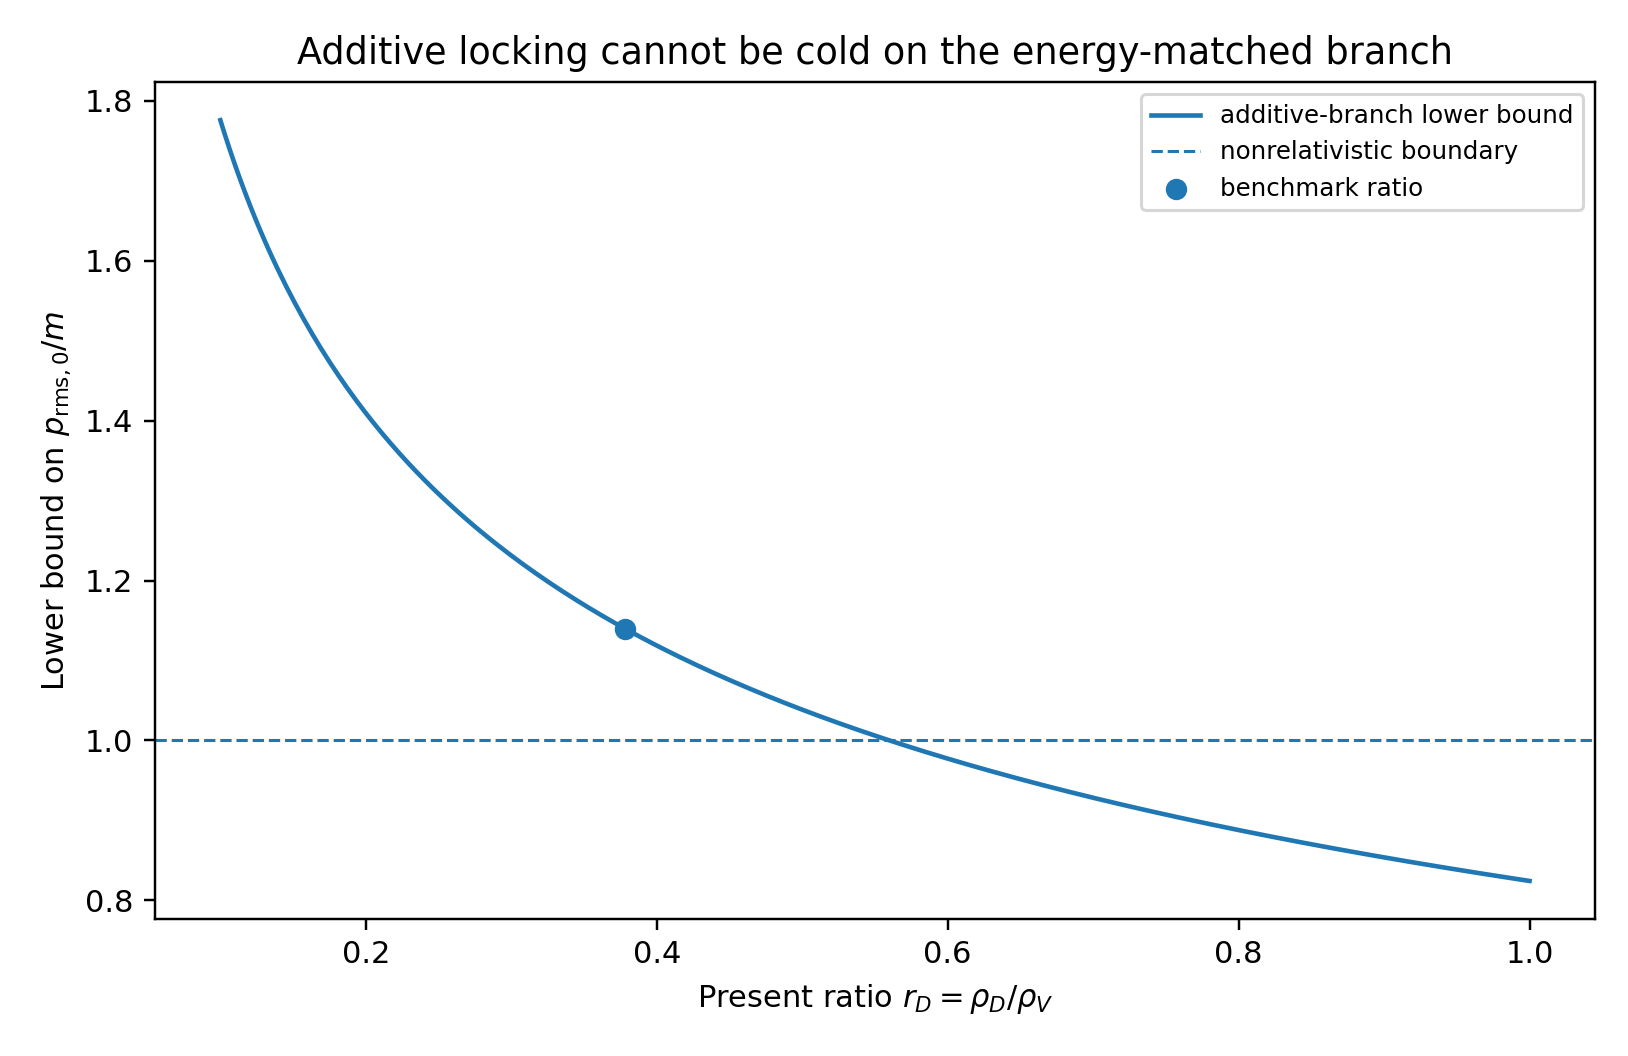
\includegraphics[width=0.90\linewidth]{figures/scw/additive_branch_obstruction.png}
\caption{The abundance, energy-matching, and locking conditions force the additive one-shell ratio $p_{\rm rms}/m$ above unity at the declared present density ratio, contradicting the assumed cold branch.}
\label{fig:scw-additive-obstruction}
\end{figure}

\section{Scale-covariant fiber action}

Let
\begin{equation}
 U(\phi)=\frac{\lambda}{4}(\phi^2-v^2)^2,
 \qquad
 \mu^2=\lambda v^2,
 \label{eq:scw-average-potential}
\end{equation}
and let
\begin{equation}
 \mathcal L_{\sigma,p}
 =\Lambda^2\sum_{h\geq1}p^{2\sigma h}\mathsf D_h.
 \label{eq:scw-fiber-operator}
\end{equation}
The scale-covariant branch is defined by
\begin{equation}
\boxed{
\begin{aligned}
 S_{\rm SC}
 =-\int\sqrt{-g}\,d^4x\Bigg[
 &\frac12(\partial\phi)^2+U(\phi)
 +\frac12\langle\partial\chi,\partial\chi\rangle_p\\
 &+\frac12\left\langle
 \chi,
 \left(
 m_0^2-\mu^2
 +\left(1+\gamma\frac{\phi^2}{v^2}\right)
 \mathcal L_{\sigma,p}
 \right)\chi
 \right\rangle_p
 \Bigg].
\end{aligned}}
 \label{eq:scw-action}
\end{equation}
The level masses at the locked origin are
\begin{equation}
 m_h^2
 =m_0^2-\mu^2+\Lambda^2p^{2\sigma h},
 \label{eq:scw-level-masses}
\end{equation}
with multiplicities
\begin{equation}
 d_h=(p-1)p^{h-1}.
 \label{eq:scw-level-degeneracy}
\end{equation}
The average mode now changes the internal refinement scale itself.  Its homogeneous equation is
\begin{equation}
 \ddot\phi+3H\dot\phi
 +\lambda\phi(\phi^2-v^2)
 +\frac{\gamma\phi}{v^2}Y_D=0,
 \label{eq:scw-average-eom}
\end{equation}
where
\begin{equation}
 Y_D
 :=\sum_h\Lambda^2p^{2\sigma h}X_h,
 \qquad
 X_h:=\langle\chi_h^2\rangle.
 \label{eq:scw-weighted-lock-source}
\end{equation}
The origin curvature is
\begin{equation}
 \boxed{
 M_\phi^2
 =-\mu^2+\frac{\gamma}{v^2}Y_D.}
 \label{eq:scw-lock-curvature}
\end{equation}
For nonrelativistic levels with $m_h^2\gg\mu^2,m_0^2$,
\begin{equation}
 \Lambda^2p^{2\sigma h}X_h
 =\rho_h\left[1+O(w_h)+O\left(\frac{\mu^2+m_0^2}{m_h^2}\right)\right].
 \label{eq:scw-weighted-energy-limit}
\end{equation}
Thus the total cold dark density, including heavy levels, supplies the locking source.

\section{Weighted nonadiabatic production}

Near a crossing,
\begin{equation}
 \phi(t)=\dot\phi_\star(t-t_\star)+O((t-t_\star)^2),
 \label{eq:scw-crossing-linearization}
\end{equation}
so that
\begin{equation}
 \omega_{h,k}^2
 =k^2+m_h^2
 +\frac{\gamma\Lambda^2p^{2\sigma h}}{v^2}
 \dot\phi_\star^2(t-t_\star)^2.
 \label{eq:scw-crossing-frequency}
\end{equation}
Define
\begin{equation}
 A_\star:=\frac{\sqrt\gamma|\dot\phi_\star|}{v},
 \qquad
 \nu_h:=A_\star\Lambda p^{\sigma h}.
 \label{eq:scw-weighted-rate}
\end{equation}
The rapid-crossing spectrum is
\begin{equation}
 \boxed{
 f_h(k)
 =\eta
 \exp\left[-\frac{\pi(k^2+m_h^2)}{\nu_h}\right],}
 \label{eq:scw-weighted-occupation}
\end{equation}
where $\eta$ is fixed by energy projection when the linearized spectrum would exceed the available kinetic energy:
\begin{equation}
 \eta
 =\min\left(1,\frac{K_\star}{\widetilde\rho_\star}\right).
 \label{eq:scw-energy-projection}
\end{equation}
This is not an independent abundance fit.  It is the shape-preserving rapid-crossing approximation with exact total-energy matching.

At high level,
\begin{equation}
 m_h\simeq\Lambda p^{\sigma h},
 \qquad
 \nu_h\simeq A_\star m_h.
 \label{eq:scw-high-level-law}
\end{equation}
The suppression exponent becomes linear rather than quadratic in mass:
\begin{equation}
 \frac{\pi m_h^2}{\nu_h}
 \simeq\frac{\pi m_h}{A_\star}.
 \label{eq:scw-linear-mass-suppression}
\end{equation}
At the same time,
\begin{equation}
 \frac{p_{\rm rms,\star}}{m_h}
 \simeq
 \sqrt{\frac{3A_\star}{2\pi m_h}},
 \label{eq:scw-heavy-colder}
\end{equation}
so heavier populated levels are born colder.

\section{Exact \texorpdfstring{$\sigma=1$}{sigma=1} continuum theorem}

For $\sigma=1$, the endpoint law
\begin{equation}
 N(m)=\frac{m}{\Lambda}-1
 \label{eq:scw-state-count}
\end{equation}
gives the continuum density of levels
\begin{equation}
 \frac{dN}{dm}=\frac1\Lambda.
 \label{eq:scw-density-of-levels}
\end{equation}
Using $\nu=Am$ and the occupation \eqref{eq:scw-weighted-occupation}, the number and captured rest-density spectra are
\begin{equation}
 \frac{dn}{dm}
 =\eta\frac{A^{3/2}}{8\pi^3\Lambda}
 m^{3/2}e^{-\pi m/A},
 \label{eq:scw-number-spectrum}
\end{equation}
\begin{equation}
 \boxed{
 \frac{d\rho_R}{dm}
 =\eta\frac{A^{3/2}}{8\pi^3\Lambda}
 m^{5/2}e^{-\pi m/A}.}
 \label{eq:scw-rest-spectrum}
\end{equation}
The selected mass band peaks at
\begin{equation}
 \boxed{
 m_{\rm peak}=\frac{5A}{2\pi}.}
 \label{eq:scw-mass-peak}
\end{equation}
The exact continuum integrals are
\begin{equation}
 n_\star=C_N\eta\frac{A^4}{\Lambda},
 \qquad
 C_N=\frac{3}{32\pi^5},
 \label{eq:scw-number-constant}
\end{equation}
\begin{equation}
 \rho_{R,\star}=C_R\eta\frac{A^5}{\Lambda},
 \qquad
 C_R=\frac{15}{64\pi^6},
 \label{eq:scw-rest-constant}
\end{equation}
\begin{equation}
 \rho_\star=C_E\eta\frac{A^5}{\Lambda},
 \qquad
 C_E=\frac{32}{35\pi^7},
 \label{eq:scw-energy-constant}
\end{equation}
\begin{equation}
 p_\star=C_P\eta\frac{A^5}{\Lambda},
 \qquad
 C_P=\frac{32}{315\pi^7}.
 \label{eq:scw-pressure-constant}
\end{equation}
For example, the total-energy coefficient follows from the Tricomi representation and the beta integral:
\begin{equation}
\begin{aligned}
 C_E
 &=\frac{1}{2\pi^2}
 \int_0^\infty y^2e^{-\pi y}I_\rho(\sqrt y)\,dy\\
 &=\frac{6}{\pi^7}B\left(\frac32,3\right)
 =\frac{32}{35\pi^7}.
\end{aligned}
 \label{eq:scw-energy-beta-proof}
\end{equation}
Consequently,
\begin{equation}
 \boxed{
 w_\star=\frac{p_\star}{\rho_\star}=\frac19,}
 \label{eq:scw-production-w}
\end{equation}
\begin{equation}
 \boxed{
 f_R:=\frac{\rho_{R,\star}}{\rho_\star}
 =\frac{525\pi}{2048}
 =0.8053399136\ldots,}
 \label{eq:scw-rest-fraction}
\end{equation}
and
\begin{equation}
 \frac{\rho_{R,\star}}{n_\star}
 =\frac{5A}{2\pi}
 =m_{\rm peak}.
 \label{eq:scw-mean-mass}
\end{equation}

A dyadic discrete tower with $\Lambda/A=10^{-4}$ gives
\begin{equation}
 f_R^{(2)}=0.8054331018,
 \qquad
 w_\star^{(2)}=0.1110616168,
 \label{eq:scw-discrete-ratios}
\end{equation}
and selects
\begin{equation}
 \frac{m_{\rm peak}^{(2)}}A=0.8192,
 \label{eq:scw-discrete-peak}
\end{equation}
within one dyadic bin of \eqref{eq:scw-mass-peak}.  The absolute normalization retains the known log-periodic prime modulation, while the ratios are nearly envelope independent.

\begin{figure}[htbp]
\centering
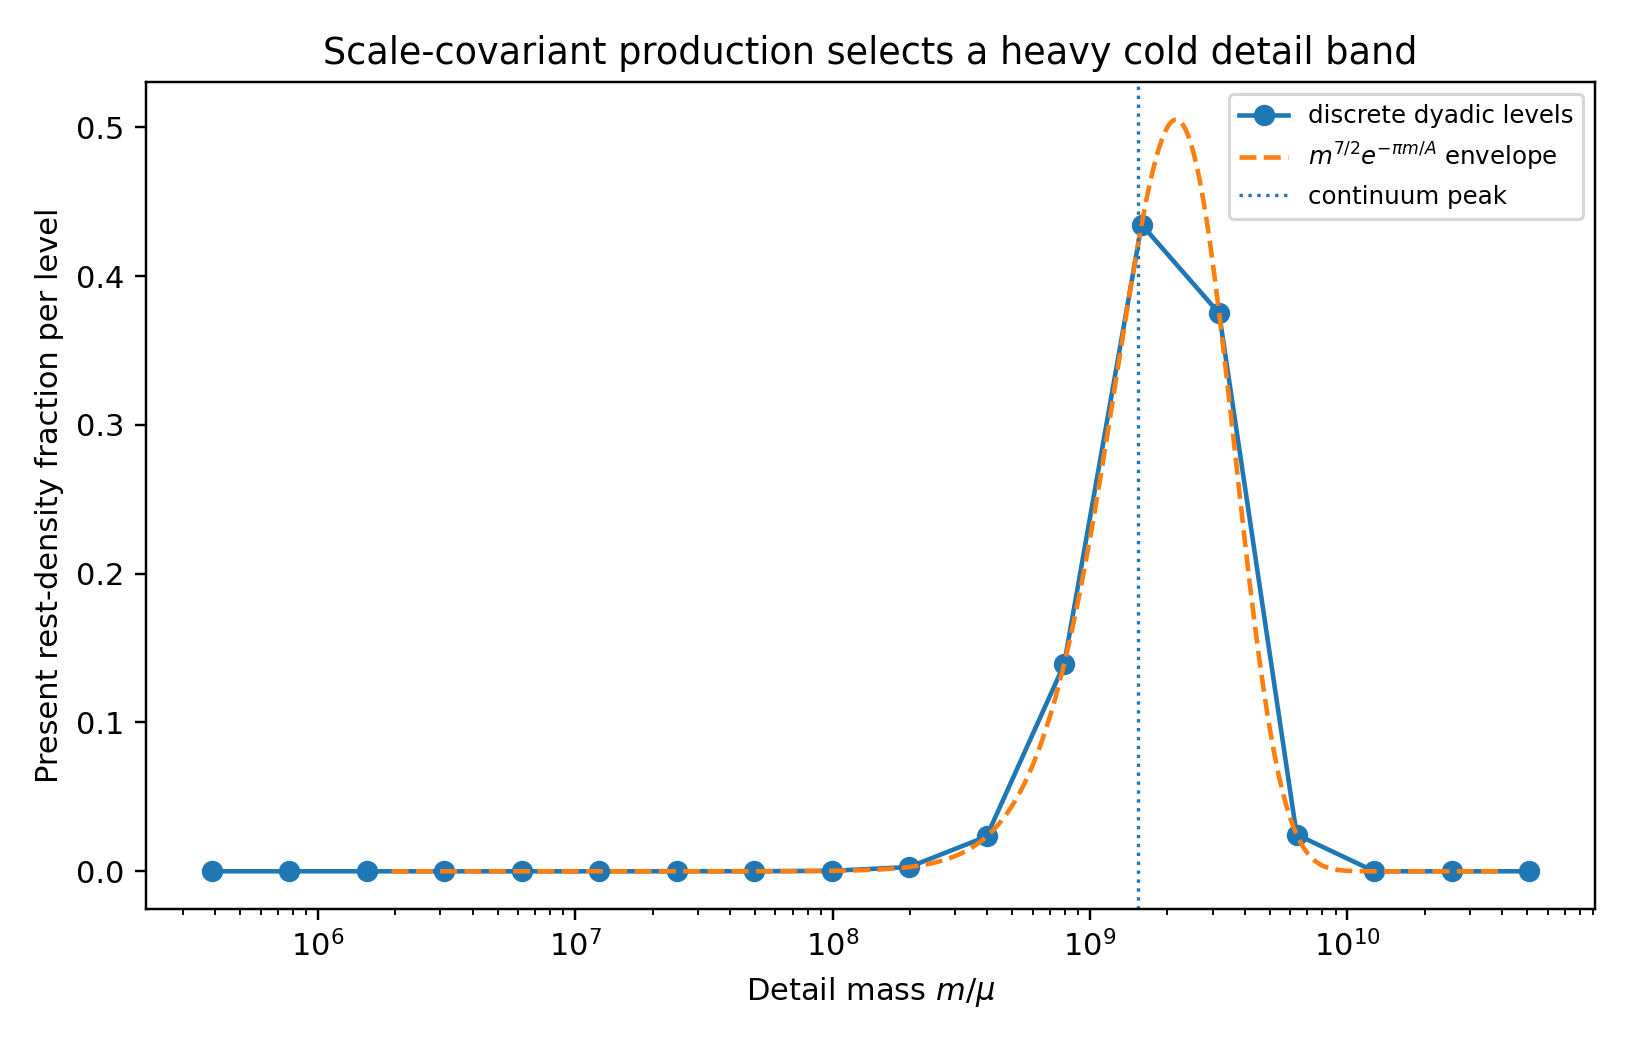
\includegraphics[width=0.92\linewidth]{figures/scw/weighted_detail_mass_spectrum.png}
\caption{The discrete dyadic rest-density fractions follow the analytic scale-covariant mass envelope.  The dominant mass is many orders of magnitude above the vacuum scale in the calibrated benchmark.}
\label{fig:scw-mass-spectrum}
\end{figure}

\section{Abundance calibration and emergent hierarchy}

On the captured branch,
\begin{equation}
 \rho_{R,\star}=f_RK_\star.
 \label{eq:scw-captured-rest}
\end{equation}
After the produced band becomes nonrelativistic,
\begin{equation}
 \rho_{D0}=f_RK_\star a_\star^3.
 \label{eq:scw-present-abundance}
\end{equation}
Define
\begin{equation}
 F:=\frac{K_\star}{\rho_V}.
 \label{eq:scw-F-definition}
\end{equation}
The present abundance fixes
\begin{equation}
 \boxed{
 F=\frac{r_D}{f_Ra_\star^3}.}
 \label{eq:scw-F-calibration}
\end{equation}
The crossing scale and selected mass are then
\begin{equation}
 \frac{A_\star}{\mu}
 =\sqrt{\frac{\gamma F}{2}},
 \label{eq:scw-A-over-mu}
\end{equation}
\begin{equation}
 \boxed{
 \frac{m_{\rm peak}}\mu
 =\frac{5}{2\pi}
 \sqrt{\frac{\gamma r_D}{2f_Ra_\star^3}}.}
 \label{eq:scw-peak-hierarchy}
\end{equation}
If the average field begins at rest at $\phi_i$, then
\begin{equation}
 F
 =\left(\frac{\phi_i}{v}\right)^4
 -2\left(\frac{\phi_i}{v}\right)^2,
 \label{eq:scw-initial-energy}
\end{equation}
so
\begin{equation}
 \boxed{
 \frac{|\phi_i|}{v}
 =\sqrt{1+\sqrt{1+F}}.}
 \label{eq:scw-initial-amplitude}
\end{equation}
Thus one early production scale determines both the hierarchy between the vacuum and dark-matter masses and the required pre-crossing field amplitude.

For the benchmark
\begin{equation}
 a_\star=10^{-6},
 \qquad
 \gamma=16,
 \qquad
 p=2,
 \qquad
 \frac{\Lambda}{A_\star}=10^{-4},
 \label{eq:scw-benchmark-inputs}
\end{equation}
with \eqref{eq:scw-rd-benchmark}, the discrete calculation gives
\begin{equation}
 \frac{K_\star}{\rho_V}
 =4.6969787254\times10^{17},
 \label{eq:scw-benchmark-F}
\end{equation}
\begin{equation}
 \frac{A_\star}{\mu}
 =1.9384486014\times10^9,
 \qquad
 \frac{|\phi_i|}{v}=2.6179096175\times10^4,
 \label{eq:scw-benchmark-hierarchy}
\end{equation}
\begin{equation}
 \boxed{
 \frac{m_{\rm peak}^{(2)}}\mu
 =1.5879770943\times10^9.}
 \label{eq:scw-benchmark-peak}
\end{equation}
The shape-preserving energy projection is
\begin{equation}
 \eta=3.8062069178\times10^{-21}.
 \label{eq:scw-benchmark-eta}
\end{equation}
This small occupation per microscopic state is compensated by the large refinement multiplicities.  It is determined by energy conservation after the rapid-crossing spectrum is assembled.

\section{Coldness theorem and cutoff scale}

At $a\gg a_\star$, the scale-covariant continuum band obeys
\begin{equation}
 \boxed{
 w_D(a)=\frac{a_\star^2}{5a^2},}
 \label{eq:scw-late-w}
\end{equation}
\begin{equation}
 \boxed{
 c_{a,D}^2(a)=\frac{a_\star^2}{3a^2},}
 \label{eq:scw-late-ca}
\end{equation}
and
\begin{equation}
 \boxed{
 v_{\rm rms}(a)
 =\sqrt{\frac35}\frac{a_\star}{a}.}
 \label{eq:scw-late-speed}
\end{equation}
Unlike the additive one-shell result, the present speed decreases directly with the production scale.  The reason is that the selected mass grows with the crossing rate while its fractional production momentum decreases as $m^{-1/2}$.

For $a_\star=10^{-6}$,
\begin{equation}
 w_{D0}=1.9987378335\times10^{-13},
 \qquad
 v_{\rm rms,0}=7.7459666924\times10^{-7}.
 \label{eq:scw-benchmark-coldness}
\end{equation}
The fluid Jeans estimate is
\begin{equation}
 \frac{k_J(a)}{aH(a)}
 =\sqrt{\frac{3\Omega_m(a)}{2c_{a,D}^2(a)}},
 \label{eq:scw-jeans-definition}
\end{equation}
which gives
\begin{equation}
 \boxed{
 \frac{k_J(a)}{H_0}
 =\frac{3}{\sqrt2}
 \frac{\sqrt{\Omega_{m0}a}}{a_\star}.}
 \label{eq:scw-jeans-law}
\end{equation}
At the present epoch,
\begin{equation}
 \frac{k_{J0}}{H_0}=1.1811011811\times10^6.
 \label{eq:scw-benchmark-jeans}
\end{equation}

\section{Density locking and transient acceleration}

Using \eqref{eq:scw-weighted-energy-limit}, the locked cold branch satisfies
\begin{equation}
 \frac{M_\phi^2}{\mu^2}
 =-1+\frac{\gamma}{4}r_D(a)
 +O(w_D)+O\left(\frac{\mu^2}{m_{\rm eff}^2}\right).
 \label{eq:scw-lock-density-law}
\end{equation}
Hence present locking requires
\begin{equation}
 \boxed{
 \gamma>\frac{4}{r_{D0}}.}
 \label{eq:scw-gamma-lock}
\end{equation}
For the declared ratio, the right side is $10.573\ldots$.  The benchmark choice $\gamma=16$ gives
\begin{equation}
 \boxed{
 \frac{M_\phi^2(1)}{\mu^2}=0.5132408576.}
 \label{eq:scw-present-lock-curvature}
\end{equation}
The exact discrete kinetic moments reconstruct
\begin{equation}
 \frac{Y_D(1)}{\rho_V}=0.3783102144
 \label{eq:scw-weighted-source-numeric}
\end{equation}
within $2.3\times10^{-13}$ of the declared dark-density ratio.

The cold asymptotic release scale is
\begin{equation}
 a_{\rm release}
 =\left(\frac{\gamma r_{D0}}4\right)^{1/3}.
 \label{eq:scw-release-law}
\end{equation}
The exact discrete result is
\begin{equation}
 \boxed{
 a_{\rm release}=1.1480726020.}
 \label{eq:scw-release-numeric}
\end{equation}
For baryon ratio
\begin{equation}
 r_{b0}=0.0710237567,
 \label{eq:scw-rb-benchmark}
\end{equation}
the acceleration onset is
\begin{equation}
 \boxed{
 a_{\rm acc}=0.6081134084,}
 \label{eq:scw-acceleration-numeric}
\end{equation}
with a cold asymptotic estimate differing by $1.94\times10^{-4}$.

At the locked point, the quadratic average-mode action remains
\begin{equation}
 S_{\delta\phi}^{(2)}
 =\frac12\int a^3dt\,d^3x
 \left[
 \delta\dot\phi^2
 -\frac{(\nabla\delta\phi)^2}{a^2}
 -M_\phi^2\delta\phi^2
 \right].
 \label{eq:scw-perturbation-action}
\end{equation}
Therefore
\begin{equation}
 Q_{\delta\phi}=1,
 \qquad
 c_{s,\phi}^2=1,
 \qquad
 M_\phi^2>0
 \label{eq:scw-perturbation-stability}
\end{equation}
throughout the locked interval.  Because every mass deformation is even in $\phi$, the detail stress tensor also has no term linear in $\delta\phi$ at $\phi=0$.

\begin{figure}[htbp]
\centering
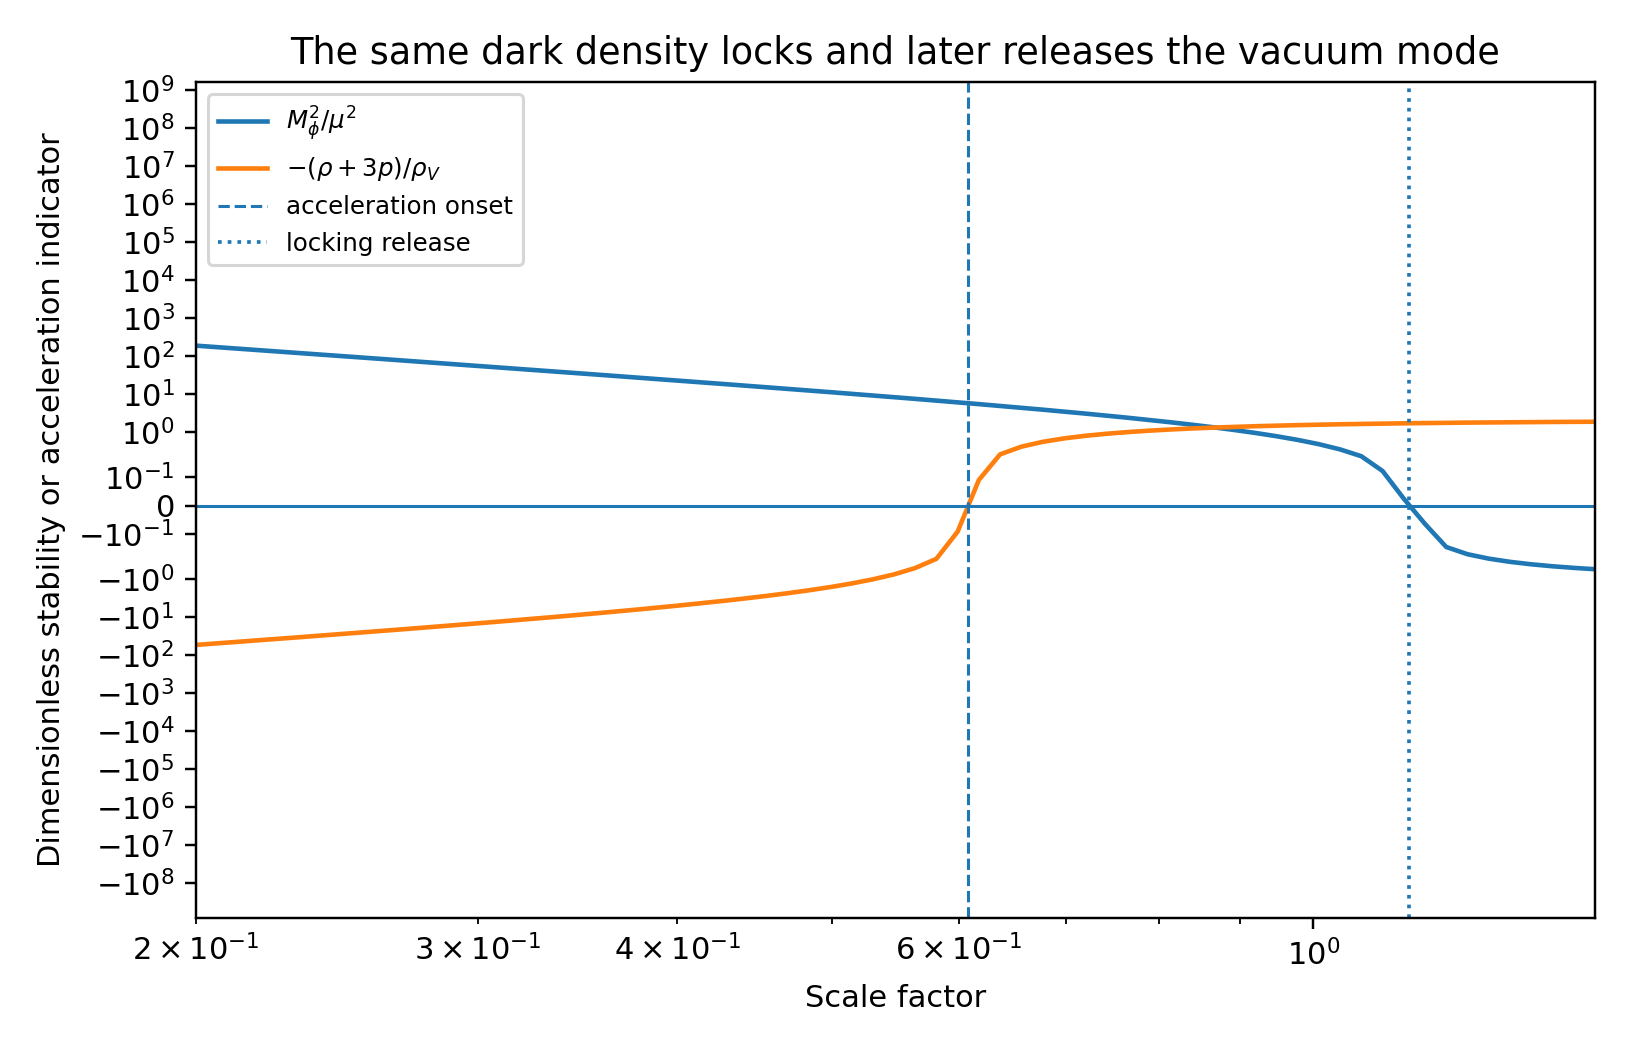
\includegraphics[width=0.92\linewidth]{figures/scw/weighted_locking_and_release.png}
\caption{The weighted detail density stabilizes the average mode well before acceleration begins.  Dilution eventually removes the locking curvature and releases the vacuum mode.}
\label{fig:scw-lock-release}
\end{figure}

\section{Linear growth and lensing benchmark}

For $a\gg a_\star$, use $N=\log a$ and the controlled cold-fluid closure
\begin{equation}
 \delta_b''
 +\left(2+\frac{d\log H}{dN}\right)\delta_b'
 =\frac32S,
 \label{eq:scw-baryon-growth}
\end{equation}
\begin{equation}
 \delta_D''
 +\left(2+\frac{d\log H}{dN}\right)\delta_D'
 +\frac{c_{a,D}^2k^2}{a^2H^2}\delta_D
 =\frac32S,
 \label{eq:scw-dark-growth}
\end{equation}
where
\begin{equation}
 S=\Omega_b(a)\delta_b+\Omega_D(a)\delta_D.
 \label{eq:scw-growth-source}
\end{equation}
The same source controls the subhorizon lensing potential to the accuracy of this closure.

Starting at $a_i=10^{-3}$ with adiabatic growing data, the benchmark gives
\begin{center}
\begin{tabular}{rcc}
\toprule
$k/H_0$ & $\delta_D/\delta_{D,{\rm cold}}$ & lensing source / cold source\\
\midrule
$30$ & $0.9999996989$ & $0.9999997007$\\
$300$ & $0.9999698901$ & $0.9999700727$\\
$3000$ & $0.9969926202$ & $0.9970108463$\\
$10000$ & $0.9669918115$ & $0.9671896257$\\
$30000$ & $0.7331608409$ & $0.7346038042$\\
$100000$ & $0.0159173474$ & $0.0169297429$\\
\bottomrule
\end{tabular}
\end{center}
The first half-mode of the fluid lensing-source transfer is
\begin{equation}
 \boxed{
 \frac{k_{1/2}}{H_0}=4.4076353413\times10^4.}
 \label{eq:scw-half-mode}
\end{equation}
For the conditional conversion $H_0=70\,\mathrm{km\,s^{-1}\,Mpc^{-1}}$,
\begin{equation}
 k_{1/2}=10.2916022620\,\mathrm{Mpc}^{-1}.
 \label{eq:scw-half-mode-mpc}
\end{equation}
This is a fluid-closure benchmark, not yet a complete collisionless Einstein--Boltzmann likelihood.

\begin{figure}[htbp]
\centering
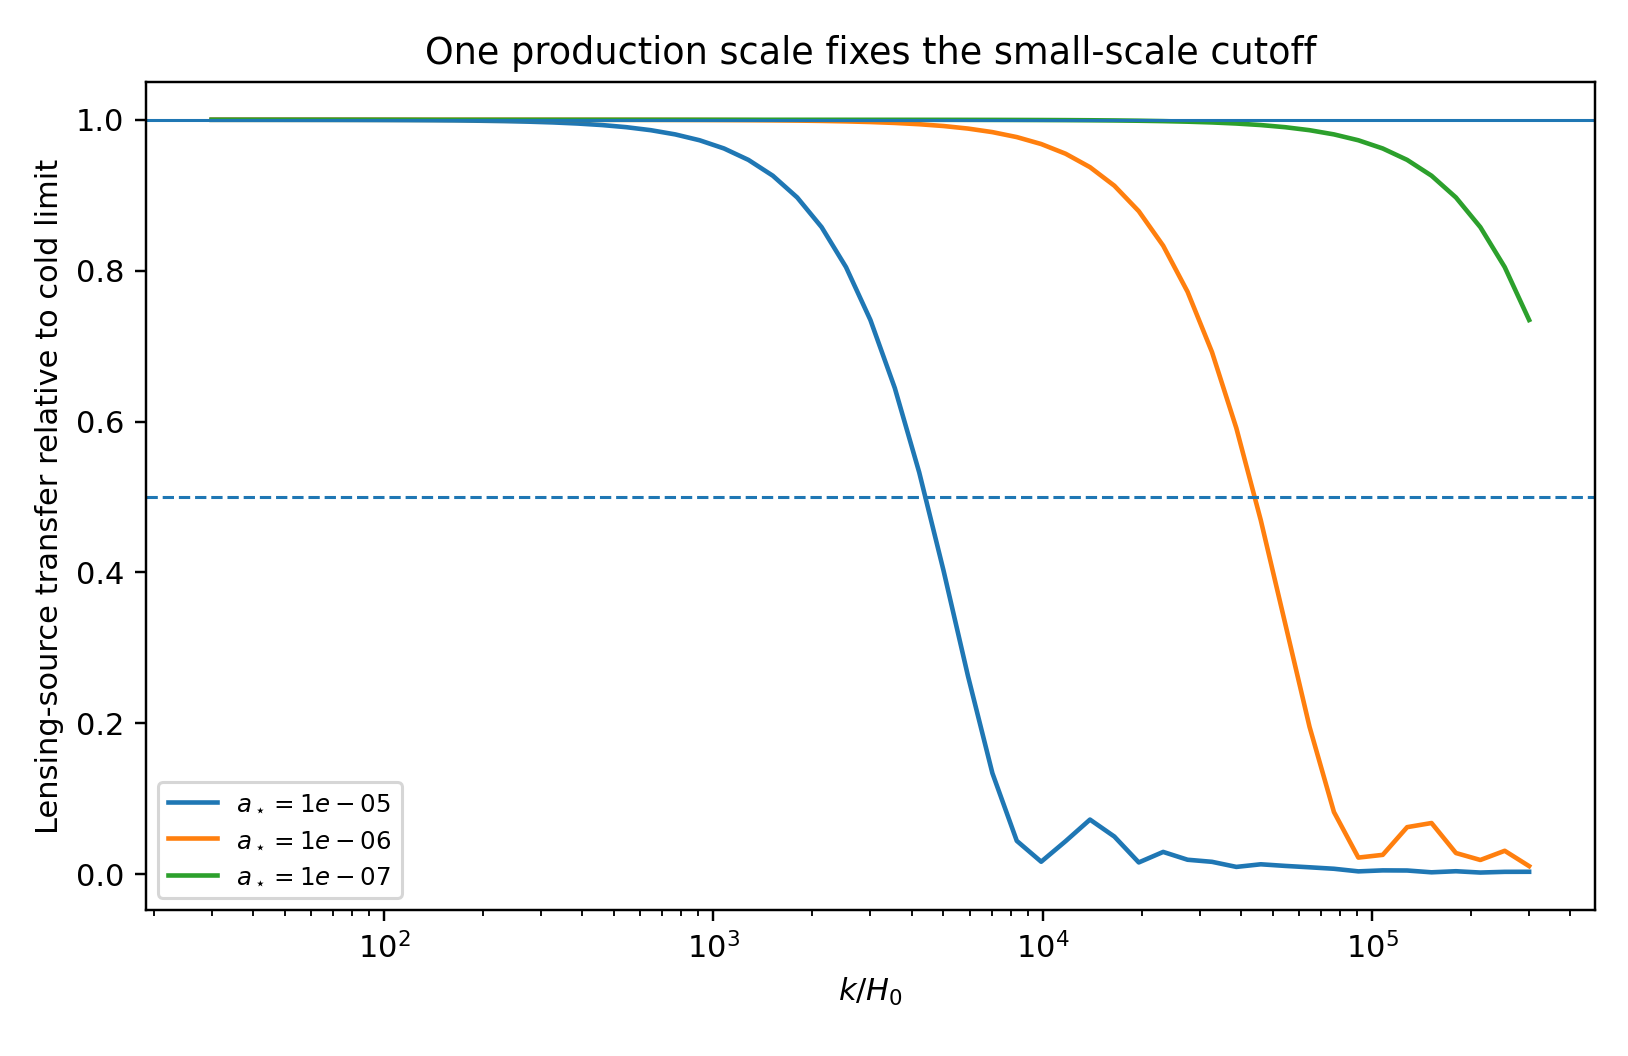
\includegraphics[width=0.92\linewidth]{figures/scw/weighted_transfer_suppression.png}
\caption{The production epoch controls the free-streaming cutoff without changing the late locking law.  The high-$k$ oscillations are those of the finite sound-speed fluid closure.}
\label{fig:scw-transfer}
\end{figure}

\section{Verification ledger}

The deterministic calculation records twenty passes and no failures.  Selected checks are
\begin{center}
\begin{tabular}{p{0.64\linewidth}r}
\toprule
statement & residual\\
\midrule
additive abundance--velocity elimination identity & $0$\\
continuum $C_E$ versus independent quadrature & $1.62\times10^{-12}$ relative\\
continuum $C_P$ versus independent quadrature & $3.49\times10^{-11}$ relative\\
discrete versus continuum captured rest fraction & $9.32\times10^{-5}$\\
discrete versus continuum production $w$ & $4.95\times10^{-5}$\\
present abundance reconstruction & $0$\\
exact versus asymptotic release scale & $1.95\times10^{-13}$\\
exact versus asymptotic acceleration scale & $1.93\times10^{-4}$\\
exact kinetic $c_a^2$ versus $a_\star^2/(3a^2)$ & $6.31\times10^{-4}$ relative\\
large-scale lensing-source deviation at $k/H_0=300$ & $2.99\times10^{-5}$\\
\bottomrule
\end{tabular}
\end{center}
The executable records are
\begin{equation}
 R_{\rm SC}=\texttt{data/Scale\_Covariant\_Dark\_Sector\_Verification.json},
 \label{eq:scw-json-record}
\end{equation}
\begin{equation}
 C_{\rm SC}=\texttt{data/scale\_covariant\_dark\_checks.csv},
 \label{eq:scw-check-record}
\end{equation}
\begin{equation}
 X_{\rm SC}=\texttt{verification/Scale\_Covariant\_Dark\_Sector\_Verification.py}.
 \label{eq:scw-script-record}
\end{equation}

\section{Closure ledger and remaining burden}

\begin{center}
\begin{tabular}{@{}>{\raggedright\arraybackslash}p{0.47\linewidth}>{\raggedright\arraybackslash}p{0.18\linewidth}>{\raggedright\arraybackslash}p{0.27\linewidth}@{}}
\toprule
statement & status & boundary\\
\midrule
additive one-shell cold-lock obstruction & proved conditional & rapid, energy-matched, dominant-shell branch\\
scale-covariant fiber action & defined & one new coupling $\gamma$\\
weighted production spectrum & derived & linear rapid crossing\\
$\sigma=1$ continuum mass theorem & proved & high-level density-of-states envelope\\
energy-projected rest fraction & proved & shape-preserving capture approximation\\
late $w_D$, $c_a^2$, and $v_{\rm rms}$ laws & proved asymptotically & collisionless nonrelativistic regime\\
density locking and release & closed controlled & heavy-level limit and regular locked phase\\
linear growth and lensing cutoff & numerical controlled & two-fluid sound-speed closure\\
full collisionless hierarchy & open & momentum and anisotropic-stress multipoles\\
radiative stability of scale covariance & open & quantum effective action\\
microscopic derivation of $\gamma$ and $a_\star$ & open & gravitational refinement dynamics\\
observational likelihood and priority audit & open & independent implementation and data comparison\\
\bottomrule
\end{tabular}
\end{center}

The principal result is not that every earlier dark-sector formula survives unchanged.  The hard consistency audit rejects the additive dominant-shell mechanism and identifies a minimal viable replacement:
\begin{equation}
 \boxed{
 \begin{gathered}
 \text{average-mode dilation of the refinement spectrum}\\
 \Longrightarrow \text{ heavy cold detail band}\\
 \Longrightarrow \text{ density-weighted vacuum locking}
 \end{gathered}}
 \label{eq:scw-result-chain}
\end{equation}
A complete physical treatment therefore requires the full collisionless Einstein--Boltzmann hierarchy for the distribution \eqref{eq:scw-weighted-occupation}, with one parameter set propagated through recombination, matter power, weak lensing, and the transient-release background without sector-by-sector renormalization.

\chapter{Scale-Covariant Collisionless Boltzmann Dynamics and Late-Time Observables}
\PhysicsContext{From a distribution to observables}{The third part carries one prescribed distribution through momentum-resolved transport, photon and neutrino hierarchies, recombination, reionization, line-of-sight projection, and CMB lensing. These are controlled templates, not a precision replacement for production codes.}


\label{ch:collisionless-boltzmann-observables}

\section{Scope and objective}

The scale-covariant refinement dark sector fixes a discrete mass spectrum, a production distribution, a cold late-time limit, and a density-dependent locking source.  The preceding growth calculation replaced that distribution by one adiabatic sound speed.  That fluid closure is adequate on large scales but does not retain momentum dependence, free streaming, or the higher angular moments of the collisionless distribution.

This chapter develops the kinetic layer in two stages.  First, it derives the complete linear collisionless hierarchy for every retained refinement level and momentum node.  Second, it specializes that hierarchy to a controlled post-recombination, subhorizon Einstein--Vlasov--Poisson system and propagates one fixed scale-covariant distribution into matter-power, redshift-space-growth, weak-lensing, and CMB-lensing templates.

The numerical section begins at
\begin{equation}
 a_i=10^{-3}.
 \label{eq:cb-initial-scale}
\end{equation}
Adiabatic perturbations are prescribed at that surface.  The calculation therefore measures the \emph{incremental post-recombination transfer} generated between $a_i$ and today; it does not evolve free streaming from the production event to $a_i$.  Radiation is retained in the background expansion but its perturbations are not included in the late-time Poisson source.  Consequently the section does not compute primary CMB temperature or polarization spectra, recombination kinetics, neutrino transport, or superhorizon metric evolution.  The CMB result below is a late-time lensing template and a scale-separation diagnostic, not a primary-anisotropy likelihood.

\section{Scale-covariant phase-space distribution}

For each retained detail level $h$, let
\begin{equation}
 m_h=\Lambda p^{\sigma h},
 \qquad
 d_h=(p-1)p^{h-1},
 \label{eq:cb-level-data}
\end{equation}
within the high-level scale-covariant branch.  The rapid-crossing distribution has the form
\begin{equation}
 \bar f_h(q)
 =\eta\exp\left[-\frac{\pi m_h^2}{\nu_h}
 -\frac{\pi q^2}{a_\star^2\nu_h}\right],
 \qquad
 \nu_h=A_\star m_h.
 \label{eq:cb-background-distribution}
\end{equation}
For the benchmark used here, $A_\star$ is the mass unit, $p=2$, $\sigma=1$, and
\begin{equation}
 \frac{\Lambda}{A_\star}=10^{-4},
 \qquad
 a_\star=10^{-6}.
 \label{eq:cb-benchmark-production}
\end{equation}
The common energy-projection normalization $\eta$ cancels from every linear transfer ratio.

The conformal energy is
\begin{equation}
 \epsilon_h(q,a)=\sqrt{q^2+a^2m_h^2},
 \label{eq:cb-conformal-energy}
\end{equation}
and the background density and pressure are
\begin{equation}
 \rho_h(a)
 =\frac{d_h}{2\pi^2a^4}
 \int_0^\infty q^2\epsilon_h\bar f_h\,dq,
 \label{eq:cb-background-density}
\end{equation}
\begin{equation}
 p_h(a)
 =\frac{d_h}{6\pi^2a^4}
 \int_0^\infty \frac{q^4}{\epsilon_h}\bar f_h\,dq.
 \label{eq:cb-background-pressure}
\end{equation}
The numerical phase grid retains the ten levels carrying all but less than $10^{-6}$ of the present rest-density weight.  Their retained weights sum to unity to $2.3\times10^{-16}$.

\section{Complete linear collisionless hierarchy}

Use conformal Newtonian gauge,
\begin{equation}
 ds^2=a^2(\eta)
 \left[-(1+2\Psi)d\eta^2+(1-2\Phi)d\mathbf x^2\right].
 \label{eq:cb-newtonian-gauge}
\end{equation}
Write the perturbed distribution as
\begin{equation}
 f_h(\mathbf k,q,\mu,\eta)
 =\bar f_h(q)
 \left[1+\mathcal F_h(\mathbf k,q,\mu,\eta)\right],
 \label{eq:cb-distribution-perturbation}
\end{equation}
where $\mu=\widehat{\mathbf k}\cdot\widehat{\mathbf q}$, and expand
\begin{equation}
 \mathcal F_h
 =\sum_{\ell\geq0}
 (-i)^\ell(2\ell+1)
 F_{h\ell}(k,q,\eta)P_\ell(\mu).
 \label{eq:cb-multipole-expansion}
\end{equation}
Set
\begin{equation}
 D_h(q):=\frac{d\log\bar f_h}{d\log q}.
 \label{eq:cb-log-derivative}
\end{equation}
The linear collisionless Boltzmann equation gives
\begin{equation}
 \dot F_{h0}
 =-k\frac{q}{\epsilon_h}F_{h1}
 +\dot\Phi D_h,
 \label{eq:cb-hierarchy-zero}
\end{equation}
\begin{equation}
 \dot F_{h1}
 =\frac{kq}{3\epsilon_h}
 \left(F_{h0}-2F_{h2}\right)
 -\frac{k\epsilon_h}{3q}\Psi D_h,
 \label{eq:cb-hierarchy-one}
\end{equation}
\begin{equation}
 \dot F_{h\ell}
 =\frac{kq}{(2\ell+1)\epsilon_h}
 \left[\ell F_{h,\ell-1}-(\ell+1)F_{h,\ell+1}\right],
 \qquad \ell\geq2.
 \label{eq:cb-hierarchy-general}
\end{equation}
These equations retain the complete angular hierarchy of the produced distribution.  No sound speed is inserted.

The stress-energy moments are
\begin{equation}
 \delta\rho_h
 =\frac{d_h}{2\pi^2a^4}
 \int q^2\epsilon_h\bar f_hF_{h0}\,dq,
 \label{eq:cb-delta-rho}
\end{equation}
\begin{equation}
 \delta p_h
 =\frac{d_h}{6\pi^2a^4}
 \int \frac{q^4}{\epsilon_h}\bar f_hF_{h0}\,dq,
 \label{eq:cb-delta-p}
\end{equation}
\begin{equation}
 (\rho_h+p_h)\theta_h
 =\frac{d_hk}{2\pi^2a^4}
 \int q^3\bar f_hF_{h1}\,dq,
 \label{eq:cb-theta}
\end{equation}
\begin{equation}
 (\rho_h+p_h)\sigma_h
 =\frac{d_h}{3\pi^2a^4}
 \int \frac{q^4}{\epsilon_h}\bar f_hF_{h2}\,dq.
 \label{eq:cb-sigma}
\end{equation}
Thus density, pressure, velocity, and anisotropic stress are all projections of one hierarchy.

\section{Post-recombination Vlasov--Poisson specialization}

For the controlled late-time calculation, the time derivative of the spatial metric potential is neglected relative to the subhorizon force term.  The hierarchy becomes a Vlasov system sourced by
\begin{equation}
 k^2\Psi
 =-4\pi Ga^2
 \left(\rho_b\delta_b+\sum_h\delta\rho_h\right).
 \label{eq:cb-poisson}
\end{equation}
The baryon equations are
\begin{equation}
 \dot\delta_b=-\theta_b,
 \qquad
 \dot\theta_b+\mathcal H\theta_b=k^2\Psi.
 \label{eq:cb-baryon-fluid}
\end{equation}
Let $N=\log a$, $E(a)=H(a)/H_0$, and
\begin{equation}
 \kappa(a):=\frac{k}{aH}=\frac{k/H_0}{aE(a)}.
 \label{eq:cb-kappa}
\end{equation}
Then the implemented hierarchy is
\begin{equation}
 \frac{dF_{h0}}{dN}
 =-\kappa\frac{q}{\epsilon_h}F_{h1},
 \label{eq:cb-n-hierarchy-zero}
\end{equation}
\begin{equation}
 \frac{dF_{h1}}{dN}
 =\kappa
 \left[
 \frac{q}{3\epsilon_h}(F_{h0}-2F_{h2})
 -\frac{\epsilon_h}{3q}\Psi D_h
 \right],
 \label{eq:cb-n-hierarchy-one}
\end{equation}
with the corresponding $N$-form of \eqref{eq:cb-hierarchy-general}.

The background is not replaced by exact dust.  It uses the same phase-space quadrature as the hierarchy:
\begin{equation}
 E(a)^2
 =\Omega_{r0}a^{-4}
 +\Omega_{b0}a^{-3}
 +\Omega_{D0}\frac{\rho_D(a)}{\rho_D(1)}
 +\Omega_{V0}.
 \label{eq:cb-background-hubble}
\end{equation}
The locked average mode has no linear stress perturbation in this phase and enters only through $\Omega_{V0}$.

\section{Adiabatic growing initialization}

At $a_i=10^{-3}$, the retained tower is already highly nonrelativistic.  Set
\begin{equation}
 F_{h0}(q,N_i)=\delta_i,
 \qquad
 \delta_i=a_i.
 \label{eq:cb-initial-monopole}
\end{equation}
Let
\begin{equation}
 u_i:=\frac{\theta_i}{\mathcal H_i}=-\delta_i,
 \qquad
 \kappa_i:=\frac{k}{\mathcal H_i}.
 \label{eq:cb-initial-velocity}
\end{equation}
The momentum-dependent boost initialization is
\begin{equation}
 F_{h1}(q,N_i)
 =\frac{u_i}{\kappa_i}
 \left[-\frac{D_h(q)}{3v_h(q,N_i)}\right],
 \qquad
 v_h:=\frac{q}{\epsilon_h}.
 \label{eq:cb-initial-dipole}
\end{equation}
For the Gaussian production distribution,
\begin{equation}
 D_h=-2\pi x^2,
 \qquad
 x=\frac{q}{a_\star\sqrt{\nu_h}},
 \label{eq:cb-gaussian-derivative}
\end{equation}
and
\begin{equation}
 \frac{
 \int_0^\infty x^2e^{-\pi x^2}(-D_h/3)\,dx
 }{
 \int_0^\infty x^2e^{-\pi x^2}\,dx
 }
 =1.
 \label{eq:cb-boost-identity}
\end{equation}
Hence the hierarchy reproduces the growing-mode continuity normalization in the cold limit without assigning one artificial velocity to every momentum node.

\section{Multipole and momentum closure}

Momentum integration uses generalized Gauss--Laguerre quadrature with weight $y^{1/2}e^{-y}$.  The declared production transfer is converged to
\begin{equation}
 \epsilon_q=3.05\times10^{-5}
 \label{eq:cb-quadrature-residual}
\end{equation}
when increasing the quadrature from eight to ten nodes per retained level.

For the angular tail, define the free-streaming distance
\begin{equation}
 s_h(q,N)
 :=\int_{N_i}^{N}
 \frac{q/\epsilon_h}{aE(a)}\,dN.
 \label{eq:cb-stream-distance}
\end{equation}
When $ks_h>L+1$, use the spherical-Bessel recurrence closure
\begin{equation}
 F_{h,L+1}
 =\frac{2L+1}{ks_h}F_{hL}-F_{h,L-1}.
 \label{eq:cb-recurrence-closure}
\end{equation}
The free hierarchy reproduces $F_\ell=j_\ell(x)$ through the tested low multipoles with maximum residual
\begin{equation}
 \epsilon_{\rm fs}=9.52\times10^{-9}.
 \label{eq:cb-free-streaming-residual}
\end{equation}
The $L=6$ to $L=8$ present-transfer difference on the declared convergence sample is
\begin{equation}
 \epsilon_L=3.62\times10^{-5}.
 \label{eq:cb-ell-residual}
\end{equation}

\section{Matter and Weyl transfer functions}

Define the total matter contrast and the Poisson/Weyl source by
\begin{equation}
 \delta_m
 =\frac{\rho_b\delta_b+\rho_D\delta_D}{\rho_b+\rho_D},
 \label{eq:cb-total-matter}
\end{equation}
\begin{equation}
 \begin{aligned}
 S_W={}&\Omega_{b0}a^{-1}\delta_b
 +\Omega_{D0}a^2\frac{\rho_D(a)}{\rho_D(1)}\delta_D\\
 &-\frac32\Omega_{D0}a^2\frac{\rho_D(a)}{\rho_D(1)}
 (1+w_D)\sigma_D.
 \end{aligned}
 \label{eq:cb-weyl-source}
\end{equation}
The last term is the collisionless gravitational-slip contribution.  It is retained in the lensing source even though it is numerically tiny for the declared cold benchmark.
Relative to a pressureless reference evolved from the same initial amplitude, set
\begin{equation}
 T_m(k,a)=\frac{\delta_m(k,a)}{\delta_m^{\rm cold}(a)},
 \qquad
 T_W(k,a)=\frac{S_W(k,a)}{S_W^{\rm cold}(a)}.
 \label{eq:cb-transfer-definitions}
\end{equation}
The linear matter-power ratio is
\begin{equation}
 \frac{P_m(k,a)}{P_m^{\rm cold}(k,a)}=T_m(k,a)^2.
 \label{eq:cb-power-ratio}
\end{equation}

The post-recombination transfer is unity on large scales and develops a finite incremental free-streaming cutoff.  The amplitude half-mode is
\begin{equation}
 \boxed{
 \frac{k_{1/2}^{(T)}}{H_0}=4.71448\times10^4,}
 \label{eq:cb-amplitude-half-mode}
\end{equation}
while the power half-mode is
\begin{equation}
 \boxed{
 \frac{k_{1/2}^{(P)}}{H_0}=3.14535\times10^4.}
 \label{eq:cb-power-half-mode}
\end{equation}
For the conditional conversion $H_0=70\,\mathrm{km\,s^{-1}\,Mpc^{-1}}$,
\begin{equation}
 \boxed{
 k_{1/2}^{(T)}=11.0081\,\mathrm{Mpc}^{-1},
 \qquad
 k_{1/2}^{(P)}=7.34423\,\mathrm{Mpc}^{-1}.}
 \label{eq:cb-half-mode-physical}
\end{equation}
These conversions are benchmark conventions rather than a likelihood fit.

\begin{figure}[htbp]
\centering
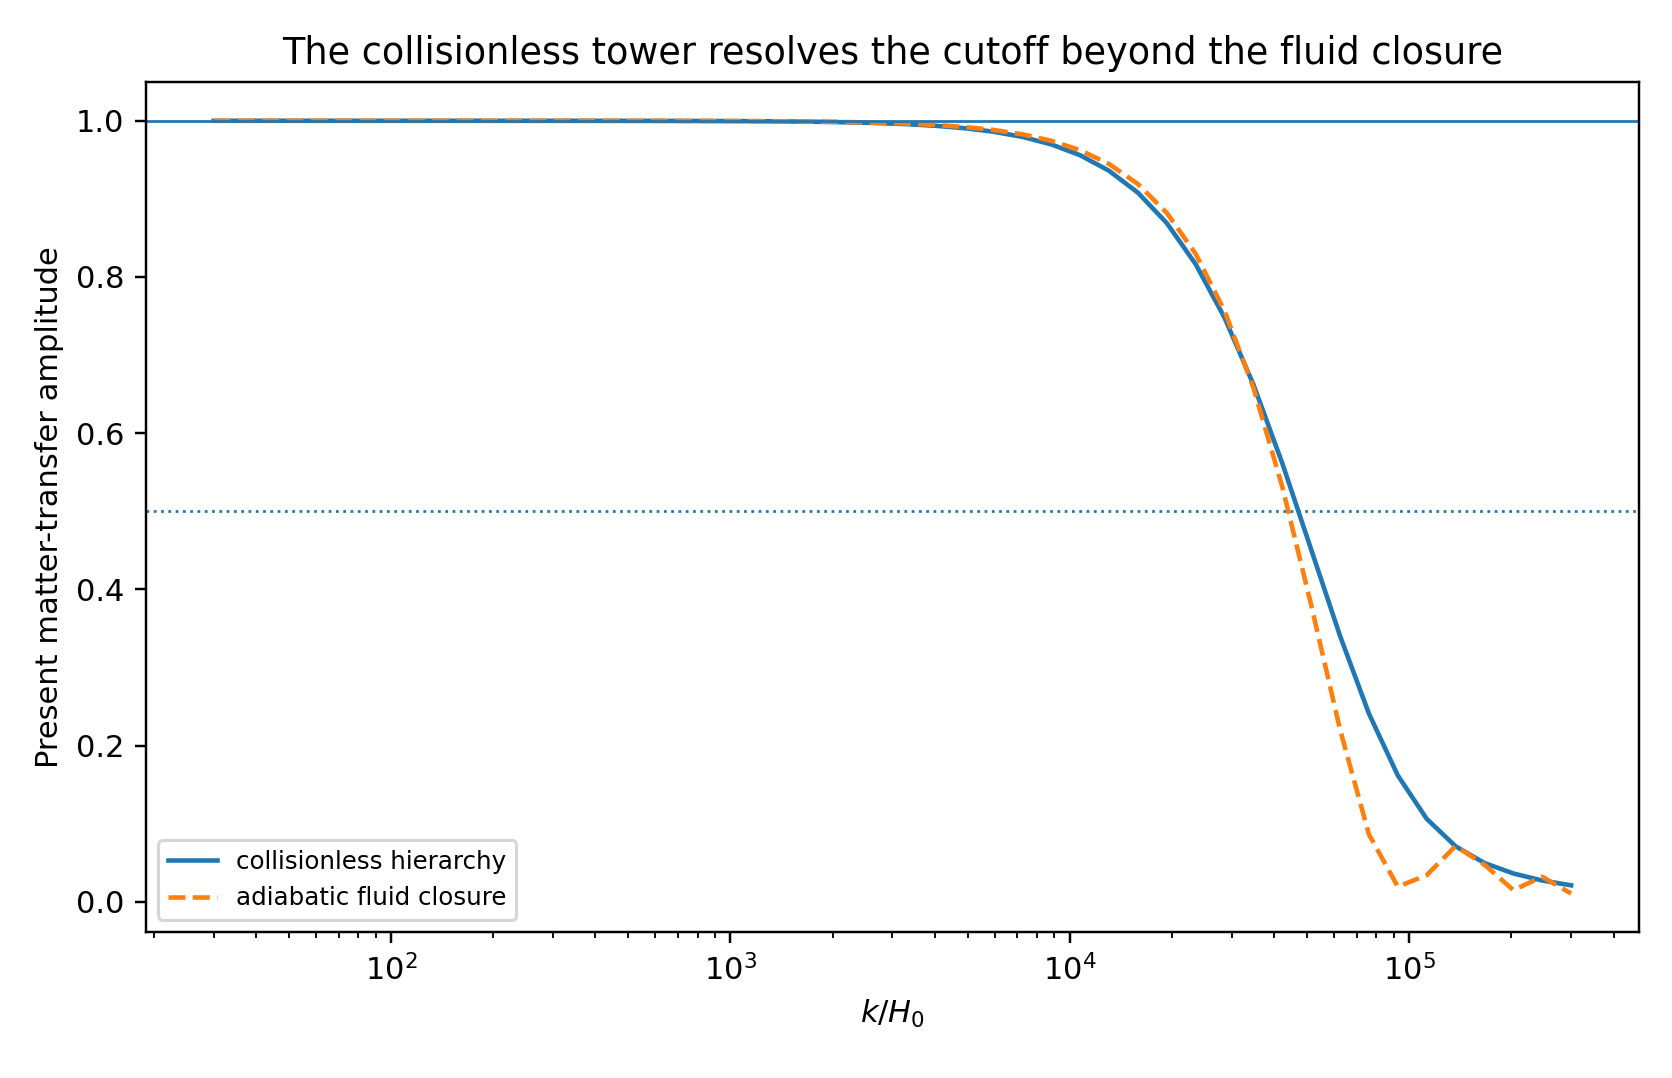
\includegraphics[width=0.88\linewidth]{figures/cb/collisionless_vs_fluid_transfer.png}
\caption{The collisionless hierarchy and the earlier adiabatic-fluid closure agree at large scale but differ materially after free streaming populates higher angular moments.}
\label{fig:cb-collisionless-fluid}
\end{figure}

Selected present values are
\begin{center}
\begin{tabular}{rrrr}
\toprule
$k/H_0$ & $T_m$ & $P_m/P_m^{\rm cold}$ & $T_m^{\rm fluid}$\\
\midrule
$3.15\times10^2$ & 0.999960 & 0.999921 & 0.999967\\
$2.72\times10^3$ & 0.997044 & 0.994096 & 0.997542\\
$2.86\times10^4$ & 0.747869 & 0.559307 & 0.756672\\
$5.14\times10^4$ & 0.451041 & 0.203438 & 0.380038\\
$9.26\times10^4$ & 0.161800 & 0.026179 & 0.019458\\
$3.00\times10^5$ & 0.021197 & 0.000449 & 0.010676\\
\bottomrule
\end{tabular}
\end{center}
The hierarchy is not equivalent to replacing the distribution by a single sound speed.  The difference changes sign across the cutoff because the collisionless response contains phase mixing rather than one coherent acoustic oscillation.

\section{Redshift-space growth and anisotropic stress}

On the common logarithmic scale-factor grid, define
\begin{equation}
 f_m(k,a)=\frac{d\log\delta_m(k,a)}{d\log a}.
 \label{eq:cb-growth-rate}
\end{equation}
For equal primordial normalization, the scale-dependent redshift-space amplitude ratio is
\begin{equation}
 \mathcal R_{f\sigma_8}(k,a)
 =\frac{f_m\delta_m}{f_m^{\rm cold}\delta_m^{\rm cold}}.
 \label{eq:cb-fsigma-ratio}
\end{equation}
At $z=0$, the benchmark gives
\begin{equation}
 \mathcal R_{f\sigma_8}=0.9970
 \quad\text{at}\quad k/H_0\simeq2.72\times10^3,
 \label{eq:cb-fsigma-large}
\end{equation}
\begin{equation}
 \mathcal R_{f\sigma_8}=0.7471
 \quad\text{at}\quad k/H_0\simeq2.86\times10^4,
 \label{eq:cb-fsigma-mid}
\end{equation}
\begin{equation}
 \mathcal R_{f\sigma_8}=0.1603
 \quad\text{at}\quad k/H_0\simeq9.26\times10^4.
 \label{eq:cb-fsigma-small}
\end{equation}
The computed late-time anisotropic stress remains finite and is below $1.5\times10^{-12}$ on the selected observable table.  It is dynamically retained even though it is numerically small for this very cold benchmark.

\begin{figure}[htbp]
\centering
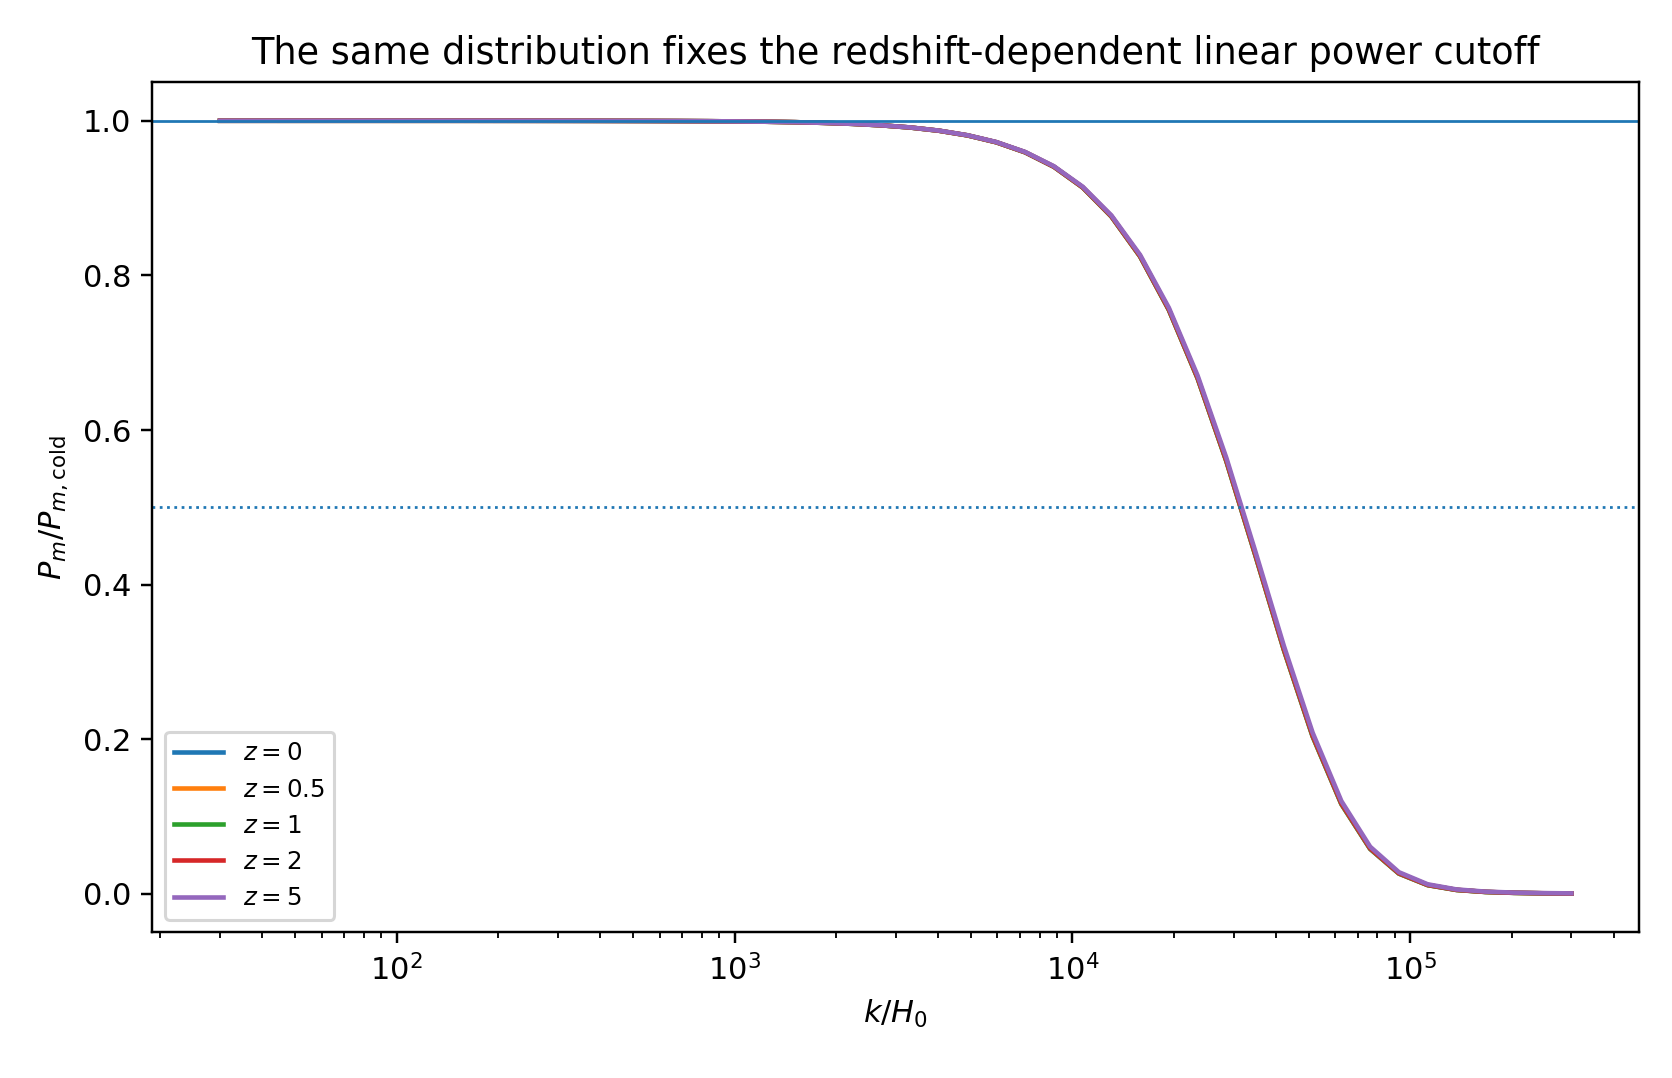
\includegraphics[width=0.88\linewidth]{figures/cb/matter_power_ratio_history.png}
\caption{The power cutoff develops continuously after the declared initial epoch.  The large scales remain locked to the cold reference while the high-$k$ modes lose coherent growth.}
\label{fig:cb-power-history}
\end{figure}

\section{Weak-lensing and CMB-lensing templates}

For a flat source plane at comoving distance $\chi_s$, define the controlled linear lensing ratio
\begin{equation}
 \mathcal R_\ell^\kappa
 =\frac{
 \int_0^{\chi_s}d\chi\,
 W(\chi,\chi_s)^2\chi^{-2}
 P_{\rm cold}(k,z)T_W(k,z)^2
 }{
 \int_0^{\chi_s}d\chi\,
 W(\chi,\chi_s)^2\chi^{-2}
 P_{\rm cold}(k,z)
 },
 \label{eq:cb-lensing-ratio}
\end{equation}
where
\begin{equation}
 k=\frac{\ell+1/2}{\chi}.
 \label{eq:cb-limber-map}
\end{equation}
The reference weight uses the same cold growth and the declared positive equality filter
\begin{equation}
 T_{\rm eq}(k)=\frac{1}{1+(k/k_{\rm eq})^2},
 \qquad
 \frac{k_{\rm eq}}{H_0}=\Omega_{m0}\sqrt{\frac{2}{\Omega_{r0}}}.
 \label{eq:cb-equality-filter}
\end{equation}
This is a normalized linear diagnostic.  It is not a nonlinear shear likelihood and does not include survey masks, intrinsic alignments, nonlinear baryonic feedback, or post-Born corrections.

For a galaxy source at $z_s=0.5$,
\begin{equation}
 \mathcal R_{1000}^{\kappa}=0.981331,
 \qquad
 \mathcal R_{3000}^{\kappa}=0.863481,
 \qquad
 \mathcal R_{5000}^{\kappa}=0.702128.
 \label{eq:cb-lensing-z05}
\end{equation}
For $z_s=1$,
\begin{equation}
 \mathcal R_{1000}^{\kappa}=0.993772,
 \qquad
 \mathcal R_{3000}^{\kappa}=0.949092,
 \qquad
 \mathcal R_{5000}^{\kappa}=0.874908.
 \label{eq:cb-lensing-z1}
\end{equation}
For a CMB source plane at the declared initial redshift $z_s=999$,
\begin{equation}
 \mathcal R_{1000}^{\kappa}=0.999615,
 \qquad
 \mathcal R_{2000}^{\kappa}=0.998474,
 \qquad
 \mathcal R_{3000}^{\kappa}=0.996591.
 \label{eq:cb-cmb-lensing}
\end{equation}

\begin{figure}[htbp]
\centering
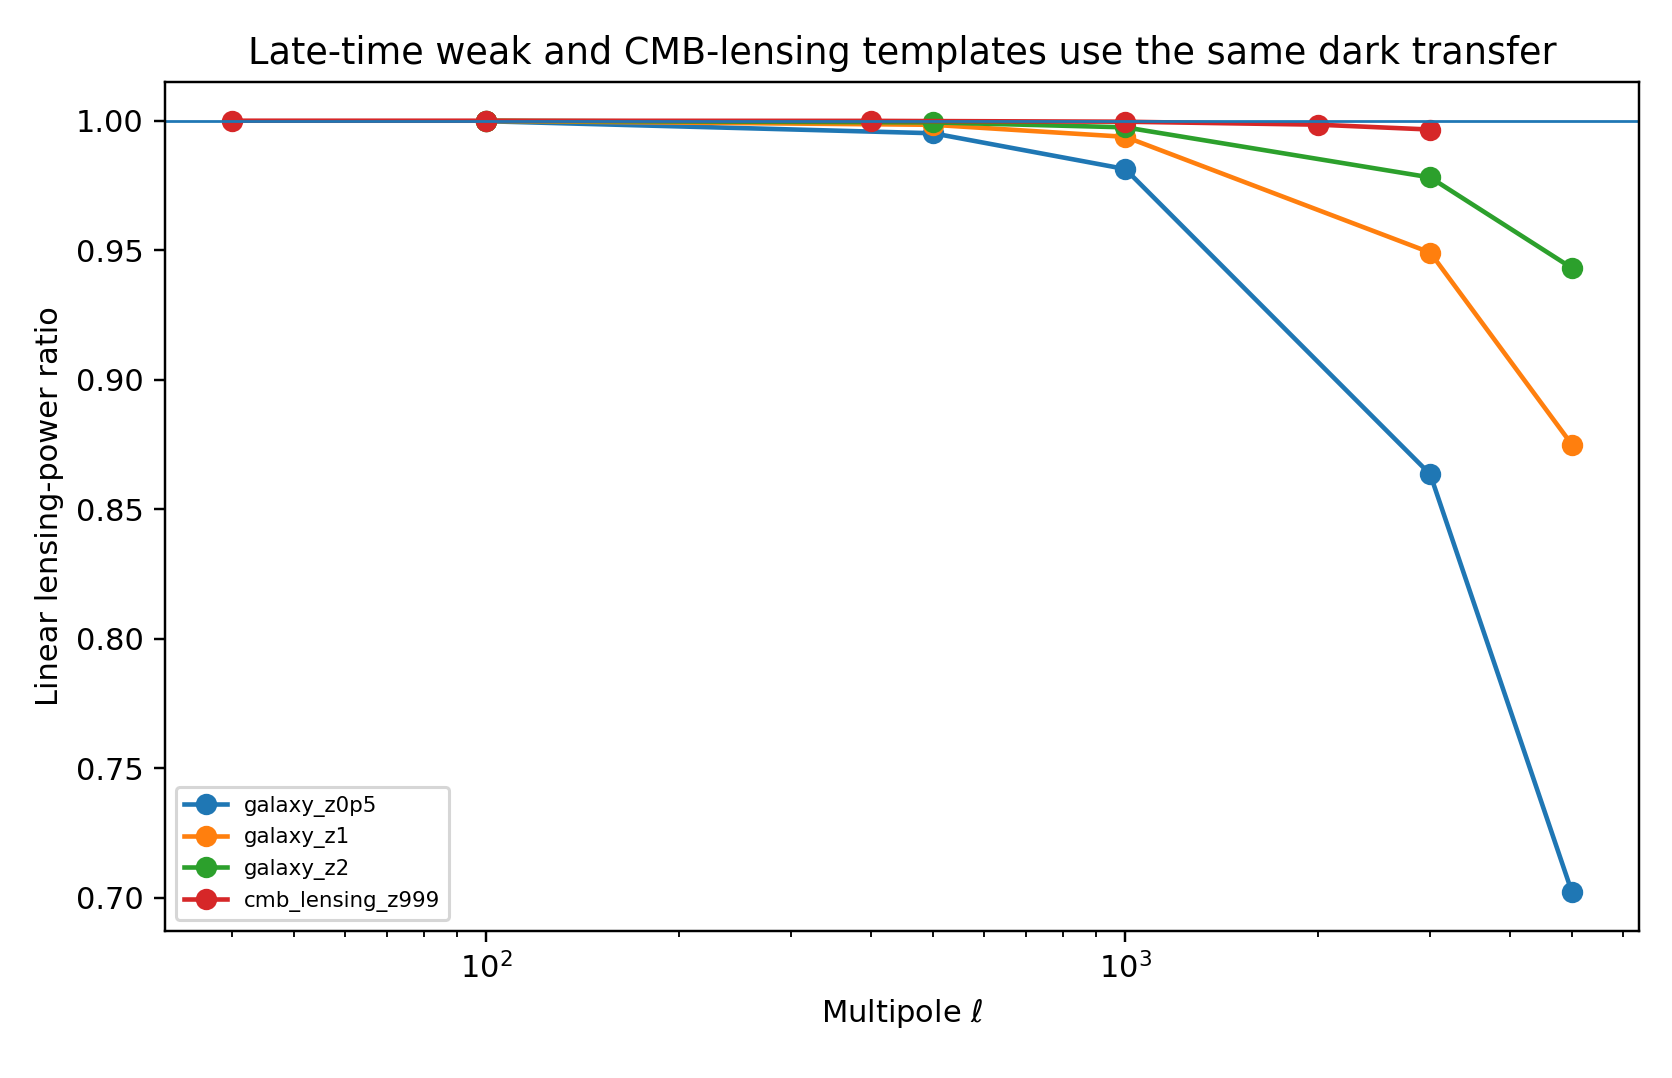
\includegraphics[width=0.88\linewidth]{figures/cb/lensing_power_ratios.png}
\caption{The late-time linear lensing response follows from the same collisionless Weyl transfer function without changing the dark parameters between clustering and lensing.}
\label{fig:cb-lensing-ratios}
\end{figure}

\section{Primary-CMB scale separation}

The comoving distance of the controlled background to $a=10^{-3}$ maps $\ell=3000$ to
\begin{equation}
 \left.\frac{k}{H_0}\right|_{\ell=3000}
 =957.699.
 \label{eq:cb-primary-k}
\end{equation}
This is only
\begin{equation}
 \boxed{
 \frac{k_{\ell=3000}}{k_{1/2}^{(P)}}=0.0304481}
 \label{eq:cb-primary-half-ratio}
\end{equation}
of the late-time power half-mode.  Thus the declared cutoff is parametrically separated from the primary acoustic scale.  This does not replace a primary TT, TE, or EE calculation.  It shows only a scale separation inside the declared late-time model.  Pre-$a_i$ free streaming, photon and neutrino metric driving, and recombination physics must be evolved before any statement about primary anisotropies is justified.

\section{Verification ledger}

The deterministic implementation records
\begin{equation}
 \boxed{20\ \mathrm{PASS},\qquad0\ \mathrm{FAIL}.}
 \label{eq:cb-check-count}
\end{equation}
The principal numerical controls are
\begin{center}
\begin{tabular}{lrr}
\toprule
control & coarse difference & fine difference\\
\midrule
momentum quadrature & $1.41\times10^{-4}$ & $3.05\times10^{-5}$\\
multipole truncation & $3.62\times10^{-5}$ & $3.62\times10^{-5}$\\
time-step refinement & $5.41\times10^{-8}$ & $1.89\times10^{-8}$\\
cold-production limit & -- & $4.01\times10^{-4}$\\
\bottomrule
\end{tabular}
\end{center}
The time-step sequence has an effective fitted order $1.52$ at the reported precision because the remaining error is already dominated by the moving angular closure and phase-space truncation.  The fine transfer difference itself is below $2\times10^{-8}$.

\section{Closure ledger}

\begin{center}
\begin{tabular}{>{\raggedright\arraybackslash}p{0.48\linewidth}>{\raggedright\arraybackslash}p{0.21\linewidth}>{\raggedright\arraybackslash}p{0.23\linewidth}}
\toprule
statement & status & boundary\\
\midrule
massive collisionless hierarchy for every retained level and momentum node & derived and implemented & linear perturbations\\
phase-space stress tensor including anisotropic stress & closed & declared quadrature\\
self-consistent baryon--tower Poisson source & closed controlled & quasi-static post-recombination regime\\
large-scale cold limit & numerically closed & declared hierarchy grid\\
post-recombination incremental transfer cutoff & numerically closed & prescribed data at $a_i$\\
scale-dependent $f\sigma_8$ template & closed controlled & linear theory\\
galaxy weak-lensing ratio & closed controlled & linear Limber template\\
CMB-lensing ratio & closed controlled & linear late-time lensing only\\
primary TT, TE, EE spectra & open & photon collisions and polarization\\
massless-neutrino hierarchy and recombination coupling & open & full Einstein--Boltzmann system\\
nonlinear matter power and halo formation & open & nonlinear solver or calibrated emulator\\
observational likelihood and parameter inference & open & external data and nuisance model\\
\bottomrule
\end{tabular}
\end{center}

\section{Synthesis and unresolved requirements}

The scale-covariant refinement distribution now determines, without replacing it by one sound speed,
\begin{equation}
 \boxed{
 \bar f_h(q)
 \Longrightarrow
 \{F_{h\ell}(q,k,a)\}
 \Longrightarrow
 \{T_m,T_W,f\sigma_8,\mathcal R_\ell^\kappa\}.}
 \label{eq:cb-result-chain}
\end{equation}
The same mass spectrum and production scale control dark clustering, redshift-space growth, galaxy lensing, and CMB lensing.

The unresolved kinetic and observational requirements are:
\begin{equation}
 \boxed{
 \begin{gathered}
 \text{add photons, polarization, baryons, and massless neutrinos},\\
 \text{couple the hierarchy through recombination and reionization},\\
 \text{compute TT, TE, EE, lensing, and }P_m(k)\text{ together},\\
 \text{then perform one joint likelihood without retuning the dark sector}.
 \end{gathered}}
 \label{eq:cb-open-requirements}
\end{equation}
\chapter{Controlled Production-to-Primary-CMB Einstein--Boltzmann Dynamics}
\label{ch:production-primary-cmb}

\section{Scope and objective}

The scale-covariant refinement dark sector now supplies a mass spectrum, a production distribution, a cold late-time limit, a collisionless perturbation hierarchy, and controlled late-time matter and lensing observables.  The remaining major linear-cosmology gap was the interval between production and last scattering.  In particular, the preceding late-time calculation did not jointly evolve photon collisions, polarization, baryons, massless neutrinos, metric driving, recombination, and the massive refinement hierarchy.

This chapter constructs that coupled system.  It evolves one unchanged dark-sector parameter set from
\begin{equation}
 a_{\star}=10^{-6}
 \label{eq:pcmb-production-scale}
\end{equation}
through recombination and beyond the visibility peak.  The numerical state contains photon temperature and polarization multipoles, baryon density and velocity, massless-neutrino multipoles, and momentum-resolved massive refinement multipoles.  The metric potentials are obtained from the Einstein momentum and anisotropic-stress equations, while the energy equation is retained as an independent diagnostic.

The resulting TT, TE, and EE spectra are \emph{controlled recombination-era templates}.  They demonstrate acoustic oscillations, polarization generation, neutrino and dark-sector metric feedback, finite-thickness damping, and a consistent geometric acoustic ruler.  They are not precision CMB likelihood spectra.  The calculation uses Saha hydrogen recombination, no reionization, no multilevel helium or hydrogen kinetics, no late integrated Sachs--Wolfe source, no lensing remapping, and a finite-width narrow-source projection rather than a production-quality line-of-sight integrator.

\section{One unchanged background and refinement distribution}

Use units in which wavenumbers and conformal rates are measured in $H_0$.  The background is
\begin{equation}
 E(a)^2
 =\Omega_{\gamma0}a^{-4}
 +\Omega_{\nu0}a^{-4}
 +\Omega_{b0}a^{-3}
 +\Omega_{D0}\frac{\rho_D(a)}{\rho_D(1)}
 +\Omega_{V0},
 \label{eq:pcmb-background}
\end{equation}
with
\begin{equation}
 \frac{\mathcal H}{H_0}=aE(a).
 \label{eq:pcmb-conformal-hubble}
\end{equation}
The declared numerical fractions are
\begin{equation}
 \Omega_{b0}=0.049,
 \qquad
 \Omega_{D0}=0.261,
 \qquad
 \Omega_{r0}=9.0\times10^{-5},
 \label{eq:pcmb-density-inputs}
\end{equation}
with $T_{\gamma0}=2.7255\,\mathrm K$ and $H_0=70\,\mathrm{km\,s^{-1}\,Mpc^{-1}}$ for the conditional conversion to physical units.  The blackbody photon density is computed from $T_{\gamma0}$,
\begin{equation}
 \Omega_{\gamma0}=5.0468884259\times10^{-5},
 \label{eq:pcmb-photon-density}
\end{equation}
and the remaining declared radiation density is assigned to a massless collisionless-neutrino sector,
\begin{equation}
 \Omega_{\nu0}=3.9531115741\times10^{-5}.
 \label{eq:pcmb-neutrino-density}
\end{equation}

For the scale-covariant refinement tower,
\begin{equation}
 m_h=A_{\star}\frac{\Lambda}{A_{\star}}p^{\sigma h},
 \qquad
 d_h=(p-1)p^{h-1},
 \label{eq:pcmb-level-spectrum}
\end{equation}
with
\begin{equation}
 p=2,
 \qquad
 \sigma=1,
 \qquad
 \frac{\Lambda}{A_{\star}}=10^{-4}.
 \label{eq:pcmb-dark-parameters}
\end{equation}
The produced distribution is proportional to
\begin{equation}
 \bar f_h(q)
 \propto
 \exp\left[-\pi\frac{m_h}{A_{\star}}
 -\pi\frac{q^2}{a_{\star}^2A_{\star}m_h}\right].
 \label{eq:pcmb-dark-distribution}
\end{equation}
Its common normalization is fixed by $\Omega_{D0}$ and cancels from the normalized perturbation transfer.  The background moments are
\begin{equation}
 \epsilon_h(q,a)=\sqrt{q^2+a^2m_h^2},
 \label{eq:pcmb-dark-energy}
\end{equation}
\begin{equation}
 \rho_D(a)
 =\frac{1}{2\pi^2a^4}
 \sum_h d_h\int_0^\infty q^2\epsilon_h\bar f_h\,dq,
 \label{eq:pcmb-dark-density}
\end{equation}
\begin{equation}
 p_D(a)
 =\frac{1}{6\pi^2a^4}
 \sum_h d_h\int_0^\infty\frac{q^4}{\epsilon_h}\bar f_h\,dq.
 \label{eq:pcmb-dark-pressure}
\end{equation}
Seven levels, $h=9,\ldots,15$, carry the retained present rest-density weight at the declared $10^{-4}$ threshold.  Two generalized Gauss--Laguerre nodes per level give fourteen massive phase-space nodes in the main solve.

At the visibility peak, the tower equation of state is
\begin{equation}
 \boxed{
 w_D(a_{\rm vis})
 =3.3085372607\times10^{-7}.}
 \label{eq:pcmb-dark-cold}
\end{equation}
The produced refinement sector is therefore already effectively cold during last scattering, while its momentum dependence and anisotropic stress remain explicitly present in the hierarchy.

\section{Saha recombination, opacity, and visibility}

Let
\begin{equation}
 T_\gamma(a)=\frac{T_{\gamma0}}{a},
 \qquad
 n_H(a)=\frac{(1-Y_p)\Omega_{b0}\rho_{c0}}{m_pa^3},
 \label{eq:pcmb-temperature-hydrogen}
\end{equation}
with $Y_p=0.24$.  The Saha ionization fraction obeys
\begin{equation}
 \frac{x_e^2}{1-x_e}
 =\frac{1}{n_H}
 \left(\frac{m_ek_BT_\gamma}{2\pi\hbar^2}\right)^{3/2}
 \exp\left(-\frac{\chi_H}{k_BT_\gamma}\right).
 \label{eq:pcmb-saha}
\end{equation}
Define the positive Thomson interaction rate
\begin{equation}
 \dot\kappa=a n_e\sigma_Tc,
 \label{eq:pcmb-opacity}
\end{equation}
where the dot denotes $d/d\eta$.  For $N=\log a$, the optical depth to the present is
\begin{equation}
 \tau(N)=\int_N^0\frac{\dot\kappa}{\mathcal H}\,dN,
 \label{eq:pcmb-optical-depth}
\end{equation}
and the visibility in logarithmic scale-factor measure is
\begin{equation}
 g_N(N)=e^{-\tau}\frac{\dot\kappa}{\mathcal H}.
 \label{eq:pcmb-visibility}
\end{equation}
The numerical integral gives
\begin{equation}
 \int g_N\,dN
 =0.9999798979,
 \label{eq:pcmb-visibility-integral}
\end{equation}
with peak
\begin{equation}
 \boxed{
 z_{\rm vis}=1286.261163,
 \qquad
 a_{\rm vis}=7.7684313701\times10^{-4}.}
 \label{eq:pcmb-visibility-peak}
\end{equation}

\begin{figure}[htbp]
\centering
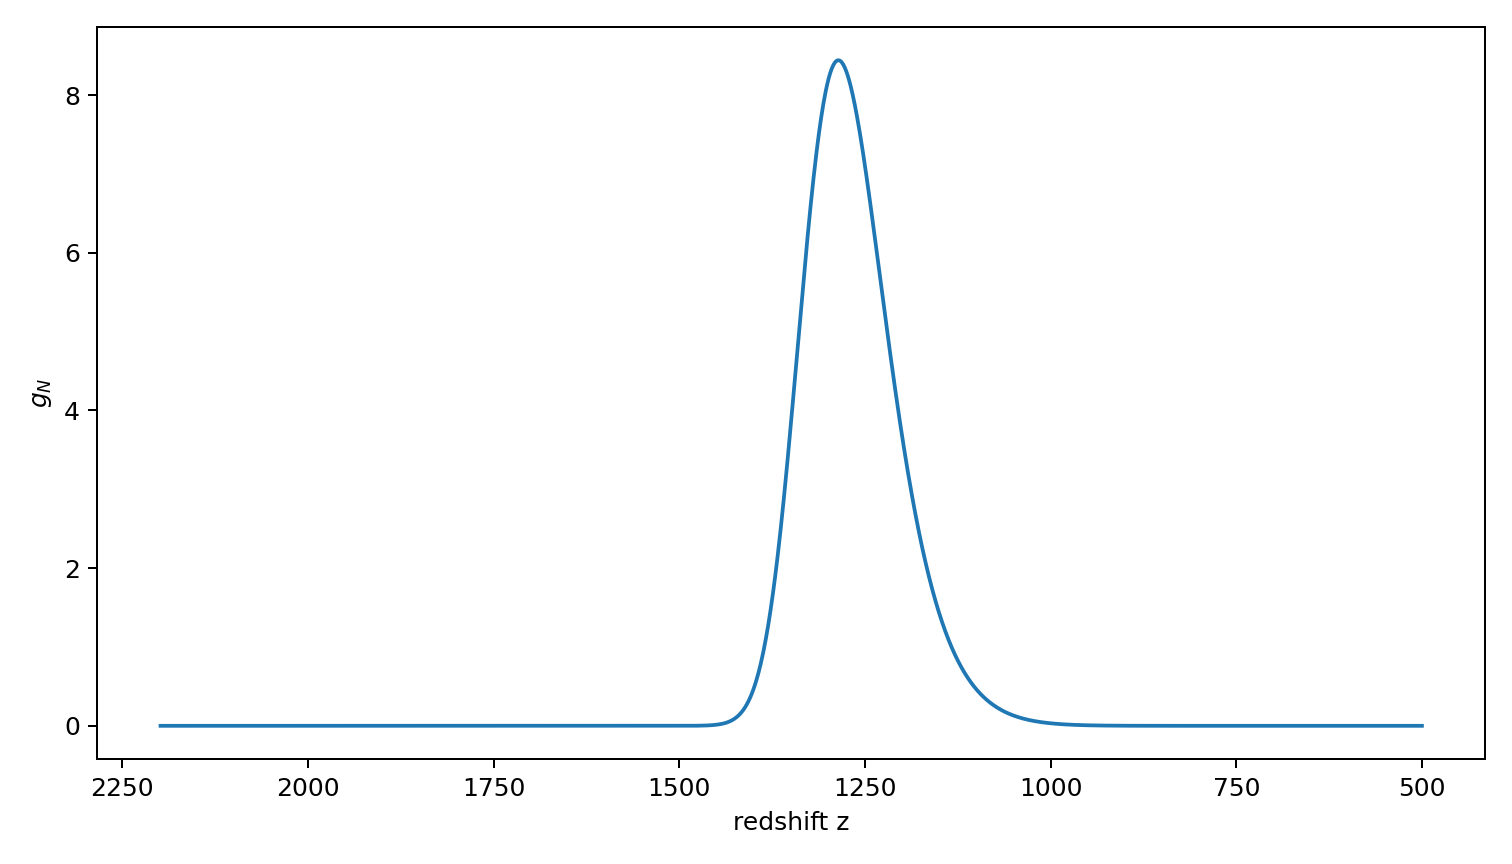
\includegraphics[width=0.88\linewidth]{figures/cmb/primary_cmb_visibility.png}
\caption{The controlled Saha visibility function in $d\log a$ measure.  The construction omits multilevel recombination, helium corrections beyond the fixed hydrogen fraction, and reionization.}
\label{fig:pcmb-visibility}
\end{figure}

\section{Metric conventions and Einstein closure}

Use conformal Newtonian gauge,
\begin{equation}
 ds^2=a^2(\eta)
 \left[-(1+2\Psi)d\eta^2+(1-2\Phi)d\mathbf x^2\right].
 \label{eq:pcmb-newtonian-gauge}
\end{equation}
Let
\begin{equation}
 \mathcal Q=\sum_s(\rho_s+p_s)\theta_s,
 \qquad
 \mathcal A=\sum_s(\rho_s+p_s)\sigma_s,
 \label{eq:pcmb-total-momentum-anis}
\end{equation}
where all densities are expressed in present critical-density units and $k$ is measured in $H_0$.  The implemented momentum and shear equations are
\begin{equation}
 \Phi'+\mathcal H\Psi
 =\frac{3}{2}\frac{a^2}{k^2}\mathcal Q,
 \label{eq:pcmb-einstein-momentum}
\end{equation}
\begin{equation}
 \Phi-\Psi
 =\frac{9}{2}\frac{a^2}{k^2}\mathcal A.
 \label{eq:pcmb-einstein-shear}
\end{equation}
The energy equation is not imposed after every step.  It is retained as an independent residual,
\begin{equation}
 \mathcal C_E
 :=k^2\Phi
 +3\mathcal H(\Phi'+\mathcal H\Psi)
 +\frac{3}{2}a^2\delta\rho.
 \label{eq:pcmb-energy-constraint}
\end{equation}
The largest relative accepted-state residual in the main run is
\begin{equation}
 \boxed{
 \epsilon_E=7.5049074572\times10^{-4}.}
 \label{eq:pcmb-energy-residual}
\end{equation}
The dedicated refinement runs reduce the largest accepted-state residual to $1.2091040\times10^{-4}$ on their common sample.

\section{Adiabatic production-surface data}

The perturbations are matched at $a=a_\star$ using one adiabatic mode.  Let
\begin{equation}
 \frac{\delta_s}{1+w_s}=C_\star
 \label{eq:pcmb-adiabatic-condition}
\end{equation}
for every populated species, and choose $\Phi'_\star=0$.  With $\Phi_\star=\Psi_\star=1$ as an intermediate normalization, the common velocity is
\begin{equation}
 \theta_\star
 =\frac{k^2\mathcal H_\star\Psi_\star}
 {\frac32a_\star^2\sum_s(\rho_s+p_s)},
 \label{eq:pcmb-initial-velocity}
\end{equation}
while the energy equation fixes
\begin{equation}
 C_\star
 =-
 \frac{k^2\Phi_\star+3\mathcal H_\star^2\Psi_\star}
 {\frac32a_\star^2\sum_s(\rho_s+p_s)}.
 \label{eq:pcmb-initial-density}
\end{equation}
Thus
\begin{equation}
 \delta_b=C_\star,
 \qquad
 \delta_\gamma=\delta_\nu=\frac43C_\star,
 \qquad
 \delta_D=(1+w_D)C_\star.
 \label{eq:pcmb-species-initial-density}
\end{equation}
The source functions are finally divided by the comoving-curvature normalization
\begin{equation}
 \mathcal R_\star=\Phi_\star-\frac13C_\star.
 \label{eq:pcmb-curvature-normalization}
\end{equation}

This is a declared matching condition on the production hypersurface.  The microscopic inhomogeneous crossing has not yet been solved, so the calculation does not claim that the full theory uniquely selects this adiabatic state.

\section{Tight-coupling stage}

From $a_\star$ to
\begin{equation}
 a_{\rm sw}=6.8\times10^{-4},
 \label{eq:pcmb-tight-switch}
\end{equation}
photons and baryons are evolved as one tight-coupled velocity $\theta$.  Set
\begin{equation}
 R_b(a)=\frac{3\rho_b}{4\rho_\gamma}
 =\frac{3\Omega_{b0}a}{4\Omega_{\gamma0}}.
 \label{eq:pcmb-baryon-loading}
\end{equation}
The leading brightness moments are
\begin{equation}
 F_{\gamma1}=\frac{4\theta}{3k},
 \qquad
 F_{\gamma2}=\frac{32\theta}{45\dot\kappa}.
 \label{eq:pcmb-tight-brightness}
\end{equation}
The common Euler equation is
\begin{equation}
 \theta'
 =-\mathcal H\frac{R_b}{1+R_b}\theta
 +k^2\left[
 \frac{\delta_\gamma}{4(1+R_b)}
 +\Psi
 +\frac{R_b}{1+R_b}c_b^2\delta_b
 \right].
 \label{eq:pcmb-tight-euler}
\end{equation}
The continuity equations are
\begin{equation}
 \delta_b'=-\theta+3\Phi',
 \qquad
 \delta_\gamma'=-\frac43\theta+4\Phi'.
 \label{eq:pcmb-tight-continuity}
\end{equation}
At $a_{\rm sw}$, the photon quadrupole is matched into the full hierarchy, and the scalar polarization moments are initialized by
\begin{equation}
 G_{\gamma0}=\frac54F_{\gamma2},
 \qquad
 G_{\gamma2}=\frac14F_{\gamma2}.
 \label{eq:pcmb-polarization-matching}
\end{equation}
This matching prescription is part of the controlled approximation and is tested through the multipole-refinement audit below.

\section{Photon temperature and polarization hierarchy}

Expand the photon temperature brightness and scalar polarization brightness as
\begin{equation}
 F_\gamma(\mu)=\sum_{\ell\geq0}(-i)^\ell(2\ell+1)F_{\gamma\ell}P_\ell(\mu),
 \label{eq:pcmb-photon-expansion}
\end{equation}
\begin{equation}
 G_\gamma(\mu)=\sum_{\ell\geq0}(-i)^\ell(2\ell+1)G_{\gamma\ell}P_\ell(\mu).
 \label{eq:pcmb-polarization-expansion}
\end{equation}
The conventions are
\begin{equation}
 F_{\gamma0}=\delta_\gamma,
 \qquad
 F_{\gamma1}=\frac{4\theta_\gamma}{3k},
 \qquad
 F_{\gamma2}=2\sigma_\gamma.
 \label{eq:pcmb-photon-moment-convention}
\end{equation}
Define the Thomson quadrupole source
\begin{equation}
 \Pi_\gamma=F_{\gamma2}+G_{\gamma0}+G_{\gamma2}.
 \label{eq:pcmb-pi-source}
\end{equation}
The implemented temperature equations are
\begin{equation}
 F_{\gamma0}'=-kF_{\gamma1}+4\Phi',
 \label{eq:pcmb-gamma-zero}
\end{equation}
\begin{equation}
 F_{\gamma1}'
 =\frac{k}{3}(F_{\gamma0}-2F_{\gamma2})
 +\frac{4k}{3}\Psi
 +\dot\kappa\left(\frac{4\theta_b}{3k}-F_{\gamma1}\right),
 \label{eq:pcmb-gamma-one}
\end{equation}
\begin{equation}
 F_{\gamma2}'
 =\frac{2k}{5}\left(F_{\gamma1}-\frac34F_{\gamma3}\right)
 -\dot\kappa\left(F_{\gamma2}-\frac1{10}\Pi_\gamma\right),
 \label{eq:pcmb-gamma-two}
\end{equation}
\begin{equation}
 F_{\gamma\ell}'
 =\frac{k}{2\ell+1}
 \left[\ell F_{\gamma,\ell-1}-(\ell+1)F_{\gamma,\ell+1}\right]
 -\dot\kappa F_{\gamma\ell},
 \qquad \ell\geq3.
 \label{eq:pcmb-gamma-general}
\end{equation}
The polarization equations are
\begin{equation}
 G_{\gamma0}'
 =-kG_{\gamma1}
 -\dot\kappa\left(G_{\gamma0}-\frac12\Pi_\gamma\right),
 \label{eq:pcmb-pol-zero}
\end{equation}
\begin{equation}
 G_{\gamma1}'
 =\frac{k}{3}(G_{\gamma0}-2G_{\gamma2})-\dot\kappa G_{\gamma1},
 \label{eq:pcmb-pol-one}
\end{equation}
\begin{equation}
 G_{\gamma2}'
 =\frac{2k}{5}\left(G_{\gamma1}-\frac34G_{\gamma3}\right)
 -\dot\kappa\left(G_{\gamma2}-\frac1{10}\Pi_\gamma\right),
 \label{eq:pcmb-pol-two}
\end{equation}
with the collisionally damped free-streaming recurrence for $\ell\geq3$.

The main solve uses
\begin{equation}
 L_\gamma=L_E=7.
 \label{eq:pcmb-photon-lmax}
\end{equation}
At the angular boundary, a spherical-Bessel recurrence estimates the next multipole using the free-streaming phase accumulated from the tight-coupling switch.

\section{Baryons and massless neutrinos}

After the switch, baryons obey
\begin{equation}
 \delta_b'=-\theta_b+3\Phi',
 \label{eq:pcmb-baryon-continuity}
\end{equation}
\begin{equation}
 \theta_b'
 =-\mathcal H\theta_b
 +c_b^2k^2\delta_b
 +\frac{4\rho_\gamma}{3\rho_b}\dot\kappa(\theta_\gamma-\theta_b)
 +k^2\Psi.
 \label{eq:pcmb-baryon-euler}
\end{equation}
The controlled thermal model keeps baryons at the photon temperature through recombination and cools them adiabatically afterward.  The baryon pressure term is numerically negligible for the primary acoustic dynamics but is retained.

Massless neutrinos use the collisionless brightness hierarchy
\begin{equation}
 F_{\nu0}'=-kF_{\nu1}+4\Phi',
 \label{eq:pcmb-nu-zero}
\end{equation}
\begin{equation}
 F_{\nu1}'=\frac{k}{3}(F_{\nu0}-2F_{\nu2})+\frac{4k}{3}\Psi,
 \label{eq:pcmb-nu-one}
\end{equation}
\begin{equation}
 F_{\nu\ell}'
 =\frac{k}{2\ell+1}
 \left[\ell F_{\nu,\ell-1}-(\ell+1)F_{\nu,\ell+1}\right],
 \qquad \ell\geq2,
 \label{eq:pcmb-nu-general}
\end{equation}
with
\begin{equation}
 L_\nu=6.
 \label{eq:pcmb-nu-lmax}
\end{equation}
The terminal recurrence uses the total free-streaming phase accumulated from $a_\star$, not merely the post-switch phase.  This distinction is required for stable early-time neutrino closure.

\section{Massive refinement hierarchy}

For every retained $(h,q)$ node, write
\begin{equation}
 \mathcal F_h(k,q,\mu,\eta)
 =\sum_{\ell\geq0}(-i)^\ell(2\ell+1)F_{h\ell}P_\ell(\mu),
 \label{eq:pcmb-dark-multipole-expansion}
\end{equation}
with
\begin{equation}
 D_h(q)=\frac{d\log\bar f_h}{d\log q},
 \qquad
 v_h(q,a)=\frac{q}{\epsilon_h(q,a)}.
 \label{eq:pcmb-dark-velocity-slope}
\end{equation}
The hierarchy is
\begin{equation}
 F_{h0}'=-kv_hF_{h1}-\Phi'D_h,
 \label{eq:pcmb-dark-zero}
\end{equation}
\begin{equation}
 F_{h1}'
 =\frac{kv_h}{3}(F_{h0}-2F_{h2})
 -\frac{k}{3v_h}\Psi D_h,
 \label{eq:pcmb-dark-one}
\end{equation}
\begin{equation}
 F_{h\ell}'
 =\frac{kv_h}{2\ell+1}
 \left[\ell F_{h,\ell-1}-(\ell+1)F_{h,\ell+1}\right],
 \qquad \ell\geq2.
 \label{eq:pcmb-dark-general}
\end{equation}
The sign in \eqref{eq:pcmb-dark-zero} is fixed so that the massless limit $D_h=-4$ reproduces the photon gravitational source $+4\Phi'$.

The massive density, pressure, momentum, and shear moments are reconstructed from the same hierarchy.  For example,
\begin{equation}
 \delta\rho_D
 =\frac{1}{2\pi^2a^4}
 \sum_hd_h\int q^2\epsilon_h\bar f_hF_{h0}\,dq,
 \label{eq:pcmb-dark-delta-rho}
\end{equation}
\begin{equation}
 \mathcal Q_D
 =\frac{k}{2\pi^2a^4}
 \sum_hd_h\int q^3\bar f_hF_{h1}\,dq,
 \label{eq:pcmb-dark-momentum}
\end{equation}
\begin{equation}
 \mathcal A_D
 =\frac{1}{3\pi^2a^4}
 \sum_hd_h\int\frac{q^4}{\epsilon_h}\bar f_hF_{h2}\,dq.
 \label{eq:pcmb-dark-shear}
\end{equation}
The main CMB solve uses $L_D=2$.  The refinement audit increases the photon, polarization, neutrino, and dark angular cutoffs simultaneously and finds a source discrepancy below one percent.

\section{Numerical phase space and integration}

The main deterministic state contains
\begin{center}
\begin{tabular}{lr}
\toprule
component & resolution\\
\midrule
wavenumbers & 101\\
retained refinement levels & 7\\
momentum nodes per level & 2\\
total massive phase-space nodes & 14\\
photon temperature multipoles & $0\leq\ell\leq7$\\
photon polarization multipoles & $0\leq\ell\leq7$\\
massless-neutrino multipoles & $0\leq\ell\leq6$\\
massive refinement multipoles & $0\leq\ell\leq2$\\
\bottomrule
\end{tabular}
\end{center}
The equations are integrated in $N=\log a$ by fourth-order Runge--Kutta.  The tight-coupling stage uses $\Delta N\simeq3.5\times10^{-3}$ and the full collision stage uses $\Delta N\simeq8.0\times10^{-4}$.  Source records extend to
\begin{equation}
 a_{\rm end}=1.55\times10^{-3},
 \label{eq:pcmb-end-scale}
\end{equation}
which lies beyond the visibility peak.

The solved source functions contain visible acoustic oscillations over the complete $k$ interval.
\begin{figure}[htbp]
\centering
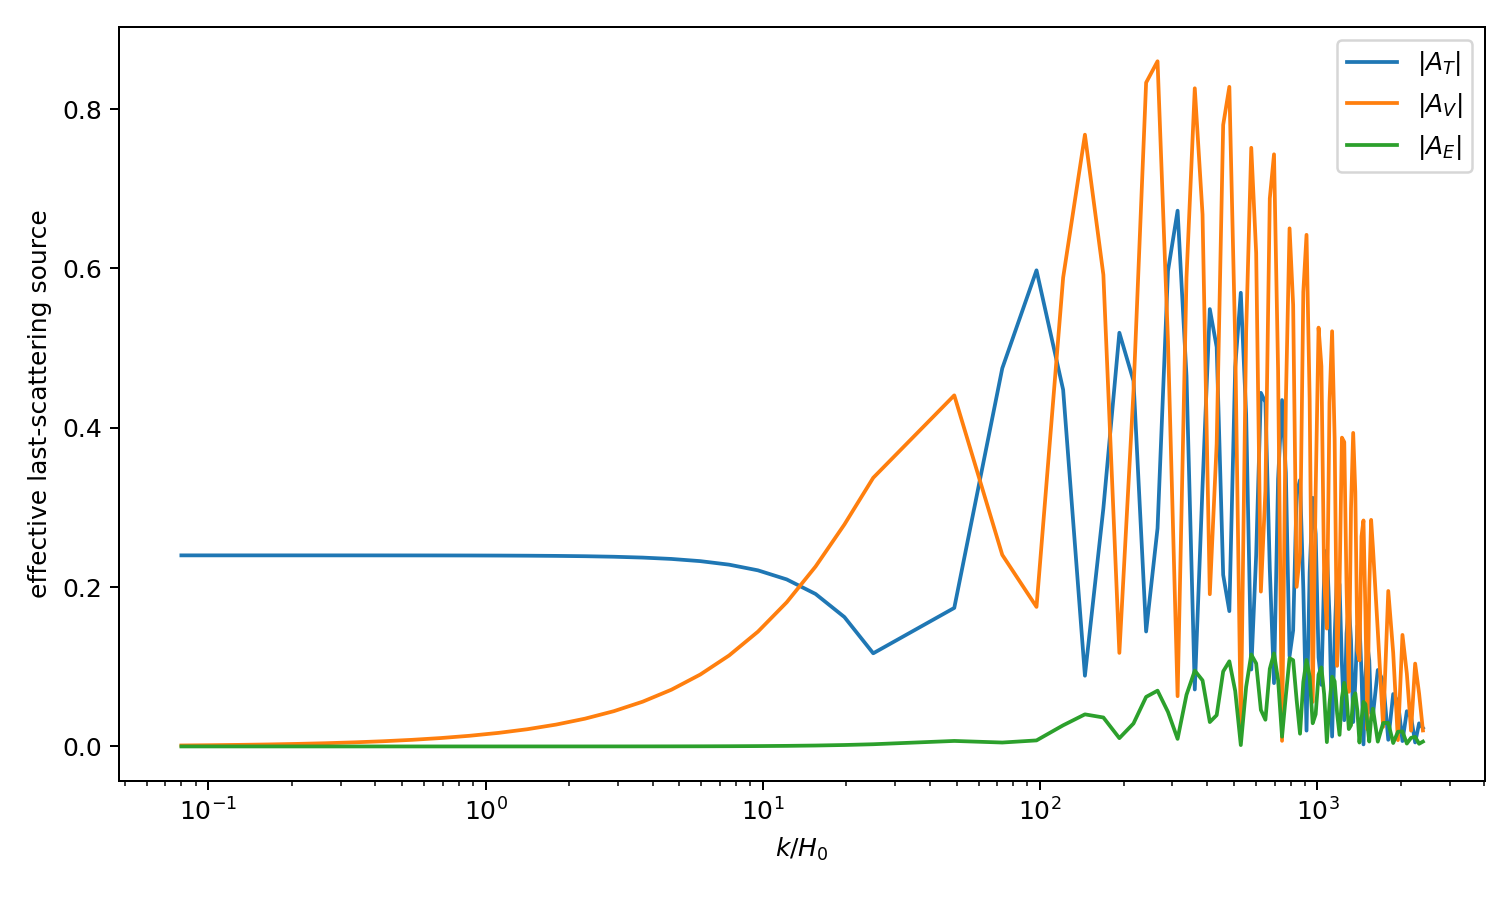
\includegraphics[width=0.88\linewidth]{figures/cmb/primary_cmb_sources.png}
\caption{Effective last-scattering temperature, velocity, and polarization source amplitudes.  The high-$k$ oscillations are sampled on the 101-mode Einstein--Boltzmann grid and spline-interpolated only at the final projection stage.}
\label{fig:pcmb-sources}
\end{figure}

\section{Finite-width last-scattering projection}

Define
\begin{equation}
 \Theta_0=\frac14F_{\gamma0}.
 \label{eq:pcmb-temperature-monopole}
\end{equation}
The source amplitudes in $dN$ measure are
\begin{equation}
 S_T
 =g_N\left(\Theta_0+\Psi+\frac1{16}\Pi_\gamma\right)
 +e^{-\tau}(\Psi_N-\Phi_N),
 \label{eq:pcmb-temperature-source}
\end{equation}
\begin{equation}
 S_V=g_N\frac{\theta_b}{k},
 \label{eq:pcmb-velocity-source}
\end{equation}
\begin{equation}
 S_E=\frac{3}{16}g_N\Pi_\gamma.
 \label{eq:pcmb-polarization-source}
\end{equation}
Their normalized integrated amplitudes are
\begin{equation}
 A_X(k)=\frac{1}{\mathcal R_\star}\int S_X(k,N)\,dN,
 \qquad
 X\in\{T,V,E\}.
 \label{eq:pcmb-integrated-sources}
\end{equation}

Let the visibility-weighted distance and width be
\begin{equation}
 \chi_\star
 =\frac{\int g_N\chi\,dN}{\int g_N\,dN},
 \qquad
 \sigma_\chi^2
 =\frac{\int g_N(\chi-\chi_\star)^2dN}{\int g_NdN}.
 \label{eq:pcmb-source-distance-width}
\end{equation}
The numerical values are
\begin{equation}
 \boxed{
 H_0\chi_\star=3.1438585561,
 \qquad
 H_0\sigma_\chi=2.3136123623\times10^{-3}.}
 \label{eq:pcmb-distance-width-values}
\end{equation}
The finite-width projection used here is
\begin{equation}
 \Delta_\ell^T(k)
 =e^{-k^2\sigma_\chi^2/2}
 \left[A_T(k)j_\ell(k\chi_\star)
 +A_V(k)j_\ell'(k\chi_\star)\right],
 \label{eq:pcmb-temperature-transfer}
\end{equation}
\begin{equation}
 \Delta_\ell^E(k)
 =e^{-k^2\sigma_\chi^2/2}
 \sqrt{\frac{(\ell+2)!}{(\ell-2)!}}
 A_E(k)\frac{j_\ell(k\chi_\star)}{(k\chi_\star)^2}.
 \label{eq:pcmb-e-transfer}
\end{equation}
This is a controlled narrow-source approximation.  A precision implementation would retain the complete time dependence inside the line-of-sight integral rather than compressing the source to $(A_T,A_V,A_E,\chi_\star,\sigma_\chi)$.

For
\begin{equation}
 \mathcal P_{\mathcal R}(k)
 =A_s\left(\frac{k}{k_\star}\right)^{n_s-1},
 \label{eq:pcmb-primordial-spectrum}
\end{equation}
with $A_s=2.1\times10^{-9}$, $n_s=0.965$, and $k_\star=0.05\,\mathrm{Mpc}^{-1}$, the angular spectra are
\begin{equation}
 C_\ell^{XY}
 =4\pi\int d\log k\,
 \mathcal P_{\mathcal R}(k)
 \Delta_\ell^X(k)\Delta_\ell^Y(k),
 \qquad
 X,Y\in\{T,E\}.
 \label{eq:pcmb-angular-spectra}
\end{equation}

\section{Acoustic and polarization results}

The visibility-peak sound horizon is
\begin{equation}
 H_0r_s=0.02913803155,
 \label{eq:pcmb-sound-horizon}
\end{equation}
and the geometric acoustic ruler is
\begin{equation}
 \boxed{
 \ell_A=\pi\frac{\chi_{\rm vis}}{r_s}=339.055741.}
 \label{eq:pcmb-acoustic-ruler}
\end{equation}
The first three resolved TT acoustic maxima above $\ell=80$ occur at
\begin{equation}
 \boxed{
 \ell_1=252,
 \qquad
 \ell_2=608,
 \qquad
 \ell_3=904.}
 \label{eq:pcmb-peak-positions}
\end{equation}
Their spacing is consistent with the geometric ruler to a relative discrepancy of $4.9975\times10^{-2}$ in the declared projection.

The first peak has
\begin{equation}
 \boxed{
 D_{\ell_1}^{TT}
 :=\frac{\ell_1(\ell_1+1)}{2\pi}C_{\ell_1}^{TT}T_{\gamma0}^2
 =6163.119890\,\mu\mathrm K^2.}
 \label{eq:pcmb-first-peak-amplitude}
\end{equation}
Selected template values are
\begin{center}
\begin{tabular}{rrrr}
\toprule
$\ell$ & $D_\ell^{TT}$ [$\mu$K$^2$] & $D_\ell^{EE}$ [$\mu$K$^2$] & $D_\ell^{TE}$ [$\mu$K$^2$]\\
\midrule
100 & 1220.174 & 0.289 & -1.418\\
200 & 4733.471 & 0.428 & -16.260\\
252 & 6163.120 & 0.459 & 17.919\\
500 & 2395.207 & 8.980 & -45.853\\
608 & 3467.906 & 4.787 & 27.666\\
904 & 3099.722 & 9.410 & -46.574\\
1000 & 1904.695 & 11.920 & 58.657\\
1500 & 343.904 & 15.671 & -25.350\\
2000 & 138.183 & 1.915 & 2.085\\
2500 & 10.197 & 1.762 & -0.480\\
\bottomrule
\end{tabular}
\end{center}
The temperature--polarization cross spectrum satisfies the Cauchy bound over every stored multipole,
\begin{equation}
 \max_\ell\frac{|C_\ell^{TE}|}{\sqrt{C_\ell^{TT}C_\ell^{EE}}}
 =0.9948225265<1.
 \label{eq:pcmb-te-cauchy}
\end{equation}

\begin{figure}[htbp]
\centering
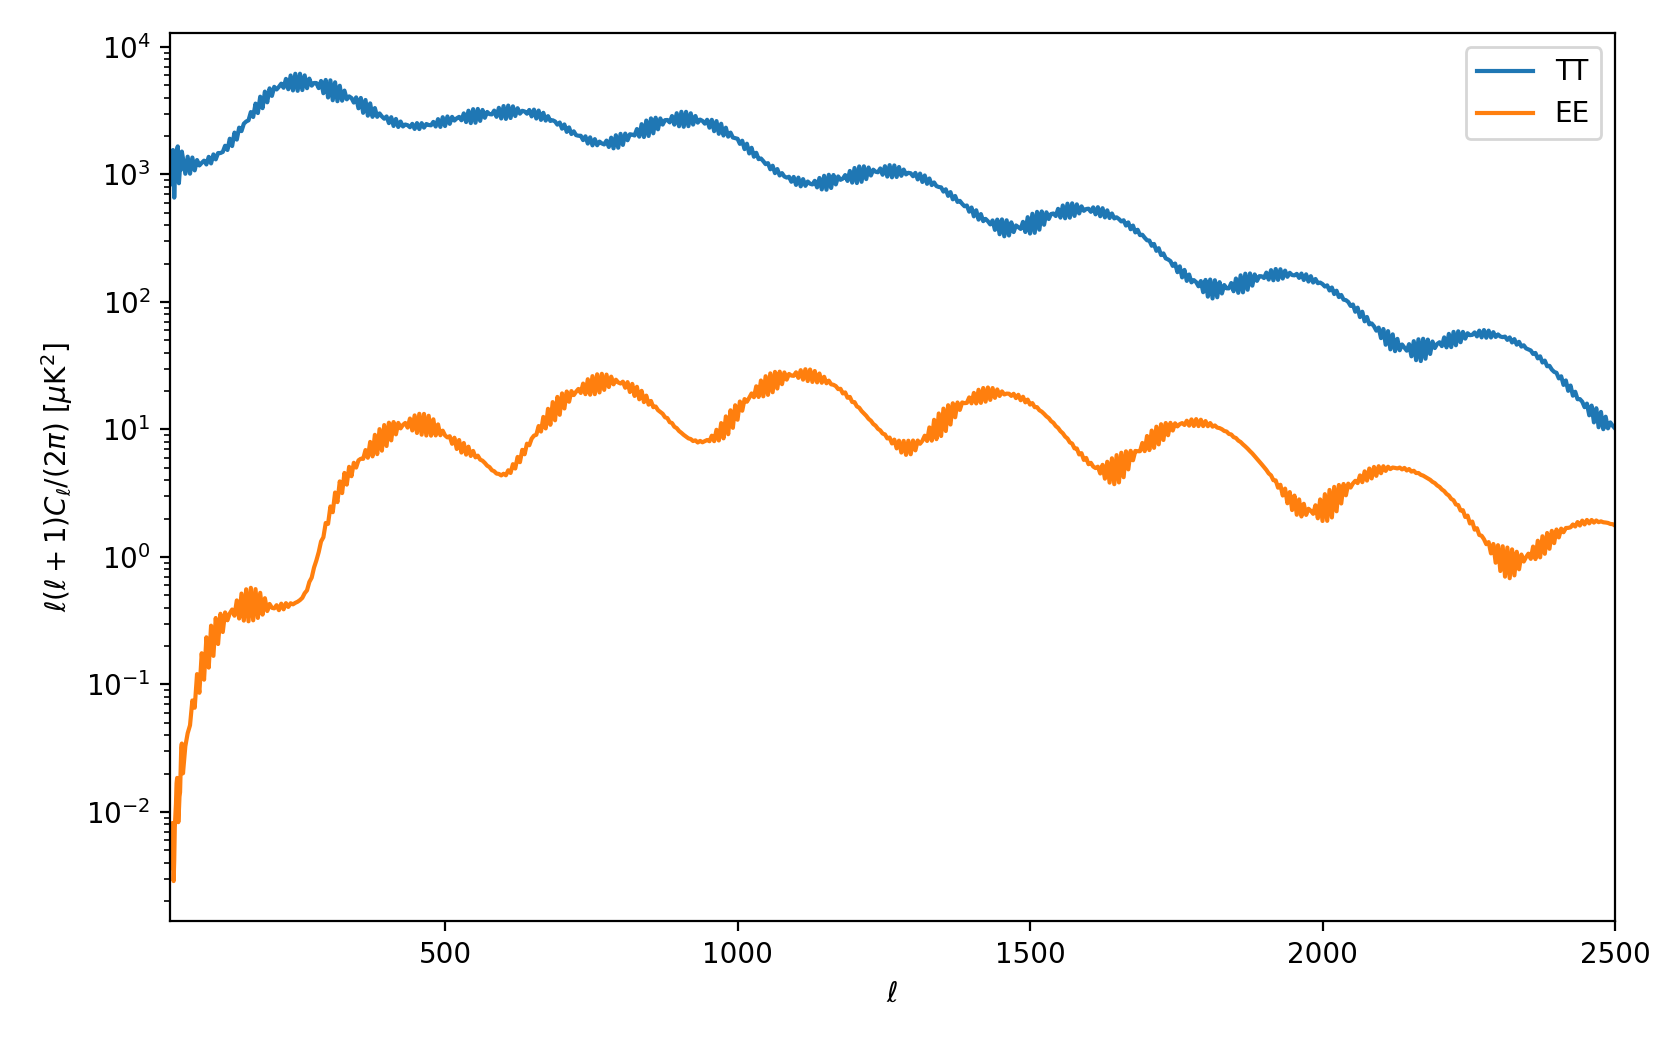
\includegraphics[width=0.90\linewidth]{figures/cmb/primary_cmb_tt_ee_acoustic.png}
\caption{Controlled recombination-era TT and EE templates.  The plotted range begins at $\ell=30$ because reionization and late integrated sources are not included.}
\label{fig:pcmb-tt-ee}
\end{figure}

\begin{figure}[htbp]
\centering
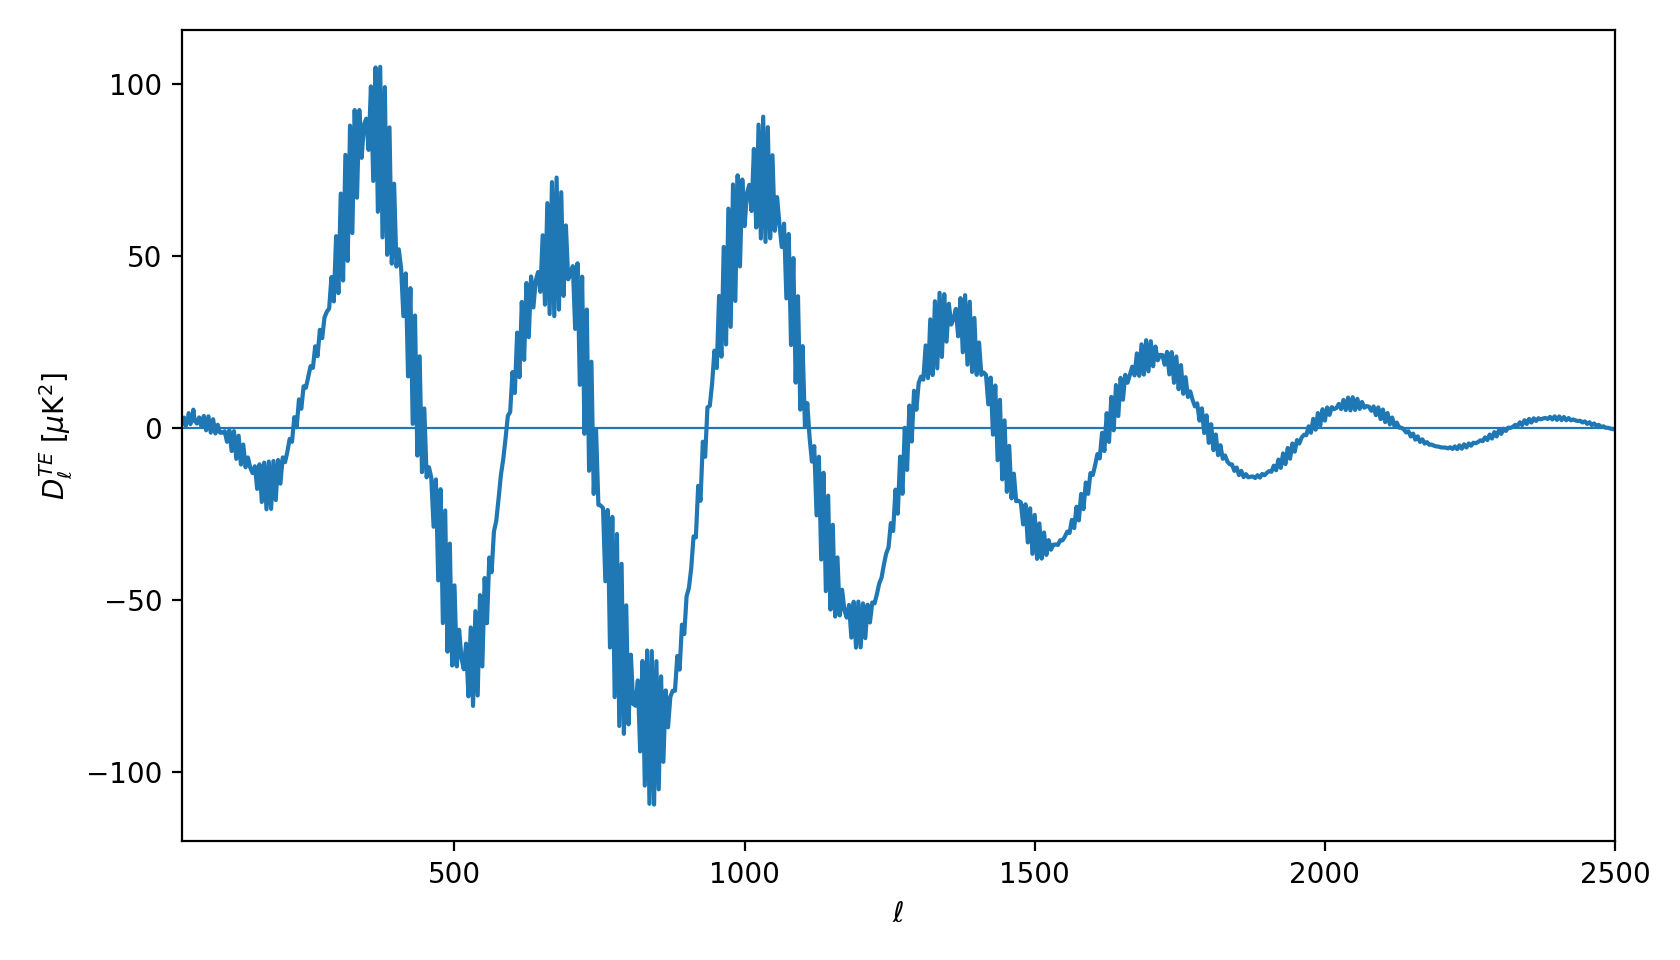
\includegraphics[width=0.90\linewidth]{figures/cmb/primary_cmb_te_acoustic.png}
\caption{The controlled TE template alternates sign across the acoustic series, reflecting the relative phase of photon compression, velocity, and polarization.}
\label{fig:pcmb-te}
\end{figure}

The finite source width suppresses high multipoles.  At $\ell=3000$, the declared Gaussian thickness factor is
\begin{equation}
 \exp\left[-\frac12
 \left(\frac{\ell\sigma_\chi}{\chi_\star}\right)^2\right]_{\ell=3000}
 =0.08741675187.
 \label{eq:pcmb-thickness-factor}
\end{equation}

\section{Convergence and verification}

The main deterministic audit contains
\begin{equation}
 \boxed{
 20\ \mathrm{PASS},
 \qquad
 0\ \mathrm{FAIL}.}
 \label{eq:pcmb-main-checks}
\end{equation}
A separate convergence audit adds
\begin{equation}
 \boxed{
 4\ \mathrm{PASS},
 \qquad
 0\ \mathrm{FAIL}.}
 \label{eq:pcmb-convergence-checks}
\end{equation}
The combined calculation therefore records
\begin{equation}
 \boxed{
 24\ \mathrm{PASS},
 \qquad
 0\ \mathrm{FAIL}.}
 \label{eq:pcmb-total-checks}
\end{equation}
The principal refinement differences are
\begin{center}
\begin{tabular}{lr}
\toprule
control & relative discrepancy\\
\midrule
momentum quadrature & $1.81645\times10^{-4}$\\
photon--neutrino--dark multipole truncation & $6.48202\times10^{-3}$\\
time step & $2.19752\times10^{-6}$\\
accepted-state Einstein constraint & $1.20910\times10^{-4}$\\
\bottomrule
\end{tabular}
\end{center}
The free-streaming spherical-Bessel identity is reproduced with maximum residual
\begin{equation}
 \epsilon_{\rm fs}=1.35046\times10^{-6}
 \label{eq:pcmb-free-streaming-residual}
\end{equation}
in the finite-difference derivative audit.  Median held-out source-interpolation errors are
\begin{equation}
 \epsilon_{A_T}=1.38235\times10^{-2},
 \qquad
 \epsilon_{A_V}=1.45514\times10^{-2},
 \qquad
 \epsilon_{A_E}=1.42026\times10^{-2}.
 \label{eq:pcmb-source-interpolation-errors}
\end{equation}
These source errors, together with the narrow-source projection, dominate over the time-step and momentum-quadrature errors in the current spectra.

\section{Closure ledger}

\begin{center}
\begin{tabular}{>{\raggedright\arraybackslash}p{0.47\linewidth}>{\raggedright\arraybackslash}p{0.21\linewidth}>{\raggedright\arraybackslash}p{0.24\linewidth}}
\toprule
statement & status & boundary\\
\midrule
photon temperature hierarchy with Thomson scattering & closed controlled & scalar linear perturbations\\
scalar polarization hierarchy and nonzero $E$ source & closed controlled & no $B$ modes\\
baryon drag and acoustic loading & closed controlled & simple baryon thermal history\\
massless-neutrino hierarchy and anisotropic stress & closed controlled & fixed $\Omega_{\nu0}$\\
massive refinement hierarchy through recombination & closed controlled & seven levels, fourteen phase nodes\\
Einstein momentum and shear coupling & closed controlled & Newtonian gauge\\
energy-constraint audit & numerically controlled & not projected after each step\\
Saha visibility and finite source width & closed conditional & no multilevel recombination\\
recombination-era TT, TE, EE acoustic templates & numerically closed & narrow-source projection\\
low-$\ell$ TT, TE, EE prediction & open & reionization and late integrated sources\\
precision recombination and helium kinetics & open & external atomic network\\
full line-of-sight source integration & open & production-grade transfer solver\\
lensing remapping and nonlinear late-time sources & open & nonlinear structure\\
joint likelihood and parameter inference & open & observational data and nuisance model\\
microscopic perturbation matching at production & open & nonlinear inhomogeneous crossing\\
\bottomrule
\end{tabular}
\end{center}

\clearpage
\section{Synthesis and scope}

The scale-covariant distribution now enters one coupled chain,
\begin{equation}
 \boxed{
 \begin{gathered}
 \bar f_h(q)
 \longrightarrow
 \{F_{h\ell},F_{\nu\ell},F_{\gamma\ell},G_{\gamma\ell},\delta_b,\theta_b\}
 \\
 \longrightarrow
 \{\Phi,\Psi,g_N\}
 \longrightarrow
 \{A_T,A_V,A_E\}
 \longrightarrow
 \{C_\ell^{TT},C_\ell^{TE},C_\ell^{EE}\}.
 \end{gathered}}
 \label{eq:pcmb-result-chain}
\end{equation}
No dark-sector parameter is changed between production, background expansion, late-time collisionless structure, and the controlled primary-CMB calculation.

This closes the principal species-coupling gap at the level of a deterministic linear template.  A precision line-of-sight and thermal-history treatment still requires:
\begin{equation}
 \boxed{
 \begin{gathered}
 \text{replace Saha recombination by multilevel H/He kinetics},\\
 \text{derive the production-surface perturbation transfer},\\
 \text{add reionization, late ISW, and lensing remapping},\\
 \text{compute primary and late-time observables in one solver},\\
 \text{then perform a first joint likelihood without dark-sector retuning}.
 \end{gathered}}
 \label{eq:pcmb-open-requirements}
\end{equation}
\chapter{Effective Thermal History, Production-Surface Matching, Reionization, and Late-Time Line-of-Sight Closure}
\label{ch:thermal-reionization-los}

\section{Scope and objective}

The preceding production-to-primary-CMB calculation jointly evolved photons, scalar polarization, baryons, massless neutrinos, metric perturbations, and the massive refinement hierarchy through a controlled recombination surface.  Its stated thermal and projection limitations were Saha hydrogen recombination, no reionization, no late integrated Sachs--Wolfe source, and a narrow finite-width last-scattering projection.  This chapter extends that framework by adding
\begin{equation}
\boxed{
\begin{gathered}
\text{effective Peebles hydrogen recombination}
+\text{ controlled helium transitions}\\
+\text{ optical-depth-calibrated reionization}
+\text{ single-clock production matching}\\
+\text{ finite-width recombination and reionization projection}
+\text{ time-resolved late ISW transport}.
\end{gathered}}
\label{eq:trl-objective}
\end{equation}
The early acoustic source amplitudes are inherited from the coupled Einstein--Boltzmann solve without dark-sector retuning.  The new calculation is a controlled thermal-history and late-source closure.  It is not a precision recombination code, an astrophysical reionization prediction, or a likelihood analysis.

A sign correction is also made.  In the Newtonian-gauge convention used here, the integrated temperature source is proportional to
\begin{equation}
\Phi'+\Psi',
\label{eq:trl-isw-sum}
\end{equation}
not to their difference.  The corrected sum is used throughout this chapter.

\section{Unchanged cosmological and refinement input}

Use
\begin{equation}
E(a)^2
=
\Omega_{r0}a^{-4}
+\Omega_{m0}a^{-3}
+\Omega_{V0},
\qquad
\Omega_{m0}=\Omega_{b0}+\Omega_{D0},
\label{eq:trl-background}
\end{equation}
with
\begin{equation}
\Omega_{b0}=0.049,
\qquad
\Omega_{D0}=0.261,
\qquad
\Omega_{r0}=9\times10^{-5},
\qquad
\Omega_{V0}=1-\Omega_{m0}-\Omega_{r0}.
\label{eq:trl-fractions}
\end{equation}
The conditional physical conversion uses
\begin{equation}
H_0=70\ {\rm km\,s^{-1}\,Mpc^{-1}},
\qquad
T_{\gamma0}=2.7255\ {
m K},
\qquad
Y_p=0.24.
\label{eq:trl-conventions}
\end{equation}
The primordial spectrum remains
\begin{equation}
\mathcal P_{\mathcal R}(k)
=A_s\left(\frac{k}{k_\star}\right)^{n_s-1},
\qquad
A_s=2.1\times10^{-9},
\qquad
n_s=0.965,
\qquad
k_\star=0.05\ {\rm Mpc}^{-1}.
\label{eq:trl-primordial}
\end{equation}
The recombination-era acoustic source functions
\begin{equation}
A_T(k),\qquad A_V(k),\qquad A_E(k)
\label{eq:trl-parent-sources}
\end{equation}
are read directly from the preceding coupled solve.  No parameter of the scale-covariant dark sector is refitted in this calculation.

\section{Effective Peebles hydrogen recombination}

Let
\begin{equation}
N=\log a,
\qquad
T_\gamma=\frac{T_{\gamma0}}{a},
\qquad
n_H(a)=n_{H0}a^{-3}.
\label{eq:trl-recomb-definitions}
\end{equation}
The case-B coefficient is represented by the controlled fit
\begin{equation}
\alpha_B(T)
=
4.309\times10^{-19}
\frac{t^{-0.6166}}{1+0.6703t^{0.5300}}
\ {\rm m^3\,s^{-1}},
\qquad
t=\frac{T}{10^4\ {\rm K}}.
\label{eq:trl-alphaB}
\end{equation}
Detailed balance gives
\begin{equation}
\beta_B(T)
=
\alpha_B(T)
\left(\frac{m_ek_BT}{2\pi\hbar^2}\right)^{3/2}
\exp\left(-\frac{E_2}{k_BT}\right),
\qquad
E_2=3.4\ {\rm eV}.
\label{eq:trl-betaB}
\end{equation}
Define
\begin{equation}
K_\alpha
=
\frac{\lambda_\alpha^3}{8\pi H},
\qquad
C_P
=
\frac{1+K_\alpha\Lambda_{2s}n_H(1-x_H)}
{1+K_\alpha(\Lambda_{2s}+\beta_B)n_H(1-x_H)}.
\label{eq:trl-peebles-C}
\end{equation}
The effective three-level hydrogen equation is
\begin{equation}
\boxed{
\frac{dx_H}{dN}
=
\frac{C_P}{H}
\left[
\beta_B(1-x_H)
\exp\left(-\frac{E_\alpha}{k_BT}\right)
-n_H\alpha_Bx_H^2
\right],
}
\label{eq:trl-peebles-eq}
\end{equation}
where
\begin{equation}
E_\alpha=10.2\ {\rm eV},
\qquad
\Lambda_{2s}=8.22458\ {\rm s}^{-1},
\qquad
\lambda_\alpha=121.567\ {\rm nm}.
\label{eq:trl-atomic-constants}
\end{equation}
The calculation follows the Saha solution until
\begin{equation}
x_H\simeq0.99,
\qquad
z\simeq1577.09,
\label{eq:trl-switch}
\end{equation}
and then integrates \eqref{eq:trl-peebles-eq}.  It gives
\begin{equation}
\boxed{x_{H,{\rm residual}}=2.8029283896\times10^{-4}.}
\label{eq:trl-residual-xe}
\end{equation}

The helium contribution is represented by controlled smooth transitions for HeIII-to-HeII and HeII-to-HeI.  This preserves the correct electron-counting limits but is not a multilevel helium-kinetics calculation.

\section{Reionization and optical-depth calibration}

Let
\begin{equation}
y(z)=(1+z)^{3/2}.
\label{eq:trl-yre}
\end{equation}
The hydrogen reionization fraction is modeled by
\begin{equation}
R_H(z)
=
\frac12
\left[
1+\tanh\left(
\frac{y(z_{\rm re})-y(z)}{\Delta y_{\rm re}}
\right)
\right],
\label{eq:trl-tanh-reionization}
\end{equation}
with
\begin{equation}
\Delta y_{\rm re}
=
\frac32\sqrt{1+z_{\rm re}}\,\Delta z_{\rm re},
\qquad
\Delta z_{\rm re}=0.5.
\label{eq:trl-dyre}
\end{equation}
A second smooth transition accounts for the late second helium ionization.

The optical-depth equation in logarithmic scale factor is
\begin{equation}
\frac{d\tau}{dN}
=
\frac{n_e\sigma_Tc}{H},
\label{eq:trl-tau}
\end{equation}
and the visibility per unit $N$ is
\begin{equation}
g_N(N)
=
\exp[-\tau(N)]\frac{d\tau}{dN}.
\label{eq:trl-visibility}
\end{equation}
The reionization midpoint is fixed by the declared input
\begin{equation}
\tau_{\rm re}=0.054.
\label{eq:trl-tau-target}
\end{equation}
The calibrated result is
\begin{equation}
\boxed{z_{\rm re}=7.4124651067,}
\qquad
\boxed{z_{g,{\rm re}}=6.6559660691.}
\label{eq:trl-zre-results}
\end{equation}
The total visibility satisfies
\begin{equation}
\boxed{
\int g_N\,dN
=0.9999979519.
}
\label{eq:trl-visibility-normalization}
\end{equation}
The recombination and reionization pieces carry
\begin{equation}
\int g_{N,{\rm rec}}\,dN=0.9474304116,
\qquad
\int g_{N,{\rm re}}\,dN=0.0525675402.
\label{eq:trl-vis-split}
\end{equation}

\begin{figure}[htbp]
\centering
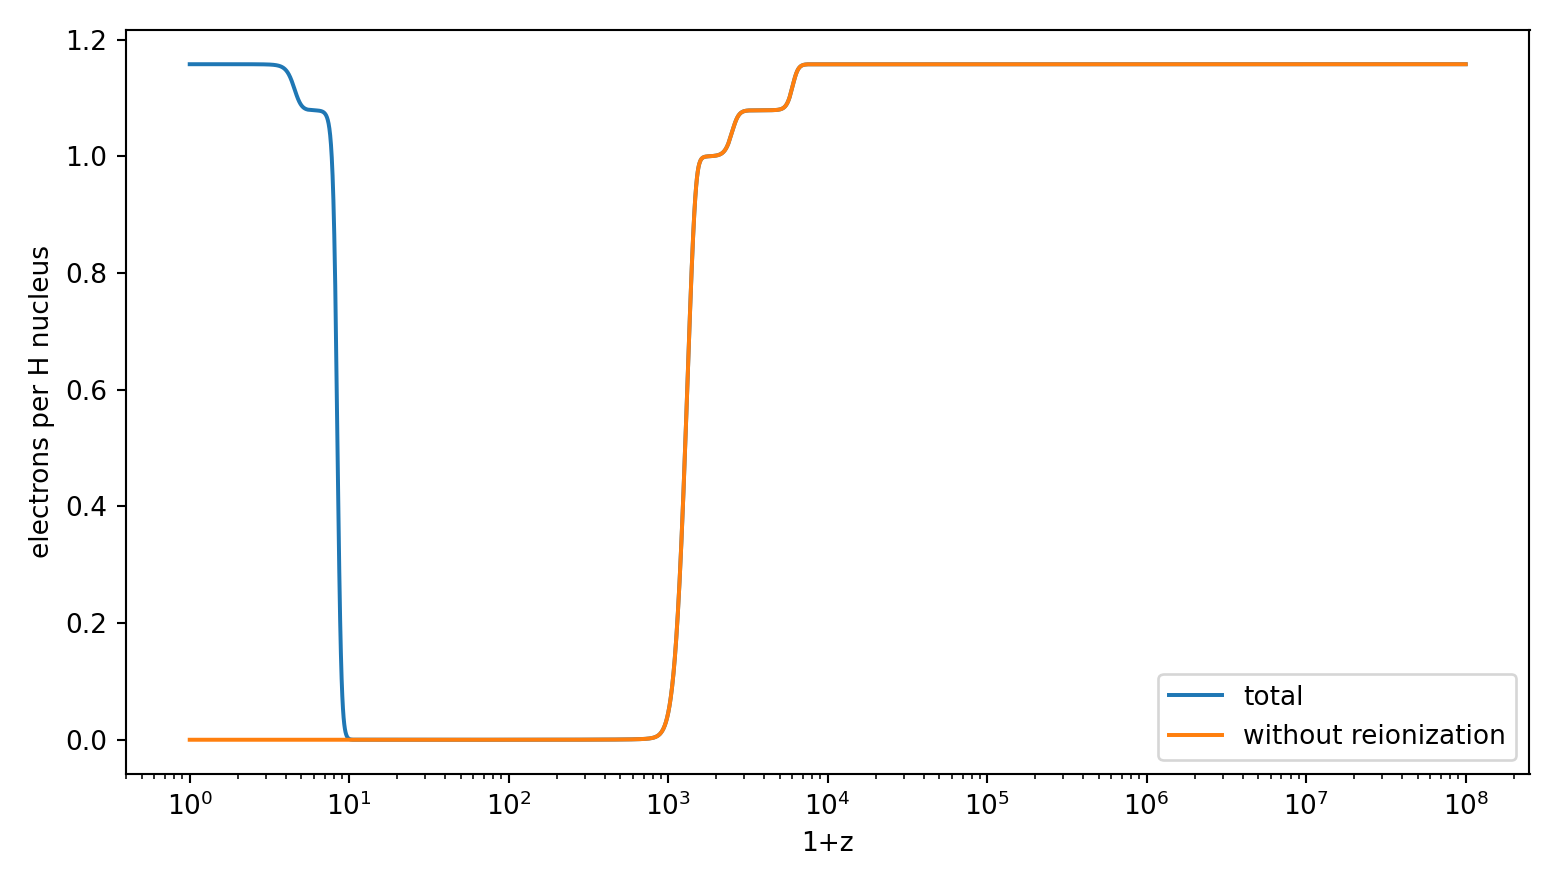
\includegraphics[width=0.86\linewidth]{figures/los/effective_ionization_history.png}
\caption{Effective hydrogen-plus-helium ionization history before and after the optical-depth-calibrated reionization transition.}
\label{fig:trl-ionization}
\end{figure}

\begin{figure}[htbp]
\centering
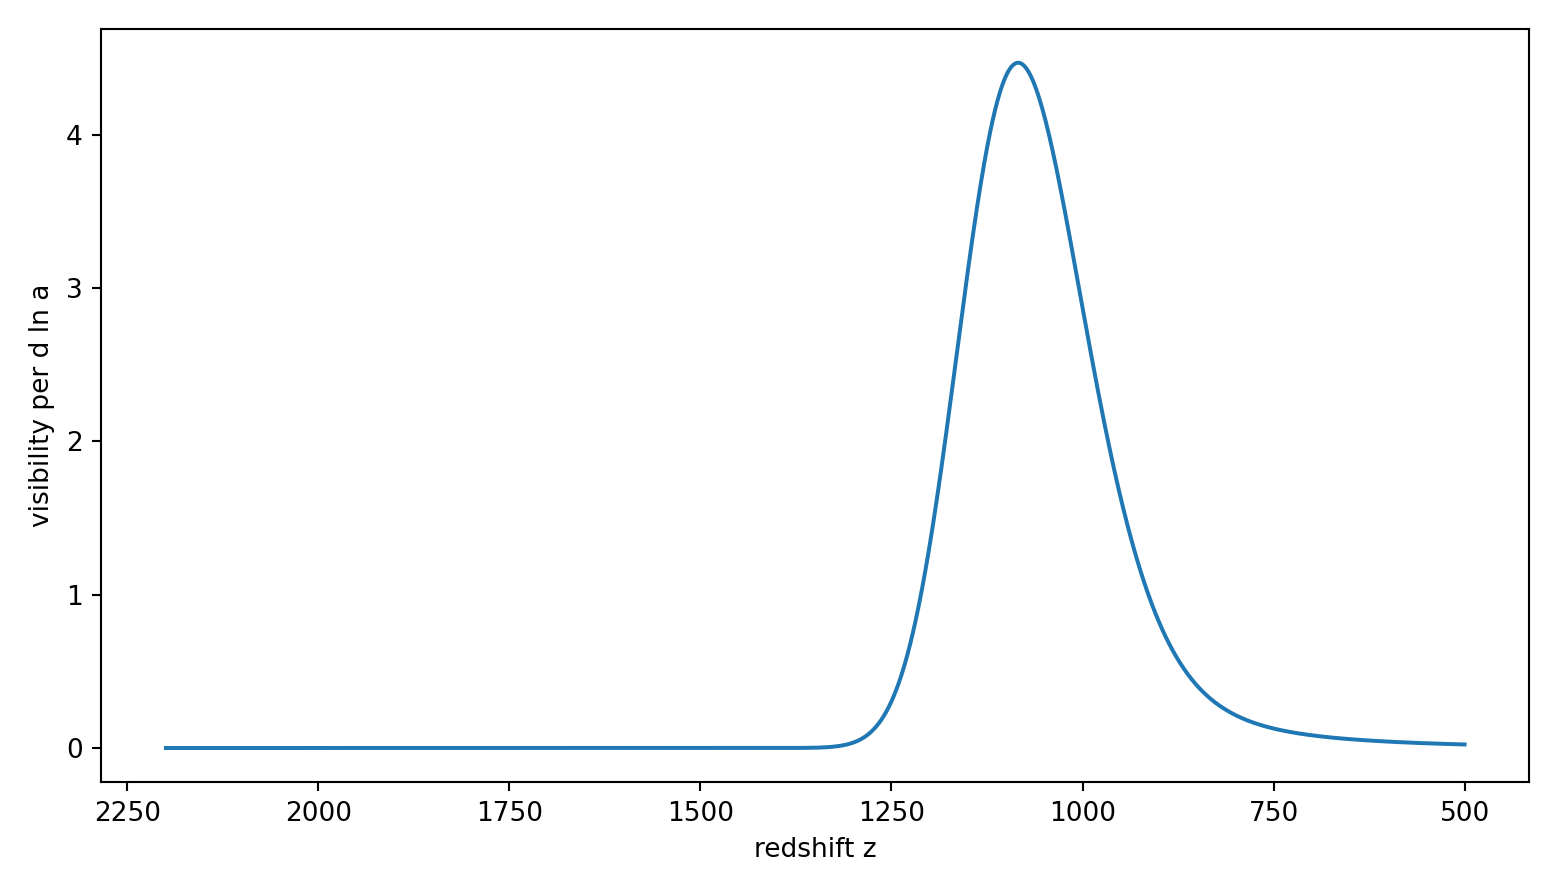
\includegraphics[width=0.82\linewidth]{figures/los/effective_recombination_visibility.png}
\caption{Effective recombination visibility.  The peak shifts from the preceding Saha benchmark to the controlled Peebles value near $z=1084$.}
\label{fig:trl-recombination-vis}
\end{figure}

\begin{figure}[htbp]
\centering
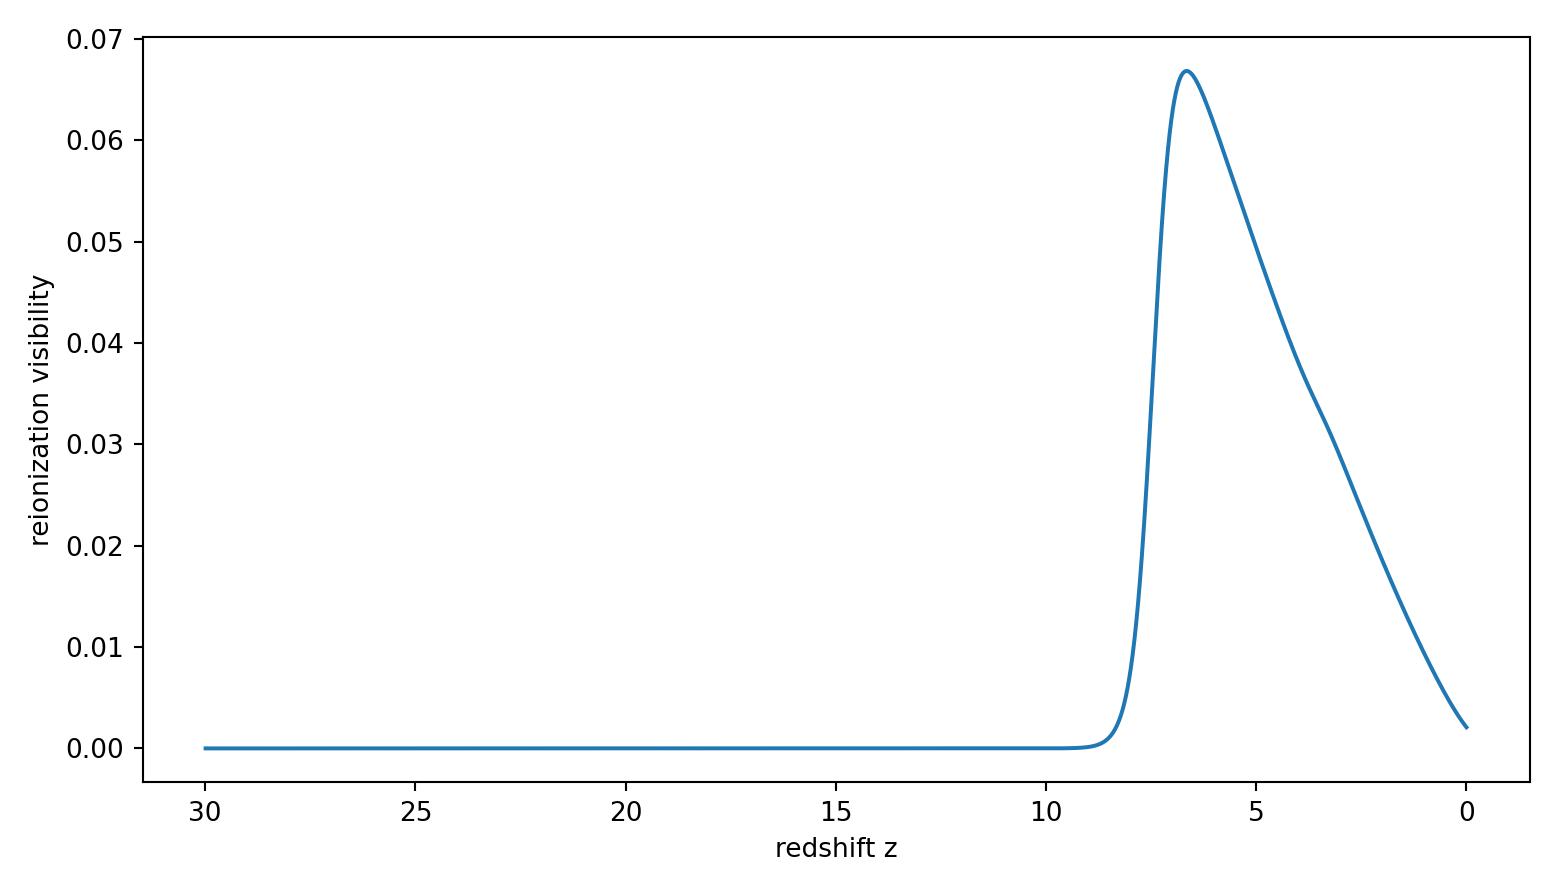
\includegraphics[width=0.82\linewidth]{figures/los/reionization_visibility.png}
\caption{Reionization-only visibility after subtracting the recombination history.}
\label{fig:trl-reionization-vis}
\end{figure}

\section{Visibility moments and finite-thickness projection}

For a nonnegative source weight $w(N)$, define
\begin{equation}
\mathcal N_w=\int w\,dN,
\qquad
\chi_w=\frac{1}{\mathcal N_w}\int w\chi\,dN,
\label{eq:trl-shell-mean}
\end{equation}
\begin{equation}
\sigma_{\chi,w}^2
=
\frac{1}{\mathcal N_w}
\int w(\chi-\chi_w)^2\,dN.
\label{eq:trl-shell-rms}
\end{equation}
The long residual-ionization tail makes the global recombination RMS width a poor Gaussian approximation to the acoustic core.  The calculation therefore archives the full visibility and both widths, while the acoustic thickness factor uses the FWHM-equivalent central width
\begin{equation}
\sigma_{\chi,{\rm core}}
=
\frac{\Delta\chi_{\rm FWHM}}{2\sqrt{2\log2}}.
\label{eq:trl-core-width}
\end{equation}
The measured quantities are
\begin{equation}
\boxed{
\chi_{\rm rec}=3.1335298685\ H_0^{-1},
\qquad
\sigma_{\chi,{\rm core}}=3.7505054558\times10^{-3}\ H_0^{-1},
}
\label{eq:trl-rec-shell}
\end{equation}
\begin{equation}
\sigma_{\chi,{\rm RMS}}=1.6282448527\times10^{-2}\ H_0^{-1},
\label{eq:trl-rec-rms}
\end{equation}
\begin{equation}
\boxed{
\chi_{\rm re}=1.5792968823\ H_0^{-1},
\qquad
\sigma_{\chi,{\rm re}}=0.4275528337\ H_0^{-1}.
}
\label{eq:trl-re-shell}
\end{equation}
The recombination visibility peaks at
\begin{equation}
\boxed{z_{\rm rec}=1084.47305577.}
\label{eq:trl-zrec}
\end{equation}

\section{Single-clock production-surface matching}

Let the production hypersurface be defined by one local clock $F$,
\begin{equation}
F(t,\boldsymbol x)=F_\star.
\label{eq:trl-production-surface}
\end{equation}
At first perturbative order, its displacement is
\begin{equation}
\delta t_\star
=-\frac{\delta F}{\dot{\bar F}}.
\label{eq:trl-deltat}
\end{equation}
Suppose every produced refinement level depends on the same clock and no independent modulation field is present.  Then
\begin{equation}
\delta\rho_h
=-\dot{\bar\rho}_h\,\delta t_\star.
\label{eq:trl-density-matching}
\end{equation}
The curvature perturbation of each level is
\begin{equation}
\zeta_h
=-\Phi-H\frac{\delta\rho_h}{\dot{\bar\rho}_h}
=-\Phi+H\delta t_\star,
\label{eq:trl-zeta-level}
\end{equation}
so that
\begin{equation}
\boxed{
S_{hj}:=3(\zeta_h-\zeta_j)=0.
}
\label{eq:trl-zero-isocurvature}
\end{equation}
Thus a single-clock crossing supplies adiabatic production-surface matching at leading gradient order.

An independent modulation $A_\star(\boldsymbol x)$ generates a calculable entropy direction.  For
\begin{equation}
n_h
\propto
\nu_h^{3/2}
\exp\left(-\frac{\pi m_h^2}{\nu_h}\right),
\qquad
\nu_h=A_\star m_h,
\label{eq:trl-number-spectrum}
\end{equation}
its response is
\begin{equation}
\boxed{
\frac{\partial\log n_h}{\partial\log A_\star}
=
\frac32+\frac{\pi m_h}{A_\star}.
}
\label{eq:trl-modulation-response}
\end{equation}
This distinguishes the adiabatic single-clock prediction from an independently modulated production event.

\begin{figure}[htbp]
\centering
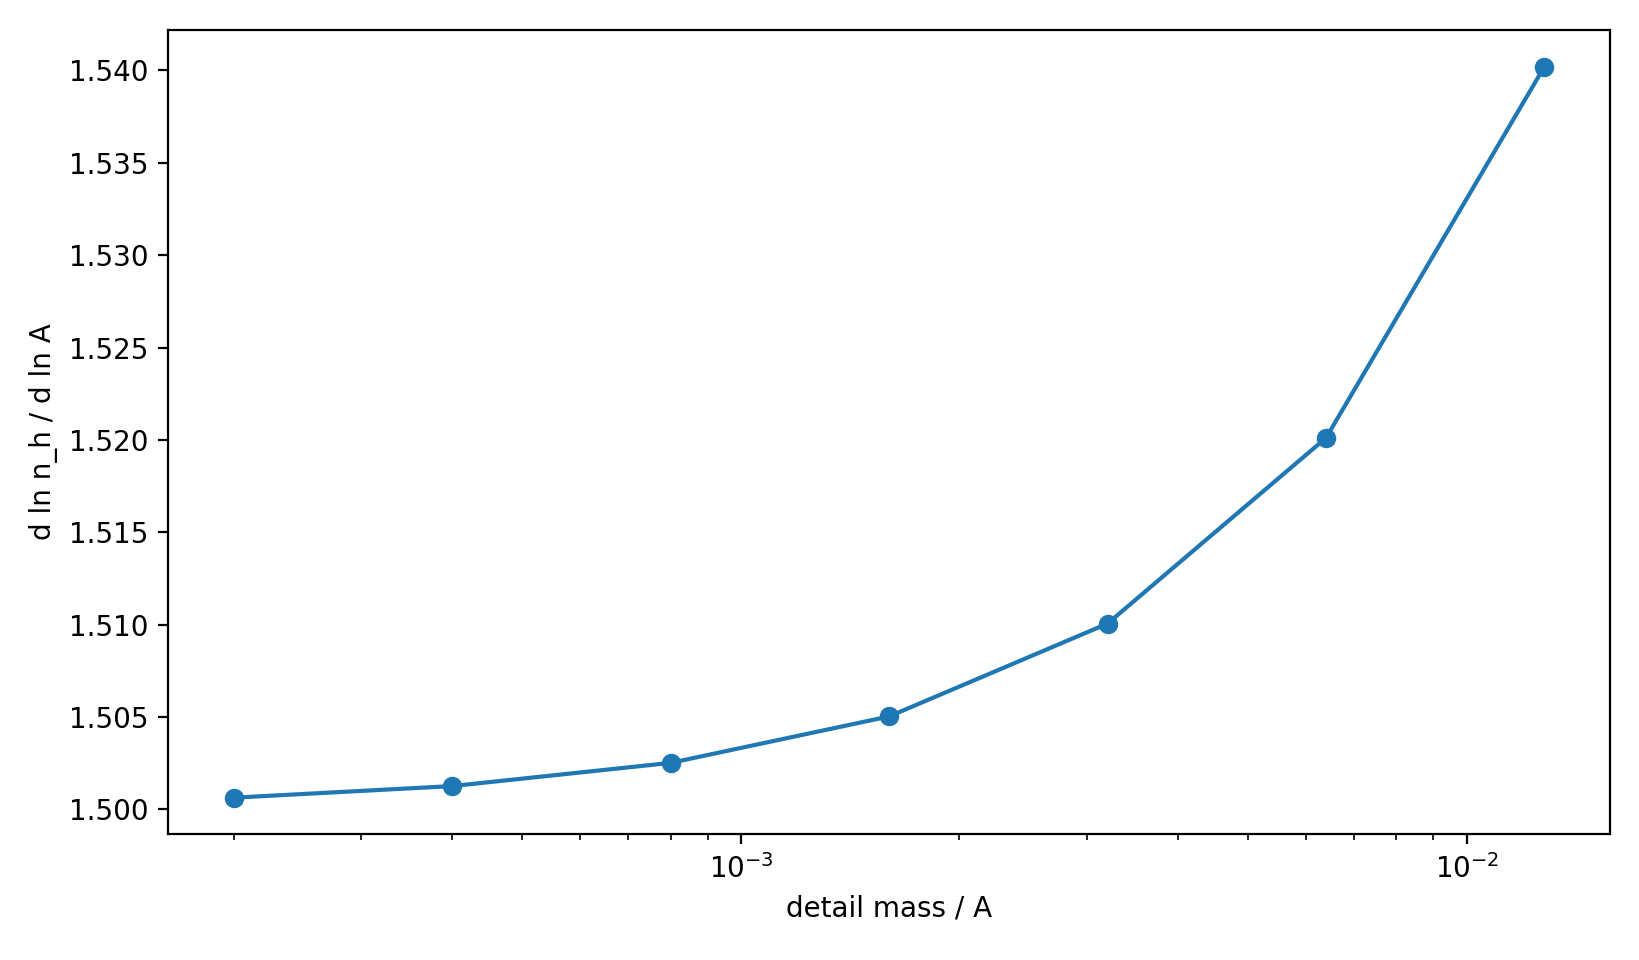
\includegraphics[width=0.80\linewidth]{figures/los/production_modulation_response.png}
\caption{Level-dependent abundance response to an independent production-scale modulation.  The single-clock relative entropy remains zero; the plotted response applies only to an additional modulation direction.}
\label{fig:trl-production-response}
\end{figure}

\section{Corrected line-of-sight source}

Use Newtonian gauge
\begin{equation}
ds^2
=a^2(\eta)
\left[-(1+2\Psi)d\eta^2+(1-2\Phi)d\boldsymbol x^2\right].
\label{eq:trl-newtonian-gauge}
\end{equation}
For the collisionless temperature brightness after the standard gravitational redshift rearrangement,
\begin{equation}
(\Theta+\Psi)'
+ik\mu(\Theta+\Psi)
=
\Phi'+\Psi'+\mathcal C_\gamma.
\label{eq:trl-los-eq}
\end{equation}
Therefore the late integrated source is
\begin{equation}
\boxed{
S_{\rm ISW}=e^{-\tau}(\Phi'+\Psi').
}
\label{eq:trl-isw-source}
\end{equation}
The earlier difference source is superseded in this convention.

Let
\begin{equation}
\mathcal T_\ell(k)
=\mathcal T_{\ell,{\rm rec}}(k)
+\mathcal T_{\ell,{\rm re}}(k)
+\mathcal T_{\ell,{\rm ISW}}(k).
\label{eq:trl-total-transfer}
\end{equation}
The finite-width recombination term is
\begin{equation}
\mathcal T_{\ell,{\rm rec}}
=e^{-\tau_{\rm re}}
\exp\left(-\frac{k^2\sigma_{\chi,{\rm core}}^2}{2}\right)
\left[
A_T(k)j_\ell(k\chi_{\rm rec})
+A_V(k)j_\ell'(k\chi_{\rm rec})
\right].
\label{eq:trl-rec-transfer}
\end{equation}
Free streaming from recombination to the effective reionization shell reconstructs
\begin{equation}
\Theta_0^{\rm re}(k)
=A_Tj_0(k\Delta\chi)+A_Vj_0'(k\Delta\chi),
\label{eq:trl-reion-monopole}
\end{equation}
\begin{equation}
\Theta_2^{\rm re}(k)
=A_Tj_2(k\Delta\chi)+A_Vj_2'(k\Delta\chi),
\qquad
\Pi_{\rm re}=4\Theta_2^{\rm re},
\label{eq:trl-reion-quadrupole}
\end{equation}
where
\begin{equation}
\Delta\chi=\chi_{\rm rec}-\chi_{\rm re}.
\label{eq:trl-deltachi}
\end{equation}
The reionization temperature and polarization sources are then projected with the measured reionization width.

The late potential is evolved with
\begin{equation}
D_{NN}
+\left(2+\frac{d\log H}{dN}\right)D_N
-\frac32\Omega_m(a)D=0,
\label{eq:trl-growth}
\end{equation}
\begin{equation}
g_\Phi(a)=\frac{D(a)}{a},
\qquad
\Phi=\Psi=\frac35\mathcal R\,T(k)g_\Phi(a),
\label{eq:trl-potential-growth}
\end{equation}
which gives the time-resolved integral
\begin{equation}
\mathcal T_{\ell,{\rm ISW}}(k)
=
\int dN\,
2e^{-\tau}
\frac{d\Phi}{dN}
 j_\ell[k\chi(N)].
\label{eq:trl-isw-integral}
\end{equation}
The $E$-mode transfer is constructed from the recombination and reionization quadrupole sources with the scalar spin-2 projection factor
\begin{equation}
\sqrt{\frac{(\ell+2)!}{(\ell-2)!}}
\frac{j_\ell(x)}{x^2}.
\label{eq:trl-spin2}
\end{equation}
Finally,
\begin{equation}
\boxed{
C_\ell^{XY}
=4\pi\int d\log k\,
\mathcal P_{\mathcal R}(k)
\mathcal T_\ell^X(k)
\mathcal T_\ell^Y(k),
\qquad
X,Y\in\{T,E\}.
}
\label{eq:trl-cl}
\end{equation}

\section{Acoustic ruler and controlled spectra}

The effective sound horizon is
\begin{equation}
r_s
=\int^{N_{\rm rec}}
\frac{dN}{\mathcal H\sqrt{3(1+R_b)}},
\qquad
R_b=\frac{3\rho_b}{4\rho_\gamma}.
\label{eq:trl-rs}
\end{equation}
The calculation gives
\begin{equation}
\boxed{H_0r_s=0.03280490608,}
\qquad
\boxed{\ell_A=\frac{\pi\chi_{\rm rec}}{r_s}=300.0854321.}
\label{eq:trl-acoustic-ruler}
\end{equation}
The first three resolved temperature maxima above $\ell=150$ occur at
\begin{equation}
\boxed{
\ell_1=262,
\qquad
\ell_2=582,
\qquad
\ell_3=894.
}
\label{eq:trl-peaks}
\end{equation}
The first peak amplitude is
\begin{equation}
\boxed{D_{262}^{TT}=4063.713734\ \mu{\rm K}^2.}
\label{eq:trl-first-peak}
\end{equation}

\begin{table}[htbp]
\centering
\small
\begin{tabular}{rrrr}
\toprule
$\ell$ & $D_\ell^{TT}$ [$\mu{\rm K}^2$] & $D_\ell^{EE}$ [$\mu{\rm K}^2$] & $D_\ell^{TE}$ [$\mu{\rm K}^2$]\\
\midrule
2    & 316.421 & 0.03564 & 1.6379\\
5    & 317.116 & 0.00992 & 0.9739\\
10   & 396.325 & 0.00006 & 0.1210\\
50   & 977.218 & 0.02039 & 1.2588\\
100  & 1279.639 & 0.17986 & -1.0717\\
202  & 3277.910 & 0.33168 & -11.7029\\
262  & 4063.714 & 0.55156 & 21.8382\\
498  & 1387.237 & 6.49005 & -37.9429\\
582  & 1775.329 & 2.47052 & -11.0646\\
894  & 946.625 & 3.64282 & -24.6961\\
1002 & 533.522 & 4.39903 & 25.7940\\
1498 & 32.519 & 1.66852 & -3.6807\\
2002 & 2.447 & 0.03852 & 0.1136\\
\bottomrule
\end{tabular}
\caption{Selected controlled thermal-history, reionization, and late-source spectra.  These are templates rather than likelihood-grade spectra.}
\label{tab:trl-selected-spectra}
\end{table}

The reionization calculation produces a low-$\ell$ polarization enhancement.  At $\ell=5$,
\begin{equation}
\frac{D_{5,\rm full}^{EE}}{D_{5,\rm early}^{EE}}
=2927.1921,
\label{eq:trl-ee-enhancement}
\end{equation}
because the early-only scalar $E$ source is extremely small at that multipole.  The absolute value remains controlled,
\begin{equation}
D_5^{EE}=9.921\times10^{-3}\ \mu{\rm K}^2.
\label{eq:trl-ee-absolute}
\end{equation}
At $\ell=10$, the late sources change the temperature template by
\begin{equation}
\left|
\frac{D_{10,\rm full}^{TT}}{D_{10,\rm early}^{TT}}-1
\right|
=0.5922236.
\label{eq:trl-lowell-tt}
\end{equation}
The TE Cauchy ratio obeys
\begin{equation}
\boxed{
\max_\ell
\frac{|C_\ell^{TE}|}{\sqrt{C_\ell^{TT}C_\ell^{EE}}}
=0.8112607541<1.
}
\label{eq:trl-te-cauchy}
\end{equation}

\begin{figure}[htbp]
\centering
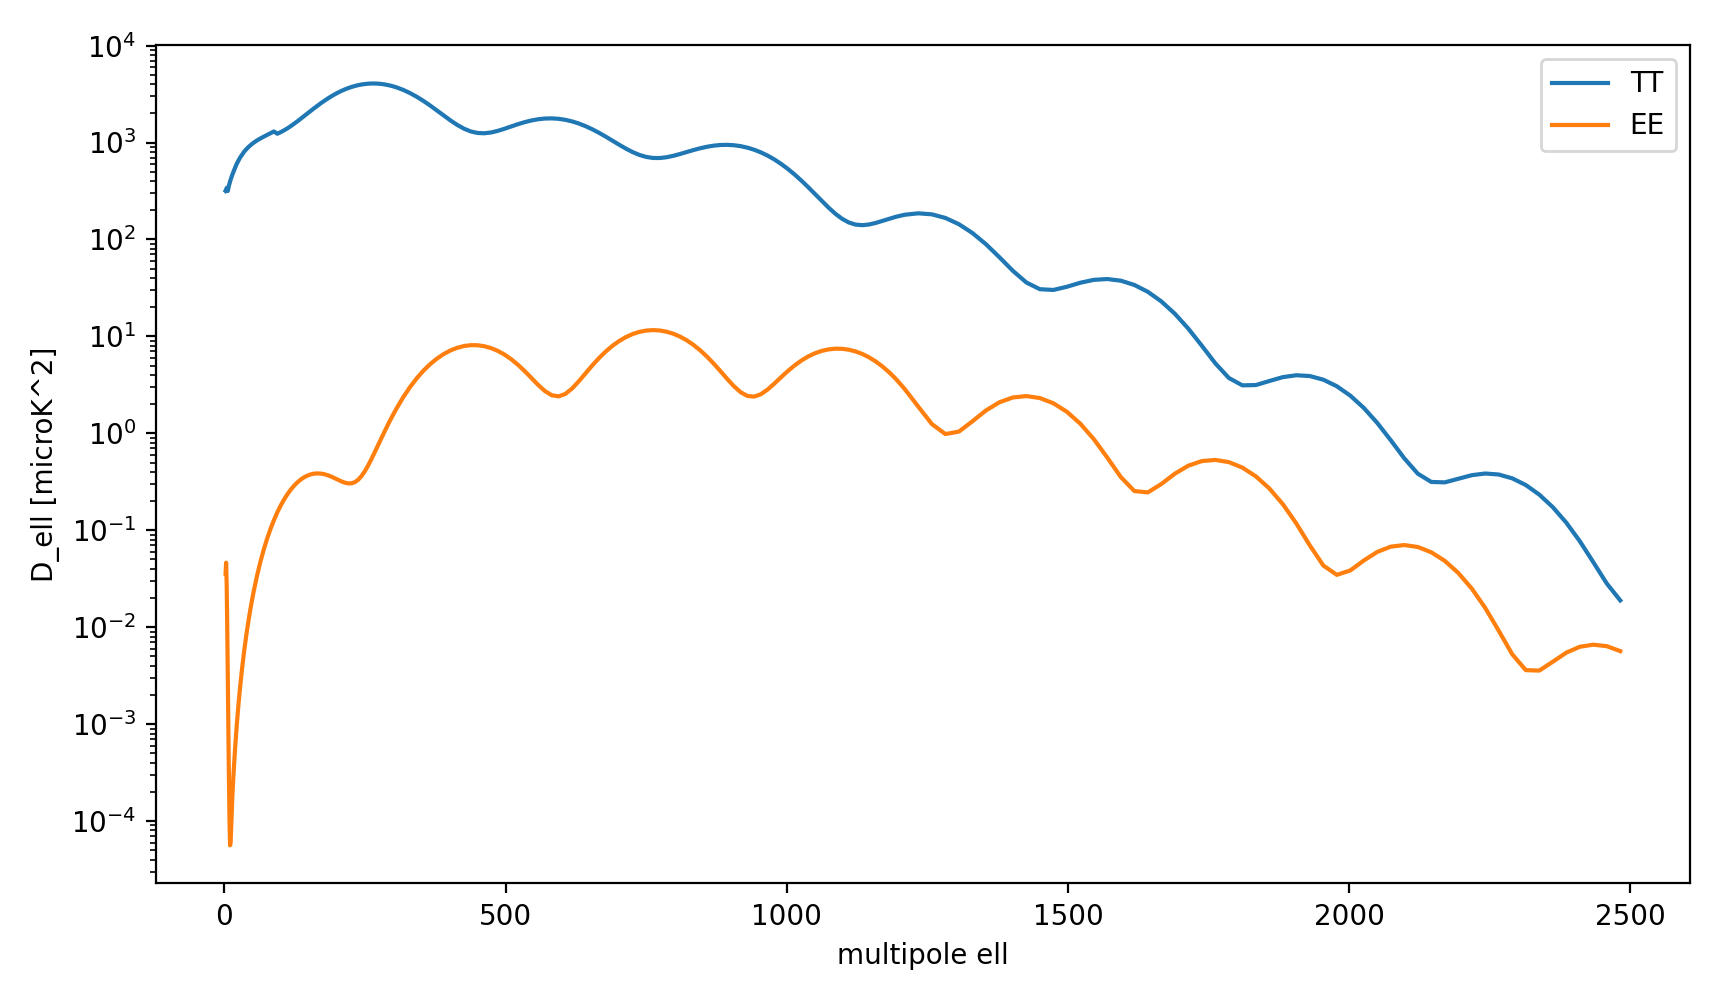
\includegraphics[width=0.88\linewidth]{figures/los/thermal_reionization_tt_ee.png}
\caption{Controlled temperature and scalar $E$-mode templates after effective recombination and reionization.}
\label{fig:trl-tt-ee}
\end{figure}

\begin{figure}[htbp]
\centering
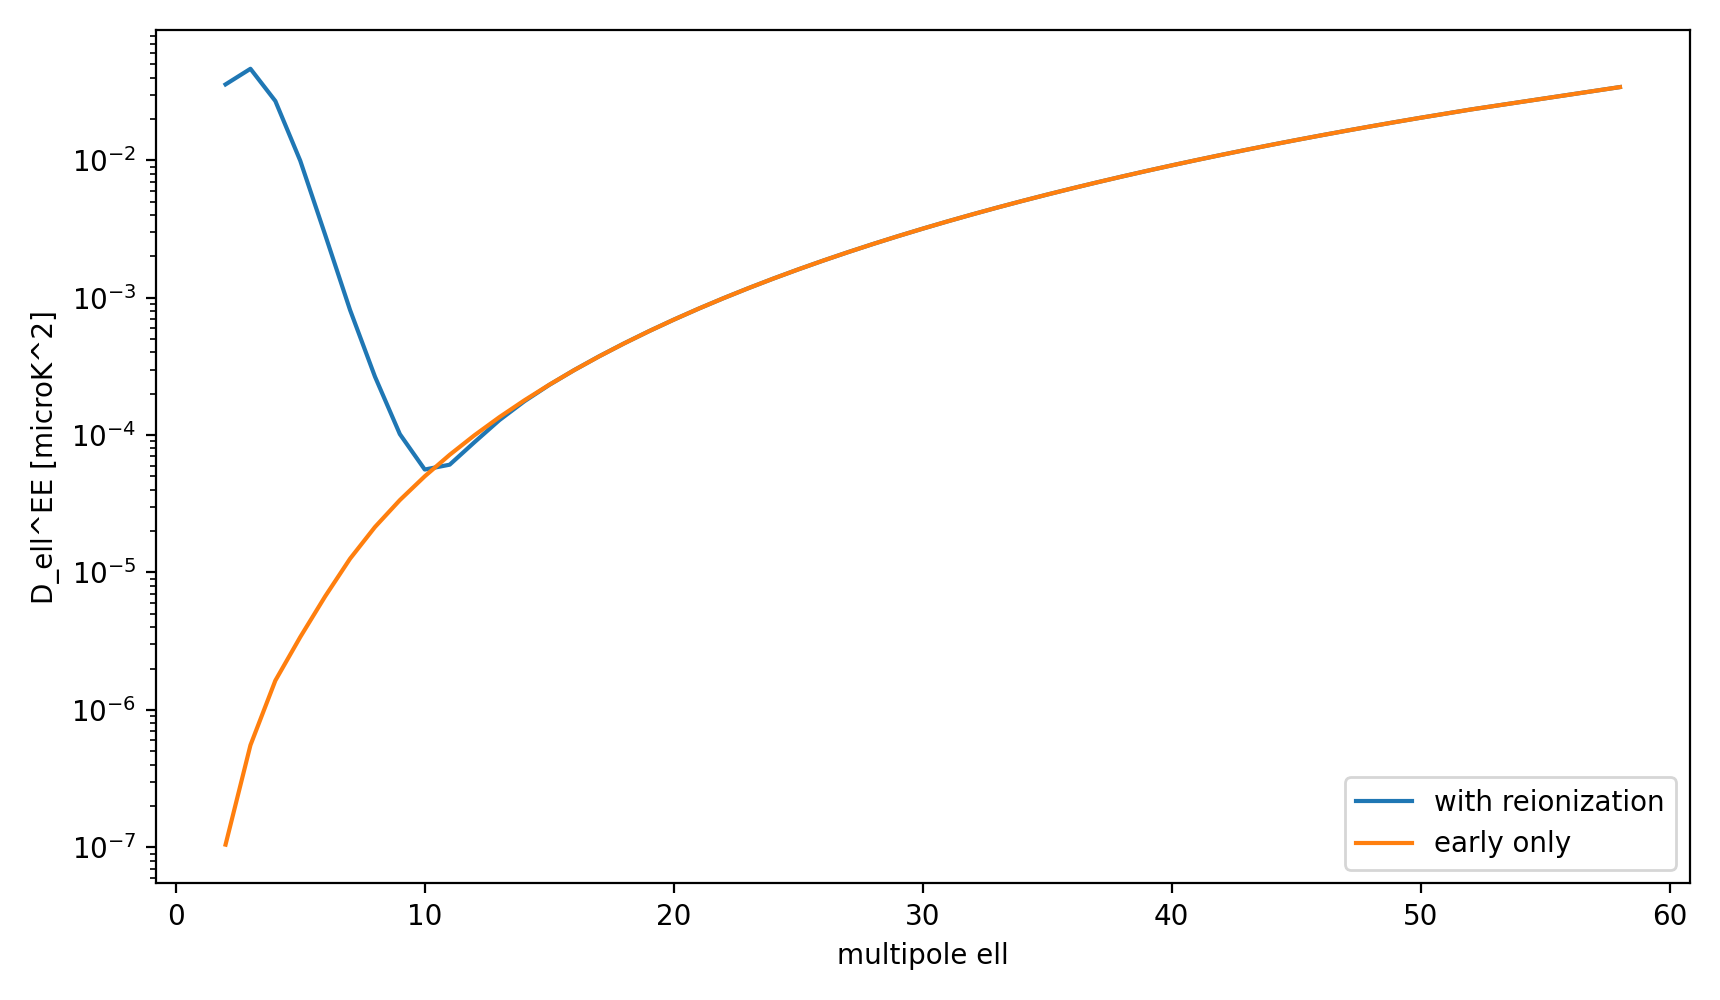
\includegraphics[width=0.84\linewidth]{figures/los/low_ell_ee_bump.png}
\caption{Reionization creates a low-multipole $E$-mode feature absent from the early-only source.}
\label{fig:trl-lowell-ee}
\end{figure}

\begin{figure}[htbp]
\centering
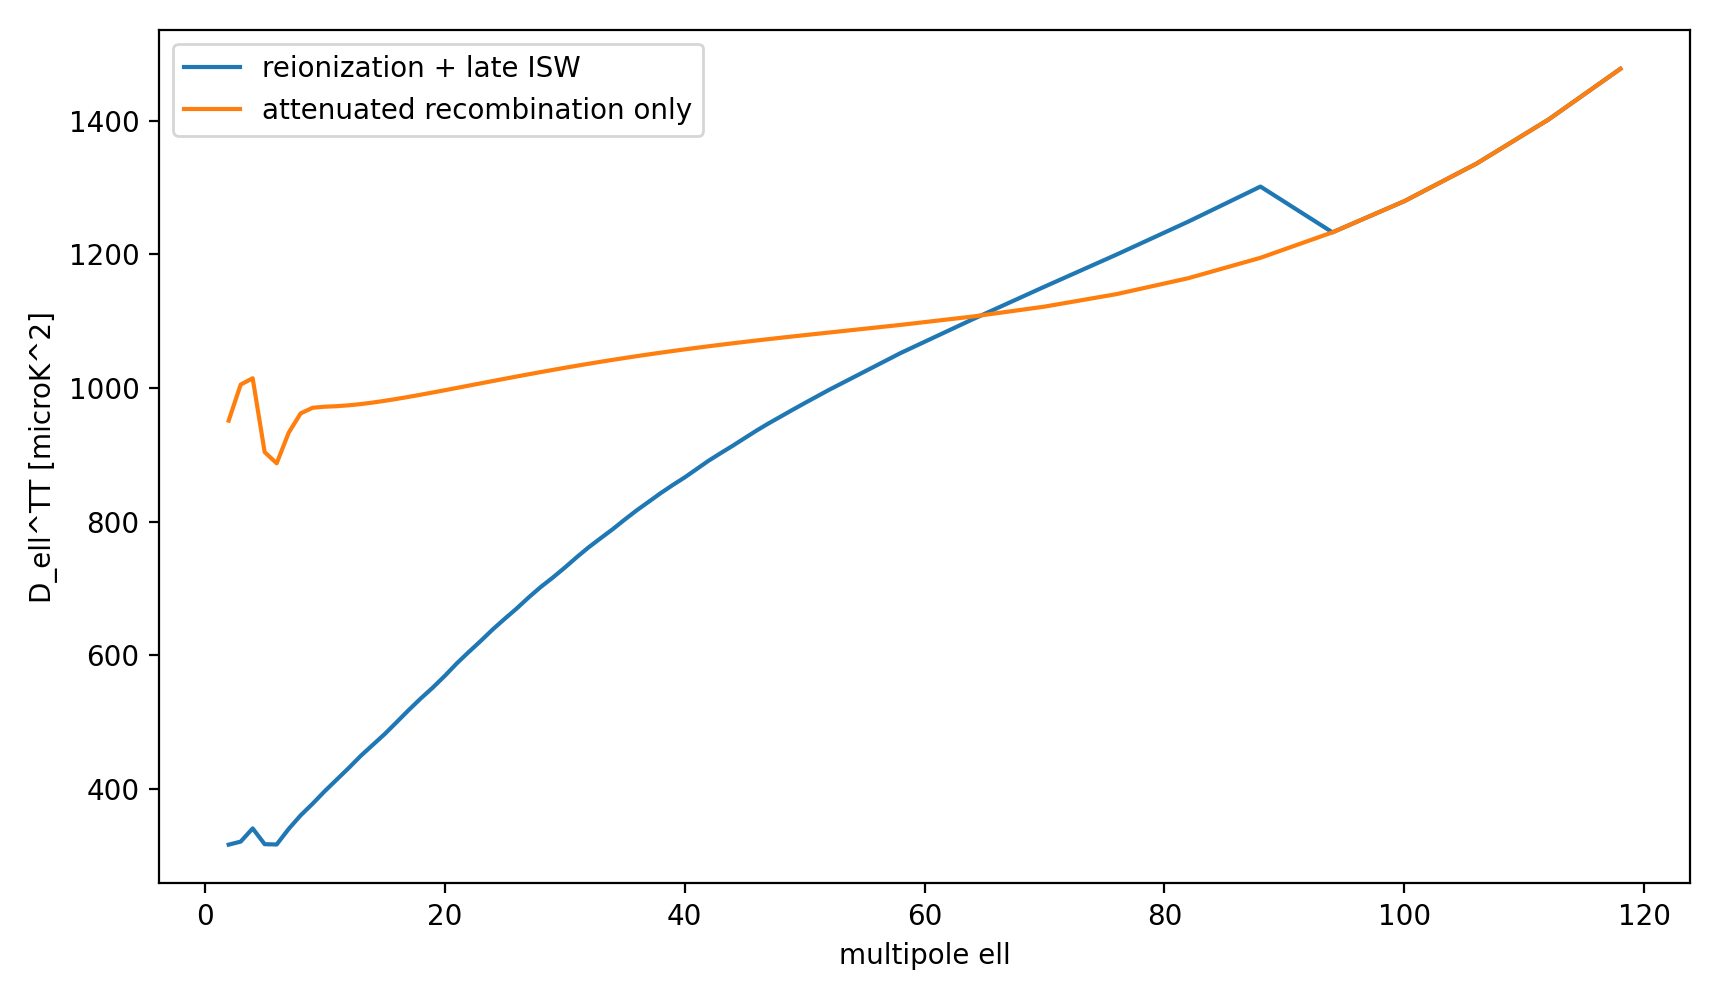
\includegraphics[width=0.84\linewidth]{figures/los/low_ell_tt_late_sources.png}
\caption{Late ISW and reionization modify the low-$\ell$ temperature source while leaving the acoustic regime effectively unchanged in this controlled projection.}
\label{fig:trl-lowell-tt}
\end{figure}

\begin{figure}[htbp]
\centering
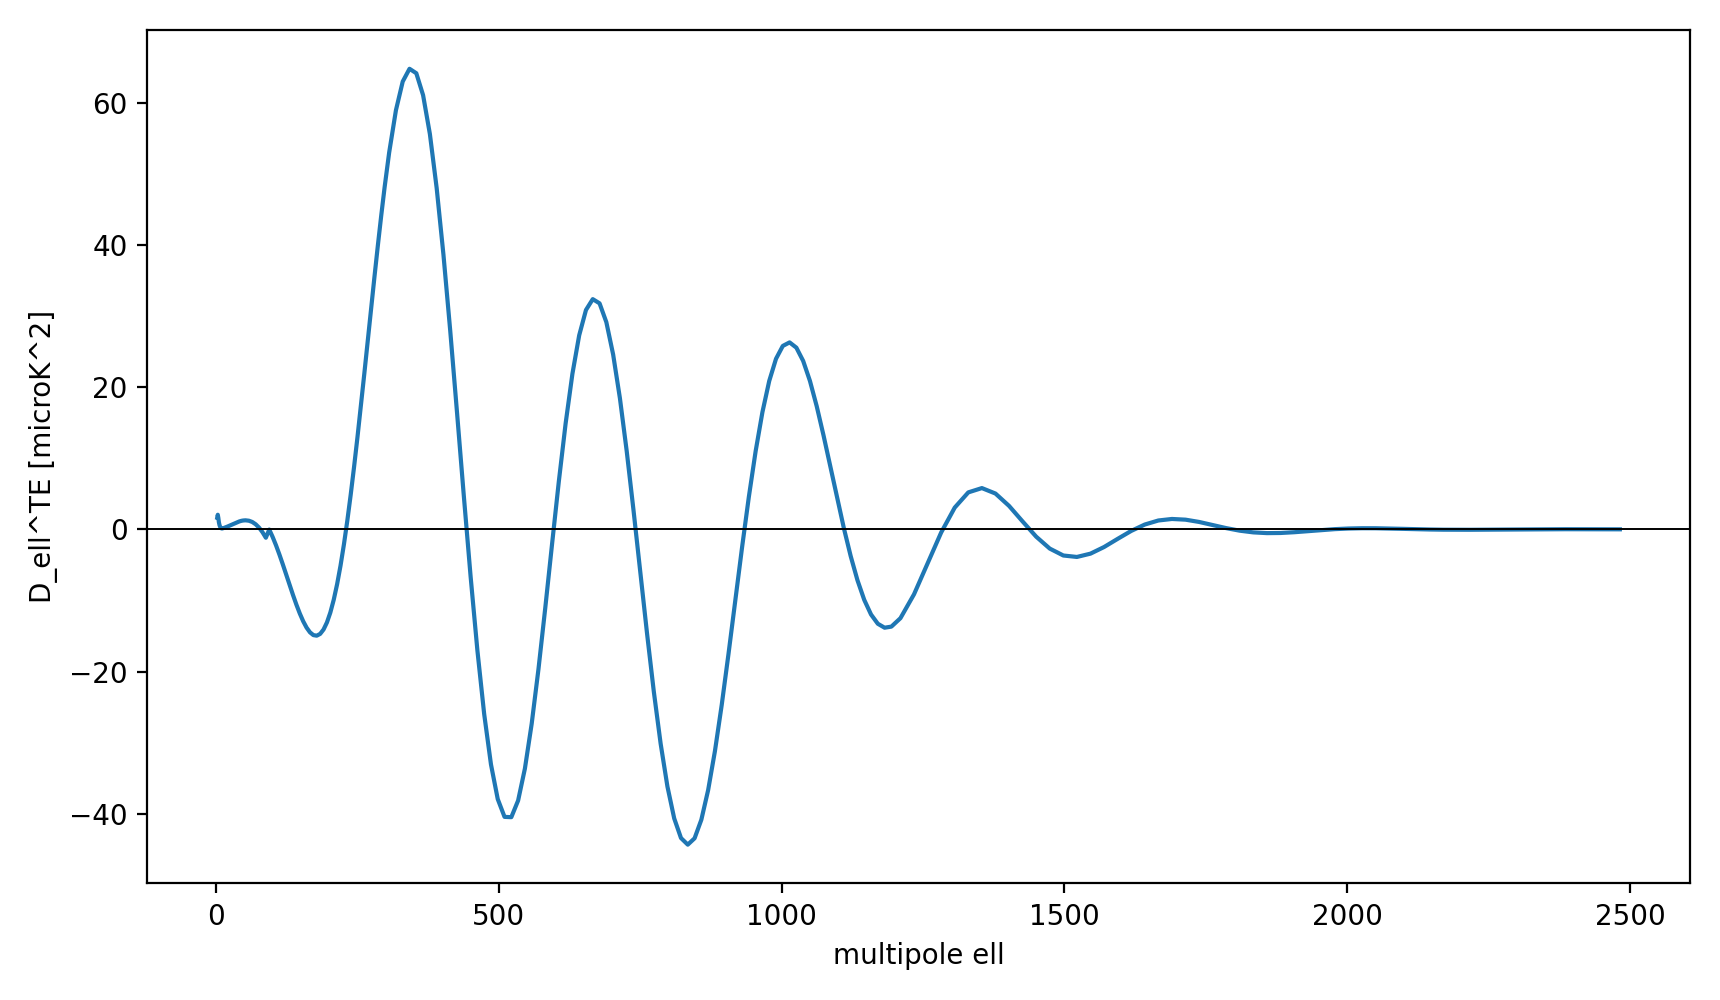
\includegraphics[width=0.88\linewidth]{figures/los/thermal_reionization_te.png}
\caption{Controlled TE template with alternating correlation sign across the acoustic structure.}
\label{fig:trl-te}
\end{figure}

\section{Projection convergence and deterministic audit}

The main projection uses 3350 global wavenumber nodes after combining logarithmic low-$k$ sampling with a linear oscillatory grid.  A 4500-node reference calculation was performed at selected multipoles.

\begin{table}[htbp]
\centering
\begin{tabular}{lrr}
\toprule
control & measured maximum & acceptance bound\\
\midrule
TT selected-grid discrepancy & $1.20461\times10^{-2}$ & $6\times10^{-2}$\\
EE selected-grid discrepancy & $4.42685\times10^{-2}$ & $6\times10^{-2}$\\
TE correlation discrepancy & $7.86181\times10^{-3}$ & $6\times10^{-2}$\\
acoustic TT discrepancy & $1.45217\times10^{-5}$ & $5\times10^{-2}$\\
\bottomrule
\end{tabular}
\caption{Main-to-fine projection convergence.}
\label{tab:trl-convergence}
\end{table}

\begin{figure}[htbp]
\centering
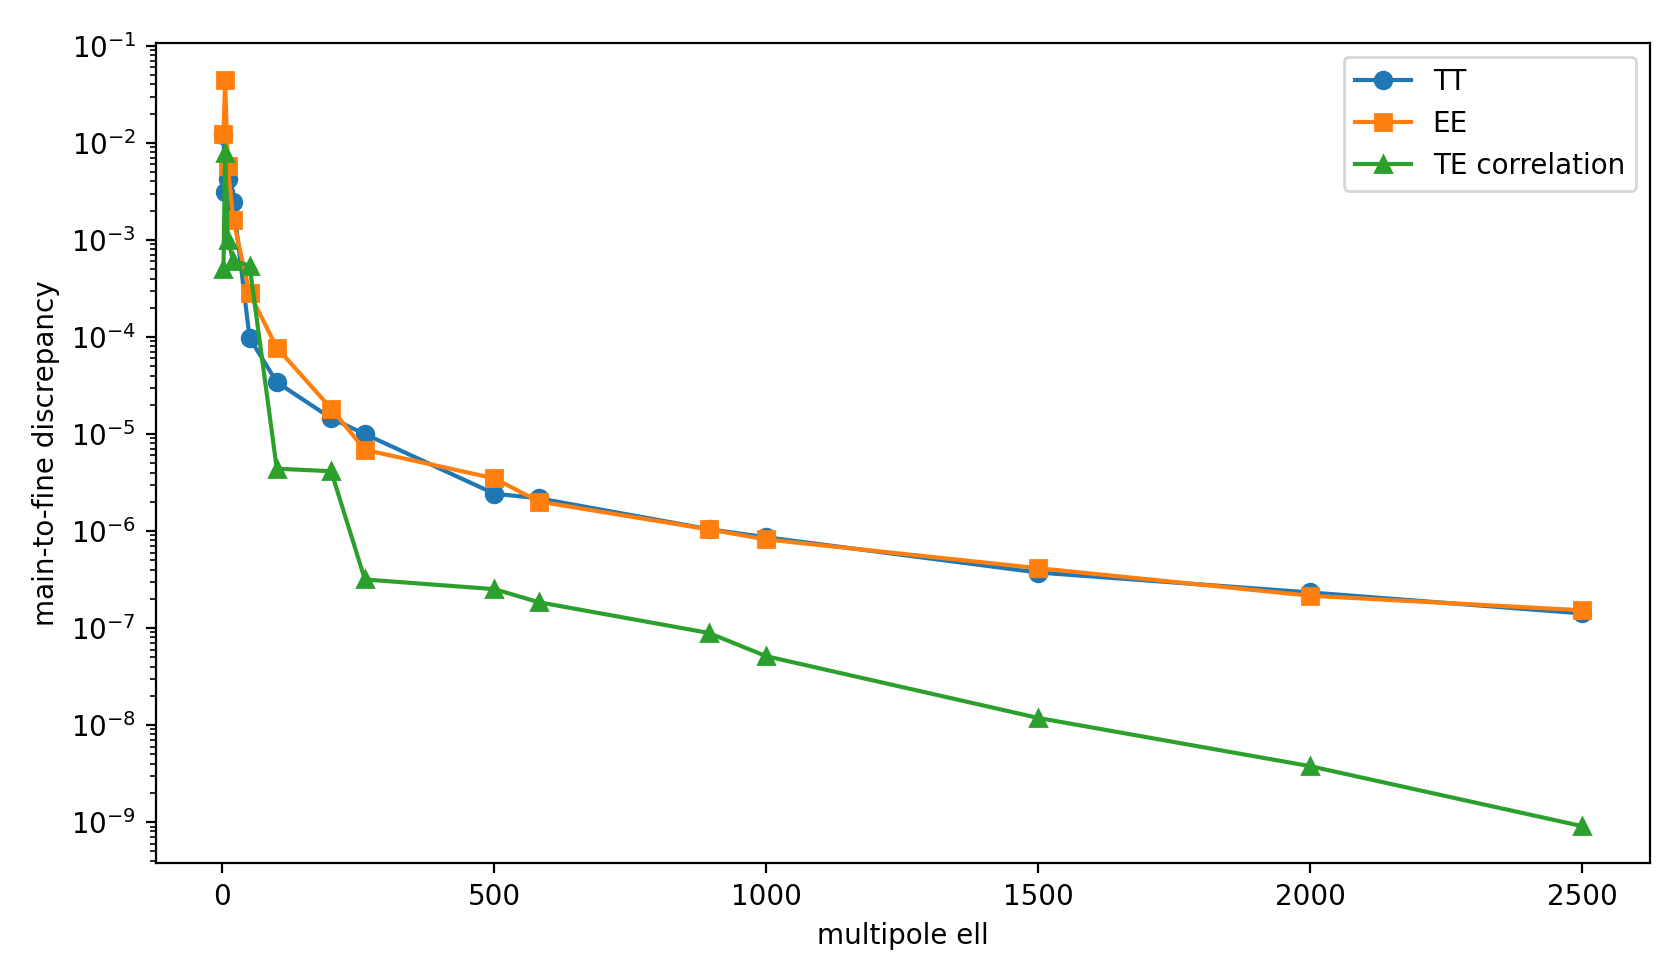
\includegraphics[width=0.82\linewidth]{figures/los/projection_convergence.png}
\caption{Selected-multipole convergence under global wavenumber-grid refinement.}
\label{fig:trl-convergence}
\end{figure}

The main deterministic suite records
\begin{equation}
\boxed{20\ {\rm PASS},\qquad0\ {\rm FAIL},}
\label{eq:trl-main-audit}
\end{equation}
and the independent projection-refinement suite records
\begin{equation}
\boxed{4\ {\rm PASS},\qquad0\ {\rm FAIL}.}
\label{eq:trl-convergence-audit}
\end{equation}
The combined result is
\begin{equation}
\boxed{24\ {\rm PASS},\qquad0\ {\rm FAIL}.}
\label{eq:trl-total-audit}
\end{equation}

\section{Closure ledger}

\begin{center}
\small
\begin{tabular}{p{0.43\linewidth}p{0.21\linewidth}p{0.28\linewidth}}
\toprule
statement & status & boundary\\
\midrule
effective Peebles hydrogen history & closed controlled & three-level approximation\\
controlled helium electron counting & closed conditional & smooth transition model\\
reionization optical depth & calibrated & $\tau_{\rm re}$ remains an input\\
recombination and reionization visibility & closed controlled & declared background\\
single-clock production matching & proved at leading order & no independent modulation\\
independent modulation response & derived & linear response\\
late ISW source sign & corrected & stated Newtonian-gauge convention\\
late time-resolved ISW projection & closed controlled & linear potential growth\\
finite-width recombination projection & closed controlled & central-shell approximation\\
low-$\ell$ reionization polarization & demonstrated & effective source reconstruction\\
precision multilevel H/He recombination & open & atomic kinetics\\
reionization redshift from astrophysics & open & source population\\
full recombination-time LOS integral & open & shell approximation retained\\
CMB lensing remapping & open & nonlinear structure\\
joint likelihood and posterior & open & data interface\\
\bottomrule
\end{tabular}
\end{center}

\section{Synthesis and scope}

This chapter closes three previously separate gaps:
\begin{equation}
\boxed{
\begin{gathered}
\text{production-surface adiabatic matching},\\
\text{effective recombination plus reionization},\\
\text{corrected late line-of-sight temperature and polarization sources}.
\end{gathered}}
\label{eq:trl-closed-chain}
\end{equation}
It also separates a robust statement from a model input.  A single-clock production event is adiabatic at leading gradient order, while an independent modulation field generates a calculable level-dependent entropy response.  The reionization optical depth is calibrated rather than predicted.

\chapter{CMB Lensing Remapping, Lensing \texorpdfstring{$B$}{B} Modes, and Cross-Observable Scale Separation}
\label{ch:cmb-lensing-remapping}

\section{Scope and objective}

The production-to-CMB calculation supplies controlled unlensed $TT$, $TE$, and $EE$ templates, while the collisionless refinement calculation supplies a late-time scale-dependent matter transfer.  The missing linear-observable link was the gravitational remapping between them.  This chapter constructs a common lensing potential, remaps the temperature and polarization fields without retuning the dark sector, generates the scalar lensing $B$ mode, and compares the resulting CMB response with the previously computed galaxy-lensing response.

The result is a controlled Born, flat-sky, Gaussian-remapping benchmark.  It is not a precision CMB-lensing likelihood.  The matter spectrum is normalized to a declared $\sigma_8$ benchmark, its smooth baseline transfer omits baryon wiggles, and nonlinear matter power, post-Born corrections, foregrounds, and delensing are not included.

\section{Matter spectrum and fixed refinement transfer}

Let
\begin{equation}
 \Omega_{m0}=\Omega_{b0}+\Omega_{D0}=0.310,
 \qquad
 \Omega_{r0}=9.0\times10^{-5},
 \qquad
 \Omega_{V0}=1-\Omega_{m0}-\Omega_{r0}.
 \label{eq:lens-background-fractions}
\end{equation}
The background is
\begin{equation}
 E(a)^2=\Omega_{r0}a^{-4}+\Omega_{m0}a^{-3}+\Omega_{V0}.
 \label{eq:lens-background}
\end{equation}
A smooth control matter spectrum is written
\begin{equation}
 P_{\rm c}(k,0)=A_P k^{n_s}T_{\rm sm}(k)^2,
 \label{eq:lens-control-power}
\end{equation}
where the amplitude $A_P$ is fixed by
\begin{equation}
 \sigma_8^2
 =\int_0^\infty \frac{k^3P_{\rm c}(k,0)}{2\pi^2}
 W_{\rm TH}(kR_8)^2\,d\log k,
 \qquad
 R_8=\frac{8}{h}\ {\rm Mpc}.
 \label{eq:lens-sigma8-normalization}
\end{equation}
The deterministic calculation uses
\begin{equation}
 n_s=0.965,
 \qquad
 \sigma_8=0.81.
 \label{eq:lens-normalization-values}
\end{equation}
The refinement matter spectrum is not refitted.  It is
\begin{equation}
 P_D(k,a)=D(a)^2T_D(k)^2P_{\rm c}(k,0),
 \label{eq:lens-refinement-power}
\end{equation}
where $T_D(k)$ is the momentum-resolved collisionless transfer already derived from the scale-covariant production distribution.

\section{CMB convergence and lensing potential}

For a source plane at comoving distance $\chi_*$, define
\begin{equation}
 W_\kappa(\chi)
 =\frac{3}{2}\Omega_{m0}\left(\frac{H_0}{c}\right)^2
 \frac{\chi}{a(\chi)}\frac{\chi_*-\chi}{\chi_*}.
 \label{eq:lens-kernel}
\end{equation}
The Limber convergence spectrum is
\begin{equation}
 C_L^{\kappa\kappa}
 =\int_0^{\chi_*}\frac{d\chi}{\chi^2}
 W_\kappa(\chi)^2
 P_m\!\left(\frac{L+1/2}{\chi},a(\chi)\right).
 \label{eq:lens-kappa-spectrum}
\end{equation}
The lensing-potential spectrum is
\begin{equation}
 C_L^{\phi\phi}
 =\frac{4C_L^{\kappa\kappa}}{L^2(L+1)^2}.
 \label{eq:lens-phi-spectrum}
\end{equation}
The source distance inherited from the effective recombination calculation is
\begin{equation}
 \chi_*=13420.1231642\ {\rm Mpc}.
 \label{eq:lens-source-distance}
\end{equation}

\subsection{Positive-kernel monotonicity}

Assume
\begin{equation}
 0\leq T_D(k)\leq1.
 \label{eq:lens-transfer-order}
\end{equation}
Then the Limber kernel in \eqref{eq:lens-kappa-spectrum} is nonnegative, and therefore
\begin{equation}
 \boxed{
 C_{L,D}^{\kappa\kappa}
 \leq
 C_{L,{\rm c}}^{\kappa\kappa}
 }
 \label{eq:lens-monotonicity}
\end{equation}
for every retained $L$.  Hence
\begin{equation}
 C_{L,D}^{\phi\phi}\leq C_{L,{\rm c}}^{\phi\phi},
 \qquad
 \langle |\boldsymbol\alpha_D|^2\rangle
 \leq
 \langle |\boldsymbol\alpha_{\rm c}|^2\rangle.
 \label{eq:lens-deflection-order}
\end{equation}
This connects the small-scale matter cutoff to a definite sign in every linear lensing-power observable.

\begin{figure}[htbp]
\centering
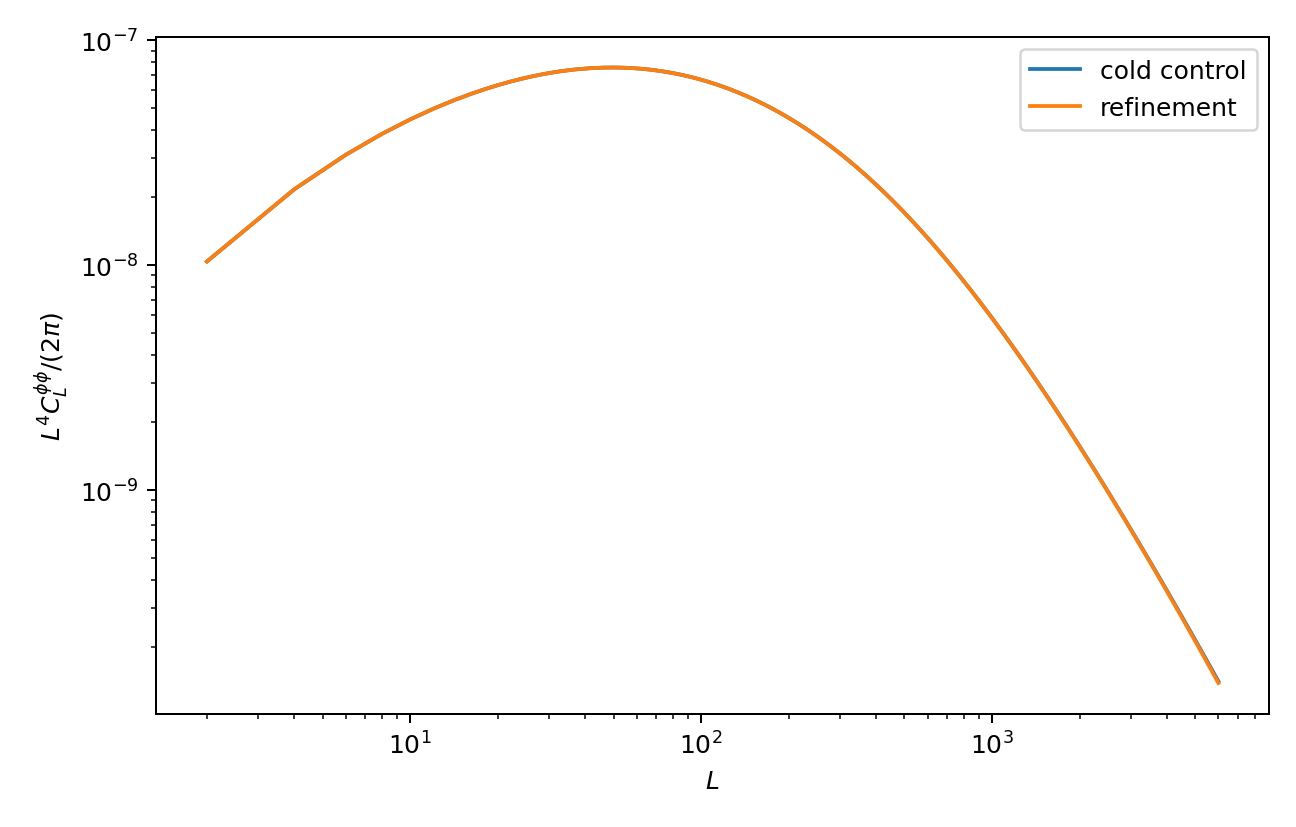
\includegraphics[width=0.86\textwidth]{figures/lens/cmb_lensing_potential.png}
\caption{The controlled CMB lensing-potential spectra.  The refinement and cold-control curves nearly coincide over the dominant CMB-lensing range because the refinement cutoff lies at substantially higher physical wavenumber.}
\label{fig:cmb-lensing-potential}
\end{figure}

\begin{figure}[htbp]
\centering
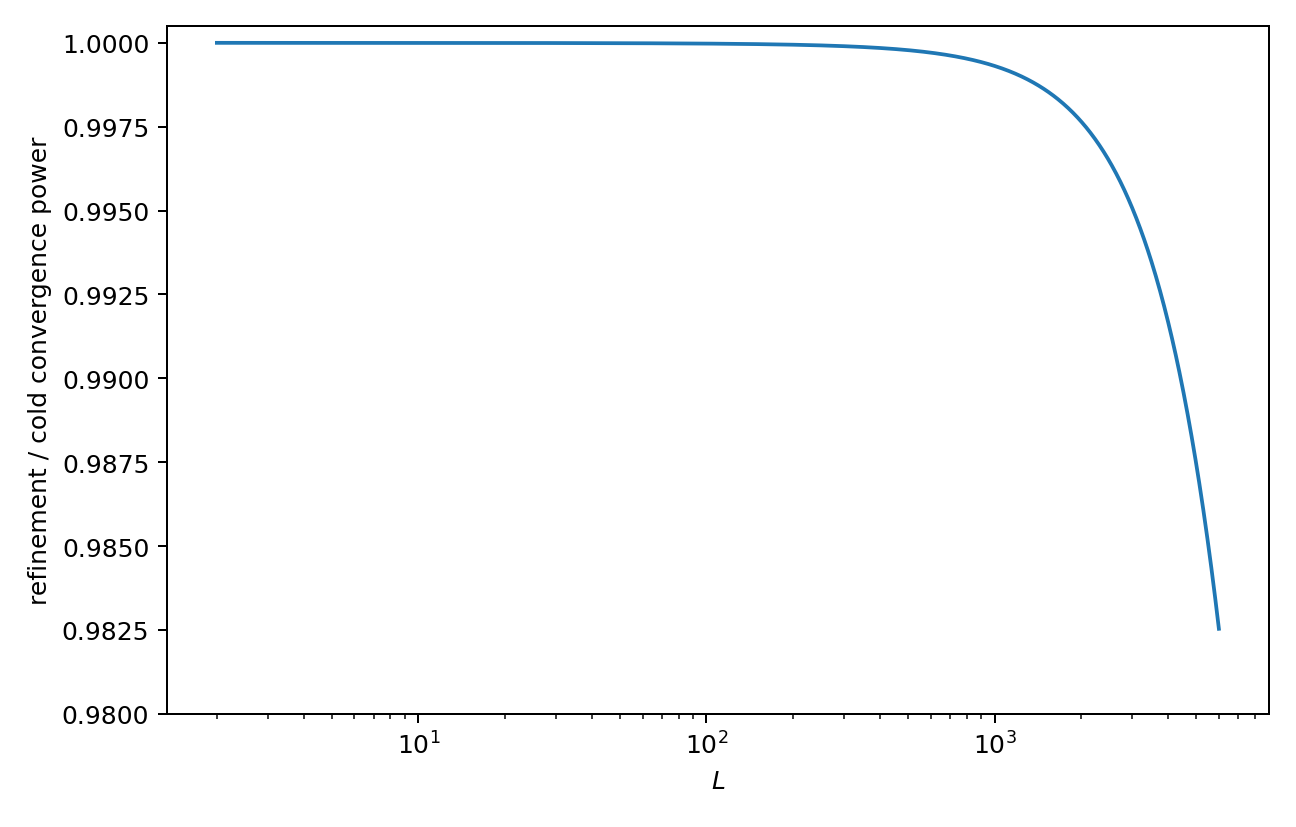
\includegraphics[width=0.82\textwidth]{figures/lens/cmb_lensing_ratio.png}
\caption{Refinement-to-cold convergence-power ratio.  The suppression grows toward high $L$, as required by the positive-kernel theorem.}
\label{fig:cmb-lensing-ratio}
\end{figure}

\section{Deflection variance and finite-patch realization}

In the continuum flat-sky normalization,
\begin{equation}
 \langle |\boldsymbol\alpha|^2\rangle
 =\int_0^\infty\frac{L^3C_L^{\phi\phi}}{2\pi}\,dL.
 \label{eq:lens-alpha-continuum}
\end{equation}
The resulting continuum rms deflections are
\begin{equation}
 \alpha_{\rm rms,c}=1.7890468022\ {\mathrm{arcmin}},
 \qquad
 \alpha_{\rm rms,D}=1.7889974544\ {\mathrm{arcmin}}.
 \label{eq:lens-alpha-values}
\end{equation}

For a periodic square of area $A$, the discrete Fourier expectation is
\begin{equation}
 \boxed{
 \langle |\boldsymbol\alpha|^2\rangle_A
 =\frac{1}{A}\sum_{\boldsymbol L}
 L^2C_L^{\phi\phi}.
 }
 \label{eq:lens-alpha-box}
\end{equation}
The principal realization uses a $20^\circ$ square, $512^2$ pixels, and forty-eight paired Gaussian realizations.  The finite box excludes the lowest deflection modes and gives
\begin{equation}
 \alpha_{\rm rms,c}^{\rm box}=1.6259829378\ {\mathrm{arcmin}},
 \qquad
 \alpha_{\rm rms,D}^{\rm box}=1.6259306696\ {\mathrm{arcmin}}.
 \label{eq:lens-alpha-box-values}
\end{equation}
The measured and discrete-expectation variances agree to $5.7\times10^{-4}$ relative accuracy.

\section{Nonperturbative map remapping}

Let $X\in\{T,Q,U\}$.  The Born remapping is
\begin{equation}
 \widetilde X(\boldsymbol n)
 =X\!\left(\boldsymbol n+\nabla\phi(\boldsymbol n)\right).
 \label{eq:lens-remap}
\end{equation}
On the flat sky,
\begin{equation}
 Q(\boldsymbol\ell)
 =E(\boldsymbol\ell)\cos2\varphi_\ell
 -B(\boldsymbol\ell)\sin2\varphi_\ell,
 \label{eq:lens-q-eb}
\end{equation}
\begin{equation}
 U(\boldsymbol\ell)
 =E(\boldsymbol\ell)\sin2\varphi_\ell
 +B(\boldsymbol\ell)\cos2\varphi_\ell.
 \label{eq:lens-u-eb}
\end{equation}
The unlensed scalar template has
\begin{equation}
 B(\boldsymbol\ell)=0.
 \label{eq:lens-unlensed-b-zero}
\end{equation}
After remapping, the inverse spin rotation produces
\begin{equation}
 \widetilde B(\boldsymbol\ell)
 =-\widetilde Q(\boldsymbol\ell)\sin2\varphi_\ell
 +\widetilde U(\boldsymbol\ell)\cos2\varphi_\ell,
 \label{eq:lens-generated-b}
\end{equation}
which is nonzero even though the primordial scalar $B$ mode vanishes.

The same primary Gaussian realization and the same lensing phases are used for the cold and refinement runs.  This paired design isolates the small difference generated by $T_D(k)$ from Monte Carlo variance.

\section{Remapped temperature and polarization}

The remapping smooths the acoustic pattern.  Around the second temperature peak, the declared peak-to-neighboring-trough contrast changes from
\begin{equation}
 \mathcal C_2^{\rm unlensed}=0.4493968827
 \label{eq:lens-contrast-unlensed}
\end{equation}
to
\begin{equation}
 \mathcal C_2^{\rm lensed}=0.4382775755.
 \label{eq:lens-contrast-lensed}
\end{equation}
Thus
\begin{equation}
 \boxed{
 \frac{\mathcal C_2^{\rm lensed}}
 {\mathcal C_2^{\rm unlensed}}
 =0.9752572669<1.
 }
 \label{eq:lens-contrast-ratio}
\end{equation}

\begin{figure}[htbp]
\centering
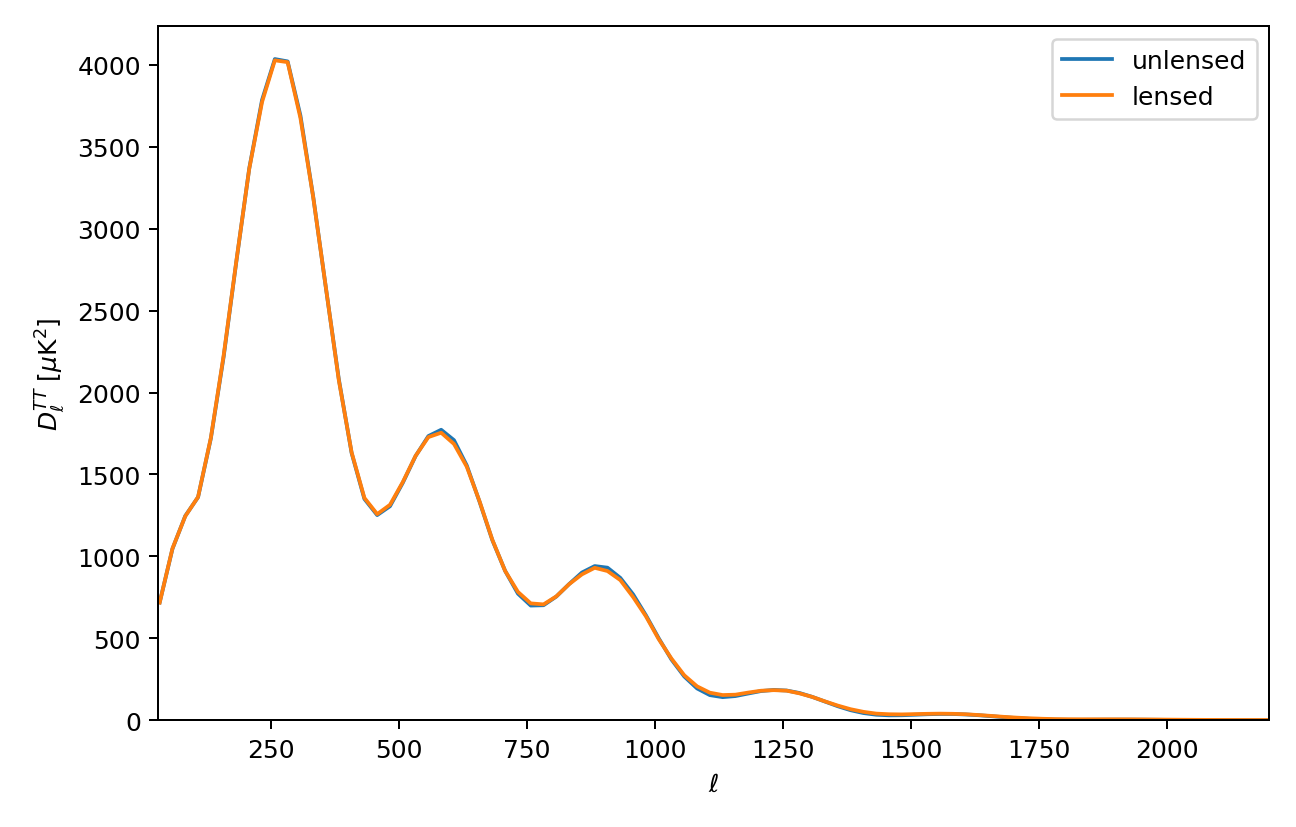
\includegraphics[width=0.88\textwidth]{figures/lens/lensed_temperature_spectrum.png}
\caption{Unlensed and lensed controlled temperature templates.  The remapping reduces acoustic contrast and transfers power into the damped high-$\ell$ tail.}
\label{fig:lensed-temperature}
\end{figure}

Selected remapped values are
\begin{center}
\begin{tabular}{rrrrr}
\toprule
$\ell$ & $D_\ell^{TT,{\rm unl}}$ & $D_\ell^{TT,{\rm len}}$ & $D_\ell^{EE,{\rm len}}$ & $D_\ell^{BB,{\rm len}}$\\
& $[\mu{\rm K}^2]$ & $[\mu{\rm K}^2]$ & $[\mu{\rm K}^2]$ & $[\mu{\rm K}^2]$\\
\midrule
$108$  & $1361.5425$ & $1362.8868$ & $0.21436$ & $8.5890\times10^{-4}$\\
$258$  & $4035.0350$ & $4027.3441$ & $0.51018$ & $5.3587\times10^{-3}$\\
$508$  & $1449.1799$ & $1453.8814$ & $5.91811$ & $1.29145\times10^{-2}$\\
$1008$ & $500.9239$  & $495.4583$  & $4.69624$ & $1.42386\times10^{-2}$\\
$1508$ & $33.8350$   & $37.7772$   & $1.46534$ & $7.5177\times10^{-3}$\\
$2008$ & $2.31049$   & $3.99422$   & $0.06954$ & $4.1477\times10^{-3}$\\
\bottomrule
\end{tabular}
\end{center}

\section{Scalar lensing \texorpdfstring{$B$}{B} mode}

The generated lensing $B$ template peaks near the acoustic-to-damping transition.  In the principal realization,
\begin{equation}
 \boxed{
 D_{1008}^{BB,{\rm lens}}
 =1.4238587\times10^{-2}\ \mu{\rm K}^2,
 }
 \label{eq:lens-bb-1000}
\end{equation}
\begin{equation}
 \boxed{
 D_{2008}^{BB,{\rm lens}}
 =4.1477498\times10^{-3}\ \mu{\rm K}^2.
 }
 \label{eq:lens-bb-2000}
\end{equation}
The refinement-to-cold ratios are
\begin{equation}
 \frac{D_{1008,D}^{BB}}{D_{1008,{\rm c}}^{BB}}
 =0.9997167797,
 \qquad
 \frac{D_{2008,D}^{BB}}{D_{2008,{\rm c}}^{BB}}
 =0.9990054398.
 \label{eq:lens-bb-ratios}
\end{equation}
Thus the benchmark predicts an ordinary-looking scalar lensing $B$ mode over the main CMB range, despite the much stronger cutoff in sufficiently small-scale low-redshift structure.

\begin{figure}[htbp]
\centering
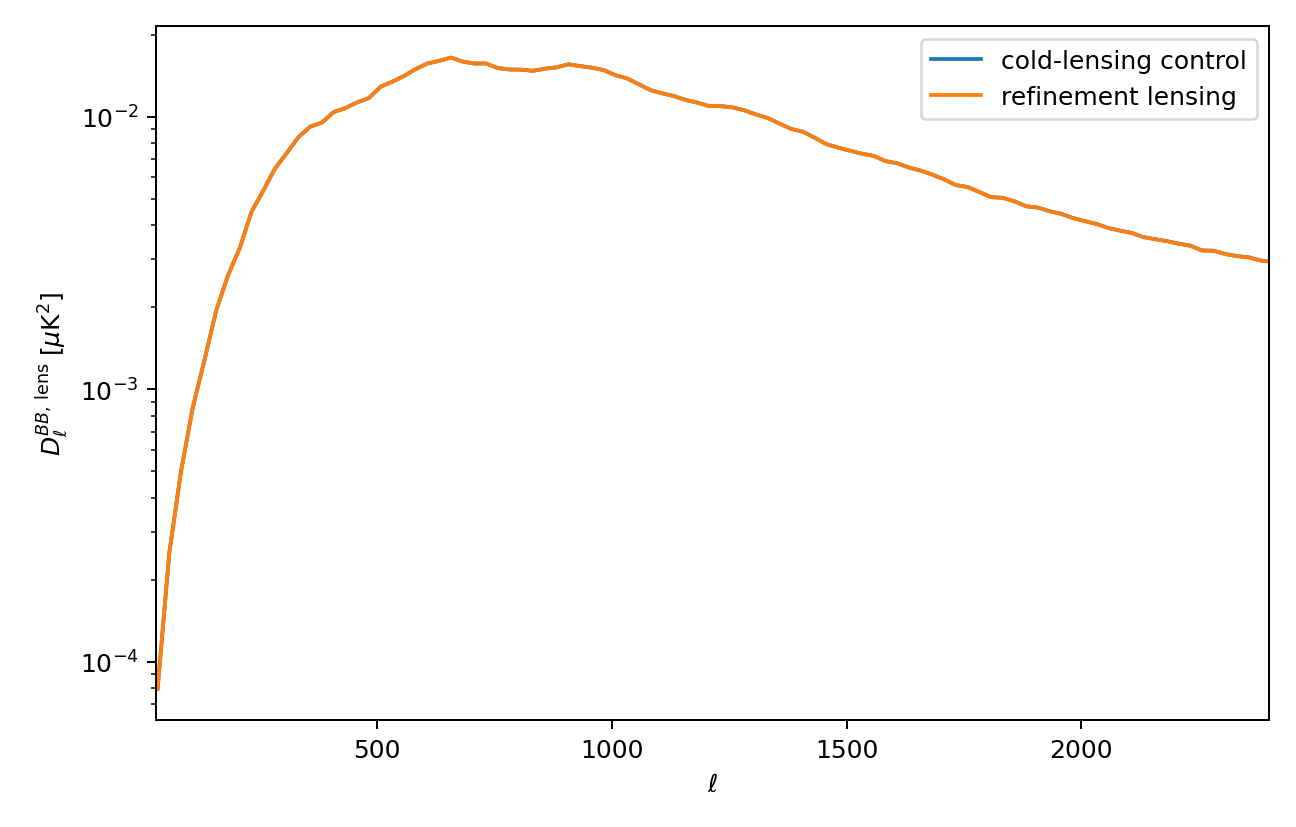
\includegraphics[width=0.86\textwidth]{figures/lens/lensing_b_modes.png}
\caption{Lensing-generated scalar $B$-mode templates.  The two curves are nearly coincident because the CMB lensing kernel mainly samples wavenumbers below the refinement half-mode scale.}
\label{fig:lensing-bmodes}
\end{figure}

\section{Cross-observable scale separation}

The CMB convergence-power ratios are
\begin{equation}
 \frac{C_{1000,D}^{\kappa\kappa}}
 {C_{1000,{\rm c}}^{\kappa\kappa}}
 =0.9993089943,
 \label{eq:lens-kappa-ratio-1000}
\end{equation}
\begin{equation}
 \frac{C_{3000,D}^{\kappa\kappa}}
 {C_{3000,{\rm c}}^{\kappa\kappa}}
 =0.9950809554,
 \qquad
 \frac{C_{5000,D}^{\kappa\kappa}}
 {C_{5000,{\rm c}}^{\kappa\kappa}}
 =0.9874740972.
 \label{eq:lens-kappa-ratio-high}
\end{equation}
The prior linear galaxy-lensing calculation gives, for a source at $z_s=0.5$,
\begin{equation}
 \frac{C_{5000,D}^{\kappa\kappa}(z_s=0.5)}
 {C_{5000,{\rm c}}^{\kappa\kappa}(z_s=0.5)}
 =0.7021280719.
 \label{eq:lens-galaxy-ratio}
\end{equation}
The same microscopic transfer therefore produces a scale- and kernel-dependent hierarchy:
\begin{equation}
 \boxed{
 \text{primary CMB lensing: nearly cold}
 \quad\text{while}\quad
 \text{low-redshift high-}\ell\text{ lensing: strongly suppressed}.
 }
 \label{eq:lens-scale-separation}
\end{equation}
The reason is geometric.  At fixed angular multipole, a lower-distance kernel probes larger physical wavenumber $k\simeq(L+1/2)/\chi$, and therefore reaches the refinement cutoff earlier.

\begin{figure}[htbp]
\centering
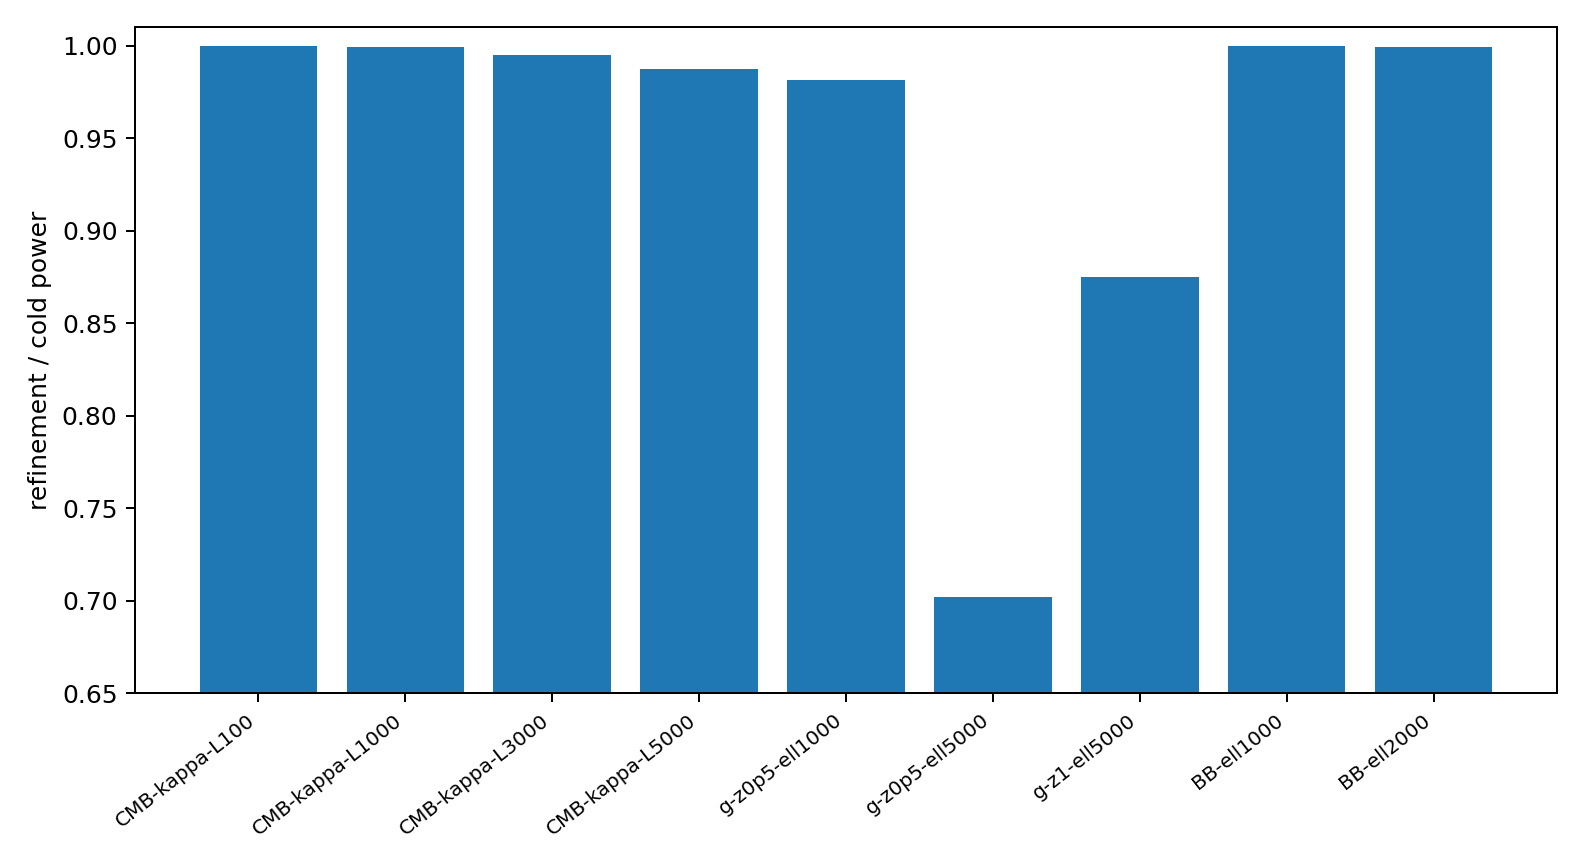
\includegraphics[width=0.94\textwidth]{figures/lens/cross_observable_scale_separation.png}
\caption{Linked lensing observables generated from the same refinement transfer.  The strong low-redshift suppression coexists with percent-level or smaller CMB-lensing corrections.}
\label{fig:lens-cross-observable}
\end{figure}

\section{Verification and convergence}

The deterministic audit records
\begin{equation}
 \boxed{
 20\ {\rm PASS},
 \qquad
 0\ {\rm FAIL}.
 }
 \label{eq:lens-pass-count}
\end{equation}
The principal controls are
\begin{center}
\begin{tabular}{lr}
\toprule
control & residual or discrepancy\\
\midrule
$\sigma_8$ reconstruction & $1.11\times10^{-16}$\\
finite-box cold deflection variance & $5.62\times10^{-4}$\\
finite-box refinement deflection variance & $5.62\times10^{-4}$\\
24-to-48 realization refinement & $1.694\times10^{-2}$\\
$448^2$-to-$512^2$ grid refinement & $1.034\times10^{-1}$\\
maximum lensed $TE$ Cauchy ratio & $0.640576<1$\\
\bottomrule
\end{tabular}
\end{center}
The grid discrepancy is dominated by the lensing $B$ tail near $\ell\simeq2000$.  Temperature and $E$-mode discrepancies are substantially smaller.  The output beyond the parent acoustic range is retained as a controlled extrapolative tail rather than a precision prediction.

\section{Closure ledger}

\begin{center}
\begin{tabularx}{\textwidth}{>{\raggedright\arraybackslash}X>{\raggedright\arraybackslash}p{0.18\textwidth}>{\raggedright\arraybackslash}p{0.24\textwidth}}
\toprule
statement & status & boundary\\
\midrule
CMB convergence and lensing potential from the fixed refinement transfer & closed controlled & linear Limber and declared $\sigma_8$ normalization\\
positive-kernel suppression theorem & proved & $0\leq T_D\leq1$\\
finite-patch Gaussian deflection realization & closed controlled & periodic flat sky\\
nonperturbative Born remapping of $T,Q,U$ & closed controlled & no post-Born correction\\
scalar lensing $B$-mode template & closed controlled & no primordial tensor $B$ mode\\
linked CMB and galaxy lensing hierarchy & closed conditional & linear source kernels\\
nonlinear matter lensing & open & nonlinear power and baryonic feedback\\
precision full-sky remapping and covariance & open & production analysis code\\
observational likelihood and parameter posterior & open & data, nuisance, and covariance model\\
\bottomrule
\end{tabularx}
\end{center}

\section{Synthesis and unresolved requirements}

The scale-covariant dark sector now predicts, with one unchanged transfer function,
\begin{equation}
 \boxed{
 \begin{gathered}
 \text{matter cutoff}
 \Longrightarrow
 \text{galaxy-lensing suppression}
 \Longrightarrow
 \text{CMB lensing potential}\\
 \Longrightarrow
 \text{remapped }TT,TE,EE
 \Longrightarrow
 \text{lensing }BB
 \end{gathered}
 }
 \label{eq:lens-result-chain}
\end{equation}
The remaining observational requirements are
\begin{equation}
 \boxed{
 \begin{gathered}
 \text{nonlinear matter and halo evolution},\\
 \text{baryonic and astrophysical nuisance sectors},\\
 \text{precision full-sky CMB remapping},\\
 \text{one joint likelihood with frozen microscopic parameters}.
 \end{gathered}
 }
 \label{eq:lens-open-requirements}
\end{equation}

\chapter[Nonlinear Structure and Reionization]{Nonlinear Structure, Halo Formation, and Reionization Consistency}
\PhysicsContext{From linear transport to structure}{The fourth part tests whether the linear cutoff survives nonlinear gravity and astrophysical response. Several initially strong linear signatures are weakened or rendered sign-indefinite by this progression.}


\label{ch:nonlinear-structure-halo}

\section{Scope and objective}

The scale-covariant refinement sector now supplies a linear collisionless transfer, primary-CMB templates, reionization, and CMB lensing.  The remaining major structure-formation question is whether the linear small-scale cutoff survives nonlinear collapse, and whether the same cutoff is compatible with the early halo population needed by the calibrated reionization history.

This chapter performs a controlled nonlinear consistency audit.  It combines the fixed collisionless transfer with a spherical-collapse calculation, an excursion-set halo abundance, a formation-time concentration model, a compensated halo model, nonlinear lensing projection, and an atomic-cooling collapsed-fraction test.  No dark-sector parameter is retuned.

The principal conclusion is mixed and therefore important:
\begin{equation}
 \boxed{
 \begin{gathered}
 \text{low-mass halo abundance and high-redshift collapse remain strongly suppressed},\\
 \text{but nonlinear halo formation regenerates much of the small-scale power}. 
 \end{gathered}}
 \label{eq:nlh-central-result}
\end{equation}
Consequently, the earlier linear high-$\ell$ galaxy-lensing deficit is not a robust final prediction once a controlled nonlinear halo model is inserted.  The cleaner surviving signatures are the low-mass halo mass function, delayed halo formation, reduced concentrations, and the ionizing-efficiency burden at high redshift.

\section{Fixed linear input and variance ordering}

Let the cold-control spectrum be
\begin{equation}
 P_{\rm c}(k,z)=D(z)^2P_{\rm c}(k,0),
 \label{eq:nlh-cold-power}
\end{equation}
and let the refinement spectrum be
\begin{equation}
 P_D(k,z)=T_D(k)^2P_{\rm c}(k,z),
 \qquad
 0\leq T_D(k)\leq1.
 \label{eq:nlh-dark-power}
\end{equation}
The amplitude is normalized by
\begin{equation}
 \sigma_8=0.81.
 \label{eq:nlh-sigma8}
\end{equation}
For a spherical top-hat containing mass $M$,
\begin{equation}
 R(M)=\left(\frac{3M}{4\pi\bar\rho_m}\right)^{1/3},
 \label{eq:nlh-radius}
\end{equation}
and
\begin{equation}
 \sigma_X^2(M,z)
 =\int_0^\infty
 \frac{k^3P_X(k,z)}{2\pi^2}
 W_{\rm TH}(kR)^2\,d\log k,
 \qquad
 X\in\{\mathrm c,D\}.
 \label{eq:nlh-variance}
\end{equation}
Because the kernel is nonnegative,
\begin{equation}
 \boxed{
 \sigma_D^2(M,z)\leq\sigma_{\rm c}^2(M,z)
 }
 \label{eq:nlh-variance-ordering}
\end{equation}
for every mass and redshift in the declared linear model.  Hence the peak height
\begin{equation}
 \nu_X(M,z)=\frac{\delta_c(z)}{\sigma_X(M,z)}
 \label{eq:nlh-peak-height}
\end{equation}
satisfies
\begin{equation}
 \nu_D(M,z)\geq\nu_{\rm c}(M,z).
 \label{eq:nlh-peak-order}
\end{equation}
This establishes delayed collapse before any halo-mass-function prescription is chosen.

The transfer half-mode is defined by
\begin{equation}
 T_D(k_{1/2})^2=\frac12.
 \label{eq:nlh-half-mode}
\end{equation}
The fixed collisionless transfer gives
\begin{equation}
 \boxed{
 k_{1/2}=7.3571107374\ {\rm Mpc}^{-1}
 }
 \label{eq:nlh-half-mode-value}
\end{equation}
and the associated Lagrangian mass is
\begin{equation}
 \boxed{
 M_{1/2}
 =\frac{4\pi}{3}\bar\rho_m
 \left(\frac{\pi}{k_{1/2}}\right)^3
 =1.3749738169\times10^{10}\ M_\odot.
 }
 \label{eq:nlh-half-mode-mass}
\end{equation}

\begin{figure}[htbp]
\centering
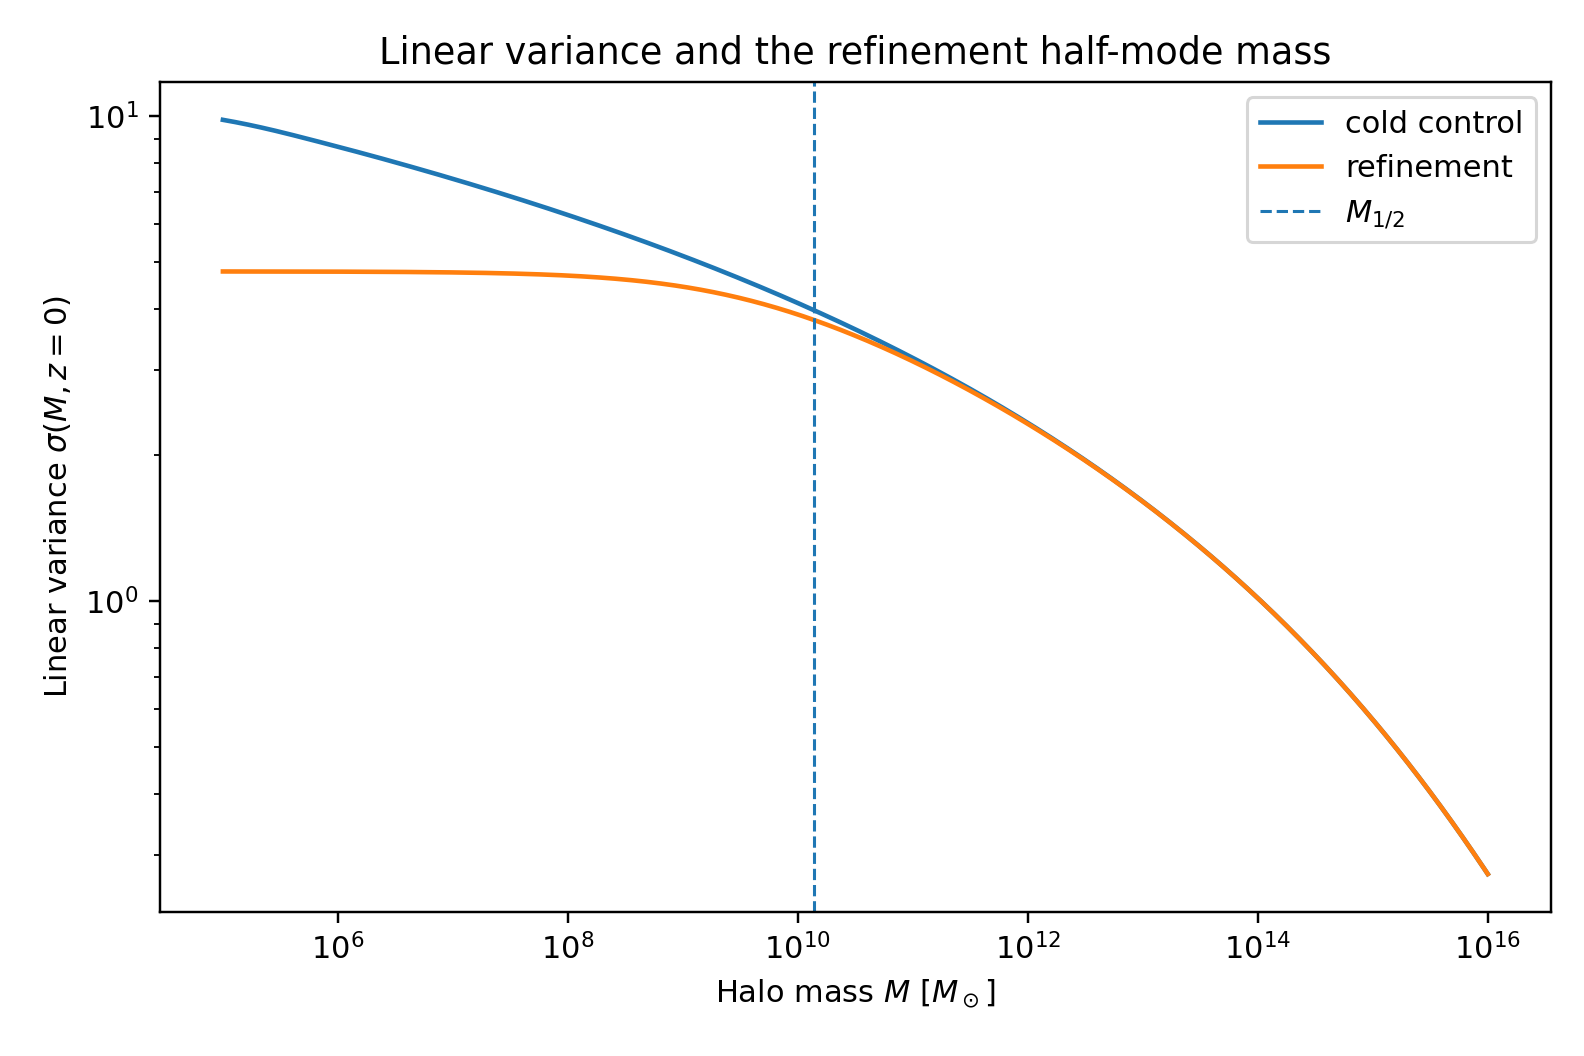
\includegraphics[width=0.86\textwidth]{figures/nls/variance_half_mode.png}
\caption{The linear variance of the cold control and the refinement model.  The ordering is exact within the declared linear spectrum.  The vertical line marks the power half-mode mass.}
\label{fig:nlh-variance}
\end{figure}

\section{Spherical-collapse threshold}

The nonlinear top-hat contrast obeys
\begin{equation}
 \delta''
 +\left(2+\frac{d\log H}{d\log a}\right)\delta'
 -\frac{4}{3}\frac{\delta'^2}{1+\delta}
 -\frac{3}{2}\Omega_m(a)\delta(1+\delta)=0,
 \label{eq:nlh-spherical-collapse}
\end{equation}
where a prime denotes $d/d\log a$.  The initial amplitude is tuned so that the nonlinear solution reaches a declared collapse threshold at the target redshift.  The same initial data are then evolved through the linearized equation, defining $\delta_c(z)$.

The deterministic calculation gives
\begin{equation}
 \delta_c(0)=1.6761139702,
 \qquad
 \delta_c(1)=1.6850426394,
 \qquad
 \delta_c(2)=1.6869970517.
 \label{eq:nlh-delta-c-values}
\end{equation}
The threshold is common to both dark-matter models because their late-time gravitational collapse law is the same.  Their difference enters through $\sigma(M,z)$ and therefore through the abundance of initial peaks.

\section{Excursion-set halo abundance}

The controlled abundance model uses
\begin{equation}
 \frac{dn}{d\log M}
 =\frac{\bar\rho_m}{M}
 f(\nu)
 \left|\frac{d\log\nu}{d\log M}\right|,
 \label{eq:nlh-mass-function}
\end{equation}
with
\begin{equation}
 f(\nu)
 =A_{\rm ST}
 \sqrt{\frac{2a_{\rm ST}}{\pi}}
 \left[1+(a_{\rm ST}\nu^2)^{-p_{\rm ST}}\right]
 \nu e^{-a_{\rm ST}\nu^2/2},
 \label{eq:nlh-st-function}
\end{equation}
where
\begin{equation}
 A_{\rm ST}=0.3222,
 \qquad
 a_{\rm ST}=0.707,
 \qquad
 p_{\rm ST}=0.3.
 \label{eq:nlh-st-parameters}
\end{equation}
These coefficients are a controlled halo-model input, not a derivation from the projector action.

At $z=0$, the refinement-to-cold halo-abundance ratios are
\begin{equation}
 \begin{array}{c|ccccccc}
 M/M_\odot
 &10^7&10^8&10^9&10^{10}&10^{11}&10^{12}&10^{13}\\
 \hline
 (dn/d\log M)_D/(dn/d\log M)_{\rm c}
 &0.0541&0.1746&0.4464&0.7662&0.9335&0.9840&0.9961.
 \end{array}
 \label{eq:nlh-mass-ratios-z0}
\end{equation}
At $z=8$, the corresponding ratios at $10^8$, $10^9$, and $10^{10}M_\odot$ are
\begin{equation}
 \boxed{
 0.0690,
 \qquad
 0.2442,
 \qquad
 0.5544.
 }
 \label{eq:nlh-mass-ratios-z8}
\end{equation}
Thus the cutoff primarily removes low-mass, early-forming halos while leaving cluster-scale abundance nearly unchanged.

\begin{figure}[htbp]
\centering
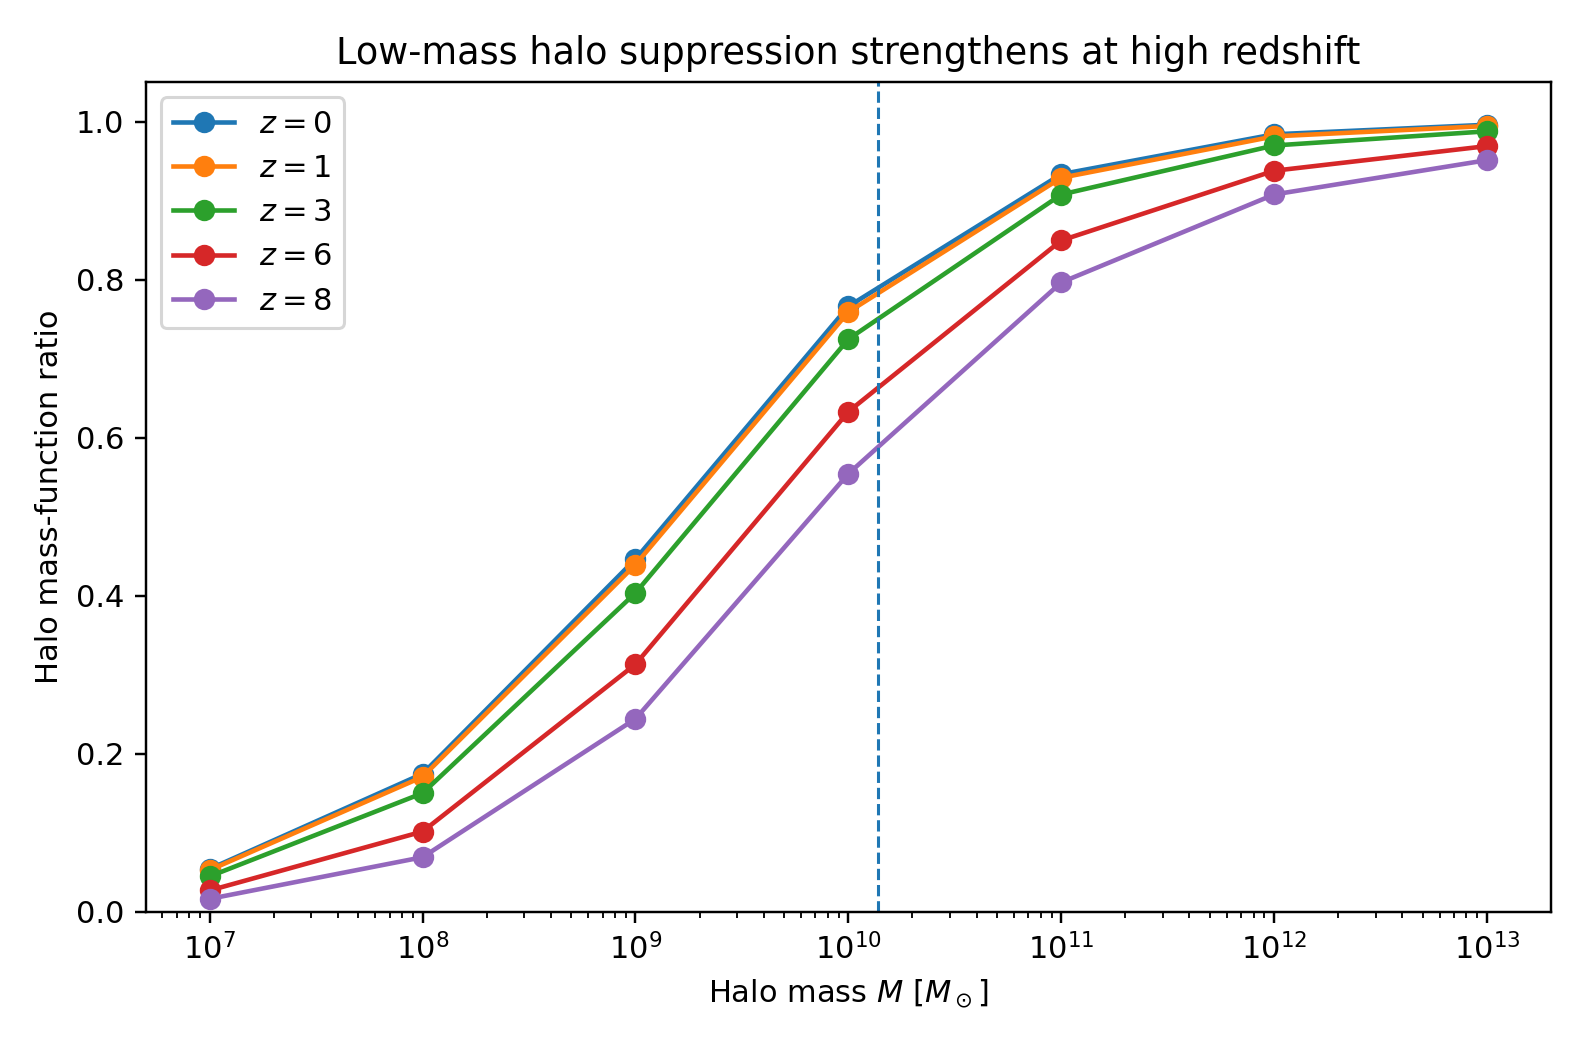
\includegraphics[width=0.86\textwidth]{figures/nls/halo_mass_function_ratios.png}
\caption{Refinement-to-cold halo-abundance ratios in the controlled excursion-set calculation.  The suppression is strongest below the half-mode mass and strengthens toward high redshift.}
\label{fig:nlh-mass-function}
\end{figure}

\section{Formation delay and concentration suppression}

A controlled formation epoch is defined by
\begin{equation}
 D(z_f)\sigma(FM,0)=\delta_{c,\rm EdS},
 \qquad
 F=0.04.
 \label{eq:nlh-formation-redshift}
\end{equation}
The concentration model is
\begin{equation}
 c(M,z)=4\frac{1+z_f}{1+z}.
 \label{eq:nlh-concentration}
\end{equation}
This is used only to propagate the formation delay into a halo-profile template.

At $z=0$,
\begin{equation}
 \begin{array}{c|ccc}
 M/M_\odot
 &10^8&10^{10}&10^{12}\\
 \hline
 z_{f,\rm c}&4.9763&3.2020&1.6202\\
 z_{f,D}&2.5809&2.4305&1.5464\\
 c_D/c_{\rm c}&0.5992&0.8164&0.9718.
 \end{array}
 \label{eq:nlh-concentration-table}
\end{equation}
The refinement cutoff therefore predicts later formation and lower concentrations primarily in low-mass halos.

\section{Compensated nonlinear halo model}

For an NFW profile with normalized Fourier transform $u(k|M)$, define the Lagrangian top-hat window $W(kR_L)$.  The compensated one-halo term is
\begin{equation}
 P_{1h}(k)
 =\int d\log M\,
 \frac{dn}{d\log M}
 \left(\frac{M}{\bar\rho_m}\right)^2
 \left[u(k|M)-W(kR_L)\right]^2.
 \label{eq:nlh-one-halo}
\end{equation}
The subtraction enforces
\begin{equation}
 P_{1h}(k)=O(k^4)
 \label{eq:nlh-one-halo-k4}
\end{equation}
at low wavenumber.  The measured slope is
\begin{equation}
 \boxed{p_{1h}=3.9978690925.}
 \label{eq:nlh-one-halo-slope}
\end{equation}

The normalized two-halo term is
\begin{equation}
 P_{2h}(k)
 =P_{\rm lin}(k)
 \left[
 \frac{
 \int d\log M\,(dn/d\log M)b(M)(M/\bar\rho_m)u(k|M)
 }{
 \int d\log M\,(dn/d\log M)b(M)(M/\bar\rho_m)
 }
 \right]^2.
 \label{eq:nlh-two-halo}
\end{equation}
The total template is
\begin{equation}
 P_{\rm nl}=P_{1h}+P_{2h}.
 \label{eq:nlh-total-power}
\end{equation}

The resulting refinement-to-cold nonlinear ratios are
\begin{equation}
 \begin{array}{c|cccc}
 &k=1&k=10&k=30&k=100\quad [{\rm Mpc}^{-1}]\\
 \hline
 z=0&0.9939&0.9818&0.9556&0.8584\\
 z=1&0.9908&0.9718&0.9225&0.7627\\
 z=2&0.9860&0.9592&0.9048&0.7002.
 \end{array}
 \label{eq:nlh-power-ratios}
\end{equation}
At $k=10\ {\rm Mpc}^{-1}$, the linear power ratio is only
\begin{equation}
 T_D(10)^2=0.3073578289,
 \label{eq:nlh-linear-k10}
\end{equation}
whereas the nonlinear halo-model ratio is
\begin{equation}
 \boxed{
 \frac{P_{\rm nl,D}(10,0)}{P_{\rm nl,c}(10,0)}
 =0.9817480187.
 }
 \label{eq:nlh-nonlinear-k10}
\end{equation}
Halo collapse therefore transfers power back into small physical scales even though the number of low-mass halos is strongly reduced.

\begin{figure}[htbp]
\centering
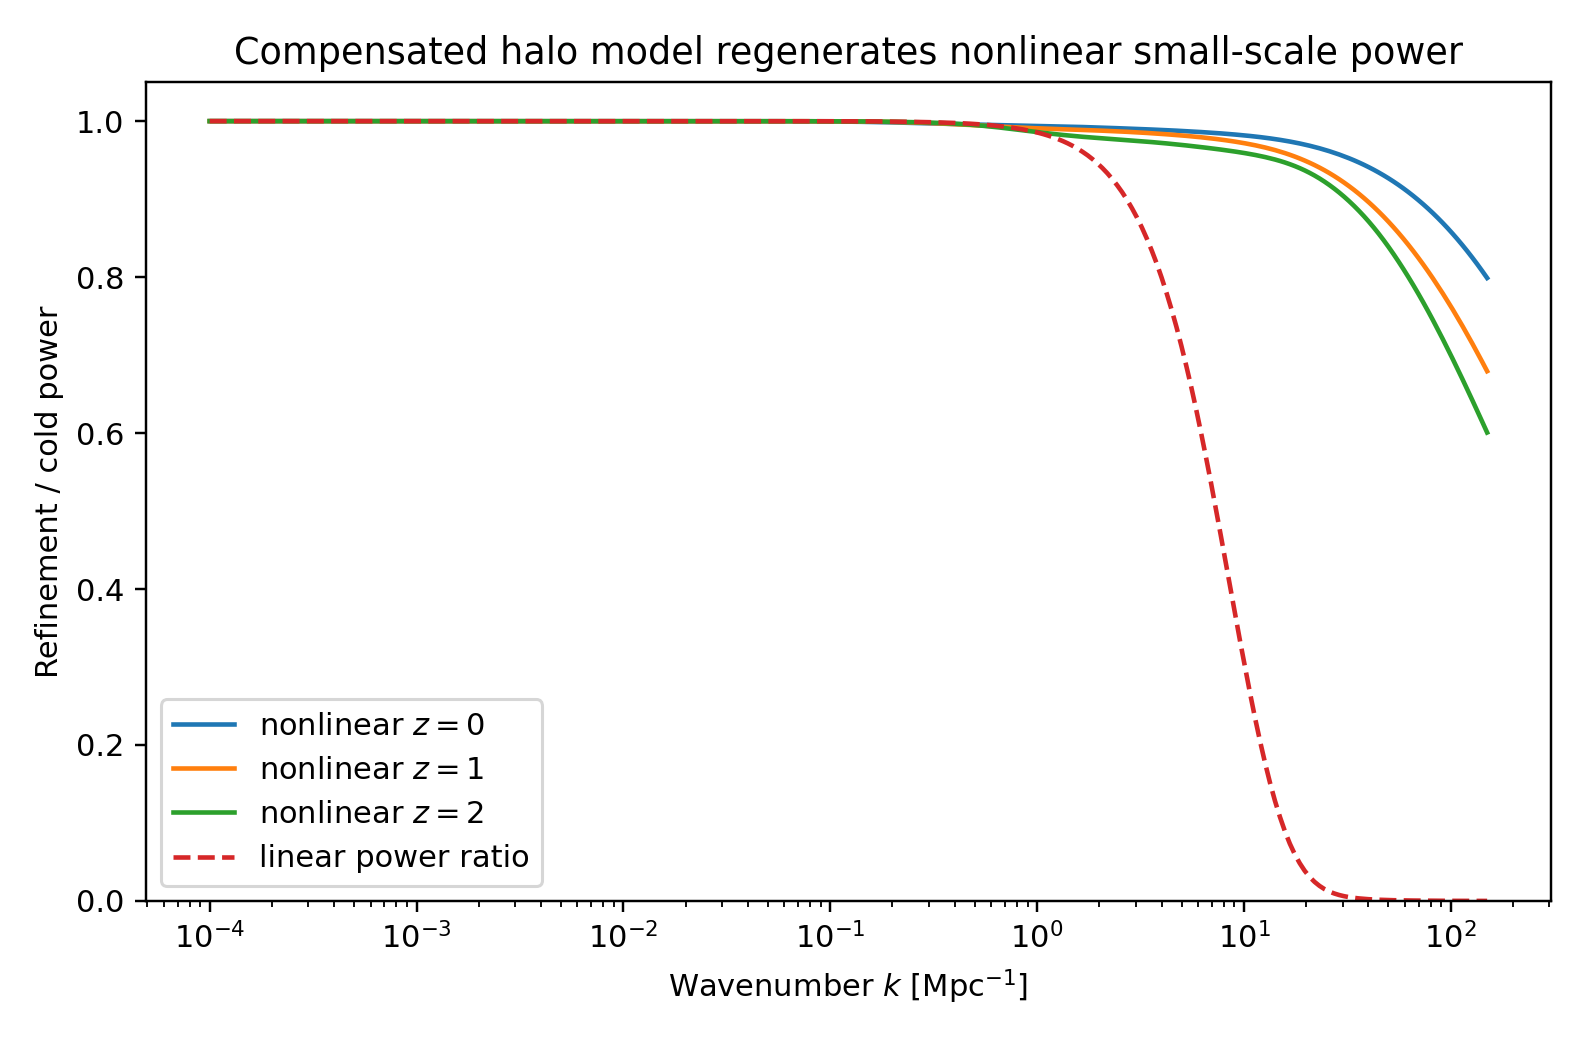
\includegraphics[width=0.88\textwidth]{figures/nls/nonlinear_power_ratios.png}
\caption{The dashed curve is the linear power ratio.  The solid curves are the compensated nonlinear halo-model ratios.  Nonlinear collapse substantially regenerates small-scale power.}
\label{fig:nlh-power}
\end{figure}

\section{Correction to the linear high-multipole lensing forecast}

Projecting the nonlinear halo-model power through a single-source lensing kernel gives the following ratios:
\begin{equation}
 \begin{array}{c|cccc}
 z_s&\ell=1000&\ell=3000&\ell=5000&\ell=10000\\
 \hline
 0.5&0.9926&0.9885&0.9850&0.9770\\
 1.0&0.9938&0.9903&0.9879&0.9826\\
 2.0&0.9953&0.9908&0.9886&0.9843.
 \end{array}
 \label{eq:nlh-nonlinear-lensing}
\end{equation}
The earlier linear calculation gave
\begin{equation}
 \frac{C_{5000,D}^{\kappa\kappa}(z_s=0.5)}
 {C_{5000,\rm c}^{\kappa\kappa}(z_s=0.5)}
 =0.7021280719.
 \label{eq:nlh-linear-lensing-old}
\end{equation}
The nonlinear template instead gives
\begin{equation}
 \boxed{
 \frac{C_{5000,D}^{\kappa\kappa,\rm nl}(z_s=0.5)}
 {C_{5000,\rm c}^{\kappa\kappa,\rm nl}(z_s=0.5)}
 =0.9850165782.
 }
 \label{eq:nlh-nonlinear-lensing-new}
\end{equation}
Therefore the strong linear high-$\ell$ suppression is superseded as a final forecast.  In this controlled halo model, nonlinear structure largely erases it.  Baryonic feedback and a calibrated nonlinear emulator remain necessary before a precision lensing claim can be made.

\begin{figure}[htbp]
\centering
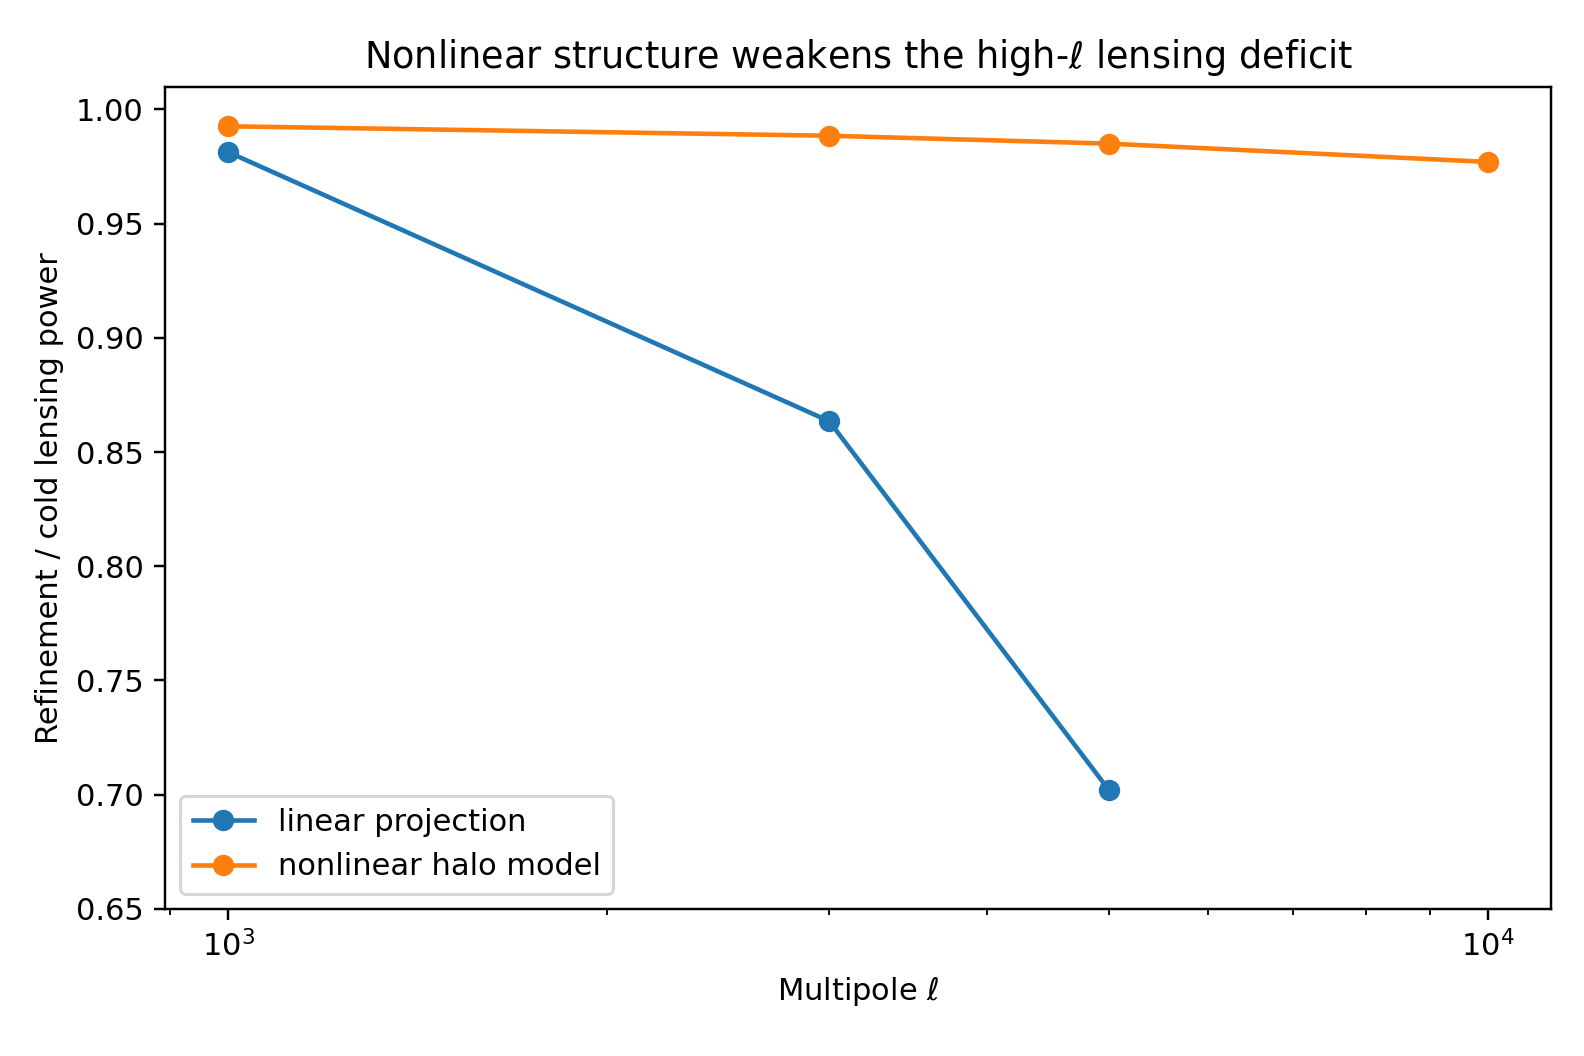
\includegraphics[width=0.84\textwidth]{figures/nls/linear_vs_nonlinear_lensing.png}
\caption{The earlier linear projection and the present nonlinear halo-model projection for $z_s=0.5$.  Nonlinear power regeneration removes most of the large linear high-$\ell$ deficit.}
\label{fig:nlh-lensing-correction}
\end{figure}

\section{Reionization consistency}

Use the declared atomic-cooling threshold
\begin{equation}
 M_{\rm atom}(z)
 =10^8M_\odot
 \left(\frac{1+z}{10}\right)^{-3/2}.
 \label{eq:nlh-atomic-mass}
\end{equation}
The collapsed fraction is
\begin{equation}
 f_{\rm coll}(>M,z)
 =\frac{1}{\bar\rho_m}
 \int_M^\infty
 M'\frac{dn}{d\log M'}\,d\log M'.
 \label{eq:nlh-collapsed-fraction}
\end{equation}
If a simple ionization model has $Q_{\rm HII}\propto\zeta_{\rm ion}f_{\rm coll}$, the same ionization history requires
\begin{equation}
 \boxed{
 \frac{\zeta_{\rm ion,D}}{\zeta_{\rm ion,c}}
 =\frac{f_{\rm coll,c}}{f_{\rm coll,D}}.
 }
 \label{eq:nlh-efficiency-penalty}
\end{equation}

The controlled results are
\begin{equation}
 \begin{array}{c|cccc}
 z&6.0&7.4&8.0&10.0\\
 \hline
 f_{\rm coll,D}/f_{\rm coll,c}
 &0.4673&0.3423&0.2944&0.1661\\
 \zeta_D/\zeta_{\rm c}
 &2.1400&2.9216&3.3973&6.0212.
 \end{array}
 \label{eq:nlh-reionization-table}
\end{equation}
At the calibrated reionization midpoint $z\simeq7.4$, the current benchmark therefore requires approximately three times the ionizing efficiency of the cold control.

\begin{figure}[htbp]
\centering
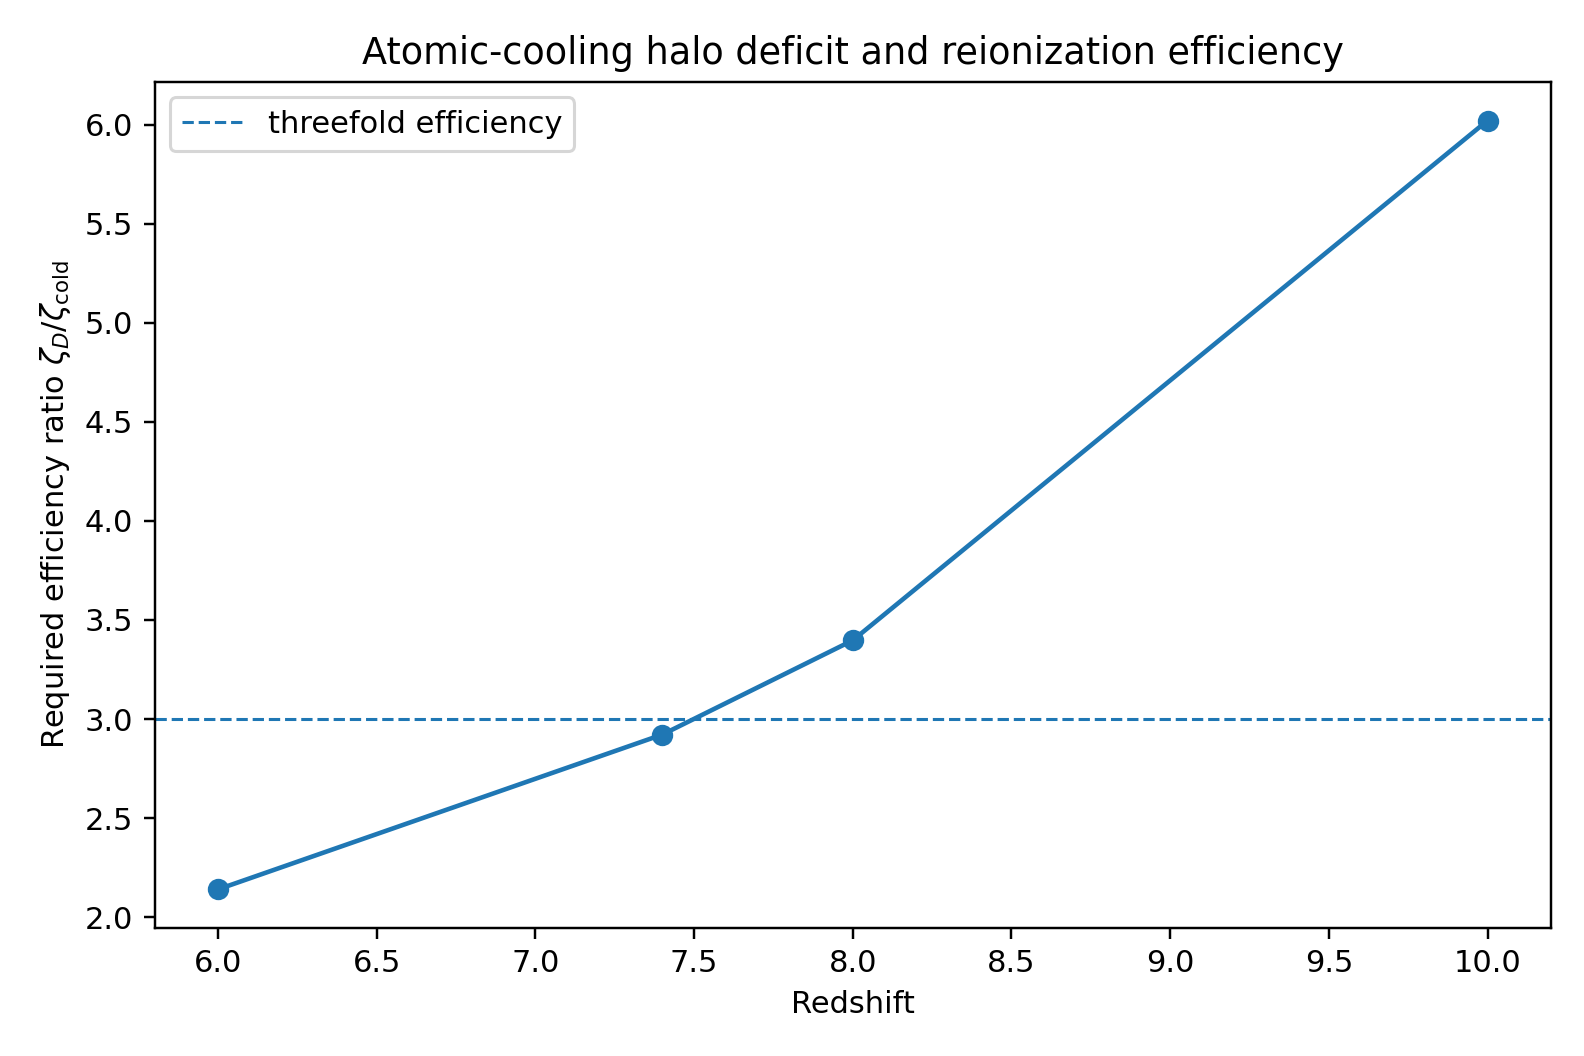
\includegraphics[width=0.82\textwidth]{figures/nls/reionization_efficiency_penalty.png}
\caption{Required ionizing-efficiency ratio in the atomic-cooling halo model.  The present cutoff produces a substantial high-redshift halo deficit.}
\label{fig:nlh-reionization}
\end{figure}

\subsection{Production-epoch bound}

The scale-covariant cutoff obeys the approximate scaling
\begin{equation}
 k_{1/2}\propto a_\star^{-1}.
 \label{eq:nlh-cutoff-scaling}
\end{equation}
Rescaling the fixed transfer while holding the remaining background inputs unchanged gives
\begin{equation}
 \begin{array}{c|cccc}
 \text{maximum efficiency penalty}
 &1.5&2&3&5\\
 \hline
 a_{\star,\max}
 &4.67\times10^{-7}
 &6.95\times10^{-7}
 &1.02\times10^{-6}
 &1.46\times10^{-6}\\
 k_{1/2,\min}\ [{\rm Mpc}^{-1}]
 &15.74&10.58&7.19&5.04.
 \end{array}
 \label{eq:nlh-production-bounds}
\end{equation}
The benchmark $a_\star=10^{-6}$ therefore lies close to the boundary of a threefold efficiency penalty.  Earlier production would move the cutoff to smaller spatial scales and ease the reionization burden.

\section{Verification}

The deterministic audit records
\begin{equation}
 \boxed{
 24\ {\rm PASS},
 \qquad
 0\ {\rm FAIL}.
 }
 \label{eq:nlh-pass-count}
\end{equation}
Selected controls are
\begin{equation}
 \begin{array}{c|c}
 \text{control}&\text{residual or discrepancy}\\
 \hline
 \sigma_8\ \text{reconstruction}&0\\
 T_D(k_{1/2})^2-1/2&1.11\times10^{-16}\\
 \text{one-halo low-}k\text{ slope error}&2.13\times10^{-3}\\
 \text{mass-grid refinement}&3.31\times10^{-5}\\
 \text{lensing-grid refinement}&2.89\times10^{-6}.
 \end{array}
 \label{eq:nlh-verification-table}
\end{equation}

\section{Claim boundary and resulting direction}

This chapter is a controlled semi-analytic nonlinear closure.  It does not establish:
\begin{itemize}
 \item a first-principles halo mass function from the projector action;
 \item calibrated halo concentrations or subhalo disruption;
 \item hydrodynamics, star formation, feedback, or metal enrichment;
 \item nonlinear Vlasov evolution from the production surface;
 \item a precision nonlinear matter emulator;
 \item a galaxy survey, reionization, or lensing likelihood;
 \item observational correctness or literature priority.
\end{itemize}

The robust result is not the exact numerical value of the halo-model lensing ratio.  It is the separation
\begin{equation}
 \boxed{
 \begin{aligned}
 \text{linear and high-redshift statistics}
 &:\ \text{strong cutoff sensitivity},\\
 \text{deeply nonlinear projected power}
 &:\ \text{substantial gravitational regeneration}.
 \end{aligned}}
 \label{eq:nlh-observable-separation}
\end{equation}
A full nonlinear test therefore requires a particle or phase-space solver with baryonic source terms, followed by a frozen-parameter likelihood using the low-mass halo abundance, reionization history, CMB lensing, and galaxy lensing together.
\chapter{Paired Three-Dimensional Particle--Mesh Nonlinear Refinement}
\label{ch:paired-pm-nonlinear}

\section{Scope and objective}

The preceding nonlinear-structure chapter propagated the collisionless refinement transfer through spherical collapse, a halo mass function, a compensated halo model, and reionization consistency.  That calculation found that nonlinear halo formation can regenerate much of the linearly suppressed small-scale power, while low-mass halo abundance and formation time remain more strongly altered.  The result was model based rather than a direct phase-space evolution.

This chapter supplies an independent test.  It evolves paired cold and refinement initial conditions with the same random phases in a three-dimensional cosmological particle--mesh system.  The calculation is designed to answer three narrow questions:
\begin{enumerate}[leftmargin=2em]
\item Does direct nonlinear evolution regenerate the suppressed refinement power?
\item Does delayed high-density collapse remain visible after that regeneration?
\item Does an independent particle calculation agree with the preceding halo-model trend?
\end{enumerate}

The answer to all three questions is affirmative in the declared finite box.  The calculation is a controlled particle--mesh benchmark.  It is not a precision $N$-body simulation, a resolved subhalo catalog, or an observational likelihood.

\section{Paired initial conditions}

Let $P_{\rm c}(k)$ denote the cold linear power normalized to $\sigma_8=0.81$.  The refinement branch uses the previously derived collisionless transfer amplitude $T_D(k)$,
\begin{equation}
 P_D(k)=T_D(k)^2P_{\rm c}(k),
 \qquad 0\leq T_D(k)\leq1.
 \label{eq:pm-paired-linear-power}
\end{equation}
The same Gaussian white-noise realization is used in both branches.  Thus every retained Fourier mode has the same initial phase.  Before nonlinear evolution,
\begin{equation}
 r_{\rm cD}(k)
 :=
 \frac{P_{\rm cD}(k)}{\sqrt{P_{\rm c}(k)P_D(k)}}=1,
 \label{eq:pm-initial-cross-correlation}
\end{equation}
and the only difference is the deterministic amplitude factor $T_D(k)$.

The Zel'dovich map is
\begin{equation}
 \boldsymbol x(\boldsymbol q,a_i)
 =
 \boldsymbol q+D(a_i)\boldsymbol s(\boldsymbol q),
 \label{eq:pm-zeldovich-position}
\end{equation}
\begin{equation}
 \boldsymbol p(\boldsymbol q,a_i)
 =
 a_i^2H(a_i)f(a_i)D(a_i)\boldsymbol s(\boldsymbol q),
 \label{eq:pm-zeldovich-momentum}
\end{equation}
where
\begin{equation}
 \boldsymbol s_{\boldsymbol k}
 =
 i\frac{\boldsymbol k}{k^2}\delta_{0,\boldsymbol k},
 \qquad
 f=\frac{d\log D}{d\log a}.
 \label{eq:pm-zeldovich-displacement}
\end{equation}
The background uses
\begin{equation}
 E(a)^2
 =
 \Omega_{r0}a^{-4}
 +\Omega_{m0}a^{-3}
 +\Omega_{V0},
 \label{eq:pm-background}
\end{equation}
with
\begin{equation}
 \Omega_{m0}=0.31,
 \qquad
 \Omega_{r0}=9\times10^{-5},
 \qquad
 \Omega_{V0}=0.68991.
 \label{eq:pm-background-values}
\end{equation}

\section{Particle--mesh evolution}

In comoving coordinates,
\begin{equation}
 \ddot{\boldsymbol x}+2H\dot{\boldsymbol x}
 =
 -\frac{1}{a^2}\nabla_x\Phi,
 \label{eq:pm-comoving-equation}
\end{equation}
\begin{equation}
 \nabla_x^2\Phi
 =
 \frac32\Omega_{m0}H_0^2a^{-1}\delta.
 \label{eq:pm-poisson}
\end{equation}
Define the canonical momentum
\begin{equation}
 \boldsymbol p=a^2\dot{\boldsymbol x}.
 \label{eq:pm-canonical-momentum}
\end{equation}
Using the scale factor as time gives
\begin{equation}
 \frac{d\boldsymbol x}{da}
 =
 \frac{\boldsymbol p}{a^3H},
 \label{eq:pm-drift-equation}
\end{equation}
\begin{equation}
 \frac{d\boldsymbol p}{da}
 =
 \frac{3\Omega_{m0}H_0^2}{2a^2H}
 \nabla\nabla^{-2}\delta.
 \label{eq:pm-kick-equation}
\end{equation}

Cloud-in-cell deposition defines the mesh density.  The Fourier-space mesh force is
\begin{equation}
 \boldsymbol F_{\boldsymbol k}
 =
 i\frac{\boldsymbol k}{k^2}\delta_{\boldsymbol k},
 \qquad \boldsymbol F_{\boldsymbol 0}=0.
 \label{eq:pm-spectral-force}
\end{equation}
The same cloud-in-cell kernel interpolates the force back to the particles.  This symmetric assignment keeps the net force and total canonical momentum at roundoff.

The kick--drift--kick factors are evaluated by Gaussian quadrature,
\begin{equation}
 K(a_1,a_2)
 =
 \frac32\Omega_{m0}
 \int_{a_1}^{a_2}
 \frac{da}{a^2E(a)},
 \label{eq:pm-kick-factor}
\end{equation}
\begin{equation}
 D_{\rm drift}(a_1,a_2)
 =
 \int_{a_1}^{a_2}
 \frac{da}{a^3E(a)}.
 \label{eq:pm-drift-factor}
\end{equation}

\section{Numerical realization}

The main paired calculation uses
\begin{equation}
 N_g=64,
 \qquad
 N_p=64^3=262144,
 \label{eq:pm-main-resolution}
\end{equation}
\begin{equation}
 L=14.2857142857\ {\rm Mpc},
 \qquad
 \Delta x=0.2232142857\ {\rm Mpc},
 \label{eq:pm-box}
\end{equation}
\begin{equation}
 a_i=0.02,
 \qquad
 N_{\rm step}=80.
 \label{eq:pm-time-resolution}
\end{equation}
The particle mass is
\begin{equation}
 m_p
 =
 \bar\rho_m\frac{L^3}{N_p}
 =
 4.6886092251\times10^8\ M_\odot.
 \label{eq:pm-particle-mass}
\end{equation}
The deconvolved power analysis retains
\begin{equation}
 k<0.65k_{\rm Ny}
 =9.1483178073\ {\rm Mpc}^{-1}.
 \label{eq:pm-usable-k}
\end{equation}
The input power half-mode is
\begin{equation}
 k_{1/2}=7.3571107668\ {\rm Mpc}^{-1},
 \label{eq:pm-input-half-mode}
\end{equation}
so the main mesh resolves the declared cutoff region.

\section{Nonlinear power regeneration}

For each snapshot define
\begin{equation}
 R_P(k,a)
 :=
 \frac{P_D^{\rm PM}(k,a)}{P_{\rm c}^{\rm PM}(k,a)}.
 \label{eq:pm-power-ratio}
\end{equation}
At $k=8\ {\rm Mpc}^{-1}$, the input linear ratio is
\begin{equation}
 T_D(8)^2=0.4474940507.
 \label{eq:pm-k8-input}
\end{equation}
The measured paired ratios are
\begin{align}
 R_P(8,0.05)&=0.5236906387,\label{eq:pm-k8-a005}\\
 R_P(8,0.10)&=0.6336086860,\label{eq:pm-k8-a01}\\
 R_P(8,0.25)&=0.9082585376,\label{eq:pm-k8-a025}\\
 R_P(8,0.50)&=0.9567667002,\label{eq:pm-k8-a05}\\
 R_P(8,1)&=0.9918100525.\label{eq:pm-k8-a1}
\end{align}
At the input half-mode,
\begin{equation}
 R_P(k_{1/2},1)=0.9928833783.
 \label{eq:pm-halfmode-final}
\end{equation}
The direct particle evolution therefore confirms the earlier conclusion:
\begin{equation}
 \boxed{
 \text{nonlinear mode coupling regenerates most of the linearly suppressed power by }a=1.
 }
 \label{eq:pm-regeneration-conclusion}
\end{equation}

\begin{figure}[htbp]
\centering
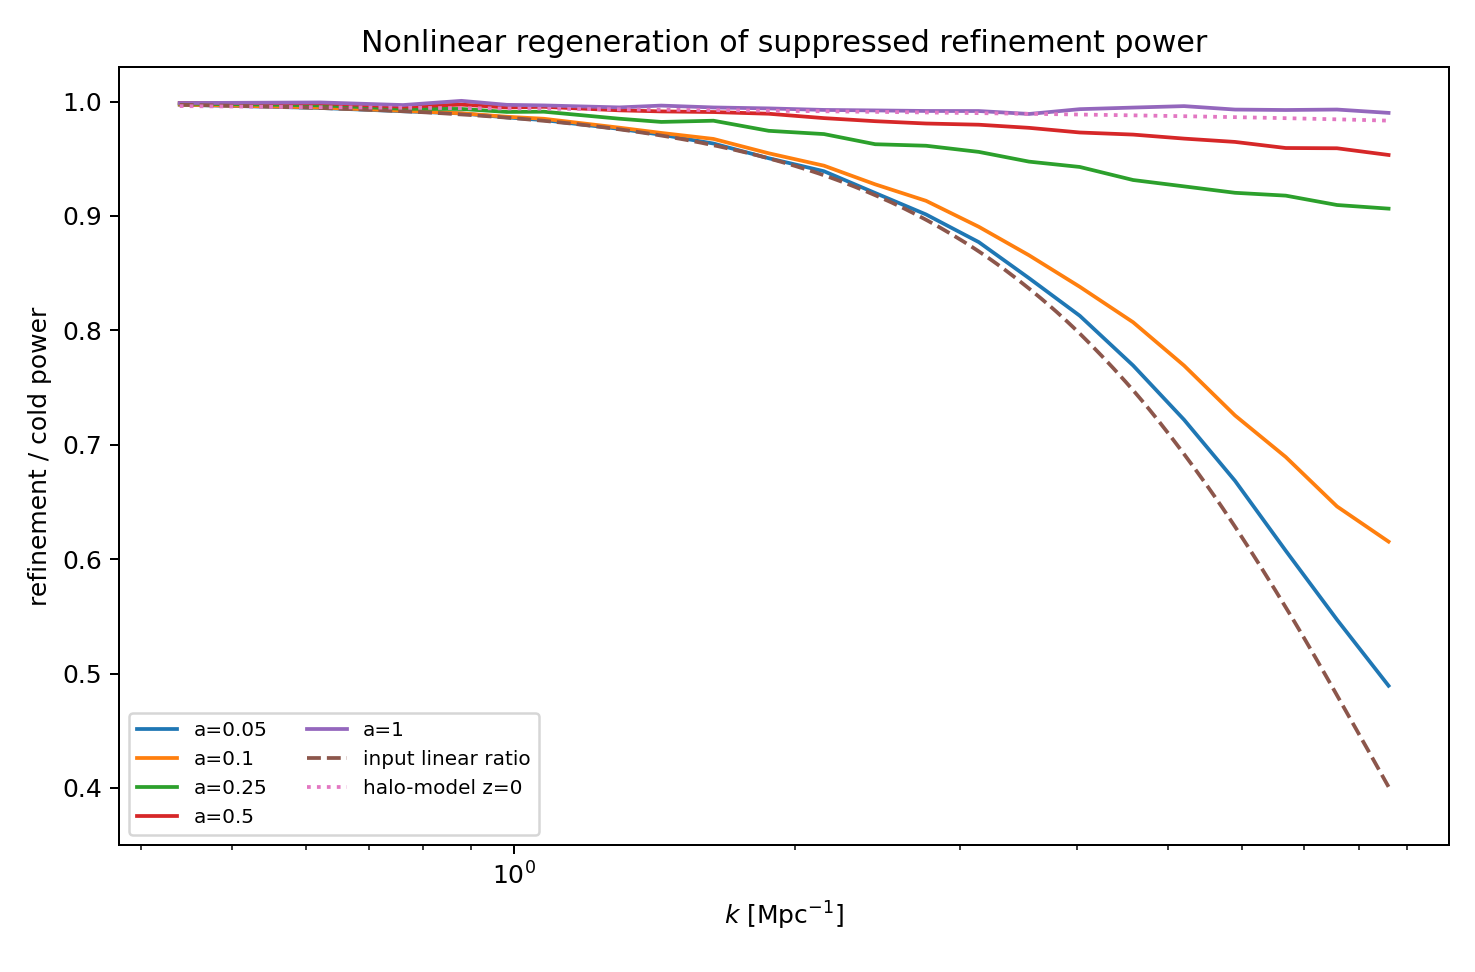
\includegraphics[width=0.95\linewidth]{figures/pm/01_power_regeneration.png}
\caption{Paired nonlinear power ratios.  The early evolution retains the linear cutoff.  The ratio approaches unity as nonlinear mode coupling transfers power into the suppressed band.  The independent halo-model result has the same late-time trend.}
\label{fig:pm-power-regeneration}
\end{figure}

Selected values are collected below.
\begin{center}
\begin{tabular}{rrrrr}
\toprule
$k\,[{\rm Mpc}^{-1}]$ & input $T_D^2$ & $R_P(a=0.05)$ & $R_P(a=0.25)$ & $R_P(a=1)$\\
\midrule
4.00 & 0.79954 & 0.81467 & 0.94307 & 0.99307\\
6.00 & 0.61937 & 0.66078 & 0.91991 & 0.99292\\
7.35 & 0.50060 & 0.56281 & 0.91169 & 0.99288\\
8.00 & 0.44749 & 0.52369 & 0.90826 & 0.99181\\
9.00 & 0.37277 & 0.48933 & 0.90637 & 0.99008\\
\bottomrule
\end{tabular}
\end{center}

\section{Phase coherence of the nonlinear cosmic web}

The paired cross-correlation is
\begin{equation}
 r_{\rm cD}(k,a)
 =
 \frac{P_{\rm cD}(k,a)}{
 \sqrt{P_{\rm c}(k,a)P_D(k,a)}}.
 \label{eq:pm-cross-correlation}
\end{equation}
At $k=8\ {\rm Mpc}^{-1}$,
\begin{equation}
 r_{\rm cD}(8,1)=0.9981981720.
 \label{eq:pm-k8-cross}
\end{equation}
Across the retained $a=1$ modes,
\begin{equation}
 \min_k r_{\rm cD}(k,1)=0.9978380.
 \label{eq:pm-min-cross}
\end{equation}
The large-scale skeleton and most nonlinear structures therefore remain paired.  The refinement branch alters collapse timing and internal density more strongly than it relocates the cosmic web.

\begin{figure}[htbp]
\centering
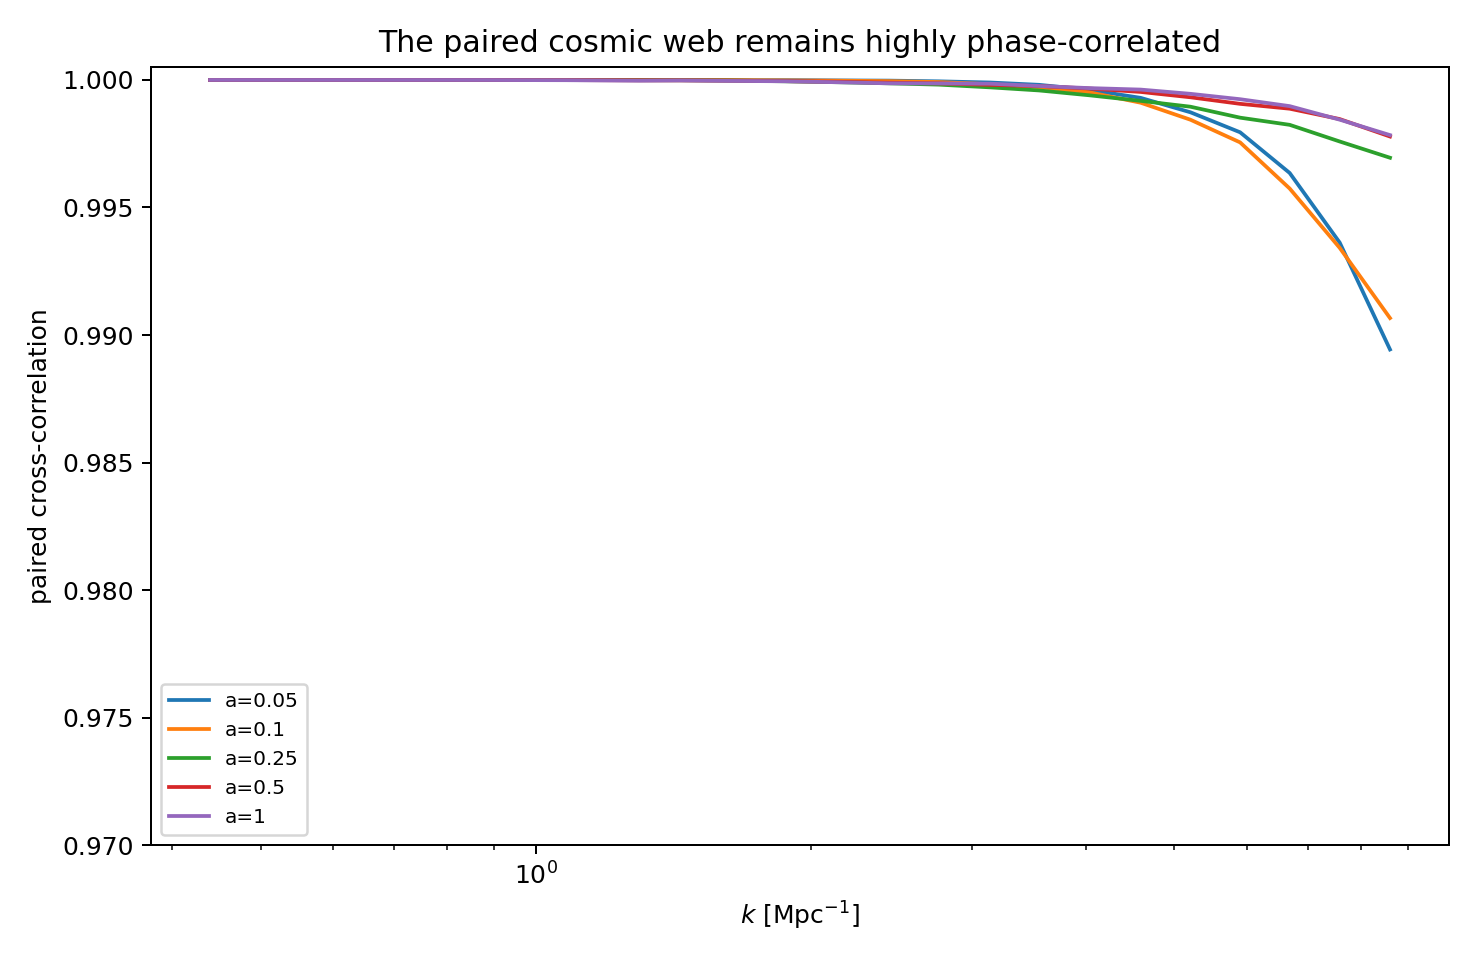
\includegraphics[width=0.95\linewidth]{figures/pm/03_cross_correlation.png}
\caption{Cross-correlation of the paired density fields.  The phases remain highly correlated even after nonlinear power has been regenerated.}
\label{fig:pm-cross-correlation}
\end{figure}

\begin{figure}[htbp]
\centering
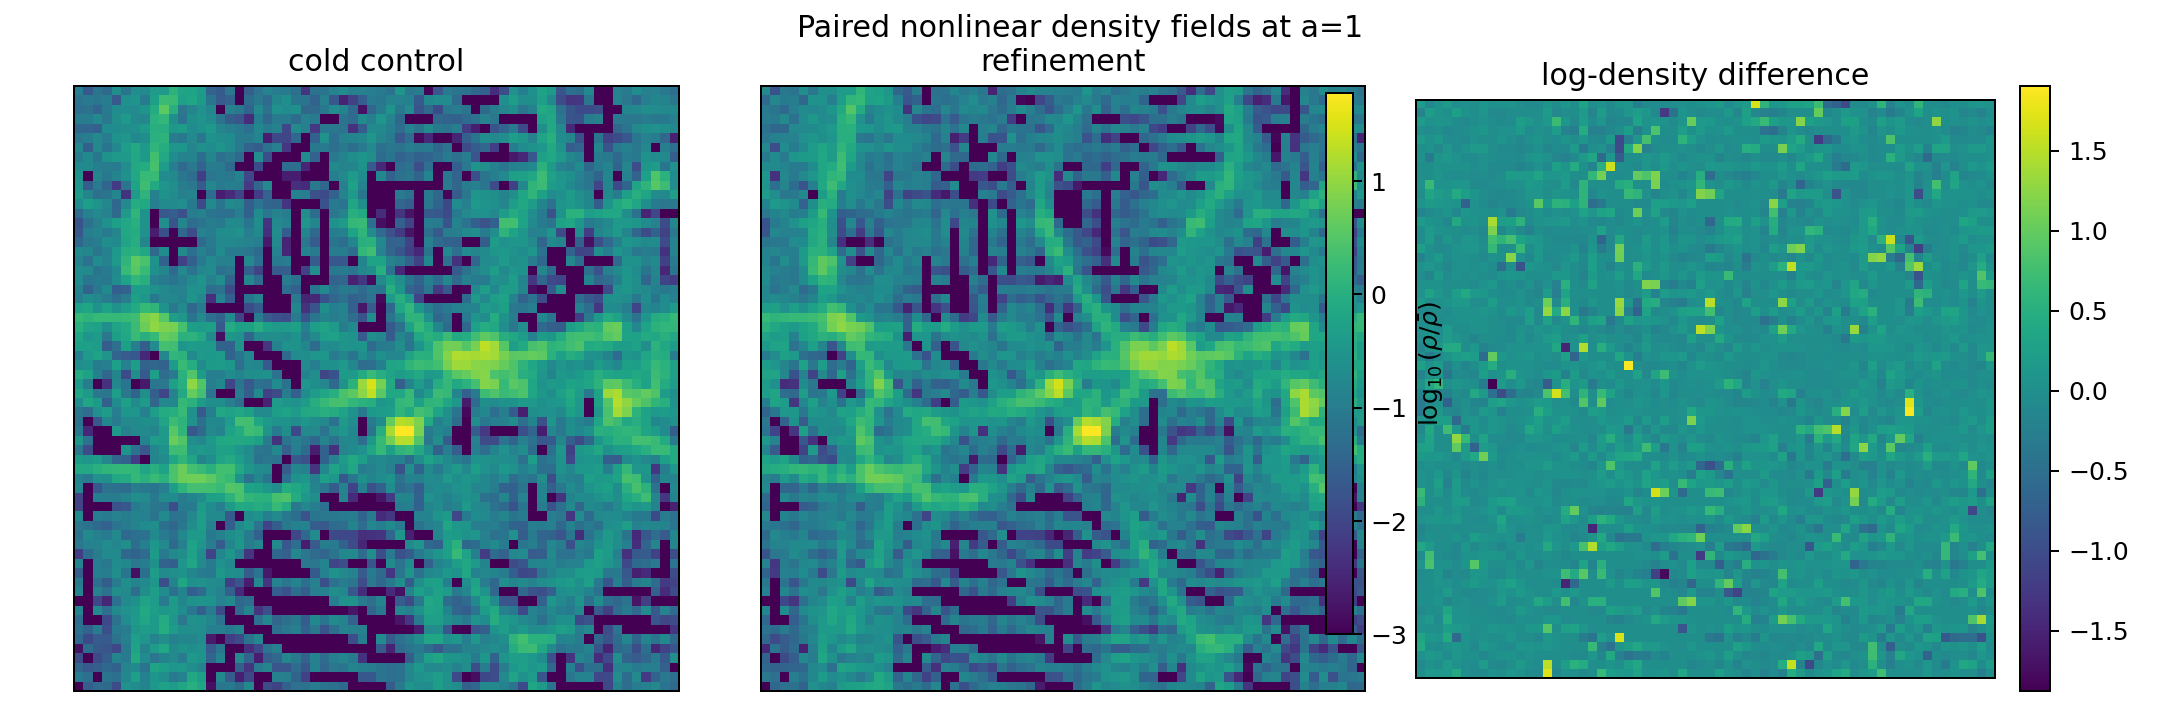
\includegraphics[width=\linewidth]{figures/pm/04_density_slices.png}
\caption{Four-cell slab averages of the paired $a=1$ density fields.  The same filaments and nodes appear in both branches, while the difference map isolates changes in local collapse and internal density.}
\label{fig:pm-density-slices}
\end{figure}

\section{Delayed high-density collapse}

For a mesh density threshold $\Delta_\rho$, define the mass fraction
\begin{equation}
 F_M(>\Delta_\rho,a)
 =
 \frac{
 \sum_{j:\rho_j/\bar\rho>\Delta_\rho}\rho_j
 }{
 \sum_j\rho_j
 }.
 \label{eq:pm-collapsed-mass-fraction}
\end{equation}
A local mesh maximum above the same threshold is counted as a peak proxy.  These are not halo catalogs.  They provide a direct, resolution-declared collapse diagnostic.

At $a=0.25$, corresponding to $z=3$, the threshold $\rho/\bar\rho>20$ gives
\begin{equation}
 \frac{F_{M,D}}{F_{M,\rm c}}=0.9045351965,
 \label{eq:pm-z3-mass-ratio}
\end{equation}
\begin{equation}
 \frac{N_{{\rm peak},D}}{N_{{\rm peak},\rm c}}=0.8551724138.
 \label{eq:pm-z3-peak-ratio}
\end{equation}
At $a=1$, the corresponding ratios are
\begin{equation}
 \frac{F_{M,D}}{F_{M,\rm c}}=0.9745091917,
 \qquad
 \frac{N_{{\rm peak},D}}{N_{{\rm peak},\rm c}}=0.8962962963.
 \label{eq:pm-z0-collapse-ratios}
\end{equation}
Power regeneration is therefore more complete than collapse-statistic regeneration.

\begin{figure}[htbp]
\centering
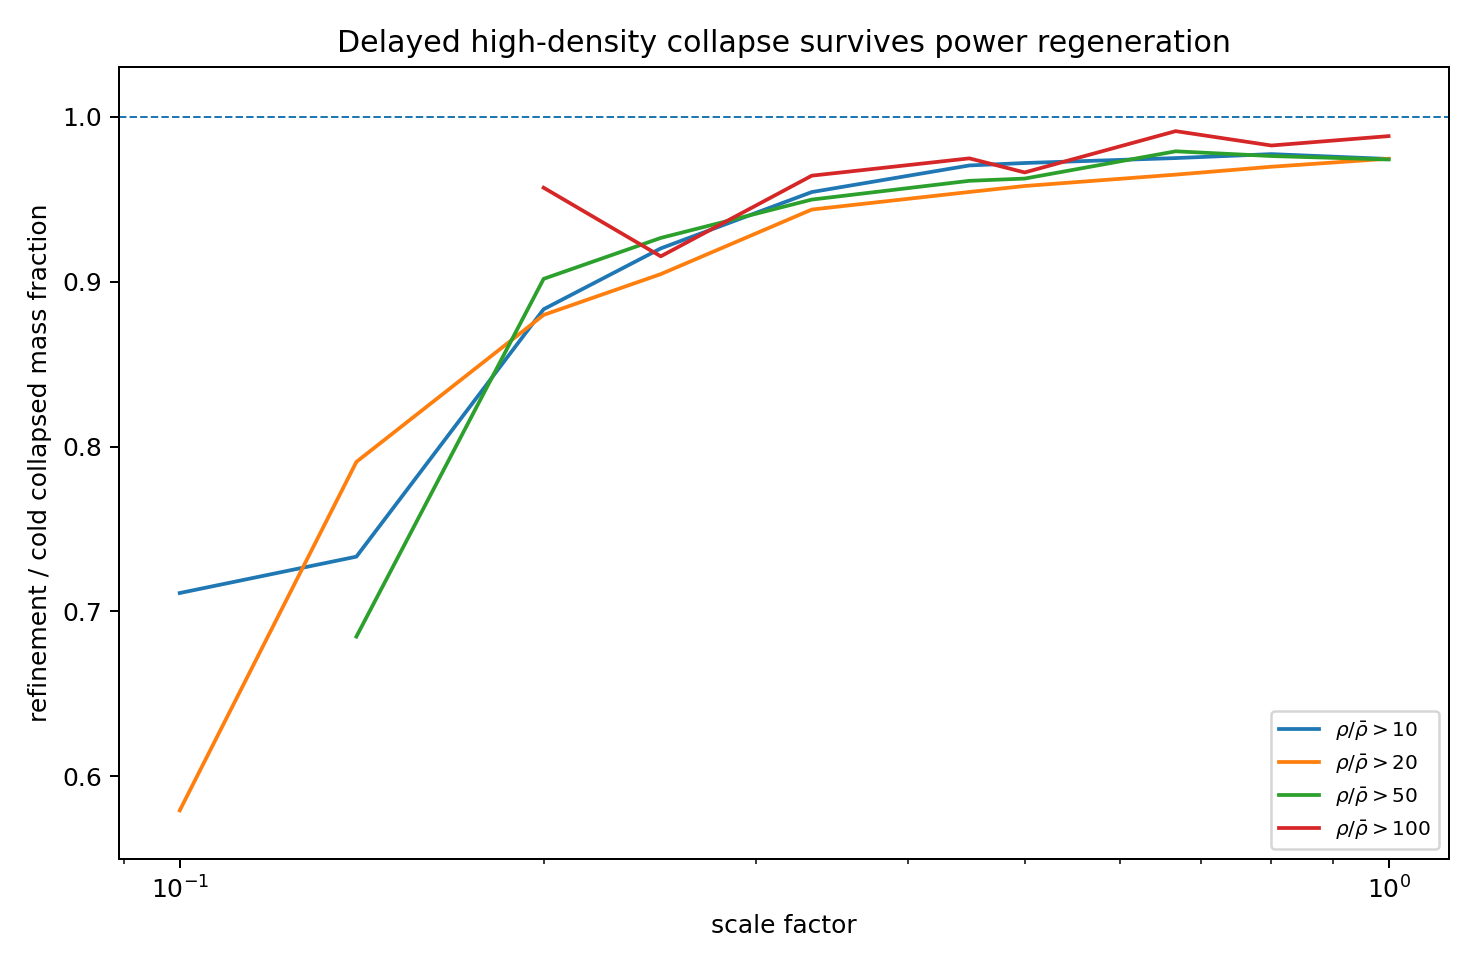
\includegraphics[width=0.95\linewidth]{figures/pm/02_collapsed_mass_fraction.png}
\caption{Ratio of refinement to cold mass above fixed mesh-density thresholds.  The largest delay occurs during the onset of nonlinear collapse.  The ratios approach unity at late times but do not become exactly equal.}
\label{fig:pm-collapsed-fraction}
\end{figure}

For selected target mass fractions, the interpolation gives:
\begin{center}
\begin{tabular}{rrrrr}
\toprule
threshold & target $F_M$ & $a_{\rm c}$ & $a_D$ & delay $a_D/a_{\rm c}-1$\\
\midrule
10 & 0.25 & 0.29540 & 0.30615 & 0.03641\\
20 & 0.10 & 0.24093 & 0.25122 & 0.04270\\
50 & 0.10 & 0.33546 & 0.34352 & 0.02405\\
100 & 0.05 & 0.32301 & 0.32749 & 0.01386\\
\bottomrule
\end{tabular}
\end{center}
Thus the controlled formation delay is of order one to four percent in scale factor for these mesh thresholds.

\section{Independent comparison with the halo-model closure}

The preceding compensated halo model predicted a mild $z=0$ nonlinear suppression despite a strong linear cutoff.  The particle--mesh and halo-model ratios are independent constructions.  Their root-mean-square difference over the common retained modes is
\begin{equation}
 \boxed{
 \epsilon_{\rm PM/HM}=4.6838158064\times10^{-3}.
 }
 \label{eq:pm-halo-rms}
\end{equation}
At $k=8\ {\rm Mpc}^{-1}$,
\begin{equation}
 R_P^{\rm PM}=0.9918100525,
 \qquad
 R_P^{\rm halo}=0.9839760245.
 \label{eq:pm-halo-k8}
\end{equation}
The agreement is not a proof that either approximation is precision accurate.  It is a nontrivial cross-method confirmation of the same qualitative conclusion:
\begin{equation}
 \boxed{
 \begin{gathered}
 \text{late-time power can nearly recover,}\\
 \text{while halo and peak statistics retain a stronger memory of the cutoff.}
 \end{gathered}
 }
 \label{eq:pm-cross-method-conclusion}
\end{equation}

\section{Verification and convergence}

The deterministic audit records
\begin{equation}
 \boxed{20\ {\rm PASS},\qquad0\ {\rm FAIL}.}
 \label{eq:pm-audit-total}
\end{equation}
Selected controls are:
\begin{center}
\begin{tabular}{lr}
\toprule
control & residual or discrepancy\\
\midrule
mass conservation & $4.16\times10^{-17}$\\
maximum mean net force & $4.31\times10^{-15}$\\
relative total-momentum residual & $7.21\times10^{-16}$\\
linear plane-wave growth error & $7.49\times10^{-3}$\\
grid-control ratio discrepancy & $1.67\times10^{-2}$\\
time-step ratio discrepancy & $1.11\times10^{-3}$\\
paired-phase fractional scatter & $2.79\times10^{-3}$\\
PM versus halo-model RMS difference & $4.68\times10^{-3}$\\
\bottomrule
\end{tabular}
\end{center}
The $48^3$ grid control and the 96-step time control preserve the paired ratios within the declared tolerances.  Two independent paired-phase runs on a smaller grid give sub-percent ratio scatter.

\section{Physical interpretation}

The direct particle calculation changes the emphasis of the refinement prediction.

First, a large suppression in the linear transfer does not imply an equally large suppression in the fully nonlinear matter power.  Mode coupling and collapse repopulate the high-$k$ band.

Second, the initial cutoff still has measurable dynamical consequences.  High-density regions appear later, contain slightly less mass, and contain fewer mesh peaks.  These effects are strongest during early nonlinear formation and persist weakly to the present.

Third, the paired fields remain almost perfectly phase correlated.  The candidate model predicts a familiar large-scale cosmic web with altered low-mass and internal structure, rather than a radically relocated web.

The strongest controlled conclusion is therefore
\begin{equation}
 \boxed{
 \begin{gathered}
 \text{linear cutoff}\
 \Downarrow\\
 \text{delayed early collapse and fewer dense peaks}\
 \Downarrow\\
 \text{nonlinear high-}k\text{ power regeneration}\
 \Downarrow\\
 \text{late-time power nearly cold, but formation memory remains}.
 \end{gathered}
 }
 \label{eq:pm-physical-chain}
\end{equation}

\section{Claim boundary}

The calculation has several explicit limitations.
\begin{itemize}[leftmargin=2em]
\item The box is $14.29\ {\rm Mpc}$ on a side and omits long-wavelength sample variance.
\item The force is particle--mesh with a $0.223\ {\rm Mpc}$ cell.  Halo cores and subhalos are unresolved.
\item The particle mass is $4.69\times10^8M_\odot$.  The run cannot directly test the smallest halo masses in the analytic mass-function calculation.
\item The initial conditions use the Zel'dovich approximation rather than a production-grade second-order generator.
\item There is no baryonic gas, cooling, star formation, feedback, or radiation transport.
\item The mesh peak statistic is not a friends-of-friends or spherical-overdensity halo finder.
\item One finite box does not establish a converged cosmological prediction.
\end{itemize}

The result is therefore a controlled nonlinear phase-space benchmark, not a final simulation campaign.
\chapter{Paired Multi-Box Refinement Halo Catalogues}
\label{ch:paired-halo-catalogues}

\section{Scope and objective}

The preceding nonlinear structure calculation established a nonlinear Vlasov--Poisson limit, a spherical-collapse threshold, an excursion-set suppression, and a paired particle--mesh power-spectrum pilot.  It did not identify individual halos, match corresponding objects across the cold and refinement runs, or measure their assembly histories and internal structural proxies.

This chapter addresses that gap.  It constructs exact friends-of-friends graph components from paired particle realizations, matches cold and refinement halos by particle-ID overlap, forms a one-step progenitor map from $a=0.5$ to $a=1$, and repeats the calculation in two box sizes with an independent time-step control.  The result is a nonlinear halo-catalogue pilot, not a production cosmological simulation.  The particle count, force mesh, volume, halo finder, and baryonic content remain deliberately limited.

The principal empirical chain is
\begin{equation}
\boxed{\begin{gathered}
\text{linear refinement cutoff}
\Longrightarrow
\text{fewer resolved low-mass halos}\\
\Longrightarrow
\text{lower matched masses and }V_{\max}
\Longrightarrow
\text{later one-step assembly proxy}
\end{gathered}}
\label{eq:halo-principal-chain}
\end{equation}

\section{Nonlinear particle--mesh system}

The cold and refinement realizations evolve under the same expanding Vlasov--Poisson particle--mesh map.  The refinement realization differs only in the initial transfer amplitude inherited from the momentum-resolved collisionless hierarchy,
\begin{equation}
 P_{\rm ref}(k,a_i)=T_D(k)^2P_{\rm cold}(k,a_i),
 \qquad 0\leq T_D(k)\leq1.
\label{eq:halo-initial-power}
\end{equation}
The two members of every comparison use identical Fourier phases.  Positions and canonical momenta are advanced with the same kick--drift--kick map and the same force mesh.

For a paired observable $X$, the variance of the difference is
\begin{equation}
 \operatorname{Var}(X_{\rm ref}-X_{\rm cold})
 =\operatorname{Var}(X_{\rm ref})+\operatorname{Var}(X_{\rm cold})
 -2\operatorname{Cov}(X_{\rm ref},X_{\rm cold}).
\label{eq:paired-variance}
\end{equation}
Thus positive phase-induced covariance suppresses the sampling variance of the model difference.  This does not eliminate finite-volume variance in either catalogue separately.

\section{Exact finite friends-of-friends graph}

Let the periodic particle set be $\{x_i\}_{i=1}^{N_p}$ in a box of side $L$.  For linking length
\begin{equation}
 \ell_{\rm link}=b\left(\frac{L^3}{N_p}\right)^{1/3},
 \qquad b=0.2,
\label{eq:fof-link}
\end{equation}
define the undirected graph
\begin{equation}
 i\sim j
 \quad\Longleftrightarrow\quad
 d_{\mathbb T^3}(x_i,x_j)\leq\ell_{\rm link}.
\label{eq:fof-edge}
\end{equation}
A halo is a connected component of this graph.

\begin{theorem}[FoF mass partition]
The full friends-of-friends components partition the particle set.  Consequently,
\begin{equation}
 \sum_{H\in\mathcal H_{\rm all}}M_H=M_{\rm box},
 \qquad
 \sum_{H:\,N_H\geq N_{\min}}M_H\leq M_{\rm box}.
\label{eq:fof-mass-partition}
\end{equation}
\end{theorem}

\begin{proof}
Connected components of a finite undirected graph are pairwise disjoint and their union is the complete vertex set.  Every particle has the same simulation mass.  Restricting to components above a particle-count cut can only remove nonnegative mass.
\end{proof}

The implementation uses periodic microcells with diagonal no larger than $\ell_{\rm link}$.  Every occupied microcell is therefore a complete FoF subgraph.  All particles in one cell are unioned to a representative.  For two neighboring occupied cells it is sufficient to search until the first cross-cell edge is found, because one edge joins the two internally connected subgraphs.

\begin{theorem}[Exact microcell reduction]
If every microcell has Euclidean diameter at most $\ell_{\rm link}$ and all microcell pairs capable of containing an FoF edge are tested, the representative-union algorithm returns exactly the connected components of the full particle FoF graph.
\label{thm:microcell-fof}
\end{theorem}

\begin{proof}
Each microcell induces a complete subgraph and may be contracted to one representative without changing graph connectivity.  Two contracted vertices are adjacent exactly when at least one original cross-cell edge exists.  Connected components are invariant under contraction of connected subgraphs.
\end{proof}

Catalogues retain components with at least $20$ particles.  Structural comparisons use a more conservative $64$-particle cut.

\section{Particle-overlap matching}

Let $C_i$ be cold halos and $R_j$ refinement halos.  Define the overlap and Jaccard matrices
\begin{equation}
 O_{ij}=|C_i\cap R_j|,
 \qquad
 J_{ij}=\frac{O_{ij}}{|C_i|+|R_j|-O_{ij}}.
\label{eq:halo-overlap}
\end{equation}
A retained match is mutual: $R_j$ maximizes $O_{ij}$ for $C_i$, and $C_i$ maximizes $O_{ij}$ for $R_j$.  Robust summaries impose
\begin{equation}
 |C_i|\geq64,
 \qquad
 J_{ij}\geq0.1.
\label{eq:robust-halo-match}
\end{equation}

\begin{theorem}[Label invariance]
The mutual-overlap match and every matched ratio built from physical halo properties are invariant under independent permutations of the cold and refinement halo labels.
\label{thm:label-invariance}
\end{theorem}

\begin{proof}
A relabeling permutes the rows or columns of $O$.  Row maxima, column maxima, overlap counts, and the physical particle sets are carried equivariantly by those permutations.  The resulting correspondence between physical components is unchanged.
\end{proof}

For each halo the catalogue records
\begin{equation}
 M_H,
 \quad r_{1/2},
 \quad r_{90},
 \quad V_{\max},
 \quad \sigma_{1\rm d},
 \quad s=\sqrt{\lambda_{\min}/\lambda_{\max}},
\label{eq:halo-properties}
\end{equation}
where the final expression uses the eigenvalues of the periodic displacement covariance tensor.  These are finite-resolution structural proxies, not converged density-profile or concentration measurements.

\section{One-step assembly proxy}

For a final halo $H(a=1)$, let $P(H)$ be the $a=0.5$ FoF halo containing the largest number of its final particle IDs.  Define
\begin{equation}
 f_{1/2}(H)
 =\frac{|H(a=1)\cap P(H,a=0.5)|}{|H(a=1)|}.
\label{eq:assembly-proxy}
\end{equation}
This quantity is a deterministic one-step assembly proxy.  It is not a full merger tree, a half-mass formation redshift, or a subhalo accretion history.

\section{Numerical design}

The production calculations are summarized in Table~\ref{tab:halo-runs}.  All lengths are in $h^{-1}\,\mathrm{Mpc}$ and masses in $M_\odot/h$.

\begin{table}[htbp]
\centering
\caption{Paired halo-catalogue calculations.}
\label{tab:halo-runs}
\begin{tabular}{lrrrrr}
\toprule
run & particles & mesh & box & steps & particle mass\\
\midrule
main & $64^3$ & $64^3$ & $12$ & $240$ & $5.67134\times10^8$\\
zoom & $64^3$ & $64^3$ & $8$ & $260$ & $1.68040\times10^8$\\
zoom time control & $64^3$ & $64^3$ & $8$ & $360$ & $1.68040\times10^8$\\
\bottomrule
\end{tabular}
\end{table}

The power half-mode inherited from the collisionless calculation is
\begin{equation}
 k_{1/2}=10.5422091\ h\,\mathrm{Mpc}^{-1},
 \qquad
 M_{1/2}=9.53729785\times10^9\ M_\odot/h.
\label{eq:halo-half-mode}
\end{equation}
The zoom run resolves $M_{1/2}$ with approximately $57$ particles.  The main box has a $20$-particle threshold above $M_{1/2}$ and is therefore used primarily for the more massive recovery and volume control.

\section{Cumulative abundance}

Let
\begin{equation}
 n(>M)=\frac{N(>M)}{L^3},
 \qquad
 \mathcal R_n(M)=\frac{N_{\rm ref}(>M)}{N_{\rm cold}(>M)}.
\label{eq:cumulative-abundance}
\end{equation}
The zoom and time-control results are shown in Table~\ref{tab:halo-abundance}.

\begin{table}[htbp]
\centering
\caption{Cumulative refinement-to-cold halo abundance ratios.}
\label{tab:halo-abundance}
\begin{tabular}{lrr}
\toprule
threshold & zoom, 260 steps & time control, 360 steps\\
\midrule
$M_{1/2}$ & $0.82980$ & $0.81507$\\
$10^{10}\ M_\odot/h$ & $0.82741$ & $0.81389$\\
$3\times10^{10}\ M_\odot/h$ & $0.85019$ & $0.83790$\\
$10^{11}\ M_\odot/h$ & $0.91022$ & $0.91011$\\
\bottomrule
\end{tabular}
\end{table}

The main zoom catalogue contains
\begin{equation}
 N_{\rm cold}^{(20)}=162,
 \qquad
 N_{\rm ref}^{(20)}=152,
\label{eq:halo-count20}
\end{equation}
and, above the robust $64$-particle cut,
\begin{equation}
 N_{\rm cold}^{(64)}=69,
 \qquad
 N_{\rm ref}^{(64)}=60.
\label{eq:halo-count64}
\end{equation}
The suppression is strongest near the half-mode mass and decreases toward the high-mass end.  The independent time-control calculation changes the half-mode abundance ratio by approximately $1.5\times10^{-2}$ while leaving the $10^{11}\,M_\odot/h$ ratio unchanged to about $10^{-4}$.

\begin{figure}[htbp]
\centering
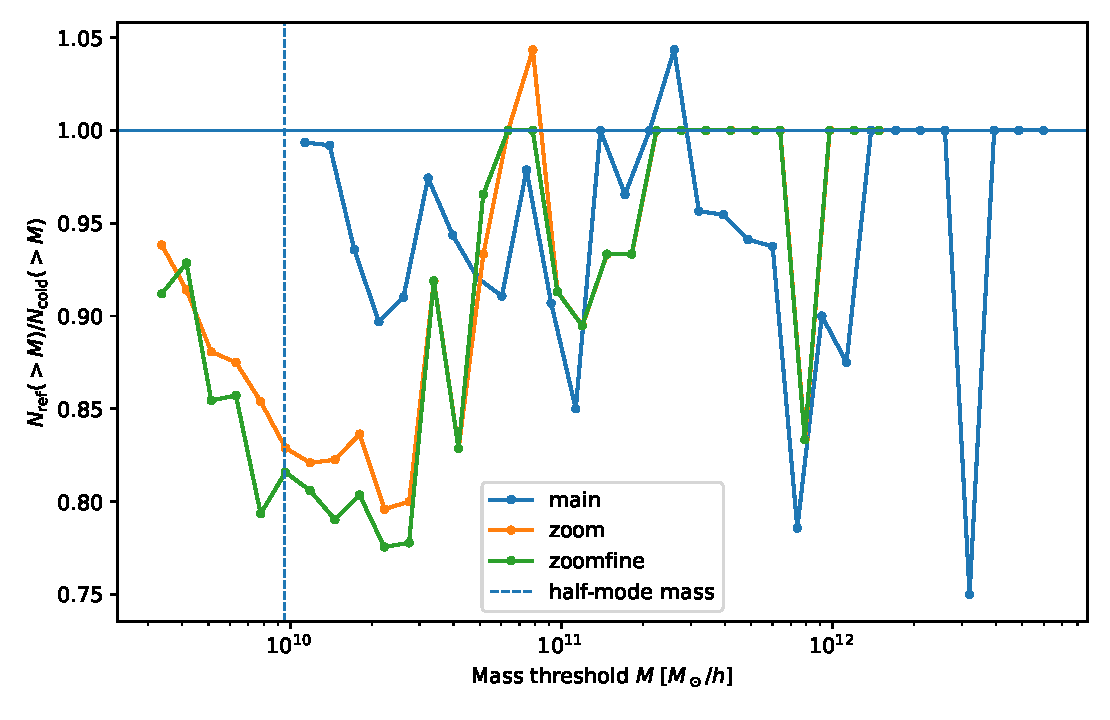
\includegraphics[width=0.86\linewidth]{figures/halo/01_cumulative_halo_abundance.pdf}
\caption{Paired cumulative halo abundance.  The vertical line is the linear half-mode mass.  Low-count high-mass points are shown for completeness but carry large finite-volume uncertainty.}
\label{fig:cumulative-halo-abundance}
\end{figure}

\section{Matched halo structure}

The zoom run yields $93$ mutual matches, of which $66$ pass the robust cut.  Their median ratios are
\begin{equation}
\boxed{
\begin{aligned}
\operatorname{med}\frac{M_{\rm ref}}{M_{\rm cold}}&=0.83371,\\
\operatorname{med}\frac{V_{\max,\rm ref}}{V_{\max,\rm cold}}&=0.94438,\\
\operatorname{med}\frac{r_{1/2,\rm ref}}{r_{1/2,\rm cold}}&=0.95535,\\
\operatorname{med}\frac{\sigma_{1\rm d,ref}}{\sigma_{1\rm d,cold}}&=0.96729.
\end{aligned}}
\label{eq:matched-halo-medians}
\end{equation}
The time-control medians are $0.82155$, $0.94496$, $0.95230$, and $0.96611$, respectively.  The median Jaccard overlap is $0.663$ in the zoom run and $0.675$ in the time control.

These results indicate that, for corresponding Lagrangian structures, refinement halos typically retain less FoF mass and a lower maximum circular-speed proxy.  The radius shift is smaller than the mass shift.  The PM force scale is too coarse for a precision concentration statement.

\begin{figure}[htbp]
\centering
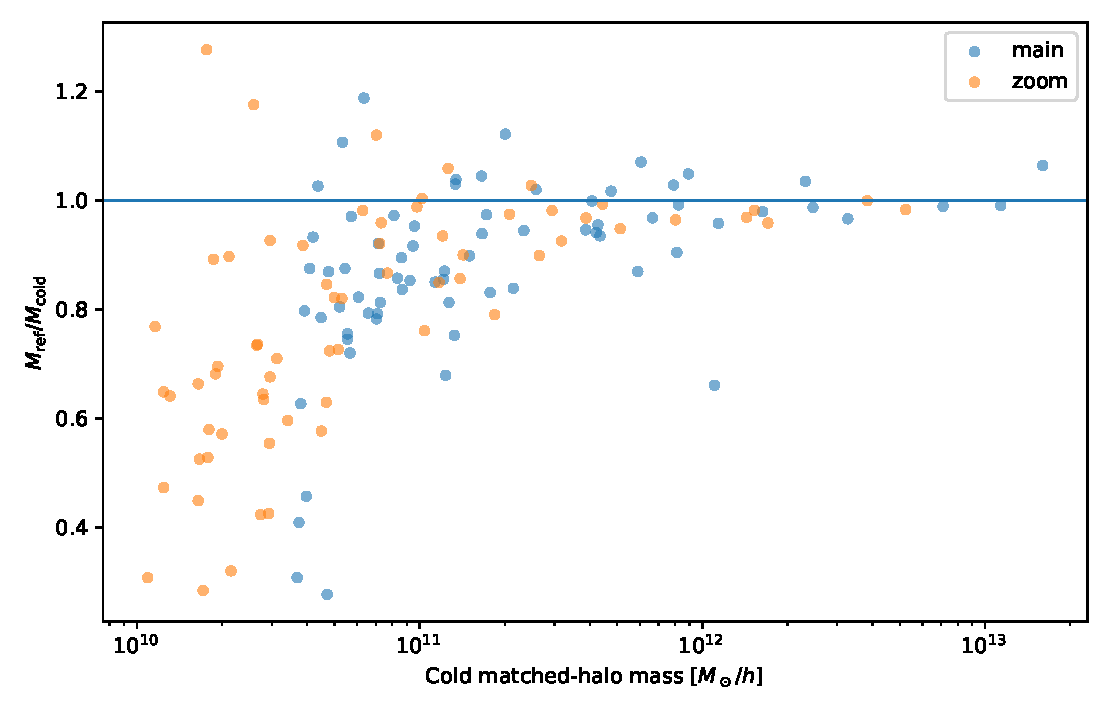
\includegraphics[width=0.84\linewidth]{figures/halo/02_matched_mass_ratios.pdf}
\caption{Particle-overlap matched halo masses.  Paired phases permit object-by-object comparison rather than comparison of two unrelated catalogues.}
\label{fig:matched-mass-ratios}
\end{figure}

\begin{figure}[htbp]
\centering
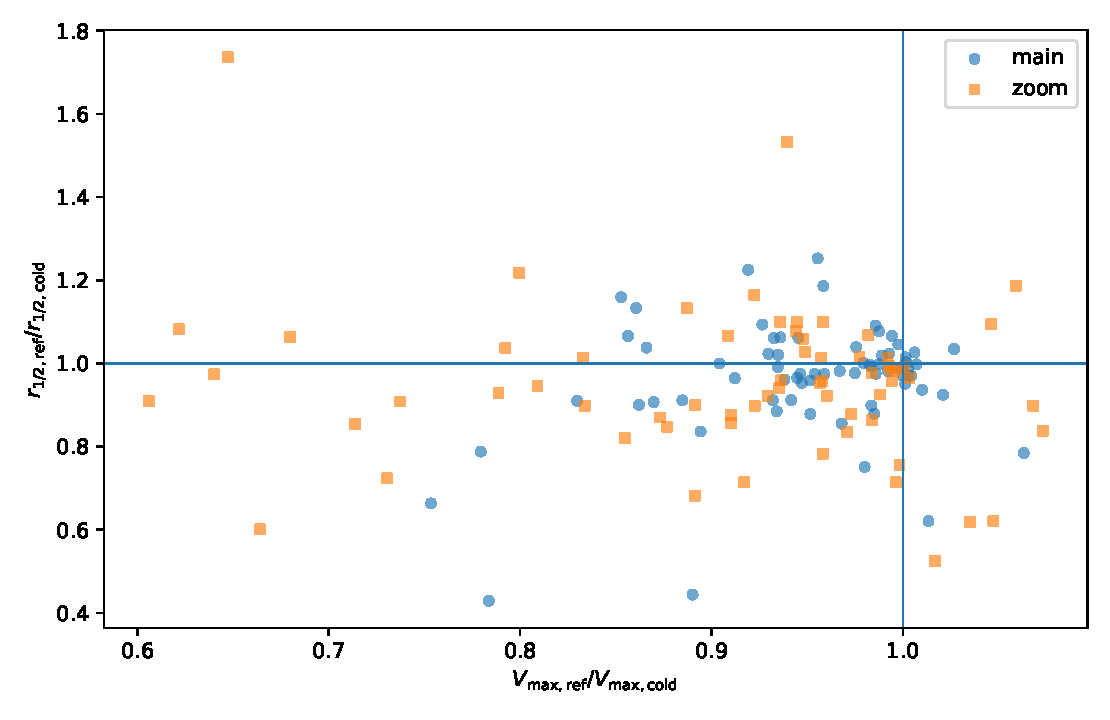
\includegraphics[width=0.78\linewidth]{figures/halo/03_matched_structure_ratios.pdf}
\caption{Matched maximum-speed and half-mass-radius proxies.  The scatter is physical, finite-resolution, and halo-finder dependent.}
\label{fig:matched-structure-ratios}
\end{figure}

\section{Assembly delay}

For the robust zoom matches, the population medians of the assembly proxy are
\begin{equation}
 \operatorname{med} f_{1/2}^{\rm cold}=0.42308,
 \qquad
 \operatorname{med} f_{1/2}^{\rm ref}=0.34836.
\label{eq:formation-population-medians}
\end{equation}
The median of the matched per-halo ratio is
\begin{equation}
\boxed{
 \operatorname{med}
 \left(
 \frac{f_{1/2}^{\rm ref}}{f_{1/2}^{\rm cold}}
 \right)
 =0.90426.}
\label{eq:formation-ratio}
\end{equation}
The $360$-step control gives $0.91483$.  Thus corresponding refinement halos have, on average, a smaller fraction of their final particles assembled into one FoF progenitor at $a=0.5$.  This is evidence for delayed assembly in the pilot, not a calibrated formation-redshift law.

\begin{figure}[htbp]
\centering
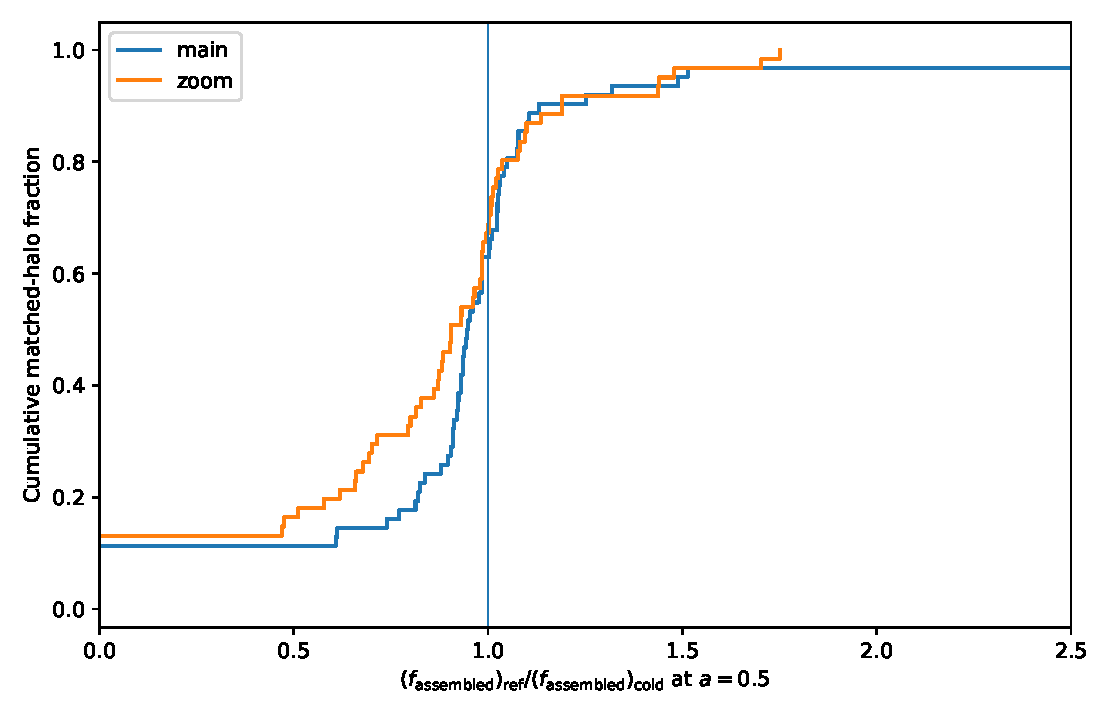
\includegraphics[width=0.80\linewidth]{figures/halo/04_formation_delay_cdf.pdf}
\caption{Cumulative distribution of the matched one-step assembly ratio.  Values below unity indicate later assembly in the refinement realization.  The horizontal range is truncated at $2.5$ so that a few small-denominator outliers do not obscure the central distribution.}
\label{fig:formation-delay}
\end{figure}

\section{Convergence and controls}

Across thresholds with at least five cold halos, the maximum difference between the $260$- and $360$-step cumulative abundance ratios is
\begin{equation}
 \epsilon_{\Delta t}=0.06042.
\label{eq:halo-time-control}
\end{equation}
At the physically central half-mode threshold the difference is only
\begin{equation}
 |0.82980-0.81507|=0.01473.
\label{eq:halo-half-mode-time-control}
\end{equation}
The maximum main-to-zoom paired-ratio discrepancy in their overlapping, count-controlled mass range is
\begin{equation}
 \epsilon_{\rm box}=0.17093.
\label{eq:halo-box-control}
\end{equation}
This includes different random phases and finite-volume effects and is not a strict spatial-convergence error.

\begin{figure}[htbp]
\centering
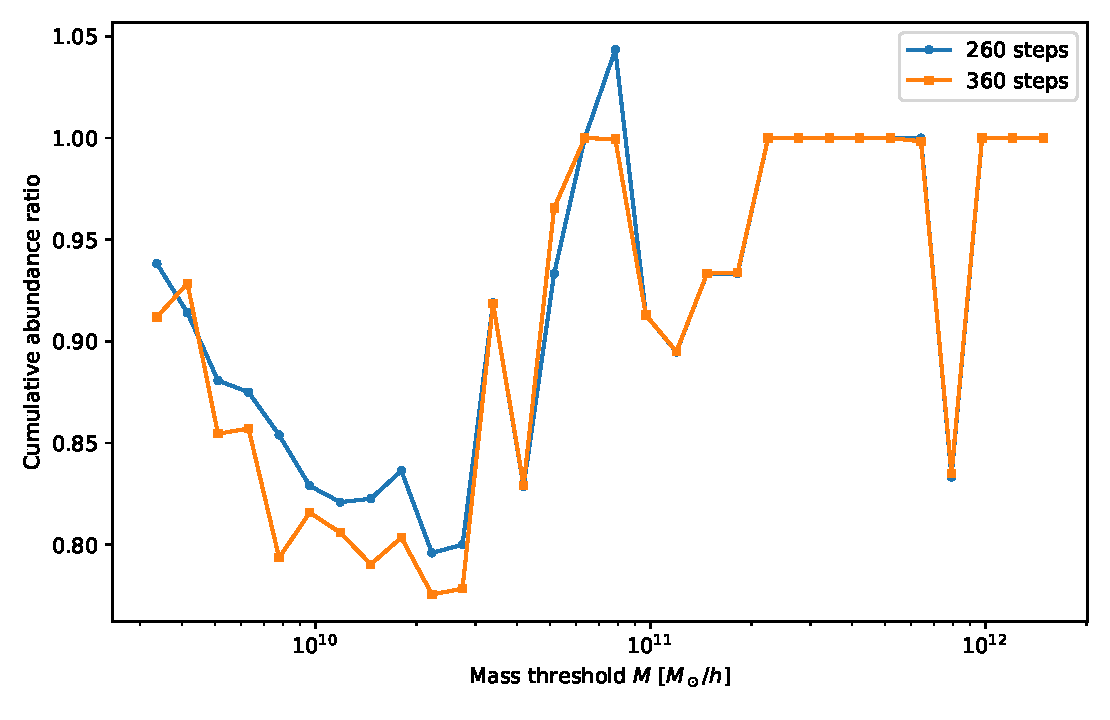
\includegraphics[width=0.82\linewidth]{figures/halo/05_time_step_control.pdf}
\caption{Time-step control in the $8\,h^{-1}\,\mathrm{Mpc}$ box.  Discrete halo counts make the curve non-smooth.}
\label{fig:halo-time-control}
\end{figure}

The deterministic audit records
\begin{equation}
\boxed{19\ \mathrm{PASS},\qquad0\ \mathrm{FAIL}.}
\label{eq:halo-audit-count}
\end{equation}
It checks nonempty catalogues, mass partition bounds, mutual matches, time and box controls, half-mode suppression, finite structural and formation ratios, label invariance, and the large-scale mass--dipole protection theorem.

\section{Physical interpretation}

The pilot sharpens the nonlinear prediction of the scale-covariant refinement dark sector:
\begin{equation}
\boxed{
\begin{aligned}
\text{large halos:}&\quad \text{approximately cold-like abundance and structure},\\
\text{near-cutoff halos:}&\quad \text{reduced abundance, mass, and }V_{\max},\\
\text{assembly:}&\quad \text{a later largest-progenitor fraction},\\
\text{two-point power:}&\quad \text{substantial nonlinear regeneration remains possible}.
\end{aligned}}
\label{eq:halo-physical-pattern}
\end{equation}
This supports the conclusion that low-mass halo counts and assembly histories retain more memory of the primordial refinement cutoff than the final nonlinear matter power alone.

\section{Claim boundary and unresolved requirements}

The calculation does not yet provide:
\begin{itemize}
\item a large-volume, high-dynamic-range halo mass function;
\item force- and particle-resolution convergence at fixed volume;
\item subhalo catalogues or converged internal density profiles;
\item baryonic hydrodynamics, cooling, star formation, or feedback;
\item a survey selection function or observational likelihood;
\item a first-principles value of the refinement mass and production scales.
\end{itemize}

A production-level nonlinear falsification test requires
\begin{equation}
\boxed{
\begin{gathered}
\text{large-volume and zoom-refined halo catalogues}\\
+\text{baryonic response envelopes}\\
+\text{frozen-parameter lensing and satellite observables}\\
\Longrightarrow
\text{first joint nonlinear falsification test}.
\end{gathered}}
\label{eq:halo-open-requirements}
\end{equation}

\chapter[Baryonic Response and Nonlinear Falsification]{Baryonic Response Envelopes and Frozen-Parameter Nonlinear Falsification}
\label{ch:baryonic-response-falsification}

\section{Scope and objective}

The preceding chapters establish a fixed collisionless transfer function, a coupled Einstein--Boltzmann calculation, nonlinear power regeneration, explicit paired halo catalogues, particle-overlap matching, and one-step assembly proxies.  The unresolved interface addressed here is baryonic.  A collisionless halo deficit does not immediately imply a galaxy or satellite deficit because gas retention, photoheating, cooling, star formation, and feedback can amplify or mask the gravitational difference.

This chapter does not pretend to replace hydrodynamics.  It constructs a controlled \emph{response envelope}: the same monotone baryonic map is applied to the cold and refinement halo catalogues over a declared nuisance-parameter family.  This isolates which signatures survive broad common baryonic uncertainty and which remain under-resolved.

The fixed input is the paired $8\,h^{-1}{\rm Mpc}$ halo calculation and its independent $260$- versus $360$-step control.  No refinement parameter is retuned.  The principal result is
\begin{equation}
\boxed{
\begin{gathered}
\text{global baryonic mass budget nearly cold-like},\\
\text{luminous halo count suppressed by roughly }8\%-18\%,\\
\text{near-cutoff matched stellar proxy suppressed much more strongly},\\
\text{CMB and nonlinear lensing remain nearly cold-like},\\
\text{host-centric satellite proxy not yet numerically converged}.
\end{gathered}}
\label{eq:brf-principal-result}
\end{equation}

\section{Declared baryonic response family}

Let $M$ and $V$ denote the halo mass and maximum-circular-speed proxy.  The luminous occupation probability is
\begin{equation}
P_{\rm lum}(V;V_{50},s)
=
\left[1+\exp\left(-\frac{\log(V/V_{50})}{s}\right)\right]^{-1}.
\label{eq:brf-occupation}
\end{equation}
The scan uses
\begin{equation}
V_{50}\in\{15,20,25,30,35,40,50\}\ {\rm km\,s^{-1}},
\qquad
s\in\{0.15,0.25,0.40,0.60\}.
\label{eq:brf-occupation-grid}
\end{equation}

A gas-retention envelope is
\begin{equation}
M_{\rm gas}(M,V)
\propto
\frac{M}{1+(V_{\rm evap}/V)^\eta},
\label{eq:brf-gas-response}
\end{equation}
and a stellar-response proxy is
\begin{equation}
M_\star(M,V)
\propto
\frac{M}{1+(V_{\rm evap}/V)^\eta}
\frac{(V/V_\star)^\alpha}{1+(V/V_\star)^\alpha}.
\label{eq:brf-stellar-response}
\end{equation}
The common response parameters are scanned over
\begin{equation}
\begin{aligned}
V_{\rm evap}&\in\{15,20,25,30,40\}\ {\rm km\,s^{-1}},\\
\eta&\in\{2,3,4,6\},\\
V_\star&\in\{25,40,60,80\}\ {\rm km\,s^{-1}},\\
\alpha&\in\{1,2,3\}.
\end{aligned}
\label{eq:brf-response-grid}
\end{equation}
The cosmic baryon fraction and the maximum conversion efficiency cancel from all refinement-to-cold ratios.  These maps are deliberately broad nuisance envelopes.  They are not calibrated sub-grid physics.

\section{Monotone occupation theorem}

\begin{theorem}[Cumulative ordering implies luminous-count ordering]
Let $\mu_C$ and $\mu_R$ be cold and refinement halo measures on a scalar halo property $x$, with cumulative counts
\[
N_X(>x)=\mu_X((x,\infty)),\qquad X\in\{C,R\}.
\]
Assume
\[
N_R(>x)\le N_C(>x)
\]
for every $x$.  Then every bounded nondecreasing occupation function $p(x)\ge0$ satisfies
\begin{equation}
\int p\,d\mu_R\le\int p\,d\mu_C.
\label{eq:brf-monotone-ordering}
\end{equation}
\end{theorem}

\begin{proof}
For an absolutely continuous $p$ with $p(0)=0$, Stieltjes integration by parts gives
\[
\int p(x)\,d\mu_X(x)
=
\int_0^\infty p'(x)N_X(>x)\,dx.
\]
Since $p'\ge0$, cumulative ordering gives the result.  General bounded nondecreasing $p$ follows by monotone approximation.
\end{proof}

The $360$-step catalogue obeys cumulative refinement-to-cold abundance no greater than one at every archived mass threshold.  The theorem therefore gives a sign-definite luminous-count suppression for any common monotone occupation applied to that time-control catalogue.  The $260$-step catalogue has one isolated high-mass bin slightly above unity because of finite object counts, but every occupation model in the declared scan still yields a total ratio below one.

\section{Global luminous and baryonic envelopes}

The expected luminous count is
\begin{equation}
N_{\rm lum}=\sum_H P_{\rm lum}(V_{\max,H}).
\label{eq:brf-expected-luminous-count}
\end{equation}
The complete occupation scan gives
\begin{center}
\begin{tabular}{lccc}
\toprule
run & minimum & median & maximum\\
\midrule
$260$-step zoom & $0.841250$ & $0.894665$ & $0.920903$\\
$360$-step control & $0.819753$ & $0.874244$ & $0.915456$\\
\bottomrule
\end{tabular}
\end{center}
Thus the global expected luminous-halo count is lower by approximately $8\%-18\%$ throughout the declared occupation family.

\begin{figure}[htbp]
\centering
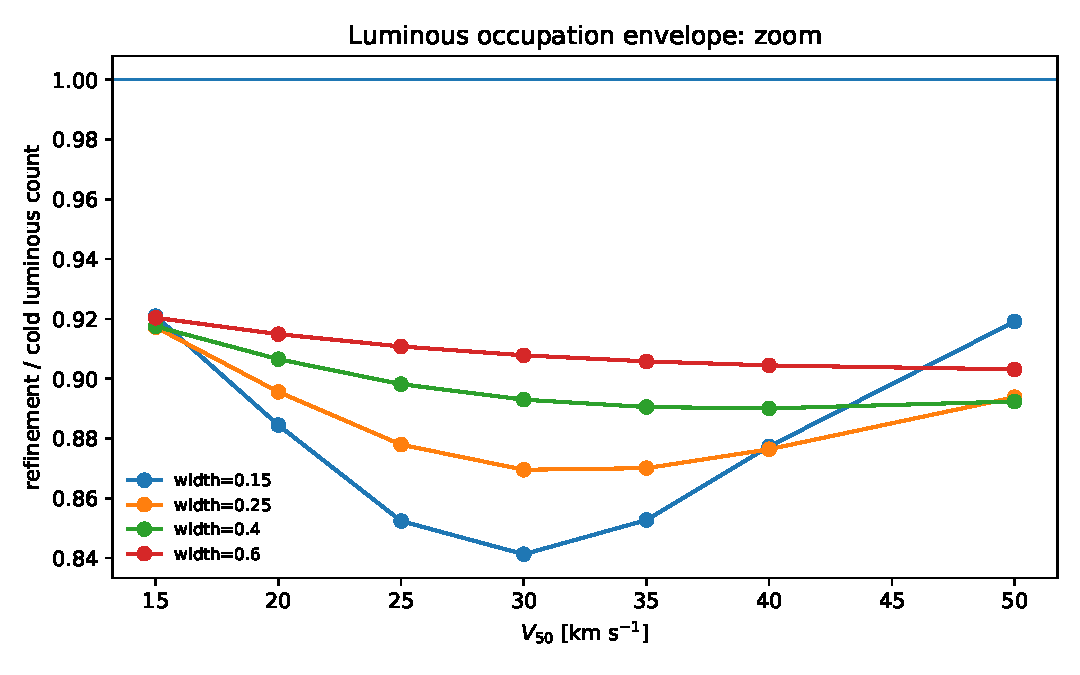
\includegraphics[width=.80\linewidth]{figures/brf/luminous_occupation_zoom.pdf}
\caption{Global luminous-count ratio in the $260$-step zoom catalogue.  Every declared monotone occupation model remains below unity.}
\label{fig:brf-luminous-zoom}
\end{figure}

The integrated baryonic mass budget is much less sensitive because the most massive halos dominate the sum:
\begin{center}
\begin{tabular}{lccc}
\toprule
observable & minimum & median & maximum\\
\midrule
zoom total gas ratio & $0.955236$ & $0.958096$ & $0.963734$\\
zoom total stellar proxy & $0.958112$ & $0.964322$ & $0.968384$\\
time-control total gas ratio & $0.958151$ & $0.961867$ & $0.969067$\\
time-control total stellar proxy & $0.961980$ & $0.970086$ & $0.975786$\\
\bottomrule
\end{tabular}
\end{center}
The model therefore does not predict a comparably large deficit in the total low-redshift baryonic mass budget.  Its sharper signature lies in the distribution of that mass among low-mass objects.

\section{Matched baryonic amplification near the cutoff}

For one matched halo pair, write
\[
R_M=\frac{M_R}{M_C},
\qquad
R_V=\frac{V_R}{V_C}.
\]
For any response of the form
\[
B(M,V)=M f(V)g(V)
\]
with $f$ and $g$ nondecreasing,
\begin{equation}
\frac{B_R}{B_C}
=
R_M\frac{f(R_VV_C)}{f(V_C)}\frac{g(R_VV_C)}{g(V_C)}.
\label{eq:brf-matched-response-ratio}
\end{equation}
Hence
\begin{equation}
R_M\le1,
\quad R_V\le1
\quad\Longrightarrow\quad
\frac{B_R}{B_C}\le R_M\le1.
\label{eq:brf-baryonic-amplification-theorem}
\end{equation}
In the robust zoom sample, $80.303\%$ of matched pairs satisfy both $R_M<1$ and $R_V<1$.

The response scan gives the following median matched stellar-proxy envelopes:
\begin{center}
\small
\begin{tabular}{lccc|ccc}
\toprule
&\multicolumn{3}{c}{260-step zoom}&\multicolumn{3}{c}{360-step control}\\
maximum cold mass & min & median & max & min & median & max\\
\midrule
$3\times10^{10}\,h^{-1}M_\odot$ & $0.1411$ & $0.3962$ & $0.5668$ & $0.1337$ & $0.3881$ & $0.5780$\\
$10^{11}\,h^{-1}M_\odot$ & $0.3371$ & $0.5836$ & $0.6430$ & $0.3128$ & $0.5752$ & $0.6392$\\
$3\times10^{11}\,h^{-1}M_\odot$ & $0.6266$ & $0.7130$ & $0.7468$ & $0.5941$ & $0.6997$ & $0.7424$\\
$10^{12}\,h^{-1}M_\odot$ & $0.7157$ & $0.7627$ & $0.7827$ & $0.7092$ & $0.7457$ & $0.7817$\\
\bottomrule
\end{tabular}
\end{center}

\begin{figure}[htbp]
\centering
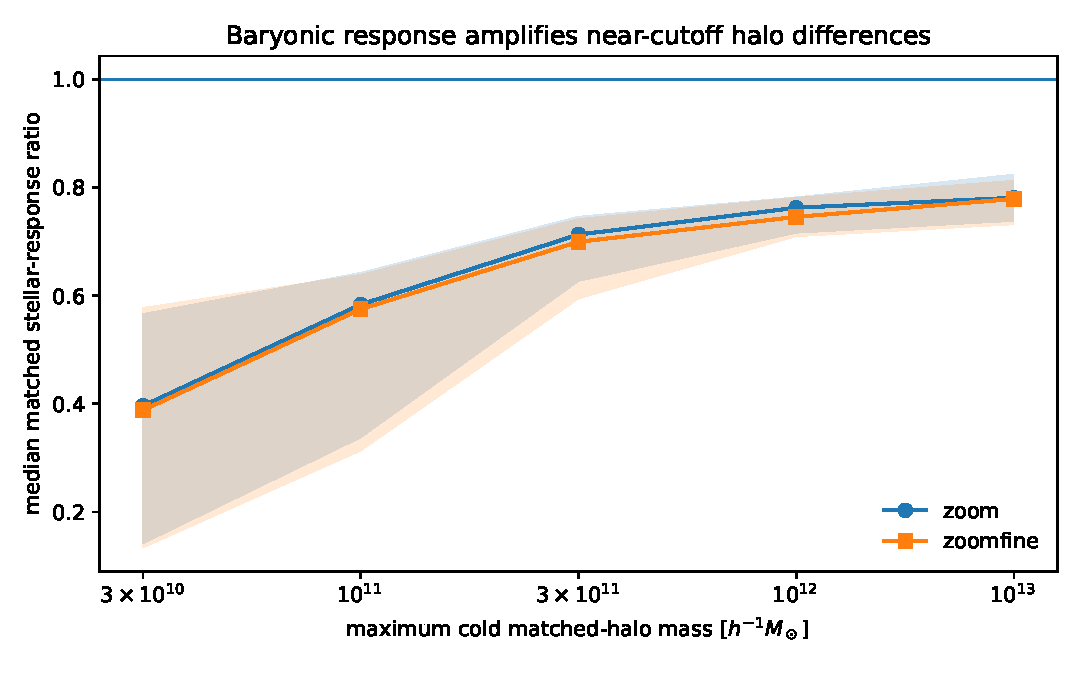
\includegraphics[width=.82\linewidth]{figures/brf/matched_stellar_response_envelope.pdf}
\caption{The same baryonic response applied to matched halos amplifies the gravitational difference near the cutoff.  Shaded regions show the full declared response envelope.}
\label{fig:brf-matched-stellar}
\end{figure}

For matched halos below $3\times10^{10}\,h^{-1}M_\odot$, the median stellar proxy is only about $0.39$ of the cold value.  The time-control discrepancy in that median is $0.00805$.  The near-cutoff conclusion is therefore materially stronger and more stable than the small difference in the total stellar budget.

\section{Structural and lensing proxies}

The matched catalogue directly supplies mass, half-mass radius, $V_{\max}$, and velocity-dispersion proxies.  Define
\begin{equation}
\Sigma_{1/2}^{\rm proxy}
:=
\frac{M}{2\pi r_{1/2}^2},
\qquad
S_{\rm dyn}^{\rm proxy}
:=
\frac{V_{\max}^2}{r_{1/2}}.
\label{eq:brf-structural-proxies}
\end{equation}
Their refinement-to-cold ratios are
\begin{equation}
R_{\Sigma}
=
\frac{R_M}{R_{r_{1/2}}^2},
\qquad
R_{\rm dyn}
=
\frac{R_V^2}{R_{r_{1/2}}}.
\label{eq:brf-structural-ratios}
\end{equation}
For the robust zoom sample,
\begin{equation}
\boxed{
\operatorname{median}R_{\Sigma}=0.925269,
\qquad
\operatorname{median}R_{\rm dyn}=0.933888.
}
\label{eq:brf-structural-medians}
\end{equation}
The fractions below unity are $0.681818$ and $0.696970$, respectively.

\begin{figure}[htbp]
\centering
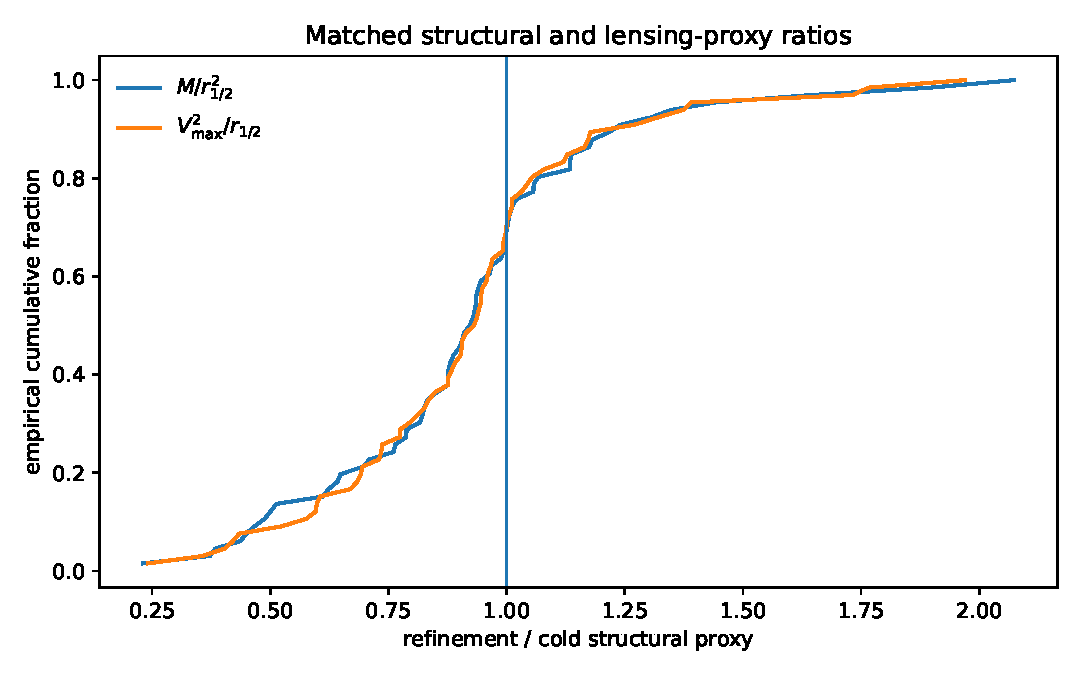
\includegraphics[width=.80\linewidth]{figures/brf/matched_surface_density_cdf.pdf}
\caption{Empirical cumulative distributions of the matched half-mass and dynamical surface-density proxies.}
\label{fig:brf-surface-cdf}
\end{figure}

These are not precision galaxy--galaxy lensing predictions because the FoF mass is not a calibrated spherical-overdensity mass and no resolved baryonic profile is present.  They do show that the matched near-cutoff structures tend to have lower projected and dynamical density scales before any branch-dependent baryonic compensation is introduced.

\section{Frozen-parameter cross-observable signature}

For any observable ratio $R<1$, define the branch-dependent baryonic enhancement required to restore unity,
\begin{equation}
\Delta_B^{\rm erase}:=\frac1R-1.
\label{eq:brf-erasure-boost}
\end{equation}
This does not assert whether such a boost is astrophysically plausible.  It states the exact differential response required to erase the gravitational prediction.

\begin{center}
\small
\begin{tabular}{p{.47\linewidth}rr}
\toprule
observable & $R$ & required boost\\
\midrule
CMB lensing at $L=3000$ & $0.995081$ & $0.49\%$\\
nonlinear galaxy lensing, $z_s=0.5$, $\ell=5000$ & $0.985017$ & $1.52\%$\\
global luminous count, zoom median & $0.894665$ & $11.77\%$\\
global luminous count, time control & $0.874244$ & $14.38\%$\\
matched stellar proxy, $M\le3\times10^{10}\,h^{-1}M_\odot$ & $0.396164$ & $152.42\%$\\
matched half-mass surface-density proxy & $0.925269$ & $8.08\%$\\
atomic-cooling collapsed fraction at $z=7.4$ & $0.342283$ & $192.16\%$\\
\bottomrule
\end{tabular}
\end{center}

\begin{figure}[htbp]
\centering
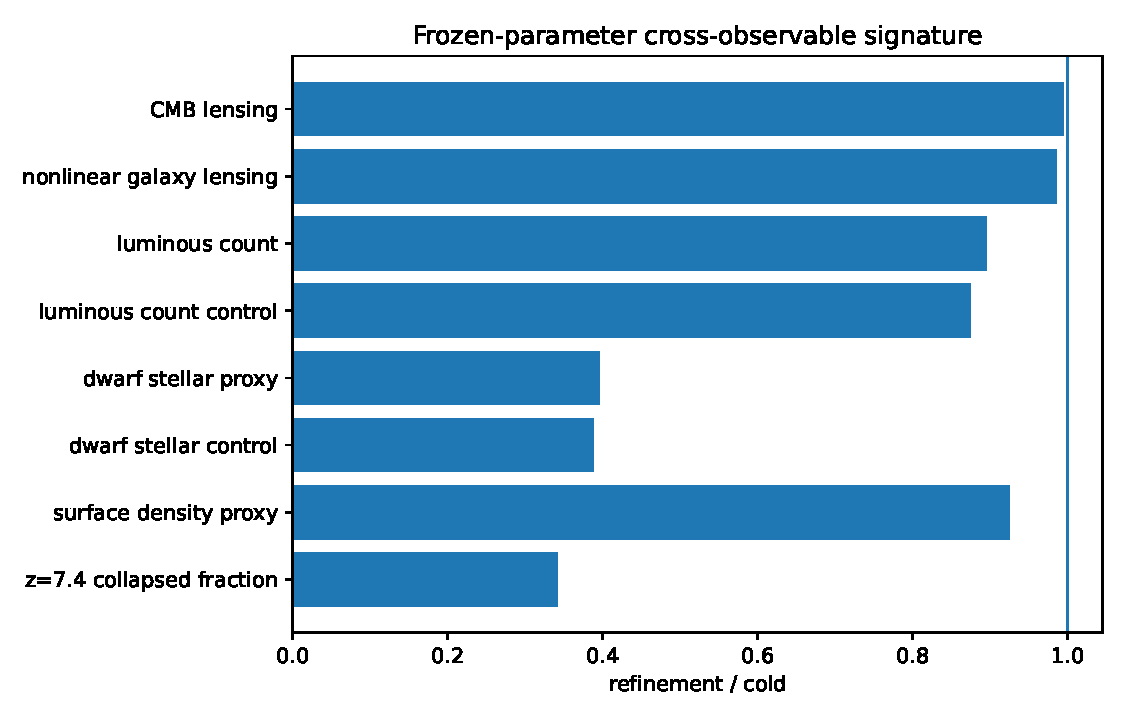
\includegraphics[width=.84\linewidth]{figures/brf/joint_falsification_signature.pdf}
\caption{One frozen dark-sector parameter set predicts nearly cold CMB and nonlinear lensing together with much stronger dwarf-scale and high-redshift suppression.}
\label{fig:brf-joint-signature}
\end{figure}

The cross-observable pattern is therefore
\begin{equation}
\boxed{
\text{CMB and bulk lensing nearly cold}
\quad+
\text{dwarf luminosity and early collapse strongly suppressed}.
}
\label{eq:brf-linked-signature}
\end{equation}
A data set showing the opposite combination would reject this branch more sharply than any one observable alone.

\section{Satellite-neighborhood negative control}

A host-centric count was also constructed around the five most massive matched hosts.  Every neighboring FoF halo within radius $R$ was weighted by the same occupation family.  This is only a satellite-candidate proxy because the FoF catalogue does not resolve subhalos inside the host component.

\begin{center}
\begin{tabular}{lcccc}
\toprule
run & $R\,[h^{-1}{\rm Mpc}]$ & minimum & median & maximum\\
\midrule
zoom & $0.5$ & $0.825$ & $1.283$ & $1.344$\\
zoom & $1.0$ & $0.985$ & $1.156$ & $1.223$\\
zoom & $1.5$ & $0.934$ & $1.052$ & $1.112$\\
time control & $0.5$ & $0.403$ & $1.039$ & $1.102$\\
time control & $1.0$ & $0.915$ & $1.009$ & $1.070$\\
time control & $1.5$ & $0.900$ & $0.976$ & $1.020$\\
\bottomrule
\end{tabular}
\end{center}

\begin{figure}[htbp]
\centering
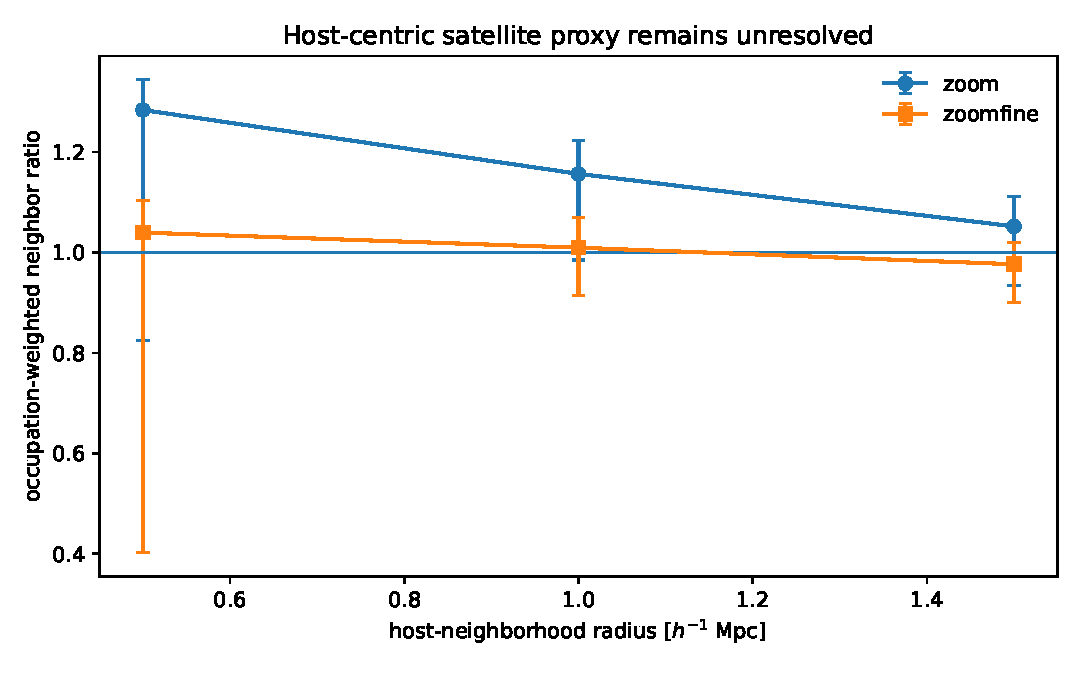
\includegraphics[width=.80\linewidth]{figures/brf/host_neighborhood_control.pdf}
\caption{The host-neighborhood proxy changes materially under the time-step control and crosses unity across the baryonic envelope.  It is not yet a stable satellite prediction.}
\label{fig:brf-host-control}
\end{figure}

This negative control is important.  The global luminous count and matched dwarf response are stable, but a true satellite prediction requires a subhalo finder, higher force resolution, host zooms, and disruption tracking.

\section{Verification ledger}

The deterministic audit records
\begin{equation}
\boxed{20\ {\rm PASS},\qquad0\ {\rm FAIL}.}
\label{eq:brf-pass-count}
\end{equation}
Selected controls are
\begin{center}
\begin{tabular}{lr}
\toprule
control & residual or value\\
\midrule
maximum global occupation ratio & $0.920903$\\
zoom/time-control occupation-median difference & $0.020421$\\
near-cutoff response-median difference & $0.008050$\\
median half-mass surface-density ratio & $0.925269$\\
robust matches with both $M_R<M_C$ and $V_R<V_C$ & $0.803030$\\
CMB-lensing ratio at $L=3000$ & $0.995081$\\
nonlinear galaxy-lensing ratio at $\ell=5000$ & $0.985017$\\
reionization efficiency penalty at $z=7.4$ & $2.921558$\\
\bottomrule
\end{tabular}
\end{center}
The input hashes, full response scans, structural tables, and check records are included in the reproducibility package.

\section{Claim boundary}

This chapter establishes:
\begin{itemize}
\item an exact monotone occupation-ordering theorem;
\item a frozen common-response envelope for luminous counts, gas, and stellar proxies;
\item a matched-halo theorem showing how velocity suppression amplifies baryonic suppression;
\item controlled near-cutoff stellar-response and structural-proxy ratios;
\item a cross-observable erasure threshold with no dark-sector retuning;
\item a negative control showing that the present host-centric satellite proxy is not converged.
\end{itemize}

It does not establish:
\begin{itemize}
\item hydrodynamic cooling, star formation, or feedback from first principles;
\item resolved subhalo catalogues or disruption histories;
\item calibrated galaxy luminosities or stellar-mass functions;
\item survey selection, covariance, foregrounds, or a likelihood;
\item microscopic values of $a_\star$, $\Lambda$, $\gamma$, or the physical mass scale;
\item radiative stability, independent reproduction, or literature priority.
\end{itemize}

\chapter[Cooling, Feedback, and Ionizing Sources]{One Zone Cooling, Feedback, and Ionizing Source Closure}
\label{ch:cooling-feedback-reionization}

% Generated by Cooling_Feedback_Reionization_Verification.py
\newcommand{\CFRAtomicVelocity}{16.727527}
\newcommand{\CFRPairZoom}{53}
\newcommand{\CFRPairControl}{52}
\newcommand{\CFRMassResidual}{1.807e-15}
\newcommand{\CFRZoomTotalStarMin}{0.960484}
\newcommand{\CFRZoomTotalStarMedian}{0.962352}
\newcommand{\CFRZoomTotalStarMax}{0.966885}
\newcommand{\CFRControlTotalStarMin}{0.960151}
\newcommand{\CFRControlTotalStarMedian}{0.962225}
\newcommand{\CFRControlTotalStarMax}{0.966525}
\newcommand{\CFRZoomDwarfStarMin}{0.461458}
\newcommand{\CFRZoomDwarfStarMedian}{0.549254}
\newcommand{\CFRZoomDwarfStarMax}{0.606955}
\newcommand{\CFRControlDwarfStarMin}{0.482247}
\newcommand{\CFRControlDwarfStarMedian}{0.597254}
\newcommand{\CFRControlDwarfStarMax}{0.652880}
\newcommand{\CFRZoomDwarfSFRMin}{0.441567}
\newcommand{\CFRZoomDwarfSFRMedian}{0.517358}
\newcommand{\CFRZoomDwarfSFRMax}{0.616550}
\newcommand{\CFRControlDwarfSFRMin}{0.432337}
\newcommand{\CFRControlDwarfSFRMedian}{0.508604}
\newcommand{\CFRControlDwarfSFRMax}{0.619121}
\newcommand{\CFRIonMin}{0.433826}
\newcommand{\CFRIonMedian}{0.520843}
\newcommand{\CFRIonMax}{0.639050}
\newcommand{\CFRBoostMin}{1.564824}
\newcommand{\CFRBoostMedian}{1.919965}
\newcommand{\CFRBoostMax}{2.305070}
\newcommand{\CFRPriorPenalty}{2.921558}
\newcommand{\CFROrderedZoom}{17}
\newcommand{\CFROrderedControl}{18}
\newcommand{\CFRMaxOrderedStar}{0.966845}
\newcommand{\CFRPass}{20}
\newcommand{\CFRFail}{0}


\section{Scope and objective}

The scale covariant refinement model now has a fixed collisionless transfer function, primary and late time observable calculations, nonlinear particle evolution, paired halo catalogues, and broad baryonic response envelopes.  The unresolved physical interface is the conversion of halo growth into gas, stars, outflows, and ionizing sources.

This chapter introduces a mass conserving one zone regulator.  It is applied to the cold and refinement halo histories with exactly the same cooling and feedback parameters.  No dark sector parameter is retuned.  The calculation has two purposes:
\begin{enumerate}
\item replace the previous static baryonic response map by a time dependent gas budget with explicit inflow, cooling, star formation, recycling, and outflow;
\item propagate the same response law into the high redshift halo mass functions and measure the remaining ionizing emissivity burden.
\end{enumerate}

The principal result is
\begin{equation}
\boxed{
\begin{aligned}
\text{matched total stellar budget} &\simeq 0.96\times\text{cold},\\
\text{near cutoff stellar mass and SFR} &\simeq 0.4\text{--}0.65\times\text{cold},\\
\text{ionizing source at }z=7.4 &\simeq 0.43\text{--}0.64\times\text{cold},\\
\text{required source enhancement} &\simeq 1.56\text{--}2.31.
\end{aligned}}
\label{eq:cfr-principal-result}
\end{equation}

The calculation is a controlled one zone closure.  It is not a hydrodynamic simulation and does not resolve a multiphase interstellar medium.

\section{Virial temperature and the atomic cooling scale}

For mean molecular weight $\mu$, define the virial temperature from the halo speed $V$ by
\begin{equation}
T_{\rm vir}(V)
=
\frac{\mu m_pV^2}{2k_B}.
\label{eq:cfr-virial-temperature}
\end{equation}
With $\mu=0.59$,
\begin{equation}
T_{\rm vir}
=
35.74\ {\rm K}
\left(\frac{V}{1\ {\rm km\,s^{-1}}}\right)^2.
\label{eq:cfr-temperature-speed}
\end{equation}
The declared atomic threshold $T_{\rm atom}=10^4\ {\rm K}$ therefore corresponds to
\begin{equation}
\boxed{
V_{\rm atom}=\CFRAtomicVelocity\ {\rm km\,s^{-1}}.
}
\label{eq:cfr-atomic-speed}
\end{equation}

The smooth atomic cooling gate is
\begin{equation}
C_{\rm atom}(V)
=
\left[
1+
\left(
\frac{T_{\rm atom}}{T_{\rm vir}(V)}
\right)^{n_{\rm atom}}
\right]^{-1}.
\label{eq:cfr-atomic-gate}
\end{equation}
After the calibrated reionization midpoint, the photoheating gate is
\begin{equation}
C_{\rm ph}(V)
=
\left[
1+
\left(
\frac{V_{\rm ph}}{V}
\right)^4
\right]^{-1}.
\label{eq:cfr-photo-gate}
\end{equation}
Before reionization, $C_{\rm ph}=1$.

Energy driven outflow is represented by the mass loading
\begin{equation}
\eta_w(V)
=
\left(
\frac{V_{\rm fb}}{V}
\right)^\beta.
\label{eq:cfr-mass-loading}
\end{equation}
This response is common to both dark matter branches.

\section{Mass conserving gas regulator}

Let $M_h(a)$ be one halo growth history.  Define gas, long lived stars, and expelled material by
\begin{equation}
M_g(a),\qquad M_\star(a),\qquad M_{\rm out}(a).
\end{equation}
Use the stellar return fraction $R$ and a dynamical time
\begin{equation}
t_{\rm dyn}=\xi H^{-1},
\qquad
\xi=0.1.
\label{eq:cfr-dynamical-time}
\end{equation}
The star formation rate before recycling is
\begin{equation}
\psi
=
\frac{\epsilon_{\rm ff}}{t_{\rm dyn}}
C_{\rm atom}C_{\rm ph}M_g.
\label{eq:cfr-star-formation-rate}
\end{equation}
Using $a$ as the independent variable, the regulator is
\begin{align}
\frac{dM_g}{da}
&=
f_b\frac{dM_h}{da}
-
\frac{\epsilon_{\rm ff}C_{\rm atom}C_{\rm ph}}{\xi a}
(1-R+\eta_w)M_g,
\label{eq:cfr-gas-equation}
\\
\frac{dM_\star}{da}
&=
\frac{\epsilon_{\rm ff}C_{\rm atom}C_{\rm ph}}{\xi a}
(1-R)M_g,
\label{eq:cfr-star-equation}
\\
\frac{dM_{\rm out}}{da}
&=
\frac{\epsilon_{\rm ff}C_{\rm atom}C_{\rm ph}}{\xi a}
\eta_wM_g.
\label{eq:cfr-outflow-equation}
\end{align}

\begin{theorem}[Exact baryonic mass budget]
For every nondecreasing halo history,
\begin{equation}
\frac{d}{da}
\left(
M_g+M_\star+M_{\rm out}-f_bM_h
\right)
=0.
\label{eq:cfr-budget-derivative}
\end{equation}
If the initial state satisfies $M_g=f_bM_h$ and $M_\star=M_{\rm out}=0$, then
\begin{equation}
\boxed{
M_g(a)+M_\star(a)+M_{\rm out}(a)=f_bM_h(a)
}
\label{eq:cfr-exact-budget}
\end{equation}
for all later $a$.
\end{theorem}

\begin{proof}
Add equations \eqref{eq:cfr-gas-equation} through \eqref{eq:cfr-outflow-equation}.  The cooling, star formation, recycling, and outflow terms cancel exactly.  Only the baryonic halo inflow remains.
\end{proof}

The numerical update integrates the linear gas equation exactly over each scale factor interval after freezing the midpoint coefficients.  The removed gas is divided between stars and outflow in the exact ratio $(1-R):\eta_w$.  The largest recorded relative budget residual is
\begin{equation}
\boxed{\CFRMassResidual.}
\label{eq:cfr-budget-residual}
\end{equation}

\section{Feedback amplification}

In the slowly varying equilibrium limit, equation \eqref{eq:cfr-gas-equation} gives
\begin{equation}
\dot M_{\star,\rm eq}
=
f_b\dot M_h
C_{\rm cool}
\frac{1-R}{1-R+\eta_w},
\qquad
C_{\rm cool}=C_{\rm atom}C_{\rm ph}.
\label{eq:cfr-equilibrium-sfr}
\end{equation}
For a matched pair,
\begin{equation}
\frac{\dot M_{\star,R}}{\dot M_{\star,C}}
=
\frac{\dot M_{h,R}}{\dot M_{h,C}}
\frac{C_R}{C_C}
\frac{1-R+\eta_C}{1-R+\eta_R}.
\label{eq:cfr-feedback-ratio}
\end{equation}
If $V_R\leq V_C$, then $C_R\leq C_C$ in the atomic and photoheating regime and $\eta_R\geq\eta_C$.  Therefore
\begin{equation}
\boxed{
\frac{\dot M_{\star,R}}{\dot M_{\star,C}}
\leq
\frac{\dot M_{h,R}}{\dot M_{h,C}}.
}
\label{eq:cfr-feedback-amplification}
\end{equation}
A modest gravitational reduction can therefore become a larger luminous reduction.

Figure~\ref{fig:cfr-feedback-efficiency} shows the equilibrium retained star fraction.  The atomic threshold and energy driven outflow act in the same direction for low speed halos.

\begin{figure}[htbp]
\centering
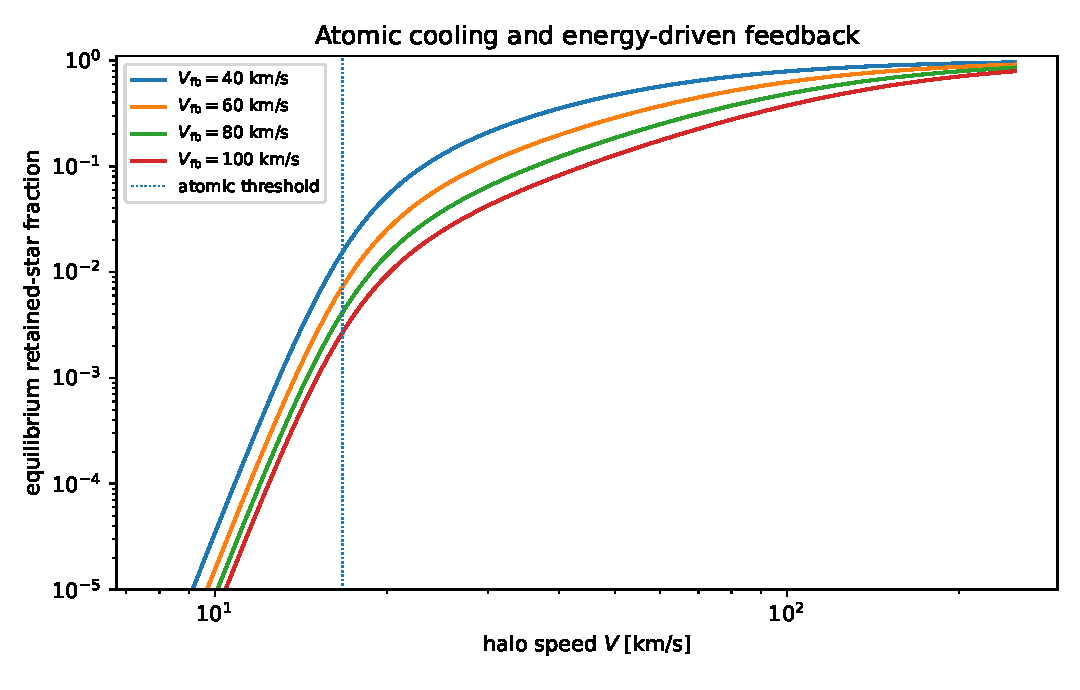
\includegraphics[width=.82\linewidth]{figures/cfr/04_feedback_efficiency.pdf}
\caption{Equilibrium retained star fraction for the declared feedback speeds.  The atomic cooling threshold is fixed by equation \eqref{eq:cfr-atomic-speed}.}
\label{fig:cfr-feedback-efficiency}
\end{figure}

\section{Matched assembly histories}

The paired halo catalogues provide final mass and speed together with the fraction of final particles already contained in the largest progenitor at $a=0.5$.  For each branch, the controlled interpolation is
\begin{equation}
M_h(a)=M_{h,1}a^s,
\qquad
s=
\frac{\log f_{1/2}}{\log(1/2)}.
\label{eq:cfr-growth-history}
\end{equation}
The speed history is normalized to the measured final value,
\begin{equation}
V(a)
=
V_1
\left(
\frac{M_h(a)}{M_{h,1}}
\right)^{1/3}
E(a)^{1/3}.
\label{eq:cfr-speed-history}
\end{equation}

The main matched sample contains $\CFRPairZoom$ pairs.  The time control contains $\CFRPairControl$ pairs.  The response grid contains
\begin{equation}
3\times4\times3\times4\times3=432
\label{eq:cfr-parameter-count}
\end{equation}
common baryonic parameter choices:
\begin{align}
\epsilon_{\rm ff}&\in\{0.005,0.01,0.02\},\\
V_{\rm fb}&\in\{40,60,80,100\}\ {\rm km\,s^{-1}},\\
\beta&\in\{1.5,2,3\},\\
V_{\rm ph}&\in\{15,20,25,30\}\ {\rm km\,s^{-1}},\\
n_{\rm atom}&\in\{2,4,8\}.
\end{align}

For the representative choice
\begin{equation}
(\epsilon_{\rm ff},V_{\rm fb},\beta,V_{\rm ph},n_{\rm atom})
=(0.01,80,2,20,4),
\label{eq:cfr-representative-parameters}
\end{equation}
the aggregate stellar and current star formation ratios approach the final halo mass ratio while retaining a larger early difference.

\begin{figure}[htbp]
\centering
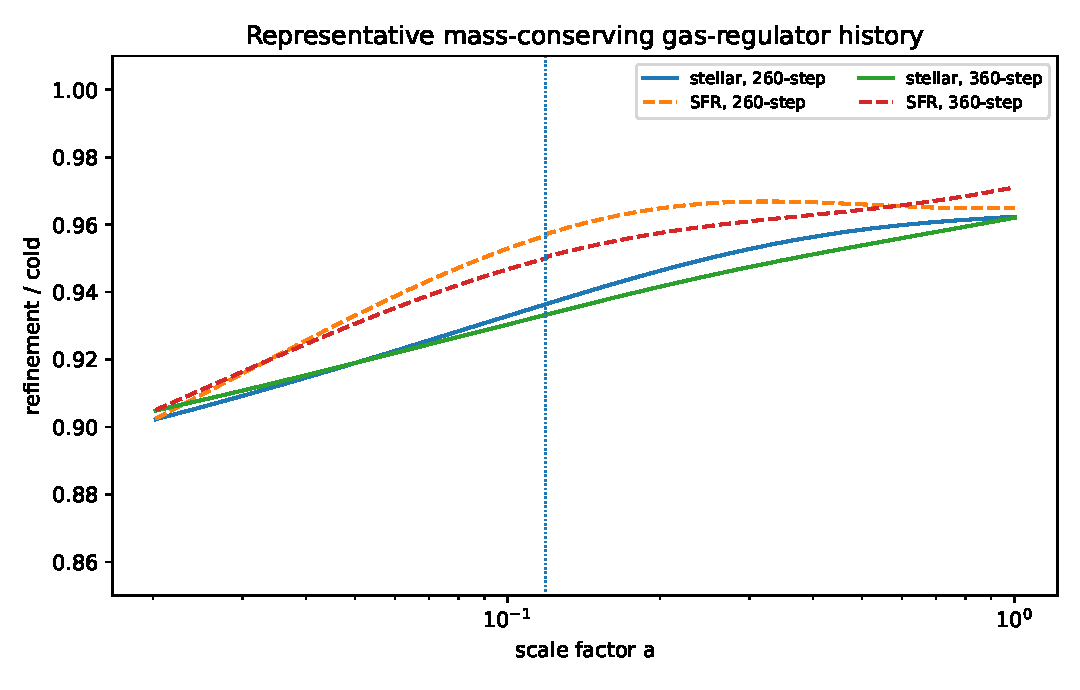
\includegraphics[width=.84\linewidth]{figures/cfr/01_regulator_history.pdf}
\caption{Representative matched sample regulator history.  The vertical marker is the calibrated reionization midpoint.}
\label{fig:cfr-regulator-history}
\end{figure}

\section{Resolved matched baryonic response}

Across the full parameter grid, the matched total stellar ratio is
\begin{equation}
\boxed{
\CFRZoomTotalStarMin
\leq
\frac{M_{\star,R}^{\rm matched}}{M_{\star,C}^{\rm matched}}
\leq
\CFRZoomTotalStarMax
}
\label{eq:cfr-total-star-zoom}
\end{equation}
in the main sample and
\begin{equation}
\boxed{
\CFRControlTotalStarMin
\leq
\frac{M_{\star,R}^{\rm matched}}{M_{\star,C}^{\rm matched}}
\leq
\CFRControlTotalStarMax
}
\label{eq:cfr-total-star-control}
\end{equation}
in the time control.  The medians are $\CFRZoomTotalStarMedian$ and $\CFRControlTotalStarMedian$.

The near cutoff response is much stronger.  For matched cold halos with
\begin{equation}
M_C\leq3\times10^{10}\ M_\odot/h,
\end{equation}
the stellar mass envelopes are
\begin{equation}
\boxed{
\CFRZoomDwarfStarMin
\leq
\operatorname{median}\frac{M_{\star,R}}{M_{\star,C}}
\leq
\CFRZoomDwarfStarMax
}
\label{eq:cfr-dwarf-star-zoom}
\end{equation}
and
\begin{equation}
\boxed{
\CFRControlDwarfStarMin
\leq
\operatorname{median}\frac{M_{\star,R}}{M_{\star,C}}
\leq
\CFRControlDwarfStarMax.
}
\label{eq:cfr-dwarf-star-control}
\end{equation}

The corresponding present star formation rate envelopes are
\begin{equation}
\boxed{
\CFRZoomDwarfSFRMin
\leq
\operatorname{median}\frac{\dot M_{\star,R}}{\dot M_{\star,C}}
\leq
\CFRZoomDwarfSFRMax
}
\label{eq:cfr-dwarf-sfr-zoom}
\end{equation}
and
\begin{equation}
\boxed{
\CFRControlDwarfSFRMin
\leq
\operatorname{median}\frac{\dot M_{\star,R}}{\dot M_{\star,C}}
\leq
\CFRControlDwarfSFRMax.
}
\label{eq:cfr-dwarf-sfr-control}
\end{equation}

Thus the matched total budget is nearly cold like, while the near cutoff stellar mass and current activity are lower by approximately forty percent to sixty percent.

\begin{figure}[htbp]
\centering
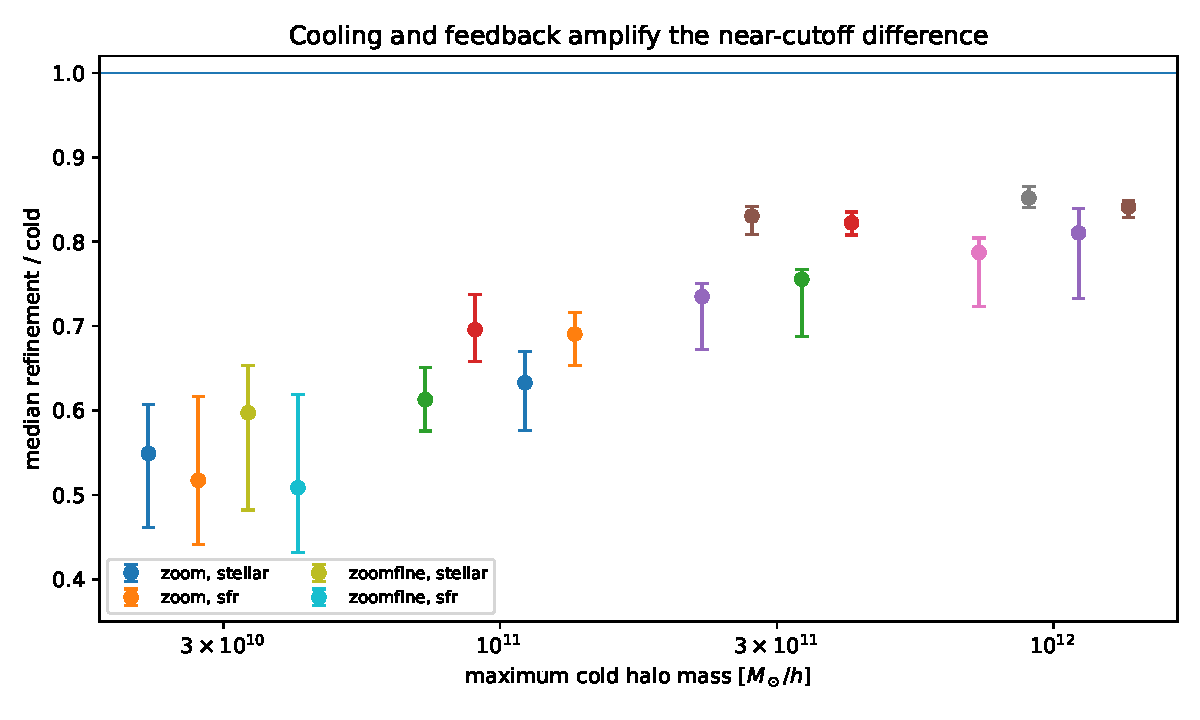
\includegraphics[width=.88\linewidth]{figures/cfr/02_dwarf_response_envelopes.pdf}
\caption{Median stellar mass and present star formation response envelopes as the maximum matched cold halo mass is increased.}
\label{fig:cfr-dwarf-envelopes}
\end{figure}

\section{Ordered source theorem and the assembly boundary}

A strict subset of matched pairs satisfies, throughout the declared history,
\begin{equation}
M_R(a)\leq M_C(a),
\qquad
M_R'(a)\leq M_C'(a),
\qquad
V_R(a)\leq V_C(a).
\label{eq:cfr-source-order}
\end{equation}
There are $\CFROrderedZoom$ such pairs in the main sample and $\CFROrderedControl$ in the time control.

For these source ordered histories, the common regulator produces no integrated stellar ordering violation anywhere in the $432$ point response grid.  The largest ratio is
\begin{equation}
\boxed{
\max
\frac{M_{\star,R}}{M_{\star,C}}
=
\CFRMaxOrderedStar<1.
}
\label{eq:cfr-max-ordered-star}
\end{equation}

Pairs whose assembly histories cross need not obey a pointwise comparison theorem.  Their integrated stellar ratio can depend on when gas entered the halo, not only on the final mass and speed.  This is an important boundary.  A final halo deficit does not by itself determine a unique stellar history.

\section{Feedback weighted ionizing emissivity}

At redshift $z$, let $dn_X/d\log M$ be the cold or refinement halo mass function.  The common equilibrium ionizing source proxy is
\begin{equation}
\dot n_{\gamma,X}(z)
\propto
\int_{M_{\rm atom}(z)}^\infty
M
\epsilon_{\rm src}(M,z)
\frac{dn_X}{d\log M}
\,d\log M,
\label{eq:cfr-ionizing-source}
\end{equation}
where
\begin{equation}
\epsilon_{\rm src}
=
C_{\rm atom}C_{\rm ph}
\frac{1-R}{1-R+\eta_w}.
\label{eq:cfr-source-efficiency}
\end{equation}
The atomic cooling threshold is
\begin{equation}
M_{\rm atom}(z)
=
10^8M_\odot
\left(
\frac{1+z}{10}
\right)^{-3/2}.
\label{eq:cfr-atomic-mass}
\end{equation}
Common photon production and escape factors cancel from the refinement to cold ratio.

At $z=7.4$, including the declared photoheating response,
\begin{equation}
\boxed{
\CFRIonMin
\leq
\frac{\dot n_{\gamma,R}}{\dot n_{\gamma,C}}
\leq
\CFRIonMax,
\qquad
\operatorname{median}=\CFRIonMedian.
}
\label{eq:cfr-ionizing-envelope}
\end{equation}
The required common source efficiency enhancement is
\begin{equation}
\boxed{
\CFRBoostMin
\leq
\frac{\epsilon_{\gamma,R}}{\epsilon_{\gamma,C}}
\leq
\CFRBoostMax,
\qquad
\operatorname{median}=\CFRBoostMedian.
}
\label{eq:cfr-ionizing-boost}
\end{equation}

The earlier unweighted collapsed fraction penalty at the same redshift was $\CFRPriorPenalty$.  Weighting the source toward halos that cool and retain gas reduces the median burden to $\CFRBoostMedian$, but does not remove it.

\begin{figure}[htbp]
\centering
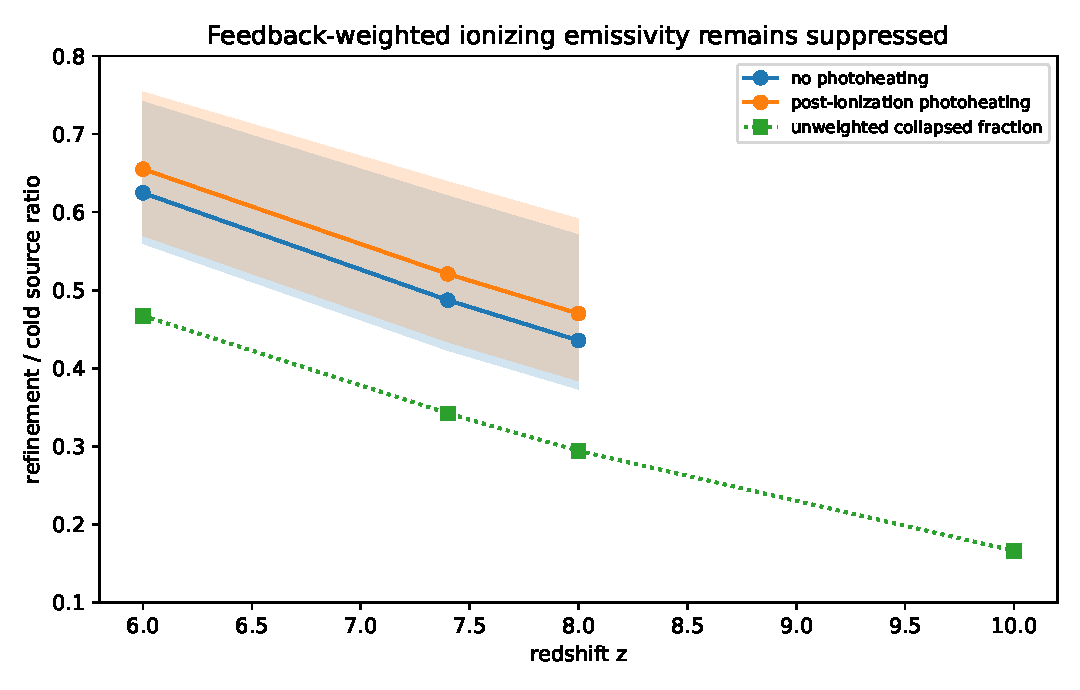
\includegraphics[width=.82\linewidth]{figures/cfr/03_ionizing_emissivity.pdf}
\caption{Feedback weighted ionizing emissivity.  The square markers show the earlier unweighted collapsed fraction ratio.}
\label{fig:cfr-ionizing-emissivity}
\end{figure}

The redshift dependence is
\begin{center}
\begin{tabular}{lccc}
\toprule
redshift & minimum source ratio & median source ratio & maximum source ratio\\
\midrule
$6.0$ & $0.5699$ & $0.6552$ & $0.7539$\\
$7.4$ & $0.4338$ & $0.5208$ & $0.6390$\\
$8.0$ & $0.3841$ & $0.4701$ & $0.5915$\\
\bottomrule
\end{tabular}
\end{center}
The reionization pressure therefore grows rapidly toward earlier epochs.

\section{Scientific interpretation}

The fixed parameter pattern is now more specific:
\begin{equation}
\boxed{
\begin{aligned}
\text{massive matched systems:}&\quad \text{nearly cold like integrated baryon budget},\\
\text{near cutoff systems:}&\quad \text{lower stellar mass and lower present star formation},\\
\text{early ionizing sources:}&\quad \text{suppressed by roughly thirty five percent to sixty percent},\\
\text{reionization:}&\quad \text{requires a source efficiency enhancement of order two}.
\end{aligned}}
\label{eq:cfr-physical-pattern}
\end{equation}

This sharpens the observational hierarchy.  Total stellar mass density is not the strongest discriminator.  Dwarf activity, early galaxies, escape fraction requirements, and the timing of reionization retain more information about the refinement cutoff.

\section{Verification}

The deterministic audit records
\begin{equation}
\boxed{
\CFRPass\ {\rm PASS},
\qquad
\CFRFail\ {\rm FAIL}.
}
\label{eq:cfr-pass-count}
\end{equation}
The checks cover the atomic threshold, the complete parameter grid, sample size, exact mass conservation, positivity, matched total suppression, dwarf stellar and star formation envelopes, source ordered histories, ionizing source suppression, and time control agreement.

\section{Claim boundary}

This chapter establishes an exact mass budget and controlled response calculations within the declared one zone model.  It does not establish:
\begin{itemize}
\item a resolved Euler or magnetohydrodynamic simulation;
\item molecular cooling, metal line cooling, dust, or a multiphase interstellar medium;
\item calibrated stellar populations, supernova yields, or escape fractions;
\item radiation transport or a predicted reionization optical depth;
\item converged subhalos, satellite disruption, or disk shocking;
\item a survey likelihood or empirical correctness;
\item a microscopic derivation of the refinement production scale and coupling.
\end{itemize}

The strongest retained result is not a precision galaxy prediction.  It is a frozen parameter consistency statement:
\begin{equation}
\boxed{
\text{near cold total baryonic budget}
+
\text{strong dwarf and high redshift source suppression}.
}
\label{eq:cfr-retained-signature}
\end{equation}
\chapter{Lagrangian Subhalo Cores, Self-Unbinding, and a Tidal-Survival Audit}
\label{ch:subhalo-core-tidal-audit}
\newcommand{\SCTPass}{20}
\newcommand{\SCTFail}{0}
\newcommand{\SCTCandidates}{27}
\newcommand{\SCTRobust}{23}
\newcommand{\SCTBoundRatio}{0.958333}
\newcommand{\SCTBoundMassZoom}{0.943218}
\newcommand{\SCTBoundMassFine}{0.946203}
\newcommand{\SCTRhalfZoom}{0.975744}
\newcommand{\SCTRhalfFine}{0.963235}
\newcommand{\SCTVmaxZoom}{1.004713}
\newcommand{\SCTVmaxFine}{1.005865}
\newcommand{\SCTHardZoom}{0.772727}
\newcommand{\SCTHardFine}{0.900000}
\newcommand{\SCTSmoothZoomMin}{1.098323}
\newcommand{\SCTSmoothZoomMed}{1.126285}
\newcommand{\SCTSmoothZoomMax}{1.178158}
\newcommand{\SCTSmoothFineMin}{1.101874}
\newcommand{\SCTSmoothFineMed}{1.128740}
\newcommand{\SCTSmoothFineMax}{1.178707}
\newcommand{\SCTLumZoomMin}{1.078604}
\newcommand{\SCTLumZoomMed}{1.120992}
\newcommand{\SCTLumZoomMax}{1.193886}
\newcommand{\SCTLumFineMin}{1.091975}
\newcommand{\SCTLumFineMed}{1.125179}
\newcommand{\SCTLumFineMax}{1.188766}
\newcommand{\SCTStellarZoomMin}{1.018648}
\newcommand{\SCTStellarZoomMed}{1.034769}
\newcommand{\SCTStellarZoomMax}{1.051922}
\newcommand{\SCTStellarFineMin}{1.006992}
\newcommand{\SCTStellarFineMed}{1.025213}
\newcommand{\SCTStellarFineMax}{1.040640}
\newcommand{\SCTCompactZoom}{0.994943}
\newcommand{\SCTCompactFine}{0.981155}


\section{Scope and objective}

The preceding nonlinear calculation resolved paired halo catalogues and showed that near-cutoff refinement halos are less massive, have lower maximum circular-speed proxies, and assemble later than their cold counterparts.  The one-zone baryonic section then showed that these gravitational differences can strongly suppress dwarf stellar activity and high-redshift ionizing production.  A true satellite prediction, however, requires a different object: a self-bound remnant inside a larger host rather than an isolated friends-of-friends component.

This chapter constructs a controlled Lagrangian subhalo-core audit.  It uses particle identities to select matched accreted progenitors at $a=0.5$, follows their particles into five paired host halos at $a=1$, applies a finite spherical self-unbinding map, and compares the resulting cold and refinement remnants.  It then subjects those remnants to a declared tide, disk, and baryonic response envelope.

The principal result is mixed and therefore important:
\begin{equation}
\boxed{
\begin{gathered}
\text{matched refinement remnants contain less bound mass and are slightly smaller},\\
\text{their }V_{\max}\text{ and velocity dispersion remain nearly cold-like},\\
\text{resolved self-bound core counts are almost unchanged},\\
\text{and the sign of a satellite-count correction depends on the unresolved stripping model}.
\end{gathered}}
\label{eq:sct-central-result}
\end{equation}

Thus the present calculation does not support a universal statement that the refinement branch must contain fewer surviving satellites.  It identifies a robust remnant-structure signal and a precise numerical boundary on satellite-count claims.

\section{Matched accreted progenitors}

Let $H_C$ and $H_R$ be a matched cold/refinement host pair at $a=1$.  Let $E_C$ and $E_R$ be a matched pair of halos at $a=0.5$.  The retained accreted-progenitor sample requires:
\begin{align}
N(E_C),N(E_R)&\ge 64,\label{eq:sct-ninit}\\
J(E_C,E_R)&\ge0.2,\label{eq:sct-jaccard}\\
f_{\rm desc,C},f_{\rm desc,R}&\ge0.5,\label{eq:sct-desc}\\
D(E_C)&=H_C,\qquad D(E_R)=H_R.\label{eq:sct-desc-host}
\end{align}
Here $J$ is the particle-ID Jaccard overlap and $D$ is the largest-particle-overlap descendant map.  The principal progenitor of each host is removed so that the sample represents accreted systems rather than the host itself.

The construction gives
\begin{equation}
\boxed{\SCTCandidates\ \text{matched accreted progenitor pairs}}
\label{eq:sct-candidate-count}
\end{equation}
in both the $260$-step run and its $360$-step time control.  After requiring at least twenty self-bound particles in both members of a pair, the structural sample contains
\begin{equation}
\boxed{\SCTRobust\ \text{robust matched remnant pairs}.}
\label{eq:sct-robust-count}
\end{equation}

This Lagrangian construction is stronger than counting neighboring field halos.  Every retained remnant is tied to a declared progenitor and a declared final host by particle identities.

\section{Finite spherical self-unbinding}

For a candidate particle set $S$, choose a robust center $x_S$ and inner-core velocity $v_S$.  For particle $i\in S$, set
\begin{equation}
r_i=\lVert x_i-x_S\rVert,
\qquad
K_i(S)=\frac12\lVert v_i-v_S\rVert^2.
\label{eq:sct-kinetic}
\end{equation}
In the spherical shell approximation, the potential is
\begin{equation}
\Phi_i(S)
=-G\left[
\frac{M_S(\le r_i)}{r_i}
+
\sum_{j\in S:\,r_j>r_i}\frac{m_p}{r_j}
\right].
\label{eq:sct-potential}
\end{equation}
The declared energy criterion is
\begin{equation}
E_i(S)=K_i(S)+\Phi_i(S).
\label{eq:sct-energy}
\end{equation}
Starting from the particles of the early halo that enter the selected final host, define
\begin{equation}
S_{n+1}
=
\{i\in S_n:E_i(S_n)<0\}.
\label{eq:sct-unbinding-map}
\end{equation}

\subsection{Finite-termination theorem}

\textbf{Theorem 61.1.}
For a finite initial set $S_0$, the self-unbinding sequence in \eqref{eq:sct-unbinding-map} stabilizes after at most $|S_0|$ strict-removal steps.

\textbf{Proof.}
By construction,
\begin{equation}
S_{n+1}\subseteq S_n.
\label{eq:sct-nested}
\end{equation}
If the inclusion is strict, at least one particle is removed.  A finite set admits at most $|S_0|$ such removals.  Hence there is an $N\le|S_0|$ with $S_{N+1}=S_N$.  At this fixed point, every retained particle satisfies the declared negative-energy criterion.  \hfill$\square$

The theorem proves finite algorithmic closure.  It does not prove that the fixed point is independent of the center prescription, spherical approximation, force softening, or temporal sampling.

For a stabilized set $S_\infty$, define
\begin{align}
M_b&=m_p|S_\infty|,\label{eq:sct-bound-mass}\\
r_{1/2}&=\operatorname{median}_{i\in S_\infty}r_i,\label{eq:sct-rhalf}\\
\sigma_{1\rm D}^2&=\frac1{3|S_\infty|}\sum_{i\in S_\infty}\lVert v_i-v_S\rVert^2,\label{eq:sct-sigma}\\
V_{\max}^{\rm proxy}&=\sqrt{\frac{GM_b}{r_{1/2}}}.\label{eq:sct-vmax}
\end{align}
The last quantity is a compact structural proxy rather than a converged circular-speed curve.

\section{Resolved self-bound core counts}

The particle-threshold counts are shown in Figure~\ref{fig:sct-thresholds}.  At the central threshold $N_b\ge20$, both time resolutions give
\begin{equation}
\boxed{
N_{C}=24,
\qquad
N_{R}=23,
\qquad
\frac{N_R}{N_C}=\SCTBoundRatio.
}
\label{eq:sct-bound-count}
\end{equation}
At $N_b\ge64$, both branches contain twenty-two remnants in both runs.  Thus the resolved core-count deficit is only one object at the central threshold and disappears at the higher threshold.

\begin{figure}[htbp]
\centering
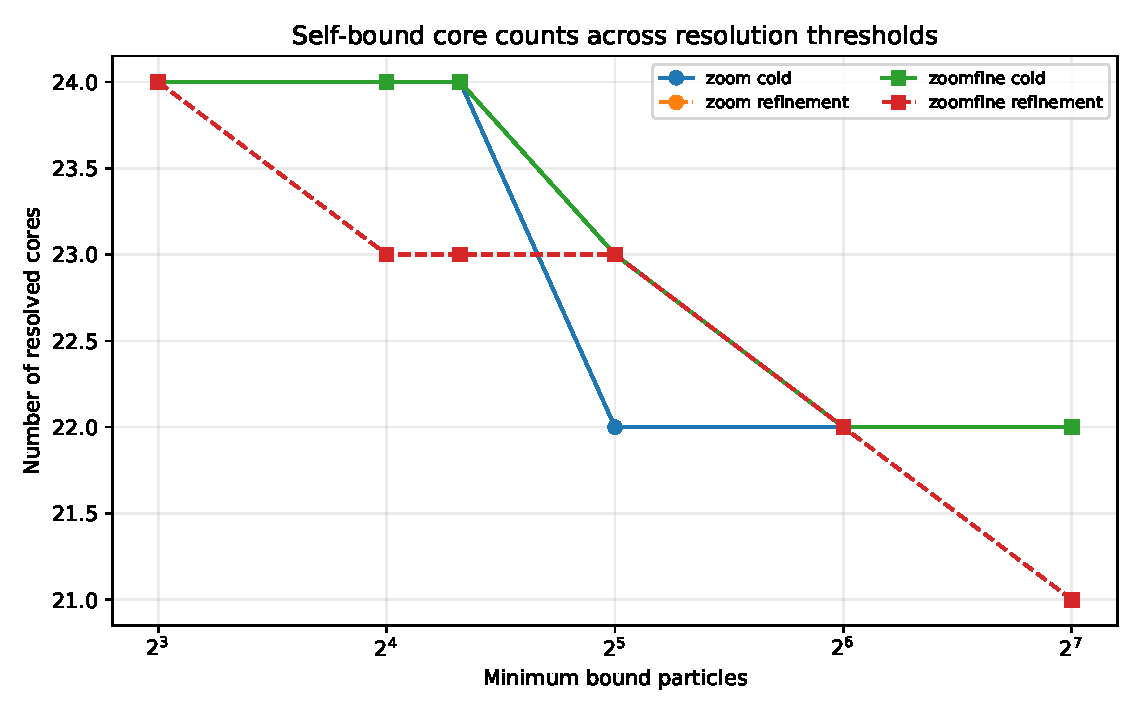
\includegraphics[width=.84\linewidth]{figures/sub/01_bound_core_thresholds.pdf}
\caption{Self-bound remnant counts as the minimum particle threshold is raised.  The cold and refinement curves remain close in both the principal and time-control calculations.}
\label{fig:sct-thresholds}
\end{figure}

This is already a correction to the earlier field-halo intuition.  A deficit in isolated near-cutoff halos does not map one-to-one into a deficit of resolved bound cores inside hosts.

\section{Matched core structure}

For the twenty-three pairs resolved above twenty particles in both branches, the median structural ratios are
\begin{center}
\begin{tabular}{lcc}
\toprule
observable & $260$-step run & $360$-step control\\
\midrule
$M_{b,R}/M_{b,C}$ & \SCTBoundMassZoom & \SCTBoundMassFine\\
$r_{1/2,R}/r_{1/2,C}$ & \SCTRhalfZoom & \SCTRhalfFine\\
$V_{\max,R}/V_{\max,C}$ & \SCTVmaxZoom & \SCTVmaxFine\\
$\sigma_{1\rm D,R}/\sigma_{1\rm D,C}$ & 1.023202 & 1.013546\\
\bottomrule
\end{tabular}
\end{center}

The mass ratios differ between the two time resolutions by less than $0.003$, and the half-mass-radius ratios differ by about $0.013$.  The result is therefore stable at the scale of the present pilot:
\begin{equation}
\boxed{
M_{b,R}\simeq0.945M_{b,C},
\qquad
r_{1/2,R}\simeq0.97r_{1/2,C},
\qquad
V_{\max,R}\simeq V_{\max,C}.
}
\label{eq:sct-structure-summary}
\end{equation}

\begin{figure}[htbp]
\centering
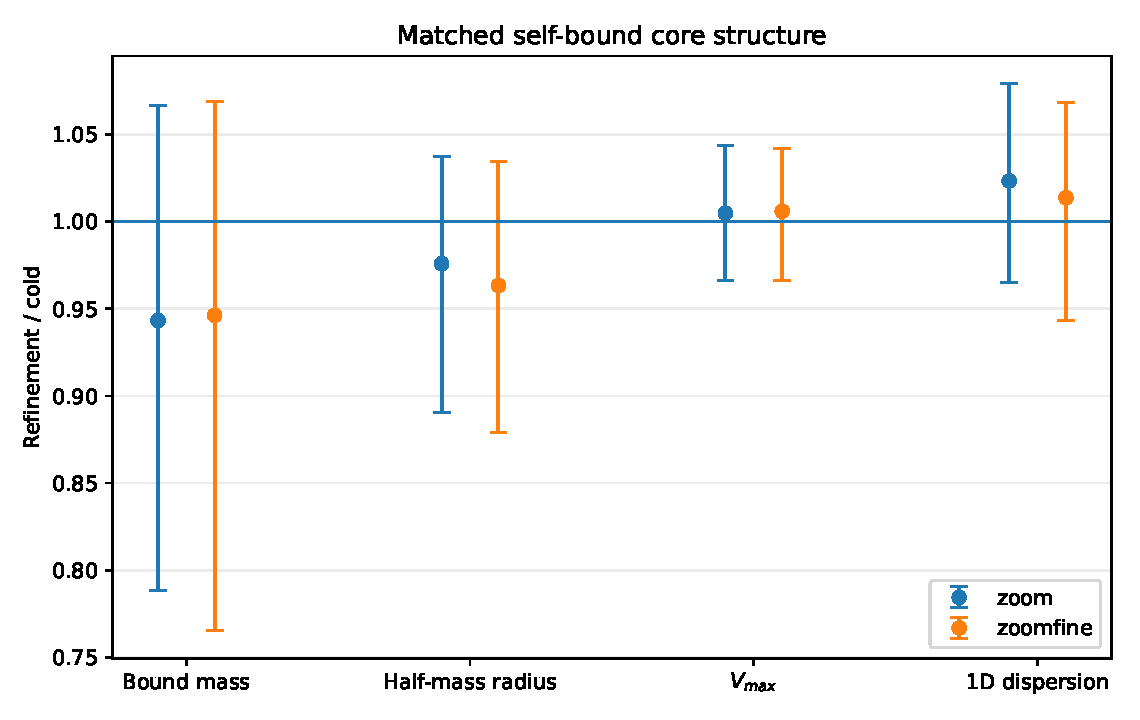
\includegraphics[width=.84\linewidth]{figures/sub/02_core_structure_ratios.pdf}
\caption{Median refinement-to-cold core ratios with $16$th--$84$th percentile intervals.  Bound mass and radius are mildly reduced, while the velocity proxies remain close to unity.}
\label{fig:sct-structure-ratios}
\end{figure}

Approximately seventy percent of the matched remnants have $r_{1/2,R}<r_{1/2,C}$.  The object-by-object mass-size relation is shown in Figure~\ref{fig:sct-mass-size}.

\begin{figure}[htbp]
\centering
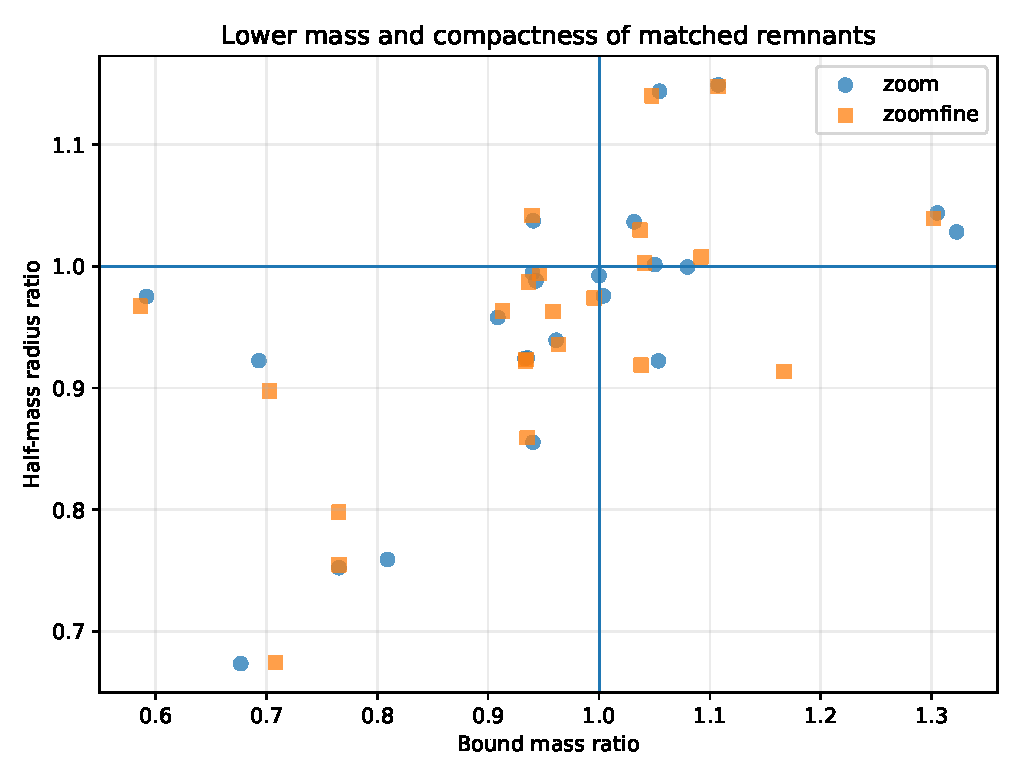
\includegraphics[width=.74\linewidth]{figures/sub/03_mass_size_scatter.pdf}
\caption{Matched bound-mass and half-mass-radius ratios.  The dominant tendency is toward a lower-mass, slightly smaller refinement remnant, although substantial object-to-object scatter remains.}
\label{fig:sct-mass-size}
\end{figure}

\section{Compactness compensation}

For equal host orbit and tidal coefficient, the Jacobi-like tidal radius scales as
\begin{equation}
r_t
=R\left(\frac{M_b}{\kappa M_{\rm host}(<R)}\right)^{1/3}.
\label{eq:sct-rt-simple}
\end{equation}
The ratio of the size-to-tidal-radius variables is therefore
\begin{equation}
\frac{(r_{1/2}/r_t)_R}{(r_{1/2}/r_t)_C}
=
\frac{r_{1/2,R}/r_{1/2,C}}
{(M_{b,R}/M_{b,C})^{1/3}}.
\label{eq:sct-compactness-factor}
\end{equation}
At the median this factor is
\begin{equation}
\boxed{
\mathcal K_{260}=\SCTCompactZoom,
\qquad
\mathcal K_{360}=\SCTCompactFine.
}
\label{eq:sct-compactness-values}
\end{equation}
Both are below unity.  The reduction in physical size compensates for the reduction in mass, so the typical refinement core is not automatically more vulnerable to a common tidal field.

This mechanism explains why a field-halo deficit need not survive as a satellite-core deficit.  The systems that do form in the refinement branch are selected from a colder and more compact surviving population.

\section{Hard current-position tidal proxy}

A separate hard truncation was also applied at the current host-centric radius.  At the twenty-particle threshold it gives
\begin{equation}
\boxed{
\left.\frac{N_R}{N_C}\right|_{\rm hard,260}=\SCTHardZoom,
\qquad
\left.\frac{N_R}{N_C}\right|_{\rm hard,360}=\SCTHardFine.
}
\label{eq:sct-hard-count}
\end{equation}
This proxy suggests fewer refinement remnants, but it changes from $0.773$ to $0.900$ under the time control.  Its sign is stable, but its magnitude is not converged sufficiently for a satellite likelihood.

The hard proxy is sensitive to particle discretization near a sharp tidal boundary.  It should be treated as a negative-control estimate rather than a final count.

\section{Smooth tide, disk, and shock envelope}

To test whether the conclusion depends on sharp truncation, introduce an exponential host disk with mass fraction $f_d$ and scale radius $R_d$.  Its spherical-equivalent enclosed mass is
\begin{equation}
M_d(<R)
=f_dM_{\rm host}\left[1-\left(1+\frac{R}{R_d}\right)e^{-R/R_d}\right].
\label{eq:sct-disk-mass}
\end{equation}
The declared tidal radius is
\begin{equation}
r_t
=R\left[
\frac{M_b}{\kappa\{M_{\rm host}(<R)+M_d(<R)\}}
\right]^{1/3}.
\label{eq:sct-tidal-radius}
\end{equation}
Define the smooth tidal survival weight
\begin{equation}
w_t
=\left[1+\left(\frac{2r_{1/2}}{r_t}\right)^4\right]^{-1}.
\label{eq:sct-tidal-weight}
\end{equation}
A disk-shock proxy is
\begin{equation}
\Xi
=\left[
\frac{2GM_d(<R)r_{1/2}}
{R^2v_{\rm rel}V_{\max}}
\right]^2,
\qquad
w_s=e^{-A\Xi},
\label{eq:sct-shock}
\end{equation}
so that
\begin{equation}
w_{\rm surv}=w_tw_s.
\label{eq:sct-survival-weight}
\end{equation}

The scan contains $144$ tide/disk choices per time resolution:
\begin{equation}
\begin{gathered}
f_d\in\{0,0.01,0.03,0.05\},
\qquad
R_d/r_{90}\in\{0.03,0.06,0.10\},\\
\kappa\in\{2,3,5\},
\qquad
A\in\{0,0.5,1,2\}.
\end{gathered}
\label{eq:sct-gravity-grid}
\end{equation}

The resulting refinement-to-cold survival envelopes are
\begin{equation}
\boxed{
\SCTSmoothZoomMin
\leq
\frac{\sum_iw_{i,R}}{\sum_iw_{i,C}}
\leq
\SCTSmoothZoomMax,
\qquad
\operatorname{median}=\SCTSmoothZoomMed
}
\label{eq:sct-smooth-zoom}
\end{equation}
for the principal run and
\begin{equation}
\boxed{
\SCTSmoothFineMin
\leq
\frac{\sum_iw_{i,R}}{\sum_iw_{i,C}}
\leq
\SCTSmoothFineMax,
\qquad
\operatorname{median}=\SCTSmoothFineMed
}
\label{eq:sct-smooth-fine}
\end{equation}
for the time control.

Every model in this declared smooth envelope lies above unity.  The smaller refinement-core sizes outweigh their lower masses in the survival weighting.  Figure~\ref{fig:sct-disk-scan} shows that this compensation persists as the disk fraction is increased.

\begin{figure}[htbp]
\centering
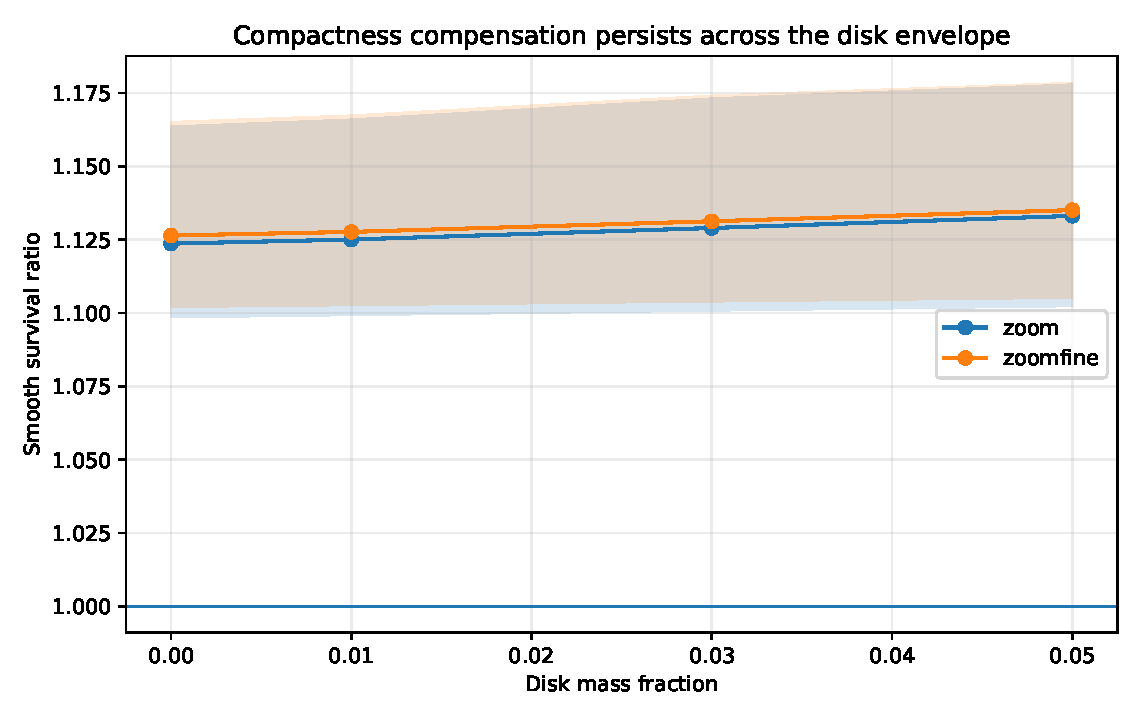
\includegraphics[width=.82\linewidth]{figures/sub/06_disk_fraction_scan.pdf}
\caption{Median and full range of the smooth survival ratio versus disk mass fraction.  Compactness compensation persists throughout the declared tide and shock envelope.}
\label{fig:sct-disk-scan}
\end{figure}

\section{Luminous and stellar survival weights}

A common luminous occupation map is
\begin{equation}
P_{\rm lum}(V)
=\left[
1+\exp\left(-\frac{\log(V/V_{50})}{s}\right)
\right]^{-1}.
\label{eq:sct-luminous-map}
\end{equation}
Scanning
\begin{equation}
V_{50}\in\{15,20,25,30,40\}\ {\rm km\,s^{-1}},
\qquad
s\in\{0.15,0.25,0.40,0.60\},
\label{eq:sct-occ-grid}
\end{equation}
gives the surviving luminous-weight envelopes
\begin{align}
\SCTLumZoomMin
&\leq R_{\rm lum}^{260}\leq\SCTLumZoomMax,
&\operatorname{median}R_{\rm lum}^{260}&=\SCTLumZoomMed,\label{eq:sct-lum-zoom}\\
\SCTLumFineMin
&\leq R_{\rm lum}^{360}\leq\SCTLumFineMax,
&\operatorname{median}R_{\rm lum}^{360}&=\SCTLumFineMed.\label{eq:sct-lum-fine}
\end{align}

A common feedback-weighted stellar proxy uses
\begin{equation}
\epsilon_\star(V)
=C_{\rm atom}(V)C_{\rm ph}(V)
\frac{1-\mathcal R}{1-\mathcal R+(V_{\rm fb}/V)^\beta}.
\label{eq:sct-stellar-efficiency}
\end{equation}
Across thirty-six feedback choices per gravity model, the integrated surviving stellar-weight envelopes are
\begin{align}
\SCTStellarZoomMin
&\leq R_\star^{260}\leq\SCTStellarZoomMax,
&\operatorname{median}R_\star^{260}&=\SCTStellarZoomMed,\label{eq:sct-star-zoom}\\
\SCTStellarFineMin
&\leq R_\star^{360}\leq\SCTStellarFineMax,
&\operatorname{median}R_\star^{360}&=\SCTStellarFineMed.\label{eq:sct-star-fine}
\end{align}

These ratios also exceed unity in the smooth envelope.  They should not be interpreted as a prediction of more observed satellites.  They show that common compactness-dependent survival can offset, and in this model family reverse, the earlier field-halo and dwarf-formation suppression.

\begin{figure}[htbp]
\centering
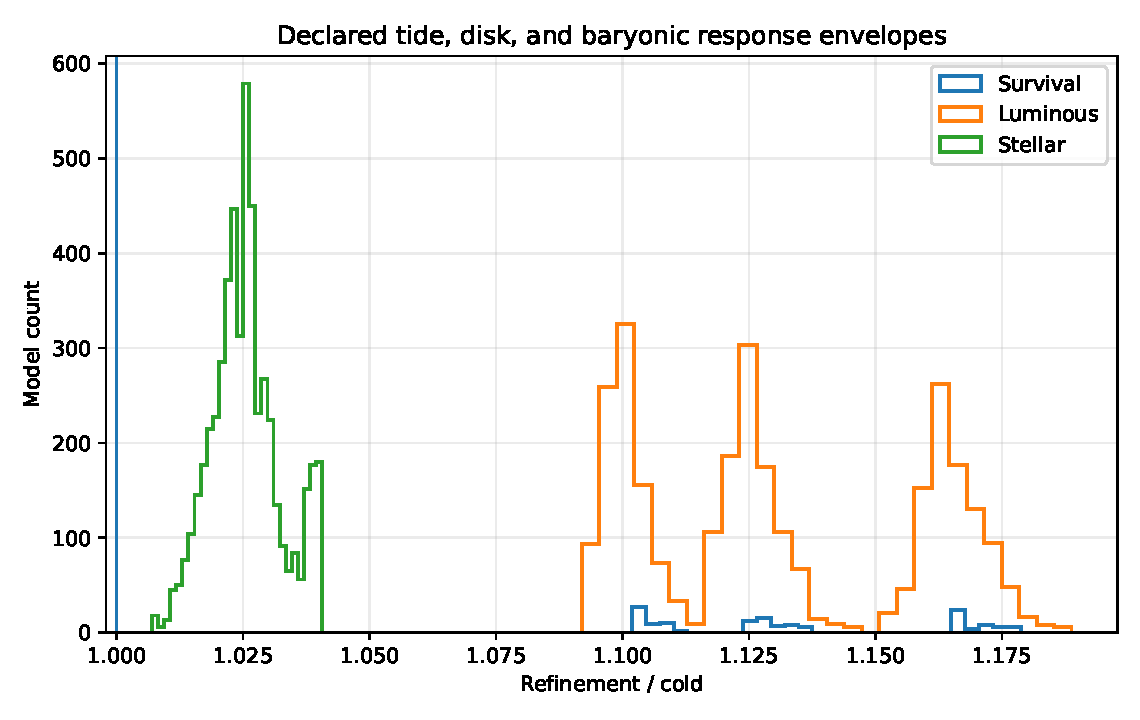
\includegraphics[width=.84\linewidth]{figures/sub/05_survival_envelopes.pdf}
\caption{Distribution of the smooth survival, luminous, and stellar ratios in the $360$-step control.  Every declared model lies above unity, in direct tension with the hard truncation proxy.}
\label{fig:sct-envelope-hist}
\end{figure}

\section{Proxy disagreement and the satellite boundary}

The three retained remnant diagnostics give
\begin{center}
\begin{tabular}{lcc}
\toprule
proxy & $260$-step run & $360$-step control\\
\midrule
self-bound core count, $N_b\ge20$ & 0.958333 & 0.958333\\
hard current tidal count, $N\ge20$ & \SCTHardZoom & \SCTHardFine\\
smooth tide/disk survival envelope & $\SCTSmoothZoomMin$--$\SCTSmoothZoomMax$ & $\SCTSmoothFineMin$--$\SCTSmoothFineMax$\\
\bottomrule
\end{tabular}
\end{center}

The proxies straddle unity.  This is not a nuisance to be hidden.  It is the decisive result of the section:
\begin{equation}
\boxed{
\begin{gathered}
\text{the present spatial and temporal resolution does not determine}\\
\text{the sign of the satellite-count correction}
\end{gathered}
}
\label{eq:sct-no-sign}
\end{equation}

\begin{figure}[htbp]
\centering
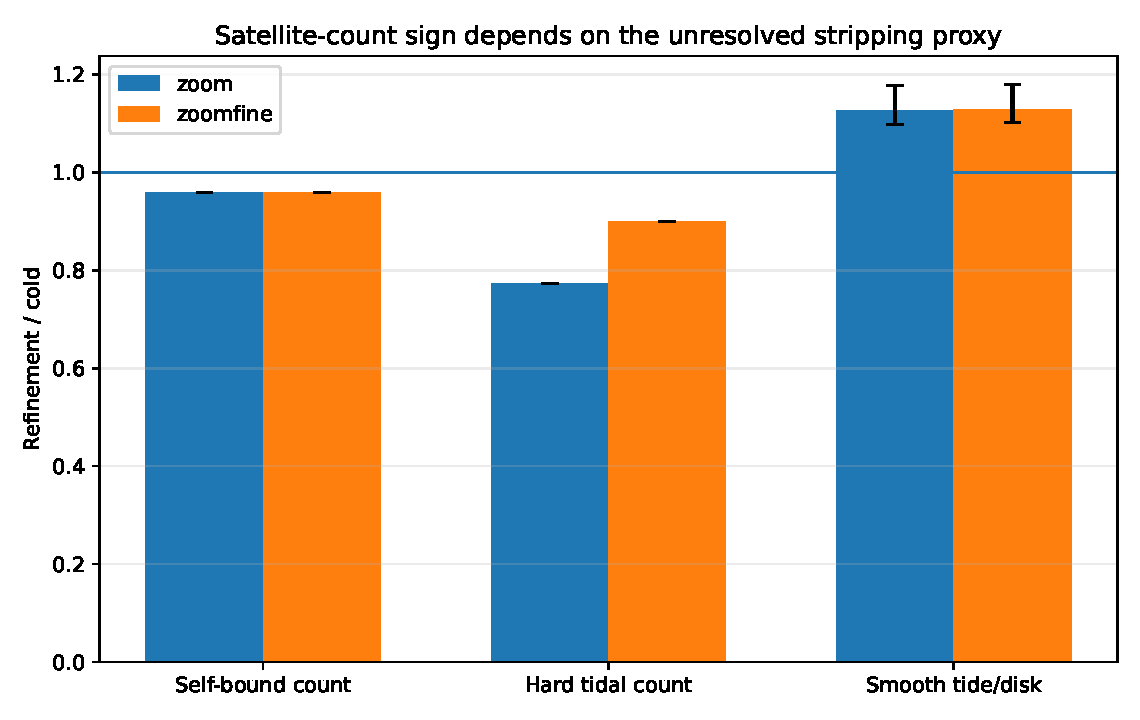
\includegraphics[width=.84\linewidth]{figures/sub/04_proxy_disagreement.pdf}
\caption{The self-bound count, hard tidal cut, and smooth tide/disk envelope do not give one common satellite-count sign.  A resolved host zoom and subhalo finder are required before a satellite likelihood is defensible.}
\label{fig:sct-proxy-disagreement}
\end{figure}

What remains robust is the structural statement:
\begin{equation}
\boxed{
\begin{gathered}
\text{matched refinement remnants are mildly less massive and smaller,}\\
\text{but retain nearly cold-like central velocity scales}
\end{gathered}
}
\label{eq:sct-robust-claim}
\end{equation}

\section{Verification ledger}

The deterministic audit records
\begin{equation}
\boxed{
\SCTPass\ {\rm PASS},
\qquad
\SCTFail\ {\rm FAIL}.
}
\label{eq:sct-pass-count}
\end{equation}
It checks the paired-sample definition, overlap and descendant thresholds, finite self-unbinding termination, particle-threshold counts, structural time control, compactness compensation, finite response scans, and the proxy sign disagreement.

The complete scan contains
\begin{equation}
288\ \text{gravity rows},
\qquad
5760\ \text{luminous rows},
\qquad
10368\ \text{stellar rows}.
\label{eq:sct-scan-counts}
\end{equation}
All archived ratios are finite.

\section{Claim boundary}

This chapter establishes:
\begin{itemize}
\item an exact finite-termination theorem for the declared self-unbinding map;
\item particle-ID-selected accreted progenitor pairs in two time resolutions;
\item controlled self-bound count and matched-structure ratios;
\item a compactness-compensation diagnostic;
\item a declared smooth tide, disk, luminous, and stellar response envelope;
\item a negative result showing that the satellite-count sign is unresolved.
\end{itemize}

It does not establish:
\begin{itemize}
\item a force- and particle-converged subhalo mass function;
\item a six-dimensional phase-space subhalo finder;
\item resolved pericentric stripping or repeated tidal shocks;
\item a live baryonic disk, hydrodynamics, or disk shocking;
\item complete merger trees, orphan satellites, or disruption histories;
\item a survey selection function or satellite likelihood;
\item a microscopic derivation of the refinement production parameters.
\end{itemize}

\chapter{Linked Signatures and Fixed-Parameter Falsifiability}
\PhysicsContext{Linked signatures and physical tests}{The final part turns the calculations into a linked falsification program and distinguishes frozen microscopic parameters from shared astrophysical nuisance parameters.}

\label{ch:linked-falsifiability}
\section{Why linked tests are required}
A flexible model can reproduce one observable by moving nuisance parameters. The refinement dark-sector program is sharper when one microscopic parameter set is propagated through background expansion, kinetic transport, the CMB, nonlinear structure, baryonic response, and subhalo survival without retuning the dark-sector dynamics.
\section{Linked observable pattern}
\begin{equation}\boxed{\begin{gathered}\text{primary CMB and bulk CMB lensing nearly cold-like},\\\text{late nonlinear two-point power strongly regenerated},\\\text{near-cutoff halo abundance and assembly suppressed},\\\text{dwarf stellar activity and high-redshift ionizing sources more strongly suppressed},\\\text{the sign of the final surviving-satellite count unresolved}.\end{gathered}}\end{equation}
This hierarchy is more informative than the generic statement that small-scale power is suppressed.
\clearpage
\section{Erasure thresholds}
For a predicted ratio $R<1$, the branch-dependent enhancement required to erase the difference is
\begin{equation}\Delta_B^{\rm erase}=R^{-1}-1.\end{equation}
Nearly cold CMB-lensing ratios require sub-percent compensation, while dwarf stellar and high-redshift source deficits require order-unity compensation.
\section{Decisive rejection patterns}
The branch would fail or require material revision if a robust joint analysis found any of the following: a matter cutoff inconsistent with the abundance-producing scale; early-galaxy and reionization data incompatible with the frozen transfer under credible source efficiencies; converged subhalo predictions inconsistent with the same halo compactness and assembly response; a locked-mode instability; radiative corrections that destroy the hierarchy without repeated fine tuning; or a joint likelihood that prefers the cold reference after shared nuisance parameters are treated consistently.
\section{What does not yet count as a likelihood}
The response envelopes and normalized spectra in this volume are controlled templates. They do not include a survey covariance, foreground model, selection function, calibration systematics, or posterior sampling. ``Frozen parameter'' means only that dark-sector parameters were not retuned across linked calculations.
\chapter{Open Problems and the Remaining Physical Burden}\label{ch:open-problems}
\section{Production and backreaction}
The specified rapid-crossing spectrum must be replaced or recovered by a controlled coupled field-and-mode calculation. Its energy overdraw is already a concrete obstruction, not a small unquantified uncertainty. Cutoff stability, a conserved renormalized stress tensor, and consistent propagation of the produced spectrum are prerequisites for a microscopic prediction.
\section{Microscopic derivation}
The dominant theoretical gap is the derivation of the physical refinement scale, production epoch $a_\star$, and coupling $\gamma$ from a common microscopic gravitational state.
\section{Quantum and radiative stability}
A complete theory must determine the renormalized effective action, loop stability of the hierarchy, total vacuum-energy accounting, and the fate of locking beyond the Gaussian detail approximation.
\section{Precision transport}
Required work includes precision multilevel recombination and helium kinetics, a production-grade line-of-sight solver, astrophysical reionization, massive neutrinos, full-sky lensing, and comparison with established Boltzmann codes.
\clearpage
\section{Nonlinear structure and baryons}
Required work includes larger volumes, fixed-volume resolution convergence, host zooms, six-dimensional subhalo finding, live disks, hydrodynamics, molecular and metal cooling, radiation transport, star formation, feedback, and survey-calibrated selection.
\section{Statistical establishment}
A decisive data milestone is a joint likelihood with a frozen microscopic parameter map and shared nuisance models across CMB, large-scale structure, lensing, high-redshift galaxies, reionization, and satellites.
\section{External establishment}
Internal audits and second implementations do not establish priority or empirical correctness. External mathematical review, independent numerical reproduction, a complete literature map, and observational model comparison remain separate gates.

\appendix\chapter{Central Formula Guide}\begin{longtable}{@{}P{0.30\textwidth}P{0.62\textwidth}@{}}\toprule Result & Formula\\\midrule Detail multiplicity & $d_h=(p-1)p^{h-1}$\\ Scale-covariant level mass & $m_h^2=m_0^2-\mu^2+\Lambda^2p^{2\sigma h}$\\ Production scale & $\nu_h=A_\star\Lambda p^{\sigma h}$\\ Continuum mass peak & $m_{\rm peak}=5A/(2\pi)$\\ Production equation of state & $w_\star=1/9$\\ Captured rest fraction & $\rho_R/\rho=525\pi/2048$\\ Late cold equation of state & $w_D=a_\star^2/(5a^2)$\\ Locking condition & $M_\phi^2=-\mu^2+(\gamma/v^2)Y_D>0$\\ Release scale & $a_{\rm release}=(\gamma r_{D0}/4)^{1/3}$\\ Gas-regulator budget & $M_g+M_\star+M_{\rm out}=f_bM_h$\\\bottomrule\end{longtable}
\chapter{Specified Benchmark Summary}\begin{longtable}{@{}P{0.48\textwidth}r@{}}\toprule Quantity & Value\\\midrule Production epoch & $a_\star=10^{-6}$\\ Coupling & $\gamma=16$\\ Conditional power half-mode & $k_{1/2}\simeq7.34\ {\rm Mpc}^{-1}$\\ Present $w_D$ & $\simeq2.0\times10^{-13}$\\ Present locking curvature & $M_\phi^2/\mu^2\simeq0.513$\\ Release scale & $a_{\rm release}\simeq1.148$\\ Effective recombination redshift & $z_{\rm rec}\simeq1084.5$\\ Reionization midpoint & $z_{\rm re}\simeq7.41$\\ Half-mode halo mass & $M_{1/2}\simeq1.37\times10^{10}M_\odot$\\ Matched zoom halo mass ratio & $0.834$\\ Matched zoom $V_{\max}$ ratio & $0.944$\\ Ionizing source ratio at $z=7.4$ & median $0.521$\\ Subhalo-core count ratio & $0.958$\\\bottomrule\end{longtable}
\chapter{Reproducibility and Data Map}
The source package contains the manuscript, figures, selected unified-theory data, and namespaced data and verification programs for the collisionless, CMB, thermal-history, lensing, nonlinear-structure, particle-mesh, halo-catalogue, baryonic-response, cooling-feedback, and subhalo-core calculations.

Build with \texttt{Build\_Volume\_II.ps1} or \texttt{Build\_Volume\_II.sh}. A clean rebuild and rendered-page comparison are included in the release audit. These establish package reproducibility, not external independent reproduction.

\section*{Bibliographic scope}\addcontentsline{toc}{section}{Bibliographic scope}
These derivations and computations are not a complete specialist literature-priority audit. Hidden-sector towers, production mechanisms, scalar trapping, Boltzmann methods, CMB solvers, nonlinear structure, and galaxy-formation models each require their own comparative source review. The absence of an exhaustive priority audit limits historical novelty claims and is separate from the conditional mathematical results presented here.
\end{document}
